\documentclass[11pt]{report}

\usepackage[british]{babel}
\usepackage{lipsum} % pack�age to generate filler text Lorem Ip�sum dummy text 
\usepackage[margin=25.4mm,includefoot]{geometry} % geometry package to define margins. Possibility to make left margin larger for binding the document.

\usepackage[hidelinks]{hyperref}  % Allows for clickable reference
\hypersetup{colorlinks = true, linkcolor=blue, citecolor = {blue}, urlcolor=blue,}
\usepackage{enumitem}
%\usepackage[absolute]{textpos}
\usepackage[overlay,absolute]{textpos}

% Graphics preamble
\newcommand\scalemath[2]{\scalebox{#1}{\mbox{\ensuremath{\displaystyle #2}}}}
\usepackage{graphicx} % Alows you to import images
\graphicspath{{figures/}}
\usepackage{caption}
\usepackage{subcaption}
\usepackage{float} % Allows for control of float positions
\usepackage[table,xcdraw]{xcolor}
\usepackage{rotating}
\usepackage{pdflscape}


\usepackage{booktabs}

% Header and Footer Stuff
\usepackage{fancyhdr}   % package for extensive control of page headers and footers
\pagestyle{fancy}
\fancyhead{}
\fancyfoot[C]{\thepage}% Page numbering for center footer
\renewcommand{\headrulewidth}{0pt}    % Removes beautiful line in header
\renewcommand{\footrulewidth}{1pt}
\usepackage[bottom]{footmisc}  % keeps footnotes at bottom of page
\usepackage{multirow}
\setcounter{secnumdepth}{3}
\setcounter{tocdepth}{3}

% Bibliography preamble
\usepackage[round]{natbib}

% Math preamble
\usepackage[short]{optidef} % Why is this package not papering?
\usepackage{amsmath,amssymb,amsthm,mathtools,bm,etoolbox, cases, commath}
\newtheorem{myax}{Axiom}[chapter]
\newtheorem{mydef}{Definition}[chapter]
\newtheorem{myth}{Theorem}[chapter]
\usepackage{algorithm}
\usepackage {algpseudocode}
\usepackage{cases}
\usepackage{bbm}

% Research question preamble
\newtheorem{question}{Question} 
\newcounter{subq} 
\newcommand{\subq}{ 
  \setcounter{subq}{0} 
  \renewcommand\thequestion{\protect\stepcounter{subq}% 
  \arabic{question}\alph{subq}\protect\addtocounter{question}{-1}} 
} 

\newcommand{\normquestion}{ 
  \renewcommand\thequestion{\arabic{question}} 
  \stepcounter{question} 
} 

\usepackage{pdflscape}
\usepackage{everypage}
\newcommand{\Lpagenumber}{\ifdim\textwidth=\linewidth\else\bgroup
  \dimendef\margin=0 %use \margin instead of \dimen0
  \ifodd\value{page}\margin=\oddsidemargin
  \else\margin=\evensidemargin
  \fi
  \raisebox{\dimexpr -\topmargin-\headheight-\headsep-0.5\linewidth}[0pt][0pt]{%
    \rlap{\hspace{\dimexpr \margin+\textheight+\footskip}%
    \llap{\rotatebox{90}{\thepage}}}}%
\egroup\fi}
\AddEverypageHook{\Lpagenumber}%


\begin{document}

\begin{titlepage}
%\begin{center}
\iffalse

\includegraphics[height=2cm]{tue-logo-high}\\

\large
Department of Industrial Engineering and Innovation Sciences  \\
Operations, Planning, Accounting and Control Research Group
\fi
\hfill Eindhoven, July 2018

\vspace*{10cm}

%\setlength{\TPHorizModule}{1mm}
%\setlength{\TPVertModule}{\TPHorizModule}
% Set the Paragraph Indent to zero, so the first line is not Indented
% Back-up the current value so it can be put back at the end of the title page
\newlength{\backupparindent}
\setlength{\backupparindent}{\parindent}
\setlength{\parindent}{0mm}			
\iffalse
\begin{textblock}{165}(45,90)
    \vspace*{1mm}
    \huge
    \textbf{Conditional Correlation Modeling using Multivariate GARCH and Machine Learning \\}
    \Large
    \vspace*{10mm}
    in partial fulfillment of the requirements for the degree of \\
     \vspace*{5mm}
\textbf{Master of Science in \\ Operations Management and Logistics}\\
    \vspace*{10mm}
    \Large
    P.G. Melkert \\
    Student identity number 0893899	
\end{textblock}
\fi
%%%%%%%%%% TUE SPECIFICATION TITLE PAGE %%%%%%%%%%%%
% Textblock width 90 mm, pos x,y (60, 73)
\begin{textblock*}{90mm}(60mm,73mm)
    \vspace*{1mm}
    \Large
    \textbf{Conditional Correlation Modeling \\ using Machine Learning and \\ Multivariate GARCH }
    \vspace*{1mm}    
    
    \normalsize   
    by \\
    Paul G. Melkert \\
\end{textblock*}
\vspace*{15mm}

\begin{center}
Student identity number 0893899	 \\
     \vspace*{15mm}
    in partial fulfilment of the requirements for the degree of \\
     \vspace*{5mm}
\textbf{Master of Science \\ in Operations Management and Logistics}\\
    \vspace*{5mm}



\vfill




\setlength{\parindent}{\backupparindent}
\end{center}

\mbox{}
\vfill
\noindent
Supervisors:\\
Dr. Arun Chockalingam, Eindhoven University of Technology, OPAC \\
Dr. R.J. Almeida, Maastricht University, Quantitative Economics


\clearpage

\noindent
TUE. School of Industrial Engineering. \\
\noindent
Series Master Theses Operations Management and Logistics
\vfill
\noindent
Subject headings: Conditional Correlation; Semiparametric Multivariate GARCH; Nearest Neighbor; Random Forest; Conditional Covariance.  
\vspace{0.5\textheight}

\pagenumbering{gobble}
\end{titlepage} 


\pagenumbering{roman}

\section*{Abstract}    % Asterisk is to remove header numbering (and toc)
\addcontentsline{toc}{section}{\numberline{}Abstract}  % Gets summary in toc

In this paper a new semiparametric multivariate volatility model is proposed, which integrates parametric univariate Generalized Auto Regressive Conditional Heteroskedasticity specifications for the conditional volatilities with nonparametric machine learning estimators k-nearest neighbor and random forest for the conditional correlations. We show that machine learning algorithms can be used to estimate unobserved conditional pairwise correlations between financial returns where imposition of (potentially misspecified) assumptions on the distribution and functional form of the conditional correlation matrix is avoided. Moreover, a parsimonious model specification, with the covariate space constructed using sample correlations from moving windows, ensures that the model remains flexible and easy to estimate in high dimensional systems. First, using simulation, initial insight is provided in the successful application of k-nearest neighbor and random forest estimators for estimation of conditional correlation between financial returns. It is shown that proposed machine learning estimators improve over conventional moving window approximation of conditional correlation by decreasing the sensitivity of results to the choice of window length. Finally, in an empirical application proposed semiparametric multivariate volatility model is applied to the 30 constituents included in the Dow Jones Industrial Average index and model adequacy is verified in terms of common downside market risk measures such as Value-at-Risk and Conditional Value-at-Risk, both in tranquil market conditions such as the mid-1990's and volatile market conditions during the 2000-2001 Dot-com bubble. It is demonstrated that proposed semiparametric multivariate volatility model is able to capture interesting conditional properties in correlations and that it shows competitive performance with a parametric conditionally heteroscedastic class of models, the dynamic conditional correlation model.



\iffalse
This approach not only avoids the rapid increase in parameters as the number of assets becomes large, which typically happens in conventional multivariate conditional volatility models, but also the rigid structure imposed by more parsimonious models, such as the dynamic conditional correlation model. An empirical application to the 30 constituents included in the Dow Jones Industrial Average index demonstrates that the model is able to capture interesting conditional properties in correlations and that it is competitive with standard parametric models in terms of estimating a common risk measure such as Value-at-Risk."
\fi

\iffalse
ref:Hafner2006: "In this paper we develop a new semiparametric model for conditional correlations, which combines parametric univariate Generalized Auto Regressive Conditional Heteroskedasticity specifications for the individual conditional volatilities with nonparametric kernel regression for the conditional correlations. This approach not only avoids the proliferation of parameters as the number of assets becomes large, which typically happens in conventional multivariate conditional volatility models, but also the rigid structure imposed by more parsimonious models, such as the dynamic conditional correlation model. An empirical application to the 30 Dow Jones stocks demonstrates that the model is able to capture interesting asymmetries in correlations and that it is competitive with standard parametric models in terms of constructing minimum variance portfolios and minimum tracking error portfolios."
\fi

\iffalse
In this paper we propose an estimator of the conditional covariance matrix in a quantitive finance setting. Based on the estimation of conditional correlations using machine learning algorithms, this methodology provides an efficient estimator from a semi parametric point of view. \\



\fi




         


\cleardoublepage 

\section*{Acknowledgments}    % Asterisk is to remove header numbering (and toc)
\addcontentsline{toc}{section}{\numberline{}Acknowledgments}  % Gets summary in toc
This work would not have been possible without the support of my university advisors. Therefore, I would like to sincerely thank Dr. Arun Chockalingam and Dr. Rui Almeida for their guidance and flexibility that allowed me to pursue subjects of personal interest throughout these months. I am grateful to them for their interest in this work and for reserving the time to asses it. I would also like to thank Dr. Shaunak Dabadghao for reserving the time to asses this work. 

\cleardoublepage



% Table of Contents stuff
\tableofcontents
\thispagestyle{empty}   % removes page numbering and footer from content page 
\cleardoublepage          % clears the rest of the page

% List of figures, list of tables
\listoffigures
\addcontentsline{toc}{section}{\numberline{}List of Figures}
\cleardoublepage

\listoftables
\addcontentsline{toc}{section}{\numberline{}List of Tables}
\cleardoublepage

\vspace*{\fill} 
\begin{quote} 
\centering 
Essentially, all models are wrong, but some are useful. - \cite{ref:Box1987} 
\end{quote}
\vspace*{\fill}


\clearpage

\newpage\null\thispagestyle{empty}\newpage


% Main body stuff
\pagenumbering{arabic}
\setcounter{page}{1}     % set Introduction as page 1



%NEW CHAPTER 
\chapter{Introduction}\label{sec:intro} 
Correlations are essential inputs for many of the core modeling problems in financial econometrics. Hedges, for example, call for estimates of correlation between the asset returns comprising the hedge. When correlations and volatilities change with the revealing of new information, a proper hedge should reflect the most recent information by adjustment of the hedge ratio. Analogously, derivatives such as rainbow options that comprise two or more underlying assets have prices that are dependent on the correlation between the underlying asset returns. In fact, any pricing formula is premised on estimates of future correlations and volatilities. \\   

\iffalse
"Correlations are critical inputs for many of the common tasks of � financial management. Hedges require estimates of the correlation between the returns of the assets in the hedge. If the correlations and volatilities are changing, then the hedge ratio should be adjusted to account for the most recent information. Similarly, structured products such as rainbow options that are designed with more than one underlying asset have prices that are sensitive to the correlation between the underlying returns. A forecast of future correlations and volatilities is the basis of any pricing formula. 
\fi

\noindent
Correlations are also essential inputs for the tasks of asset allocation and risk management. In this context, however, large systems of correlations are generally required. Portfolio optimization methods used for finding an optimal portfolio given a set of constraints require an estimate of the variance-covariance matrix of future returns. Analogously, calculation of common risk measures such as the standard deviation or Value-at-Risk require estimates of the variance-covariance matrix. These tasks involve estimation of high dimensional variance-covariance matrices, potentially comprising thousands of assets.   \\  

\iffalse
Asset allocation and risk assessment also rely on correlations; however, in this case a large number of correlations is often required. Construction of an optimal portfolio with a set of constraints requires a forecast of the covariance matrix of the returns. Similarly, the calculation of the standard deviation of today's portfolio requires a covariance matrix of all the assets in the portfolio. These functions entail estimation and forecasting of large covariance matrices, potentially with thousands of assets. \\
\fi

\noindent
Modeling of correlations between financial variables has been the topic of academic research for decades. Basic methods such as sample correlations from moving windows and exponential smoothing are commonly used. More involved methods such as univariate generalized autoregressive conditional heteroskedasticity (GARCH) models have been proven adequate to capture certain statistical properties of volatility such as volatility clustering and time-varying or conditional dynamics. In a parametric framework, a variety of multivariate GARCH models has been developed to model the conditional covariances. For some interesting specifications of multivariate GARCH models, see the work of \cite{ref:Bollerslev1988}, \cite{ref:Engle1995}, \cite{ref:Engle1990}, \cite{ref:Ding2001}, \cite{ref:Alexander1997}, \cite{ref:Weide2002}, \cite{ref:Bollerslev1990}, \cite{ref:Engle2001}, \cite{ref:Engle2002}, and \cite{ref:Lanne2007}. A number of studies has provided empirical evidence on the use of multivariate GARCH models for modeling conditional covariance in asset allocation and risk measurement. For examples on high dimensional problems, examine the paper of \cite{ref:Engle2008} and \cite{ref:Laurent2012}. Parametric multivariate GARCH models, however, impose arbitrary assumptions on the distribution and functional form of the conditional covariance matrix. Misspecification of either potentially results in inefficient or inconsistent models.    \\

\iffalse
The quest for reliable estimates of correlations between �financial variables has been the motivation for countless academic articles and practitioner conferences and much Wall Street research. Simple methods such as rolling historical correlations and exponential smoothing are widely used. More complex methods, such as varieties of multivariate generalized autoregressive conditional heteroskedasticity (GARCH) or stochastic volatility, have been extensively investigated in the econometric literature and are used by a few sophisticated practitioners. To see some interesting applications, examine the paper of Bollerslev, Engle, and Wooldridge (1988), Bollerslev (1990), Kroner and Claessens (1991), Engle and Mezrich (1996), Engle, Ng, and Rothschild (1990), Bollerslev, Chou, and Kroner (1992), Bollerslev, Engle, and Nelson (1994), and Ding and Engle (2001). In very few of these articles are more than � five assets considered, despite the apparent need for bigger correlation matrices. In most cases, the number of parameters in large models is too big for easy optimization. \\
\fi

\noindent
An alternative to the parametric estimation of the conditional covariance matrix is provided by non- and semiparametric models. In contrast to parametric estimation, nonparametric models do not impose (potentially misspecified) arbitrary assumptions on the distribution or functional form of the object being estimated. Semiparametric models comprise methods that contain both fully parametric components and fully nonparametric components, and may prove to be appropriate in cases nonparametric models are not;  for example, in case of implications of the curse of dimensionality or lack of knowledge on the distribution of errors \citep{ref:Li2006}. Although semiparametric models may inherit desirable properties of a nonparametric model in that they are robust against misspecification of distributional assumption and functional form, the reliance on parametric assumptions does not exclude semiparametric models from inconsistency. There are numerous papers on nonparametric models for the conditional variance. In contrast, there is a limited number of papers on fully nonparametric multivariate volatility models. For an interesting application, examine the paper of \cite{ref:Long2005}. \\

\noindent
Existing semiparametric multivariate volatility approaches may be based on the premise of a finite-dimensional parameter functional form for the conditional covariance matrix while the error distribution is estimated non- or semiparametrically, or on the premise of a finite-dimensional parameter functional form for either the variances or correlations of the conditional covariance matrix while the other is estimated non- or semiparametrically. For some applications where the error distribution is estimated nonparametrically using kernel functions, examine the work of \cite{ref:Long2005}, \cite{ref:Hafner2007} and \cite{ref:Long2011}\iffalse \footnote{A semiparametric conditional covariance model is proposed that combines parametric and nonparametric estimators of the conditional covariance matrix in a multiplicative way.}\fi. For some interesting Bayesian-based semiparametric multivariate GARCH models, examine the paper of \cite{ref:Jensen2013} \iffalse\footnote{A Bayesian nonparametric modeling approach is proposed for the error distribution in multivariate GARCH models.}\fi and \cite{ref:Virbickait2016}. For some interesting (conditional) copula-based semiparametric multivariate GARCH models\iffalse \footnote{This class of models considers the conditional variance of each marginal time series to be specified parametrically through univariate GARCH-type models where non- or semiparametric estimation of the univariate marginal distributions is followed by a parametric specification of the copula function, which specifies the dependence structure between the marginal series.\fi \iffalse the multivariate distribution of the standardized innovation are specified semiparametrically as a parametric copula evaluated at nonparametric marginals.} \fi, examine the work of  \cite{ref:Chen2006}, \cite{ref:Patton2006}, \cite{ref:Jondeau2006}, \cite{ref:Ausin2010} and \cite{ref:Oh2017}. Finally, for an interesting application belonging to the second category where conditional correlation is estimated nonparametrically, examine the work of \cite{ref:Hafner2006}\iffalse\footnote{A nonparametric estimator is considered for the correlation function where a Nadaraya-Watson kernel regression is applied to each conditional correlation individually.}\fi.  \\

\noindent
The aim of this paper is to develop a new semiparametric model for the conditional covariance matrix that is flexible and remains easy to estimate in high dimensional systems. The model is semiparametric in that it integrates parametric univariate Generalized Auto Regressive Conditional Heteroskedasticity specifications for the conditional volatilities with nonparametric machine learning estimators for the conditional correlations. The choice for machine learning estimators is motivated by the fact that machine learning has been responsible for significant advances in a variety of research areas in the past decade; self-driving cars, speech and facial recognition, effective web search, and medical diagnostic procedures. However, the approach of using machine learning for the estimation of conditional correlation between financial variables has not been extensively investigated in scientific literature. In fact, there is a limited number of papers on this type of machine learning applications. For initial applications, see the papers of \cite{ref:Basturk2016_1} and \cite{ref:Basturk2016}, where a Probabilistic Fuzzy System is used to model the unobserved conditional correlation between financial returns in a bivariate and multivariate setting, respectively. \\

\clearpage

\noindent
In this paper, two nonparametric learning algorithms, k-nearest neighbor and random forest, are considered for point estimating conditional correlations directly and independently of conditional volatilities. These learning methods have a clear advantage over multivariate GARCH models in that any imposition of arbitrary (potentially misspecified) assumptions on the distribution and functional form of the conditional correlation matrix is avoided; the conditional correlations are only assumed to depend on lagged sample correlations obtained using moving window estimation. Moreover, due to a parsimonious model specification, our semiparametric model for the conditional covariance matrix does not suffer from the curse of dimensionality to the same extent as early-stage multivariate GARCH models and many fully nonparametric models. Lack of imposed structure, however, does not guarantee that obtained conditional correlation matrix is positive semidefinite. This is instead verified with obtained correlation coefficients.        \\

\noindent
In this paper, using simulation, performance of conditional correlations estimated by proposed learning methods and conventional moving windows is compared in terms of a statistical loss function, the mean squared error. In an empirical application, proposed semiparametric multivariate volatility model is applied to the 30 constituents included in the Dow Jones Industrial Average index. Model adequacy is verified in terms of an economic loss function, the Value-at-Risk, as the true conditional covariance matrix is unobservable. It is demonstrated that our semiparametric model is able to capture interesting conditional properties in correlations and that it shows competitive performance with a multivariate parametric counterpart, the dynamic conditional correlation model of \cite{ref:Engle2002}.  \\

\noindent
The remainder of the paper is organized as follows. Chapter 2 gives an overview of the methodological underpinnings of multivariate volatility modeling and machine learning. Chapter 3 describes a simulation experiment and out-of-sample results are presented. Section 4 provides an empirical application to the 30 constituents included in the Dow Jones Industrial Average index to test the out-of-sample performance of proposed semiparametric multivariate volatility model. Finally, conclusions and directions for future research are provided in chapter 5. \\

\clearpage


\section{Problem Statement}
The following properties of correlation make the modeling and forecasting of (systems of) correlation(s) inherently complex:

\begin{enumerate}
	\item Correlation is not directly observable.
	\item Correlation between financial variables is time-varying, that is, conditional on the information available at time $t-1$.
	\item Curse of dimensionality: the number of pairwise correlations grows $O(k^2)$ in the number of assets $k$. 
	\item Conditional correlation matrix requires to satisfy positive semidefiniteness.
	\item Any imposition of arbitrary assumptions on the distribution and functional form of the conditional correlation matrix is highly questionable.  
\end{enumerate}

\noindent
This paper will address the last issue by defining the estimation of conditional correlation between financial returns as a supervised learning problem. In defining the task of estimating conditional correlation as a supervised learning problem, unobservability, time-varying property, the curse of dimensionality, and the positive semidefiniteness requirement are considered. Machine learning provides an approach that enables us to extract correlation information without the imposition of arbitrary assumptions on the distribution and functional form of the conditional correlation matrix. Understanding and quantification of conditional correlation between financial returns is an application where any kind of distributional assumption is highly questionable \citep{ref:Christoffersen1998}.  \\


\section{Research Objectives}
The aim of this paper is to develop a new semiparametric model for the conditional covariance matrix that is flexible and remains easy to estimate in high dimensional systems. The model is semiparametric in that it integrates parametric univariate Generalized Auto Regressive Conditional Heteroskedasticity specifications for the conditional volatilities with nonparametric machine learning estimators nearest neighbor and random forest for the conditional correlations. We are interested in the adequacy of proposed semiparametric multivariate volatility model when evaluated against conventional methods. As such, we can formulate the following research objectives:  \\

\begin{enumerate}
	\item Formulate the task of estimating conditional correlation between financial returns as a supervised learning problem.
	\item Given the supervised learning problem formulation, design and implement a nearest neighbor and random forest estimator with support for high dimensional regression output problems.  
	\item Evaluate the machine learning estimators against conventional methods for estimating conditional correlation.  
	\item Evaluate the proposed semiparametric model for the conditional covariance matrix against conventional methods for estimating multivariate volatility.  
\end{enumerate}


\section{Outline and Contributions}
The main contribution of this paper is the development of a computational framework using nearest neighbor and random forest algorithms for the task of estimating conditional correlation between financial returns. We show that the integration of statistical models for capturing conditional volatility, such as univariate GARCH-type models, with proposed learning estimators provides a flexible, semiparametric way of formulating multivariate volatility models that avoid the imposition of (potentially misspecified) assumptions on the distribution and functional form of the conditional correlation matrix. The code used for analysis is provided in a repository at \url{https://github.com/pgm8}. In particular, the machine learning library Scikit-Learn \citep{ref:Pedregosa2011} and (multivariate) GARCH packages rmgarch \citep{ref:Ghalanos2015} and ugarch \citep{ref:Ghalanos2018} have been proven useful in the development of our semiparametric multivariate volatility model.  \\ 

\noindent
Chapter \ref{ch:methodology} presents the methodological framework. The conceptual underpinnings of machine learning (algorithms) and multivariate volatility modeling are discussed. Moreover, an approach is presented to successfully address supervised learning in the context of estimating conditional correlation between financial returns. Given that correlation is not directly observable, construction of the set of covariates and response variables is done by approximation of true correlation using Pearson and Kendall sample correlations from moving windows. The result is a generic and parsimonious supervised learning problem formulation for the task of estimating conditional correlation, which should overcome the difficulty of the curse of dimensionality in high dimensional systems. Notably, the supervised learning problem formulation serves as basis for the first presentation of k-nearest neighbor and random forest estimators of conditional correlation between financial returns. \\

\noindent
Chapter \ref{ch:simulation_study} examines the accuracy of k-nearest neighbor and random forest estimators of correlation in a bivariate setting; two asset return paths with a predefined pairwise correlation structure. The controlled setting of a simulation study allows us to observe the effect of different foundational model properties on the generalization error, which is defined as the mean squared error loss in this chapter. On the premise of mean squared error loss, we are able to observe the effect of incorporation of approximation error due to defining the set of covariates and response variable using moving window estimates of correlation. It is shown that proposed learning estimators improve over conventional moving window approximation of conditional correlation through lower mean squared error and by decreasing the sensitivity of results to the choice of window length in the moving window approximations of conditional correlation. Moreover, learning estimates with approximations of true correlation as covariates and response variable follow the increases and decreases of true correlation smoother, with tighter confidence intervals compared with Pearson and Kendall sample correlation estimates using moving windows. This is a more desirable result as it is not expected that correlation between assets changes that drastically on a daily basis. Additionally, both learning estimators exhibit expected behavior under different parameterizations given the theoretical analysis of mean squared error decomposition into squared bias and variance terms; an increase in the number of neighbors in the nearest neighbor and an increase in the number of decision trees in the random forest reduce the variance in both estimators. Finally, the conditional correlation matrix obtained under a variety of different parameterizations of k-nearest neighbor and random forest estimators satisfy the condition of positive semidefiniteness. In summary, using simulation, initial evidence has been provided on the successful use of proposed learning methods as estimators of conditional correlation between financial returns.  \\

\noindent
We then extend the empirical evaluation of correlation estimates using machine learning to a multivariate setting in chapter \ref{chap:multivariate_analysis}. The focus of analysis is \textit{systems of correlations} in a quantitative financial risk management context rather than \textit{individual correlations}. The proposed semiparametric multivariate volatility model is applied to the 30 constituents included in the Dow Jones Industrial Average index and performance is verified in terms of an economic loss function, the Value-at-Risk (VaR) and Conditional Value-at-Risk, in both tranquil market conditions (mid-1990's) and volatile market conditions (2000-2001 Dot-com bubble). Unconditional coverage and independence tests provide evidence that our semiparametric multivariate volatility model is able to capture interesting conditional properties in correlations and that it is competitive with a fully parametric counterpart, the dynamic conditional correlation (DCC) model of \cite{ref:Engle2002}. The backtest results exhibit general patterns for the 95\%, 97.5\%, and 99\% VaR confidence levels in both market conditions; (1) semiparametric risk model specifications show less conservative behavior compared with the DCC risk model; (2) semiparametric risk model specifications with Kendall approximations of true correlation exhibit a higher number of VaR exceedances than their Pearson counterpart; (3) an increase in the number of neighbors in the nearest neighbor estimator and an increase in the number of decision trees in the random forest estimator result in increased smoothness of estimated VaR levels; (4) the likelihood of a VaR exceedance does not depend greatly on whether a VaR exceedance occurred on the previous day. \\   

\noindent
Finally, chapter \ref{ch:conclusion} contains a general conclusion of this paper as well as interesting directions for future research. The adequate performance of our semiparametric multivariate volatility model is not limited to the specific case of downside market risk assesment and may be extended to other topics in the field of financial econometrics. For future research, it may be interesting to apply proposed semiparametric multivariate volatility model for estimation of the conditional variance-covariance matrix in the context of a multi-stage portfolio optimization problem; it would be interesting to examine proposed semiparametric model's ability to capture multi-stage conditional properties in correlations and volatilities.


\chapter{Methodology} \label{ch:methodology}
In this chapter, we will develop notation and basic approaches that will provide us with the foundational concepts used throughout this paper. Section \ref{sec:mvm} introduces the conceptual underpinnings of multivariate volatility modeling and introduces a class of parametric multivariate GARCH models that is premised on decomposition of the conditional variance-covariance matrix into conditional variances and conditional correlations. Moreover, the semiparametric character of our specification for the conditional covariance matrix will become apparent. Section \ref{sec:ml_supervised} introduces the concepts of machine learning and supervised learning. Theoretical background is given of the learning algorithms that lie at the core of nonparametric learning estimators nearest neighbor and random forest. Furthermore, discussion of an important issue in machine learning, that is, the tradeoff between bias and variance, provides us with the theoretical foundations to study the effect of foundational estimator properties on the generalization error in the simulation study. Finally, section \ref{sec:cor_ml} presents an approach to successfully address supervised learning in the context of estimating conditional correlation between financial returns.

%%%%%%%%%%%%%%%%%%%%%%%%%%%%%%%%%%%%%%%%%%%%%%%%%%%%%%
%%%%%% 				     Multivariate Volatility Methodology 					%%%%%%%
%%%%%%%%%%%%%%%%%%%%%%%%%%%%%%%%%%%%%%%%%%%%%%%%%%%%%%
\section{Multivariate Volatility Modeling} \label{sec:mvm}
Asset allocation and risk management require the identification and quantification of the underlying co-movements in financial returns. This may be captured through specification of the conditional covariance matrix. Following the adequacy of univariate generalized autoregressive conditional heteroskedasticity (GARCH) models in capturing certain statistical properties of conditional volatility, a variety of multivariate GARCH models has been developed to specify the conditional covariance matrix. The different specifications of parametric multivariate GARCH models may be classified into three non-mutually exclusive groups \citep{ref:Bauwens2006}; (1) direct extensions of the univariate GARCH model of \cite{ref:Bollerslev1986}; (2) factor models; (3) models of conditional variances and conditional correlations.    \\

\noindent
Models in the first group specify the conditional covariance matrix directly such as the vector error correction (VEC) model of \cite{ref:Bollerslev1988} and BEKK model of \cite{ref:Engle1995}. These models allow for rich and flexible dynamics of the conditional covariance matrix due to their generality. However, even for low dimensions (3 or 4 assets), the heavily parameterized specifications of VEC and BEKK models become intractable due to the proliferation of parameters, even in restricted parameterizations such as diagonal VEC, diagonal and scalar BEKK. The second group comprises more parsimonious parameterizations of the conditional covariance matrix using factors. Examples are the factor GARCH model of \cite{ref:Engle1990}, the (generalized) orthogonal models of \cite{ref:Alexander1997}, \cite{ref:Weide2002}, and \cite{ref:Lanne2007}. For a more a comprehensive survey of these models, examine the work of \cite{ref:Bauwens2006}. Models in the third group are parsimonious in parameterization and premised on decomposition of the conditional covariance matrix into conditional variances and conditional correlations, which are then modeled separately. These models were first introduced through the constant conditional correlation (CCC) model of \cite{ref:Bollerslev1990}, which assumed (unrealistically) correlations to be constant over time. Generalization of the CCC model was proposed by \cite{ref:Engle2002} and \cite{ref:Tse2002}. These dynamic conditional correlation models allow for both the conditional variance matrix and conditional correlation matrix to be time-varying. Moreover, the formulation of our semiparametric multivariate volatility model is premised on decomposition of the conditional covariance matrix into conditional variances and conditional correlations.   \\

\noindent
As such, in this paper, a mean-corrcted $k$-dimensional log return series, $r_t = (r_{1,t}, \dots, r_{k,t})'$, is considered such that

\begin{align} 
	r_t = H^{1/2}_t z_t \label{eq:returns_model}
\end{align}

\noindent
where $t \in \{1, \dots,T\}$ indicates the time unit, $z_t$ is a $k \times 1$ vector of independent and identically distributed random variables with mean zero and unit variance, $H_t$ is a $k\times k$ positive semidefinite matrix, and $H_t^{1/2}$  denotes the Cholesky decomposition of $H_t$. \\

\noindent
The conditional variance-covariances of returns $r_t$ are represented by the $k \times k$ matrix $\mathrm {Var}(r_t) = H^{1/2}_t H^{\prime 1/2}_t = H_t$, which is not observable by construction \citep{ref:Basturk2016}. A plethora of models has been proposed to model the conditional covariance matrix $H_t$ and we consider a reparameterization of $H_t$ that is a common approach for the identification of variances and correlation coefficients \citep{ref:Bauwens2006}, that is, 

\begin{align} \label{eq:covariance_decomposition} 
	H_{t}=D_{t}R_{t}D_{t} = 
		\begin{pmatrix} h_{1,1,t}^{1/2} &&0 \\ &\ddots \\ 0 &&h_{k,k,t}^{1/2} \end{pmatrix} 
		\begin{pmatrix} 1 &\rho_{1,2,t} &\cdots &\rho_{1,k, t} \\ \rho_{2,1,t} &1 & &\rho_{2,k, t} \\ \vdots &&\ddots &\vdots \\ \rho_{k, 1,t} &\rho_{k, 2,t} &\cdots &1 \end{pmatrix} 
		\begin{pmatrix} h_{1,1,t}^{1/2} &&0 \\ &\ddots \\ 0 &&h_{k,k,t}^{1/2} \end{pmatrix} 
\end{align}

\noindent
where $D_t$ is a diagonal matrix with conditional volatility of each marginal series on its diagonal and matrix $R_t$ includes all pairwise correlations $\rho_{i,j,t}$, with $\rho_{i,j,t} = \rho_{j,i,t}$ (by definition). \\

\iffalse
\begin{align} \label{eq:covariance_decomposition} 
		\begin{pmatrix} \sigma_{1}^2 &\sigma_{1}\sigma_{2}\rho_{1,2} &\cdots &\sigma_{1}\sigma_{k}\rho_{1,k} \\ \sigma_{2}\sigma_{1}\rho_{2,1} &\sigma_{2}^2 & &\sigma_2\sigma_k\rho_{2,k} \\ \vdots &&\ddots &\vdots \\ \sigma_k\sigma_1\rho_{k, 1} &\sigma_k\sigma_2\rho_{k, 2} &\cdots &\sigma_{k}^2 \end{pmatrix} 
\end{align}
\fi

\noindent
The semiparametric character of our specification for $H_t$ now becomes apparent: the diagonal elements of the matrix $D_t$ are modeled parametrically using, for example, univariate GARCH-type models, whereas the conditional correlation matrix $R_t$ is estimated in a nonparametric manner using nonparametric machine learning algorithms. Estimation of $D_t$  is independent of the estimation of pairwise correlations, $\rho_{i,j,t}$, in $R_t$. This is explained by the fact that $D_t$ defines the unconditional variance of each marginal series at time unit $t$ and is, by definition, independent of correlations $R_t$ \citep{ref:Basturk2016}. In order to ensure positive semidefiniteness of the conditional covariance matrix $H_t$ at each time unit $t$, two necessary conditions need to be satisfied when specifying $R_t$, that is,  

\begin{enumerate}
	\item $R_t$ has to be positive semidefinite with det($R_t) > $ 0. ($D_t$ is positive semidefinite as all its diagonal elements are positive).
	\item The absolute value of all elements in the conditional correlation matrix $R_t$ need to be equal to or less than one by definition. 
\end{enumerate}

\noindent
These necessary conditions for satisfying a positive semidefinite matrix $R_t$ are generally obtained by the imposition of arbitrary assumptions on the distribution and functional form of the conditional correlation matrix. In view of the fact that many nonparametric estimators of the covariance matrix are developed without explicit satisfaction of the positive semidefiniteness condition during estimation, satisfaction of the conditions is in this paper verified with the obtained conditional correlation matrix. \\     

\noindent
We examine the parametric dynamic conditional correlation model in further detail in the next section as our semiparametric multivariate volatility model specification will be evaluated against this model in chapter \ref{chap:multivariate_analysis}.

\subsection{Dynamic Conditional Correlation Model} \label{sec:dcc}
The dynamic conditional Correlation (DCC) model of \cite{ref:Engle2002} is a class of models that generalizes univariate GARCH models to the multivariate case. The DCC models capture the advantages of GARCH models but are parsimonious in parameterization and computation compared with the multivariate GARCH models such as VEC and BEKK. Premised on decomposition of the conditional covariance matrix into conditional variances and conditional correlations lets the DCC model take advantage of the fact that the conditional correlation matrix is generally easier to model than direct modeling of the conditional covariance matrix. In the DCC models, time series of daily mean-corrected log returns on k assets $r_t=a_t$ is given by

\begin{align}
	r_t &= H_t^{1/2}z_t \\
	H_t &= D_t R_t D_t \\
	D_t &= diag(\sigma_{1,t}, \dots, \sigma_{k,t})
\end{align}

\noindent
where $H_t$ is the conditional covariance matrix and $R_t$ is the conditional correlation matrix. $D_t$ is a diagonal matrix with $\sigma_{1,t}, \dots, \sigma_{k,t}$ on the main diagonal, which can be estimated though univariate GARCH models. \\

\noindent
The idea behind DCC models is that multivariate volatility modeling can be divided into two estimation steps. Under assumption of conditional normality in the daily mean-corrected log returns $r_t$, the estimator gives rise to a log likelihood function. Without this assumption, an expected Quasi-Maximum Likelihood function is calculated \citep{ref:Engle2002}. As such, the first step is to estimate the conditional volatility series, $\sigma_{i,t}$, which is done under the assumption that marginal volatility series follow a univariate GARCH(1,1) process with Gaussian distributed errors, that is,

\begin{align}
	\sigma_{i,t}^2 &= \omega_i + \beta_i\sigma_{i,t-1}^2 + \alpha_i a_{i,t-1}^2 
\end{align}

\noindent
Then, in the second step, one can use the estimated conditional volatilities $\sigma_{i, t}$ to model the dynamics of the conditional correlation matrix $R_t$, that is,

\begin{align}
	R_t &= D_t^{-1} H_t D_t^{-1}
\end{align}     
 
\noindent
$R_t$, as noted by \cite{ref:Engle2002}, is the conditional volatility matrix of the marginally standardized residuals $\epsilon_t = (\epsilon_{1,t}, \epsilon_{2,t}, \dots, \epsilon_{k,t})$, where $\epsilon_{i,t} = a_{i,t} / \sigma_{i,t}$. In this paper, the multivariate standard normal is considered for the conditional distribution $\epsilon_t$. \\

\noindent
In the DCC model of \cite{ref:Engle2002}, the conditional volatility matrix of the marginally standardized residuals, $\epsilon_t$, is modeled using a GARCH(1,1) specification and reparameterization of $R_t$ ensures necessary conditions for $R_t$ are satisfied, that is,

\begin{align}  
	Q_t &= (1-\theta_1-\theta_2) \bar{Q} + \theta_1 Q_{t-1} \theta_2 \epsilon_{t-1} \epsilon'_{t-1} \label{eq:DCC_Q} \\
	R_t &= diag(Q_t)^{-1} Q_t \ diag(Q_t)^{-1} \label{eq:DCC_R}
\end{align}

\noindent
In \eqref{eq:DCC_Q}, $Q_t$ is a positive semidefinite matrix defining the structure of the correlation dynamics and $\bar{Q} = Cov(\epsilon_t \epsilon'_t) = \mathbb{E}[\epsilon_t \epsilon'_t]$ is the unconditional covariance matrix of the standardized residuals $\epsilon_t$\footnote{$\bar{Q}$ can be thought of as representing the long-run correlation structure and can be estimated by: $\bar{Q} = \frac{1}{T} \sum_{t=1}^T \epsilon_t \epsilon'_t$.}. In \eqref{eq:DCC_R}, $diag(Q)_t$ is a diagonal matrix with the square root of the diagonal elements of $Q_t$ at its diagonal. It is simply a normalization matrix to ensure the requirement that all elements in the conditional correlation matrix $R_t$ are bounded by -1 and 1. Parameters $\theta_1$, $\theta_2$ are non-negative real numbers satisfying $ 0 < \theta_1 + \theta_2 < 1$, which ensures $Q_t$ to satisfy the condition of a positive semidefiniteness and consequently positive semidefiniteness for $H_t$ under the condition that $D_t$ is also positive semidefinite.\\ 

\noindent
Eq. \eqref{eq:DCC_Q} shows that the DCC model of \cite{ref:Engle2002} is very parsimonious as the dynamics of all conditional correlations are driven with only two parameters, $\theta_1$ and $\theta_2$, regardless of the number of assets $k$. This is a necessary condition to ensure positive semidefiniteness of $R_t$ for all time $t$. Consequently, the DCC model is relatively efficient to estimate and remains tractable when $k$ grows large. However, the assumption that the evolution of all correlations follows the same dynamic structure, regardless of the assets involved, can be considered a weakness of the DCC model, especially in high dimensional systems comprising many asset return series. \\

\iffalse
\noindent
\textbf{The approximation used for one-step-ahead forecasts can be found in \cite{ref:Engle2001}}. \\
\fi



\subsection{Pearson Product-Moment Correlation Coefficient}
One method to estimate pairwise correlation coefficients $\rho_{i,j,t}$ in the conditional correlation matrix $R_t$ is to use sample correlations from moving windows. An advantage of this method is that it avoids strong distributional assumptions. Following \cite{ref:Basturk2016}, the sample correlation at a selected time window $\Delta t$ is used as a proxy for approximation of conditional correlation using Pearson's linear correlation coefficient, that is,

\begin{align}
	\hat{\mu}_{i,t} &= \frac{1}{\Delta t}\sum\nolimits_{t'=t-\Delta t+1}^t r_{i,t'}, \; \; \forall i \in \{1, \dots, k\} \label{eq:mw_mu} \\
	\hat{\sigma}_{i,t} &= \sqrt{\frac{1}{\Delta t}\sum\nolimits_{t'=t-\Delta t+1}^t (r_{i,t'}-\hat{\mu}_{i,t})^2}, \; \; \forall i \in \{1, \dots, k\}   \label{eq:mw_sigma} \\ 
	\hat{\sigma}_{i,j,t} &= \frac{1}{\Delta t} \sum\nolimits_{t'=t-\Delta t+1}^t (r_{i,t'}-\hat{\mu}_{i,t})(r_{j,t'}-\hat{\mu}_{j,t})  \; \; \forall i,j \in \{1, \dots, k\}   \label{eq:mw_cov} \\ 
	\hat{\rho}_{i,j,t} &= \frac{\hat{\sigma}_{i,j,t}}{\hat{\sigma}_{i,t} \hat{\sigma}_{j,t}} \label{eq:mw_rho} 
\end{align}   

\noindent
where $\hat{\mu}_{i,t}$ defines the mean estimate for random variable $i$ at time $t$, $\hat{\sigma}_{i,t}$ defines an estimate of the standard deviation for random variable $i$ at time $t$, and $\hat{\sigma}_{i,j,t}$ defines the covariance between random variables $i$ and $j$ at time $t$. Consequently, the Pearson product-moment correlation coefficient between random variables $i$ and $j$ at time $t$ is defined by $\hat{\rho}_{i,j,t}$. \\

\noindent
Note that the correlation coefficient is dimensionless and, by definition, takes values between $-1$ and $1$. If the correlation between two random variables is close to $|1|$, then that is an indication of a strong linear relationship between corresponding random variables. The nonparametric learning estimators proposed in this paper make use of the moving window correlation estimates in \eqref{eq:mw_mu}-\eqref{eq:mw_rho} to define the set of covariates and response variable.

\iffalse
Additionally, exponential weighting of correlation coefficients $\rho_{i,j,t}$ is included in the analysis. Introduction of exponential weighting, where present observations are given more weight than past measurements, potentially better characterizes the dynamics of evolving dependency structures between asset return paths. From an informational point of view it makes sense to assume recent events more valuable than remote ones. For the computation of weighted Pearson correlation coefficients a weight structure, $w_t \ge 0$, is introduced under the constraint $\sum_{t'=t-\Delta t+1}^t w_t = 1$, operating on sample means, variances and covariances according to \cite{ref:Pozzi2012}:

\begin{align}
	\hat{\mu}_{i,t}^w &= \sum_{t'=t-\Delta t+1}^t w_{t'} y_{i,t'}, \; \; \forall i \in \{1, \dots, k\} \label{eq:mw_mu_w} \\
	\hat{\sigma}_{i,t}^w &= \sqrt{\sum\nolimits_{t'=t-\Delta t+1}^t w_{t'} (y_{i,t'}-\hat{\mu}_{i,t}^w)^2}, \; \; \forall i \in \{1, \dots, k\}   \label{eq:mw_sigma_w} \\ 
	\hat{\sigma}_{i,j,t}^w &= \sum\nolimits_{t'=t-\Delta t+1}^t w_{t'} (y_{i,t'}-\hat{\mu}_{i,t}^w)(y_{j,t'}-\hat{\mu}_{j,t}^w)  \; \; \forall i,j \in \{1, \dots, k\}   \label{eq:mw_cov_w} \\   
	\hat{\rho}_{i,j,t}^w &= \frac{\hat{\sigma}_{i,j,t}^w}{\hat{\sigma}_{i,t}^w\hat{\sigma}_{j,t}^w} \label{eq:mw_rho_w} 
\end{align}  

\noindent
\cite{ref:Pozzi2012} use the exponential function as functional form for the weights, i.e. exponential smoothing. This is the kind of weighting also used in this paper such that the weights in \eqref{eq:mw_mu_w}-\eqref{eq:mw_rho_w} are defined as:

\begin{align} \label{eq:pearson_weights}
	w_{t'} = w_0 \; e^{\alpha(t'- \Delta t)}, \; \; \forall t' \in \{t-\Delta t+1, t-\Delta t, \cdots, t\} 
\end{align}   

\noindent
where $\alpha = \frac{1}{\theta}$ denotes the exponential decay factor, with $\alpha \in \mathbb{R}$ and $\alpha \ge 0$, and $w_0(\alpha) = \frac{1-e^{-\alpha}}{1-e^{-\alpha\Delta t}}$. Intuitively, when the parameter $\theta$ gets arbitrarily large, i.e. as $\theta \rightarrow \infty$, the weights are uniform and no distinction is made between the informational value of recent events and more remote ones. Conversely, lower values for $\theta$ indicate remote events to become increasingly irrelevant and more recent ones become ever more relevant from an informational point of view \citep{ref:Pozzi2012}. In this paper $\theta = \frac{\Delta t}{3}$ following the statement of \cite{ref:Pozzi2012} that "it is a reasonable choice for their data-set."  \\
\fi

\subsection{Capturing Nonlinear Relations: Kendall's $\tau$} 
The Pearson product-moment correlation coefficient is the most frequent used measure for testing dependency between random variables. It is, however, only a measure of linear dependence and using a linear correlation coefficient as a measure of dependence may lead to erroneous inferences outside the domain of elliptical distributions \citep{ref:Aas2004}. Given the fact that asset returns are generally not well represented by an elliptical distribution and exhibit non-linear dependence, alternative methods for capturing co-dependency are considered in this paper. One such alternative method is Kendall rank correlation coefficient, commonly referred to as Kendall's $\tau$ correlation coefficient \citep{ref:Kendall1948}, which measures the degree of similarity between two random variables through counting the concordant and discordant pairs. Kendall's $\tau$ accounting for tied pairs is formulated as

\begin{align} \label{eq:mw_kendall}
	\hat{\tau}_{i,j} = \frac{\sum_{u=1}^{\Delta t -1} \sum_{v=u+1}^{\Delta t} d_{uv}^i d_{uv}^j}{\sqrt{[\frac{1}{2}\Delta t (\Delta t -1)-n^i][\frac{1}{2}\Delta t(\Delta t - 1)-n^j]}}
\end{align}

\noindent
where $d^k = sgn (r_u^k - r_v^k)$ for $k = i, j$ and $n^k$ is the total number of tied pairs for variable $k$. \\

\noindent
Kendall's $\tau$ rank correlation has some desirable theoretical properties over Pearson product-moment correlation such as: Kendall's $\tau$ rank correlation is able to capture nonlinear relationships and it is a distribution free measure, that is, it is independent of the statistical distribution of the variables. It is robust to outliers and remains well defined for random variables with infinite variance. Moreover, Kendall's correlation matrix generally maintains positive semidefiniteness. A limit to the use of Kendall's $\tau$ rank correlation on large samples is its computational complexity of $O(\Delta t \ log \ \Delta t)$ \citep{ref:Pozzi2012}. This will however not be an issue in this paper as the sample size of the empirical application in chapter \ref{chap:multivariate_analysis} does not qualify as problematic large.  \\

\noindent
Similar to Pearson moving window estimates of correlation, Kendall's $\tau$ correlation coefficient takes values in the interval [$-1$, $1$]. Values close to $1$ indicate strong similarity whereas values close to $-1$ indicate strong dissimilarity. In addition to Pearson moving window correlation estimates, as defined in \eqref{eq:mw_mu}-\eqref{eq:mw_rho}, the nonparametric learning estimators proposed in this paper make use of the moving window correlation estimates in \eqref{eq:mw_kendall} to define the set of covariates and response variable. \\

\section{Machine Learning} \label{sec:ml_supervised}
Machine learning is the science of getting computers to gain the ability to learn from data without any user imposed conditions, that is, without being explicitly programmed. In a typical machine learning setting, one has an outcome measurement, generally quantitative (e.g. asset price) or categorical (e.g. septic/ not septic) in nature, that one wishes to predict based on a set of predictor variables or covariates (e.g. blood pressure, body temperature and heart rate). One possesses a training set of data, in which the outcome and covariate measurements for a set of objects (e.g. people or days in case of time series analysis) is observed. Then, this data serves to build a prediction model, or learner, which will have the purpose of enabling one to predict the outcome for new unseen objects or input instances. An adequate learner is one that is capable of accurately predicting such an outcome. The goal of the learning process is to progressively improve the learner's performance on a specific task.  \\

\noindent
The example above describes a particular type of machine learning problem, namely a \textit{supervised learning problem}. The qualification \textit{supervised} comes from the fact that the outcome variable is present to guide the learning process. More formally: a supervised learning problem is concerned with the prediction of one or more outputs or response variables $Y = (Y_1, Y_2, \dots, Y_M)$ given some set of covariates $X = (X_1, X_2, \dots, X_M)$. Let the covariates for the $i$th training instance be denoted by $X_i = (x_{i,1}, x_{i,2}, \dots, x_{i,P})$ and let $Y_i = (y_{i,1}, y_{i,2}, \dots, y_{i,R})$ denote the corresponding response measurement. The predictions of the response variables are then based on a training data sample $(X_1, Y_1), (X_2, Y_2), \dots, (X_M, Y_M)$, of which the joint values of covariate response tuples are known \citep{ref:Hastie2009}. Supervised learning is the type of learning that is considered throughout this paper. \\              

\subsection{Nearest Neighbor Estimator} \label{sec:knn}  
K-nearest neighbors (KNN) is a simple, instance-based nonparametric supervised learning method. The algorithm makes a decision by identifying the $k$ training instances, or neighbors, that share the highest similarity with an input instance. The response variable is then estimated as a (weighted) average of the response values from the $k$ closest neighbors. There exists a variety of similarity functions and a common one is the Euclidian distance, which is also the similarity function used in this paper. That is, the distance between two data points X$_i$, X$_j$ $\in X$ is defined as 

\begin{equation} \label{eq:distanceFunction}
	d(X_i,X_j) = \sqrt{\sum_{m=1}^{P} (x_{i,m} - x_{j,m})^2} 	
\end{equation} 

\noindent 
where d(X$_i$, X$_j$) is the Euclidian distance between data points X$_i$ and X$_j$, x$_{i,k}$ is the mth covariate value of X$_i$, x$_{j,m}$ is the mth covariate value of X$_j$.   \\

\noindent
It may be preferred to discriminate between the k nearest neighbors when making predictions; let the closest training instance among the k nearest neighbors have more say in affecting the outcome of the input instance. A parameterization of KNN where each of the k nearest neighbors has a weight induced from its distance with respect to the input instance account for this. More precisely, each of the k nearest neighbors has a weight equal to the inverse of its distance to the input instance: inverse distance weighting. A simple weighting function based on the inverse distance weighting function introduced by \cite{ref:Shepard1968} is considered in this paper, that is, \\ 

\noindent
Let the training dataset be denoted by T$_{train} = \{(X_1, Y_1), (X_2, Y_2), \dots, (X_M, Y_M)\}$ with \\ $X_i = (x_{i,1}, x_{i,2}, \dots, x_{i,P}) \in$ X and Y$_i \in Y$. Let x$_0$ denote an input instance and $Y_0$ its prediction. The distance weighting function is shown in \eqref{eq:IDWfunction}.

\begin{align} \label{eq:IDWfunction}
	Y_0 = \frac{\sum_{i=1}^{k}w_i Y_i}{\sum_{i=1}^{k}w_i} 
\end{align}

\noindent
If an uniform weighting function is preferred, then the weights are determined according to \eqref{eq:uni_weights}. If an inverse distance weighting function is preferred, then the weights are determined according to \eqref{eq:inverse_weights}, that is, 

\begin{align}
w_{i, \text{uniform}} &= 
  \begin{cases} \label{eq:uni_weights}
    0\hphantom{/d(x_0, X_i)} & \text{if } d(x_0, X_i) \neq 0 \wedge \exists j \neq i: d(x_0, X_j) = 0,\\
    1 & \text{otherwise}.
  \end{cases}\\ \nonumber \\
w_{i, \text{inverse}}  &=
  \begin{cases} \label{eq:inverse_weights}
    0 & \text{if } d(x_0, X_i) \neq 0 \wedge \exists j \neq i: d(x_0, X_j) = 0,\\
    1 & \text{if } d(x_0, X_i) = 0, \\
    1/d(x_0, X_i) & \text{otherwise}.  
  \end{cases}
\end{align}

\noindent
The k-nearest neighbor algorithm is described in pseudocode by \hyperref[alg:KNN]{Algorithm\ 1}. The space complexity of the KNN algorithm is dominated by the space required by the data structure storing the training dataset and thus the space complexity is O(M(P+R)). The time complexity of the KNN algorithm, based on an implementation of the KNN algorithm using exhaustive search for identification of the k nearest neighbors, is upper bounded by the first set of operations when the distance between the input instance $x_0$ and each training set instance is computed. Each distance computation requires O(P) time and is done for all $M$ training instances. Hence the worst case run time for computing all distances is O(MP). Computing the set $I$ containing the indices for the $k$ closest neighbors can be done in O(M) time with the introselect algorithm or in O(M) \textit{expected} time with randomized quick-select. If latter is used, the worst-case run time of the KNN algorithm is technically O(M$^2$) because randomized quick-select runs in O(M$^2$) time \citep{ref:Goodrich2015}. From the pseudocode of the KNN algorithm it is observed that the hyper-parameter $k$, the number of nearest neighbors, is to be specified. An elaborate discussion on the effect of choosing an appropriate value for $k$ in the generalization error is delayed to section \ref{sec:mse_decompose}.  

\begin{algorithm}[H]
	\caption{k-Nearest Neighbor for Regression}
	\label{alg:KNN}
	\begin{enumerate}
		\item Compute the distance $d(x_0, X_i)$ for $i=1$ to $M$.
		\item Compute set $I$ containing the indices for the $k$ smallest distances $d(x_0, X_i)$.
		\item Output the prediction as a (weighted) average of the response values from the $k$ closest training instances: $\frac{1}{k} \sum_{i=1}^{k} w_i f(X_i)$ \\  
	\end{enumerate}	
\end{algorithm}

\noindent
One final note on nearest neighbors in high dimensional problems: the space and/or time requirements of the nearest neighbor algorithm grows exponentially in the problem dimension, which is commonly referred to as the curse of dimensionality. Removal of exponential dependence on the problem dimension by use of approximate specifications of the nearest neighbor algorithms is a very active field of research. For some interesting applications, see the paper of \citep{ref:Wang2011} and \citep{ref:Muja2014}. A parsimonious supervised learning problem formulation defined in section \ref{sec:cor_ml} ensures an efficient k-nearest neighbor application to the 30 constituents included in the Dow Jones Industrial Average index (chapter \ref{chap:multivariate_analysis}) but approximate nearest neighbor algorithms may be considered for higher dimensional systems of correlations.



\subsection{Random Forest Estimator}
A random forest estimator \citep{ref:Breiman2001} is an ensemble estimator combining the concepts of decision trees, bagging \citep{ref:Breiman1996} and random covariate subspacing \citep{ref:Ho1998}. The general idea is to construct an estimator from many bootstrapped samples of the original training data using decision trees, bagging, and random covariate subspacing, and, in case of regression problems, average the results. Although there exists a variety of implementations for decision trees, our discussion is focused on the Classification And Regression Trees \citep{ref:Breiman1984} as they are the type of decision trees used in random forests.   
 


\subsubsection{Classification and Regression Trees} \label{sec:cart}
Decision trees are a non-parametric supervised learning method used for the tasks of classification and regression. The decision tree predicts the value of a response variable by learning simple if-then-else inference rules from a training dataset. From a geometrical point of view, this results into a recursive partitioning of the covariate space $X$ into a set of (hyper)rectangles, which each assign some constant value to all instances in a terminal partition. \\

\noindent
The representation for the Classification And Regression Trees (CART) \citep{ref:Breiman1984} model is a binary tree. In a binary decision tree, each node $t$ represents a partition or subspace of the whole covariate space, $X_t \subseteq X$, with the root node corresponding to whole covariate space $X$. Each internal node, represented by a covariate-based if-then-else inference rule, splits the subspace it represents into two disjoint subspaces that correspond to each of the node's two children. This is continued until some stopping criterion is met and one ends up with a number of subspaces in which the response is modeled as a constant $c_i$, with $i$ denoting corresponding subspace. Which covariate to split on is found according to some split criterion. In the CART framework, this comes down to the split that achieves the greatest improvement in predictive accuracy or, in other words, the greatest decrease in node impurity, which is measured by the squared error loss in case of regression problems. The ultimate goal is to construct a decision tree such that its terminal nodes contain instances that show minimal impurity or minimal variance with respect to their response values \citep{ref:Louppe2014}. For a nice example that illustrates the tree construction process just described, examine page 28 of the work by \cite{ref:Louppe2014}.      \\

\noindent
An important issue in a tree construction process is finding good splits. The best binary partition is found with a greedy algorithm in the decision tree construction process. Let us consider a splitting variable $s$ and a split point $t$. The goal is to find the best covariate to split on, $s*$, and split point $t$, that is,

\begin{align} \label{eq:split_crit}
	\min_{s,t} \ \Big[\min_{c_1} \sum_{x_i \in S_1(s,t)} (y_i - c_1)^2 + \min_{c_2} \sum_{x_i \in S_2(s,t)} (y_i - c_2)^2 \Big]
\end{align}

\noindent
where the pair of half-planes is defined by $S_1(s,t) = \{ X | X_s \leq t \}$ and $S_2(s,t) = \{ X | X_s > t \}$. Moreover, \cite{ref:Hastie2009} note that for any choice $s$ and $t$, the inner minimization of \eqref{eq:split_crit} is solved by

\begin{align}
	\hat{c}_1 = \frac{1}{N_{S_1}} \sum_{y_i | x_i \in R_1(s,t)} y_i \ \ \text{and} \ \ \hat{c}_2 = \frac{1}{N_{S_2}} \sum_{y_i | x_i \in R_2(s,t)} y_i 
\end{align}

\noindent
where $N_{S_i}$ denotes the number of instances split by the half-plane $S_i$.

\subsubsection{Bagging} \label{sec:bagging}
Bagging or bootstrap aggregating is a general procedure for the purpose of reducing the variance of an estimator function. The general idea is to construct an estimator from many bootstrapped samples of the original training data, and, in case of regression problems, average the results. A bootstrapped sample is a subset of the original training data, independently and randomly selected. Each bootstrapped sample contains the same number of data instances as the original training data with, due to the nature of random sampling with replacement, approximately 1/3 of the instances duplicated, and approximately 1/3 of the instances are omitted of the bootstrapped sample. \cite{ref:Breiman1996} notes that bagging is particularly effective for unstable procedures, that is, high-variance, low-bias estimators, such as classification and regression trees. A drawback of bagging is the loss of model interpretation; a decision tree is highly interpretable, a bagged decision tree not so much.  


\subsubsection{Random Subspace Method} \label{sec:rsm}
Tabel \ref{tab:bagging_rsm_rf} depicts a visual representation of the concepts of bagging, the random subspace method and random forests as a combination of these two. Let us assume that our training dataset can be represented by a M $\times$ P matrix where the rows represent data instances, the columns represent covariates, and value of a particular data instance on a particular covariate is represented by a single cell. The sampling scheme of bootstrapping can then be seen as the repeated selection (with replacement) and addition of a random row (data instance) to the bootstrap sample up to the point where the bootstrap sample contains the same number of rows as the original training dataset. A visual representation of the concept of bootstrapping is depicted in Tabel \ref{tab:bagging}. \\  

\noindent
The random subspace method \citep{ref:Ho1998} is a method for systematic construction of a decision forest where decision trees are constructed using not the entire covariate set but a pseudorandomly selected subsets of covariates. The sampling scheme of random subspacing translates into the repeated selection (without replacement) of a random column (covariate) up to the point where a covariate subset of size $p<P$ is constructed. Application of the random subspace method will result in a training sample containing the original training dataset but with a random reduction of the covariate space. A visual representation of the concept of the random subspace method is depicted in Tabel \ref{tab:rsm}. \\  

\noindent
Tabel \ref{tab:rf_table} shows that the random forest of \cite{ref:Breiman2001} is a combination of the two sampling schemes resulting in the construction of each tree in the forest on a randomized and reduced problem space. Consequently, decorrelation of trees in the forest results in more accurate decision forests. We will look with more detail into the decorrelation effect on the overall accuracy of random forests in section \ref{sec:mse_decompose}.  



%%%%%%%%%%%%%%%% TABLES Bagging + Random Subspace Method %%%%%%%%%%%%%%%%

\begin{table}[H]
\centering
\captionsetup[subtable]{position=below}
\begin{subtable}{0.32\linewidth}
\centering
\begin{tabular}{l l l l l l}
\toprule
\multicolumn{1}{ c }{} &
\multicolumn{1}{ c }{\textbf{c$_1$}} &
\multicolumn{1}{ c }{\textbf{c$_2$}} &
\multicolumn{1}{ c }{\textbf{c$_3$}} &
\multicolumn{1}{ c }{\textbf{c$_4$}} &
\multicolumn{1}{ c }{\textbf{c$_5$}} \\ 
\hline
\rowcolor[HTML]{7999f4} 
\cellcolor[HTML]{FFFFFF}{\color[HTML]{000000} \textbf{x$_1$}} & {\color[HTML]{000000} 1} & {\color[HTML]{000000} 5}  & {\color[HTML]{000000} 3}  & {\color[HTML]{000000} 4}  & {\color[HTML]{000000} 2}  \\ \hline
\textbf{x$_2$}                	& \cellcolor[HTML]{FFFFFF}{\color[HTML]{000000} 5} & \cellcolor[HTML]{FFFFFF}2 & \cellcolor[HTML]{FFFFFF}4 & \cellcolor[HTML]{FFFFFF}4 & \cellcolor[HTML]{FFFFFF}1 \\ \hline
\rowcolor[HTML]{7999f4} 
\cellcolor[HTML]{FFFFFF}{\color[HTML]{000000} \textbf{x$_3$}}   & 3      & 5     & 3   & 2  & 1                         \\ \hline
\rowcolor[HTML]{7999f4} 
\cellcolor[HTML]{FFFFFF}\textbf{x$_4$}     & 5   & 1  & 2    & 4    & 3                            \\ \hline
\rowcolor[HTML]{FFFFFF} 	 
\textbf{x$_5$}                                & 4   & 3  & 5    & 1    & 5                  \\ 
\bottomrule
\end{tabular}
\caption{Bagging.}
\label{tab:bagging}
\end{subtable}
\hfill
\begin{subtable}{0.32\linewidth}
\centering
\begin{tabular}{l
>{\columncolor[HTML]{FFFE65}}l 
>{\columncolor[HTML]{FFFFFF}}l 
>{\columncolor[HTML]{FFFE65}}l 
>{\columncolor[HTML]{FFFE65}}l 
>{\columncolor[HTML]{FFFFFF}}l }
\toprule
\cellcolor[HTML]{FFFFFF} & \cellcolor[HTML]{FFFFFF}\textbf{c$_1$} & \textbf{c$_2$} & \cellcolor[HTML]{FFFFFF}\textbf{c$_3$} & \cellcolor[HTML]{FFFFFF}\textbf{c$_4$} & \textbf{c$_5$} \\ \hline
\cellcolor[HTML]{FFFFFF}{\color[HTML]{000000} \textbf{x$_1$}} & {\color[HTML]{000000} 1} & {\color[HTML]{000000} 5} & {\color[HTML]{000000} 3} & {\color[HTML]{000000} 4} & {\color[HTML]{000000} 2} \\ \hline
\textbf{x$_2$} & {\color[HTML]{000000} 5} & 2 & 4 & 4 & 1 \\ \hline
\cellcolor[HTML]{FFFFFF}\textbf{x$_3$} & 3 & 5 & 3 & 2 & 1 \\ \hline
\cellcolor[HTML]{FFFFFF}\textbf{x$_4$} & 5 & 1 & 2 & 4 & 3 \\ \hline
\cellcolor[HTML]{FFFFFF}\textbf{x$_5$} & 4 & 3 & 5 & 1 & 5 \\ 
\bottomrule
\end{tabular}
\caption{Random Subspace Method.}
\label{tab:rsm}
\end{subtable}
\hfill
\begin{subtable}{0.32\linewidth}
\centering
\begin{tabular}{llllll}
\toprule
\rowcolor[HTML]{FFFFFF} 
 & \textbf{c$_1$} & \textbf{c$_2$} & \textbf{c$_3$} & \textbf{c$_4$} & \textbf{c$_5$} \\ \hline
\rowcolor[HTML]{34FF34} 
\cellcolor[HTML]{FFFFFF}{\color[HTML]{000000} \textbf{x$_1$}} & {\color[HTML]{000000} 1} & \cellcolor[HTML]{7999F4}{\color[HTML]{000000} 5} & {\color[HTML]{000000} 3} & {\color[HTML]{000000} 4} & \cellcolor[HTML]{7999F4}{\color[HTML]{000000} 2} \\ \hline
\textbf{x$_2$} & \cellcolor[HTML]{FFFE65}{\color[HTML]{000000} 5} & \cellcolor[HTML]{FFFFFF}2 & \cellcolor[HTML]{FFFE65}4 & \cellcolor[HTML]{FFFE65}4 & \cellcolor[HTML]{FFFFFF}1 \\ \hline
\rowcolor[HTML]{34FF34} 
\cellcolor[HTML]{FFFFFF}\textbf{x$_3$} & 3 & \cellcolor[HTML]{7999F4}5 & 3 & 2 & \cellcolor[HTML]{7999F4}1 \\ \hline
\rowcolor[HTML]{34FF34} 
\cellcolor[HTML]{FFFFFF}\textbf{x$_4$} & 5 & \cellcolor[HTML]{7999F4}1 & 2 & 4 & \cellcolor[HTML]{7999F4}3 \\ \hline
\rowcolor[HTML]{FFFFFF} 
\textbf{x$_5$} & \cellcolor[HTML]{FFFE65}4 & 3 & \cellcolor[HTML]{FFFE65}5 & \cellcolor[HTML]{FFFE65}1 & 5 \\ 
\bottomrule
\end{tabular}
\caption{Random Forest.}
\label{tab:rf_table}
\end{subtable}
\caption{Random Forest: a combination of Bagging and the Random Subspace Method.}
\label{tab:bagging_rsm_rf}
\end{table}

%%%%%%%%%%%%%%%%%%%%%%%%%%%%%%%%%%%%%%%%%%%%%%%%%%%%%%%%%

\subsubsection{Definition of Random Forests}
The random forest algorithm used in this paper is described in pseudocode by \hyperref[alg:RF]{Algorithm\ 2} (inspired from \cite{ref:Hastie2009}). The criterion to select the best covariate/split-point in the tree construction process is depicted in \eqref{eq:split_crit} in case of a univariate response variable. In the empirical application of Chapter \ref{chap:multivariate_analysis}, however,  the goal of the learning problem is to predict a multivariate response variable, namely a system of correlations. In this context, the impurity decrease of a split is computed as the average decrease in squared error loss over all response variables. Consequently, the optimal split is found with respect to all response variables, taking into account potential dependencies between response variables \citep{ref:Louppe2014}.  

\begin{algorithm}[H]
	\caption{Random Forest for Regression}
	\label{alg:RF}
	\begin{enumerate}
		\item For $b=1$ to $B$:
			\begin{enumerate}
				\item Draw a bootstrap sample S* of size $M$ from the training dataset.
				\item Grow a decision tree $T_b$ to the bootstrap sample, by recursive repetition of the following steps for each terminal node of the decision tree until a stopping criterion is met.
					\begin{enumerate}
						\item Randomly select $p$ covariates from the $P$ covariates.
						\item Select the best covariate/split-point among the $p$.
						\item Split the node into two children nodes. 
					\end{enumerate}  
			\end{enumerate}
		\item Output the prediction of the ensemble of trees $\{T_b\}_{b=1}^B$ at a new input instance $x_0$: \\ $\hat{f}_{rf}^B(x_0) = \frac{1}{B} \sum_{b=1}^B T_b(x_0)$  
	\end{enumerate}	
\end{algorithm}

\noindent
The time complexity analysis of the random forest algorithm is not as straightforward as the time complexity analysis of the KNN algorithm because it greatly depends on the decision tree construction process (e.g. number of split covariates considered at each node, depth decision tree etc.). In the worst case, however, the time complexity of a random forest is the worst case running time of a decision tree times the number of decision trees in the random forest; O($MP\widetilde{N}^2log\widetilde{N}$), where $M$ denotes the number of decision trees, $P$ the number of covariates considered at each node, $\widetilde{N}=\frac{2}{3}N$, with $N$ the size of the bootstrap sample. Recall from section \ref{sec:bagging} that, due to the nature of random sampling with replacement, approximately 1/3 of the sample instances is duplicated, and approximately 1/3 of the sample instances are omitted of the bootstrapped sample. An efficient way to compute the optimal split in the decision tree construction process is to first sort the sample instances at each node, which is done in O($NlogN$) time given an arbitrary sorting algorithm. In the worst case, the decision tree will have maximum depth where each node removes only one sample instance from the bootstrapped sample; the decision tree will then have $N$-1 nodes, hence the time complexity of a bootstrapped decision tree is O($P\widetilde{N}^2log\widetilde{N}$). For an in-depth time complexity analysis, examine the work of \citep{ref:Louppe2014}. \\

\noindent
One final note on random forests in high dimensional problems: given a large covariate space where each covariate has great predictive power with respect to the response variable, one can reduce the covariate space at each split point in order to ensure efficiency of decision tree construction in high dimensional systems. Reduction of the covariate space dimension, however, also decreases the effective exploitation of dependencies between covariates. Moreover, the random forests may often fail with high dimensional data as decision trees are split on less relevant covariates. A parsimonious supervised learning problem formulation defined in section \ref{sec:cor_ml} ensures an efficient random forest application to the 30 constituents included in the Dow Jones Industrial Average index (chapter \ref{chap:multivariate_analysis}) but alternative random forest specifications may be considered for higher dimensional systems of correlations. For some interesting applications of random forests in high dimensional problems, see the paper of \citep{ref:Do2010} and \citep{ref:Wright2017}.    


\subsection{Bias-Variance Decomposition} \label{sec:mse_decompose}
The purpose of this section is to discuss the effect of foundational model properties on the generalization error. The generalization error of a model can be defined as its expected prediction error according to some loss function; for example, the squared error loss in regression. Moreover, decomposition of the expected prediction error into bias and variance terms proves to be useful for analyzing the generalization error of proposed learning algorithms in the simulation study of chapter \ref{ch:simulation_study}. \\

\noindent
Let us denote the response variable as $Y$ and our covariates as $X$. If one assumes a relationship such that $Y=f(X)+\epsilon$, where the error $\epsilon \sim N(0,\sigma_\epsilon^2)$, an expression can be derived for the expected prediction error of a regression fit $\hat{f}(X)$ at an input instance $X = x_0$, using squared error loss \citep{ref:Hastie2009}:

\begin{align} \label{eq:mse_decomposition_general}
	\text{Err}(x_0) &= E[(Y - \hat{f}(x_0))^2 | X = x_0]\nonumber \\
		      &= \sigma_\epsilon^2 + [E\hat{f}(x_0) - f(x_0)]^2 + E[\hat{f}(x_0)-E\hat{f}(x_0)]^2 \nonumber \\ 
		      &= \sigma_\epsilon^2 + \text{Bias}^2(\hat{f}(x_0)) + \text{Var}(\hat{f}(x_0))\nonumber \\
		      &= \text{Irreducible Error} + \text{Bias}^2 + \text{Variance}. 			      
\intertext{The first term in \eqref{eq:mse_decomposition_general} is defined as the variance of the output around its true mean $f(x_0)$, and cannot be mitigated regardless of how accurate $f(x_0)$ is estimated, unless $\sigma_\epsilon^2 = 0$. Moreover, it is independent of both the learning algorithm and the training set and provides a a theoretical lower bound of the generalization error for any model \citep{ref:Louppe2014}. The second term, squared bias, is defined as the amount by which the average of the estimate differs from the true relationship between the covariates and response variable, that is, the true mean $f(x_0)$. Lastly, the variance is defined as the expected squared deviation of an estimate $\hat{f}(x_0)$ around its mean estimate. Typically, the more complex model $\hat{f}$ is defined, the lower the (squared) bias but the higher the variance. Conversely, as the model complexity is decreased, the (squared) bias tends to increase and the variance tends to decrease. This behavior is commonly known as the \textit{bias-variance tradeoff}.} 
\intertext{One may estimate a model $\hat{f}(X)$ using any modeling method and the expected prediction error of a k-nearest neighbor regression fit $\hat{f}_k(X)$ at an input instance $X = x_0$ can hence be decomposed as:}
	\text{Err}_k(x_0) &= E[(Y - \hat{f}_k(x_0))^2 | X = x_0]\nonumber \\
		      &= \sigma_\epsilon^2 + \text{Bias}^2(\hat{f}_k(x_0)) + \text{Var}(\hat{f}_k(x_0))\nonumber \\
		      &= \sigma_\epsilon^2 + [f(x_0) - \frac{1}{k} \sum_{i=1}^{k}f(x_i)]^2 + \frac{\sigma_\epsilon^2}{k}.  \label{eq:mse_decomposition_knn}
\end{align}

\noindent
where the subscripts $i$ in \eqref{eq:mse_decomposition_knn} denote the instances in the set of nearest neighbors to $x_0$. \\

\noindent
The second and third terms in expression \eqref{eq:mse_decomposition_knn} are the (squared) bias and variance components, respectively, and under one's control. For k-nearest neighbors, the model complexity is inversely related to and controlled by the number of neighbors $k$; the higher the value of $k$, the lower the model complexity. As such, the (squared) bias tends to increase with an increase in $k$, whereas the variance term decreases as the inverse of $k$. In other words, bias-variance tradeoff with variation of $k$.  \\

\noindent
The accuracy of random forests depends on the strength of the decision trees in the forest and on the dependence between them \citep{ref:Breiman2001}. A brief discussion of the interplay between these two gives a more formal foundation for understanding the workings of random forests and, inherently, of results obtained from different parameterizations during the simulation study in sections \ref{sec:true_correlation}-\ref{sec:proxy_correlation}. The expected prediction error of a random forest regression fit $\hat{f}_{rf}(X)$ at an input instance $X = x_0$ can be decomposed as:

\begin{align}
	\text{Err}_{rf}^B(x_0) &= E[(Y - \hat{f}_{rf}^B(x_0))^2 | X = x_0]\nonumber \\
		&= \sigma_\epsilon^2 + \text{Bias}^2(\hat{f}_{rf}^B(x_0)) + \text{Var}(\hat{f}_{rf}^B(x_0))   \label{eq:mse_decompostion_rf}
\end{align}

\noindent
where $\hat{f}_{rf}^B(x_0) = \frac{1}{B} \sum_{b=1}^B T(x_0;\Theta_b)$, $\{T(x_0; \Theta_b\}_{b=1}^B$ denotes the set of random forest trees and $\Theta_b$ characterizes the $b$th random forest tree. \\

\noindent
From \eqref{eq:mse_decompostion_rf} it is observed that the random forest estimator is constructed by averaging over $B$ random decision trees contained in the set $\{T(x_0; \Theta_b\}_{b=1}^B$. \\       

\noindent
"... since each tree generated in bagging is identically distributed (i.d.), the expectation of an average of B such trees is the same as the expectation of any one of them..." \citep{ref:Hastie2009}. This implies that the bias of a random forest is equal to the bias of any sampled individual tree that is grown to randomly sampled training data $Z$, that is, $T(x_0; \Theta_b(Z))$: 

\begin{align}
	\text{Bias}(x_0) &= f(x_0) - E_Z\hat{f}_{rf}(x_0) \nonumber \\
		&= f(x_0) - E_ZE_{\Theta|Z}T(x_0;\Theta(Z)) \nonumber \\
		&= f(x_0) - \frac{1}{B} \sum_{b=1}^{B} T(x_0; \Theta_b(Z))
\end{align}

\noindent
"... the only hope of improvement is through variance reduction. An average of $B$ i.i.d. random variables, each with variance $\sigma^2$, has variance  $\frac{\sigma^2}{B}$. If the variables are simply i.d. (identically distributed, but not necessarily independent) with positive pairwise correlation $\rho$, the variance of the average is..." \citep{ref:Hastie2009}:

\begin{align} \label{eq:variance_rf}
	\text{Var}(x_0) &= \rho(x_0)\sigma^2(x_0) + \frac{1-\rho(x_0)}{B}\sigma^2(x_0)	
\end{align} 

\noindent
where $\rho(x_0)$ denotes the Pearson sampling correlation between the predictions of any pair of random forest trees built on the same randomly sampled training dataset. In other words: it is the ratio between the variance due to the randomly sampled training dataset and the total variance, which accounts for randomization due to both the randomly sampled training dataset and the random perturbations from covariate subsampling. $\rho(x_0)$ is always nonnegative and mostly due to the random sampling of the training dataset if $\rho(x_0) \rightarrow 1$. If $\rho(x_0) \rightarrow 0$, variance is mostly due to random perturbations. The sampling variance of any single randomly drawn tree is denoted by $\sigma^2(x_0)$.  \\

\noindent
From \eqref{eq:variance_rf} it is observed that as the number of decision trees in the random forest estimator gets arbitrarily large, $B \rightarrow \infty$, the variance reduces to $\rho(x_0)\sigma^2(x_0)$. Consequently, the variance of a random forest is strictly smaller than the variance of individual trees under the assumption that predictions of individual trees are not perfectly positive correlated, that is $\rho < 1$. As to improve on the variance reduction of bagging, correlation $\rho$ has to be minimized without increasing the bias too much. \cite{ref:Breiman2001} refers to this is maintaining strength. This is achieved by randomly selecting covariates in the construction of individual trees. The more covariates used, the lower the generalization error of individual trees, that is, the lower the bias in individual trees, but the higher $\rho$, which results in higher variance of the random forest. Conversely, the statement also holds. There exists a tradeoff between minimizing bias and minimizing variance which is referred to as the bias-variance tradeoff. \\

\noindent
In summary, the expected prediction error of a random forest regression fit $\hat{f}_{rf}(X)$ at an input instance $X = x_0$ decomposes as:

\begin{align}
	\text{Err}_{rf}(x_0) &= E[(Y - \hat{f}_{rf}(x_0))^2 | X = x_0] \nonumber \\
		&=  \sigma_\epsilon^2 + \text{Bias}^2(\hat{f}_{rf}(x_0)) + \text{Var}(\hat{f}_{rf}(x_0)) \nonumber \\ 
		&=\sigma_{\epsilon}^2 + [f(x_0) - E_ZE_{\Theta|Z}T(x_0;\Theta(Z))]^2 + [\rho(x_0)\sigma^2(x_0) + \frac{1-\rho(x_0)}{B}\sigma^2(x_0)]	 
\end{align}

\clearpage

\section{Conditional Correlation Estimation using Machine Learning} \label{sec:cor_ml}
In sections \ref{sec:mvm} and \ref{sec:ml_supervised}, methodological underpinnings of multivariate volatility modeling and machine learning were reviewed; two methodologies that form the foundation of our semiparametric multivariate volatility model specification. Moreover, the semiparametric character of our specification for the conditional covariance matrix $H_t$ has become apparent: the diagonal elements of the conditional volatilty matrix $D_t$ are modeled parametrically whereas the conditional correlation matrix $R_t$ is estimated in a nonparametric manner using nonparametric machine learning algorithms nearest neighbor and random forest. We will conclude this chapter with presenting an approach to successfully formulate the nonparametric estimation of conditional correlations as a supervised learning problem. \\

\noindent
As conditional correlation between financial returns is unobservable, we specify the response variable $Y$ using approximations of conditional correlation in the form of sample correlations from moving windows, which are calculated according to \eqref{eq:mw_rho} and \eqref{eq:mw_kendall} for Pearson's linear correlation coefficient and Kendall's $\tau$ correlation coefficient, respectively. Pearson and Kendall moving window correlation estimates of the previous time unit, $\hat{\rho}_{i,j,t-1}$, are used for constructing the set of covariates $X$ in addition to the minimum and maximum return of the previous time unit, $min_{i}(r_{i,t-1})$ and $max_{i}(r_{i,t-1})$.   \\        

\noindent
This means that, in case of a k-dimensional asset universe, there are $k(k-1)/2$ pairwise correlations to be specified as response variable $Y_t$ at each time unit $t \in \{1,2,\dots,T\}$. The set of covariates at each time unit, $X_t$, consists of $k(k-1)/2$ pairwise correlations plus the minimum and maximum return of the previous time unit, which results in a covariate space of dimension $k(k-1)/2 + 2$. Given this notation, a parsimoniously specified training dataset can be formulated as a $T\times (k^2-k+2)$ matrix, that is, 

% dataset with covariate matrix and response variable
\begin{equation} \label{eq:dataset}
	\left( 
	\begin{array}{cccccccccc}
		\hat{\rho}_{1,2,1} & \hat{\rho}_{1,3,1}  & \cdots  & \hat{\rho}_{2,3,1} & \hat{\rho}_{2,4,1} & \cdots  &  \hat{\rho}_{k,k(k-1)/2,1} & min_{i}(r_{i,1}) & max_{i}(r_{i,1}) & Y_1   \\
		\hat{\rho}_{1,2,2} &  \hat{\rho}_{1,3,2} & \cdots  & \hat{\rho}_{2,3,2} & \hat{\rho}_{2,4,2}  & \cdots  &  \hat{\rho}_{k,k(k-1)/2,2} & min_{i}(r_{i,2})  & max_{i}(r_{i,2}) & Y_2    \\
		\vdots  & \vdots & \vdots   & \vdots  &  \vdots & \vdots & \vdots & \vdots  & \vdots  & \vdots  \\ 
		\hat{\rho}_{1,2,T} &  \hat{\rho}_{1,3,T} & \cdots  &  \hat{\rho}_{2,3,T} & \hat{\rho}_{2,4,T} & \cdots &  \hat{\rho}_{k,k(k-1)/2,T} & min_{i}(r_{i,T})  & max_{i}(r_{i,T}) & Y_T \\
	\end{array} \right) \\
\end{equation} 

\noindent
where the response variable of time unit $t$, $Y_t$, is defined as a $k(k-1)/2$-dimensional vector containing pairwise correlation estimates of time unit $t+1$, i.e. $Y_t = (\hat{\rho}_{1,2,t+1}, \hat{\rho}_{1,3,t+1}, \dots, \hat{\rho}_{2,3,t+1}, \hat{\rho}_{2,4,t+1}, \dots, \\ \hat{\rho}_{k,k(k-1)/2,t+1})$. \\ 



\iffalse
\noindent
\textit{Moreover, the following: "Unlike many of the early-stage multivariate GARCH models and
unlike many estimation problems in nonparametric analysis, our semiparametric model does not suffer from the curse of dimensionality. Random forests mitigate this problem by random subsampling of both training data as well as random subsampling of covariates. KNN does not suffer from curse of dimensionality in case an exhaustive search is performed when identifying the closest neighbours. Exhaustive search, as the term implies, involves computing the distance of the novel point from each and every point in the set and finding the point with the minimum distance. This approach is clearly inefficient and its complexity is O(nd) \citep{ref:Nene1997}. Look at a more recent suggestions for efficient KNN in high dimensional space in . However, the notion of distance breaks down in higher dimensions which implicates that computing distance metrics in KNN does suffer from curse of dimensionality. Look into this.} 
\fi




\chapter{Simulated Data with Time-Varying Correlation} \label{ch:simulation_study}
In this chapter, using simulation, out-of-sample performance of conditional correlations estimated by proposed learning estimators and conventional moving windows is compared in terms of a statistical loss function, the mean squared error. Our discussion on bias-variance decomposition of the mean squared error from section \ref{sec:mse_decompose} allows us to provide initial insight whether k-nearest neighbor and random forest learning estimators are adequate in estimation of conditional correlation between financial returns. Section \ref{sec:MW} presents out-of-sample results of Pearson and Kendall sample correlation estimates using moving windows under different choices of window length. Section \ref{sec:true_correlation} present results of k-nearest neighbor (KNN) and random forest (RF) estimators when the set of covariates are approximations of true correlation and the response variable is specified by true correlation. Next, section \ref{sec:proxy_correlation} present results of KNN and RF estimators when both the set of covariates and response variable are approximations of true correlation. Finally, Section \ref{sec:conclusions_sim} concludes the chapter. \\  

\noindent
Our simulation example is as follows. We simulate $T = 1500$ observations $y_t= (y_{1,t}, y_{2,t})'$ for  $t \in \{1, \dots,T\}$ from a model with highly persistent time-varying correlations following an auto-regressive process defined in \eqref{eq:correlation_simulation}. The learning model parameters are then learned on an initial training data set defined by the first 1000 observations. Next, one-step-ahead out-of-sample correlation estimates are obtained under an expanding and rolling window for the KNN and RF estimators, respectively, for the last 500 observations. 

\begin{align}
	\begin{array}{rcl}
	y_t &\sim &N (0, D R_{t} D) \\ \\
	D &=  &\begin{pmatrix*}[r] &0.08 &0 \\ &0 &0.1 &\end{pmatrix*} \\ \\
	R_t &=  &\begin{pmatrix*}[r] &1 &\rho_t  \\ &\rho_t &1 &\end{pmatrix*} \\ 
	\rho _t &= &\max \left( -1 + \epsilon , \min ( 1 - \epsilon , 0.1 + 0.8 \rho _{t-1} + \eta _t ) \right) 
	\end{array} \label{eq:correlation_simulation}
\end{align}

\noindent
where  $\epsilon = 10^{-5}$,  $\eta_t \sim NID(0,0.2)$ and the restriction $\rho_t \in ( -1,1)$ of the covariance decomposition is satisfied.


\begin{figure}[H]
	\centering
	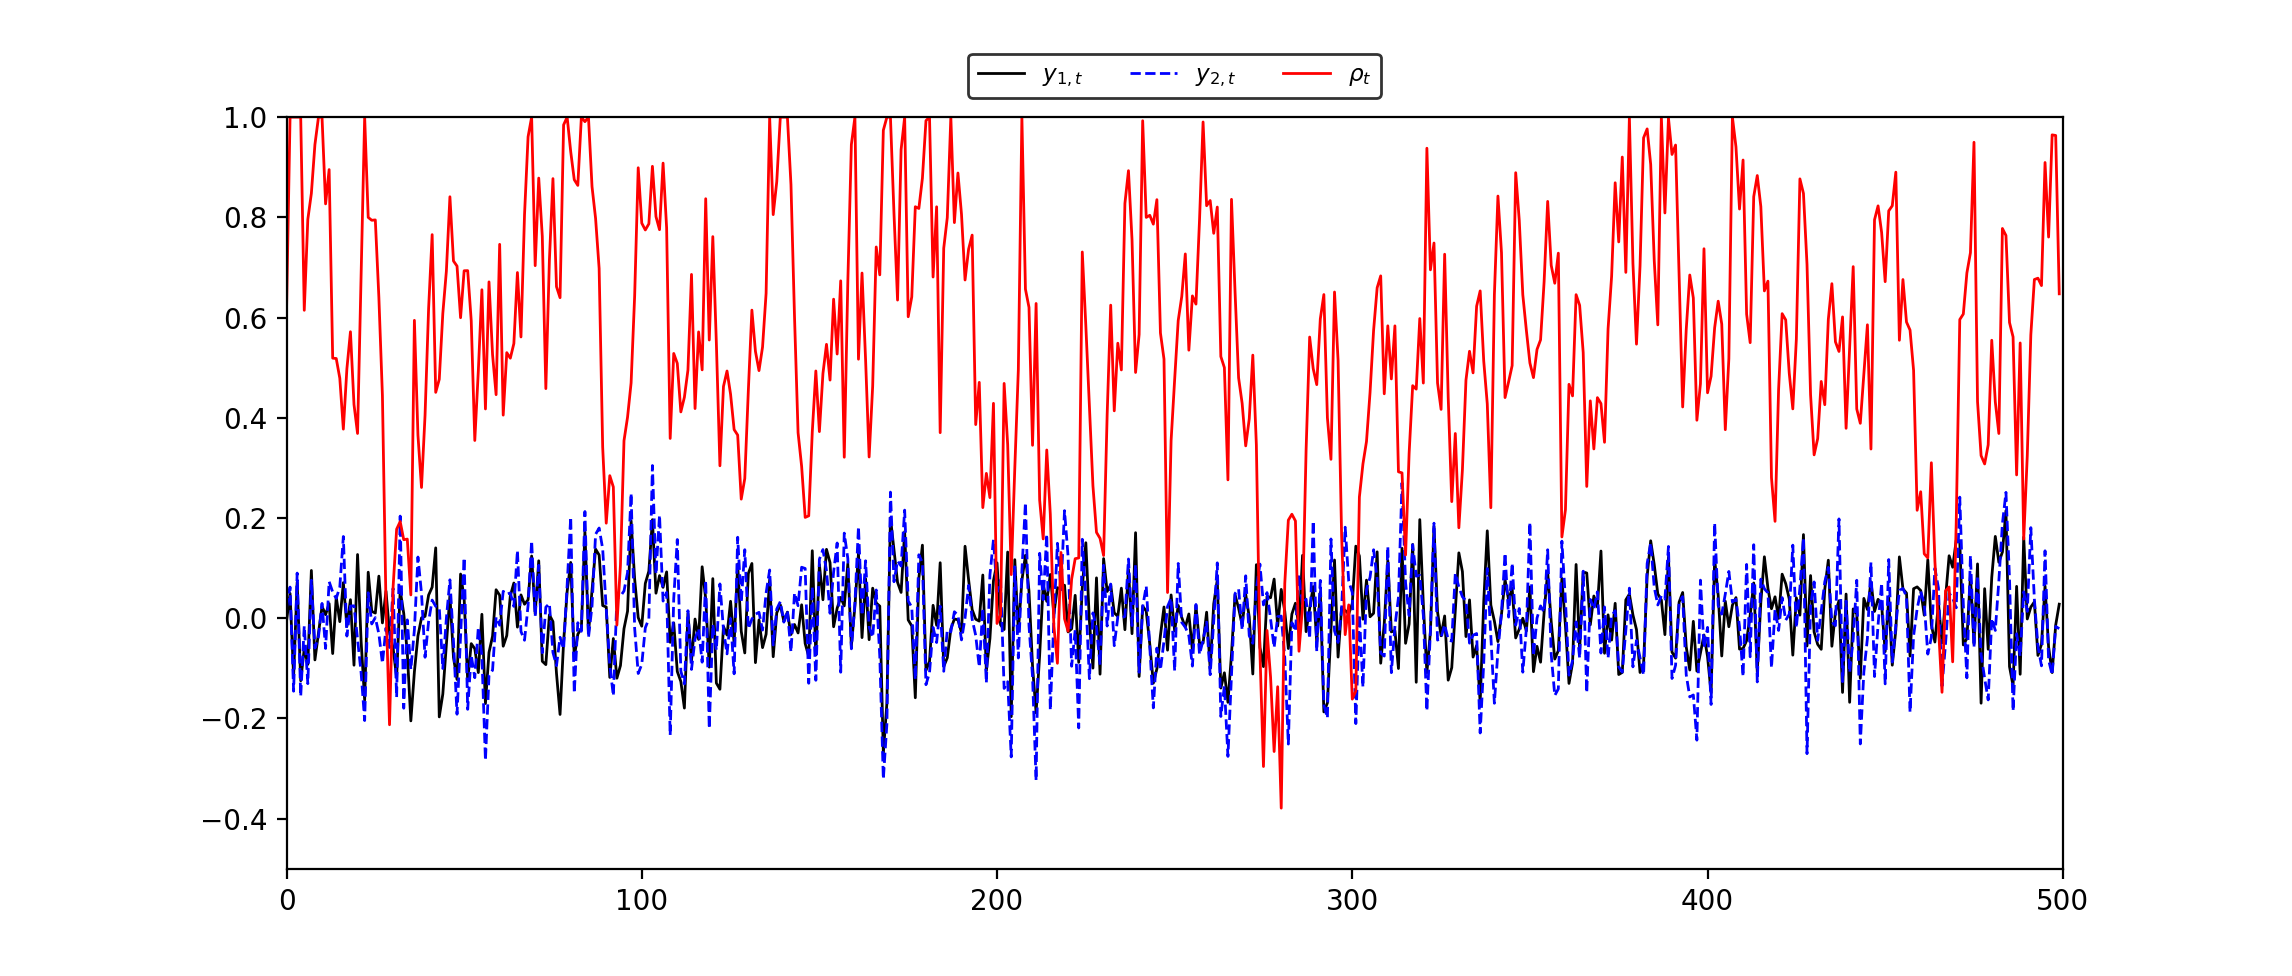
\includegraphics[scale=0.6]{simulation_assetpaths_with_stochastic_correlations.png}
	\caption[Simulated data with time-varying correlation.]{Simulated data and time-varying correlation from \eqref{eq:correlation_simulation}.}
	\label{fig:cholesky_simulation}
\end{figure}

\noindent
Estimation uncertainty associated to estimated correlation coefficients when sample correlations are used as proxy for true correlation in our supervised learning problem will be denoted by the width of their $100(1-\eta)\%$ confidence intervals. These confidence intervals are estimated by application of a bootstrap resampling procedure with replacement: For all time units $t = \{\Delta t, \Delta t +1, \dots, T\}$, for $\Delta t = \{3, 4, \dots, 100\}$, a $1000$ samples of size $\Delta t$ have been randomly selected. For each subsample the correlation coefficient is estimated and, subsequently, the width of the $100(1-\eta)\%$  confidence interval is measured for each coefficient. The parameter $\eta$ is set to $0.01$ in this part of the analysis.    \\ 




\section{Moving Window Estimates of Correlation} \label{sec:MW}
The accuracy of Pearson and Kendall estimates for conditional correlation is compared on the basis of mean squared error (MSE) between estimated and true correlations. The variance of mean squared errors from Pearson estimates in Figure \ref{fig:mse_pearson_kendall_bootstrap} is approximately 1.78e-3 while that of Kendall is approximately 1.59e-3; Kendall estimates seem slightly less sensitive to the choice of window length compared to Pearson estimates but the difference seems negligible small or might even not be significant. Interestingly, it is observed that Kendall estimates for conditional correlation have slightly higher MSE values for larger window lengths. A possible explanation for this observation is that the simulated asset returns follow a multivariate normal distribution, i.e. an elliptical distribution. Therefore, it makes sense that a linear correlation coefficient such as Pearson results in lower MSE values for most window lengths. Pearson can get unreliable in the presence of fat-tailed distributions, which is generally a property of real asset return data \citep{ref:Pozzi2012}. It will be interesting to verify whether Kendall is a better choice for approximation of true correlation in the case of real asset return data in chapter \ref{chap:multivariate_analysis}. \\

\clearpage 

\noindent
Pearson and Kendall moving window estimates of conditional correlation satisfy the positive semidefiniteness condition in the conditional correlation matrix $R_t$ for the entire out-of-sample period under all choices of window length. Figure \ref{fig:det_pearson_kendall} presents the obtained minimum determinants of $R_t$ for all choices of window length. In fact, \cite{ref:Pozzi2012} prove that Pearson and Kendall sample correlations using moving windows yield positive semidefinite correlation matrices.     


\begin{figure}[H]
	\centering
	\begin{subfigure}[b]{0.49 \textwidth}
		\centering 
		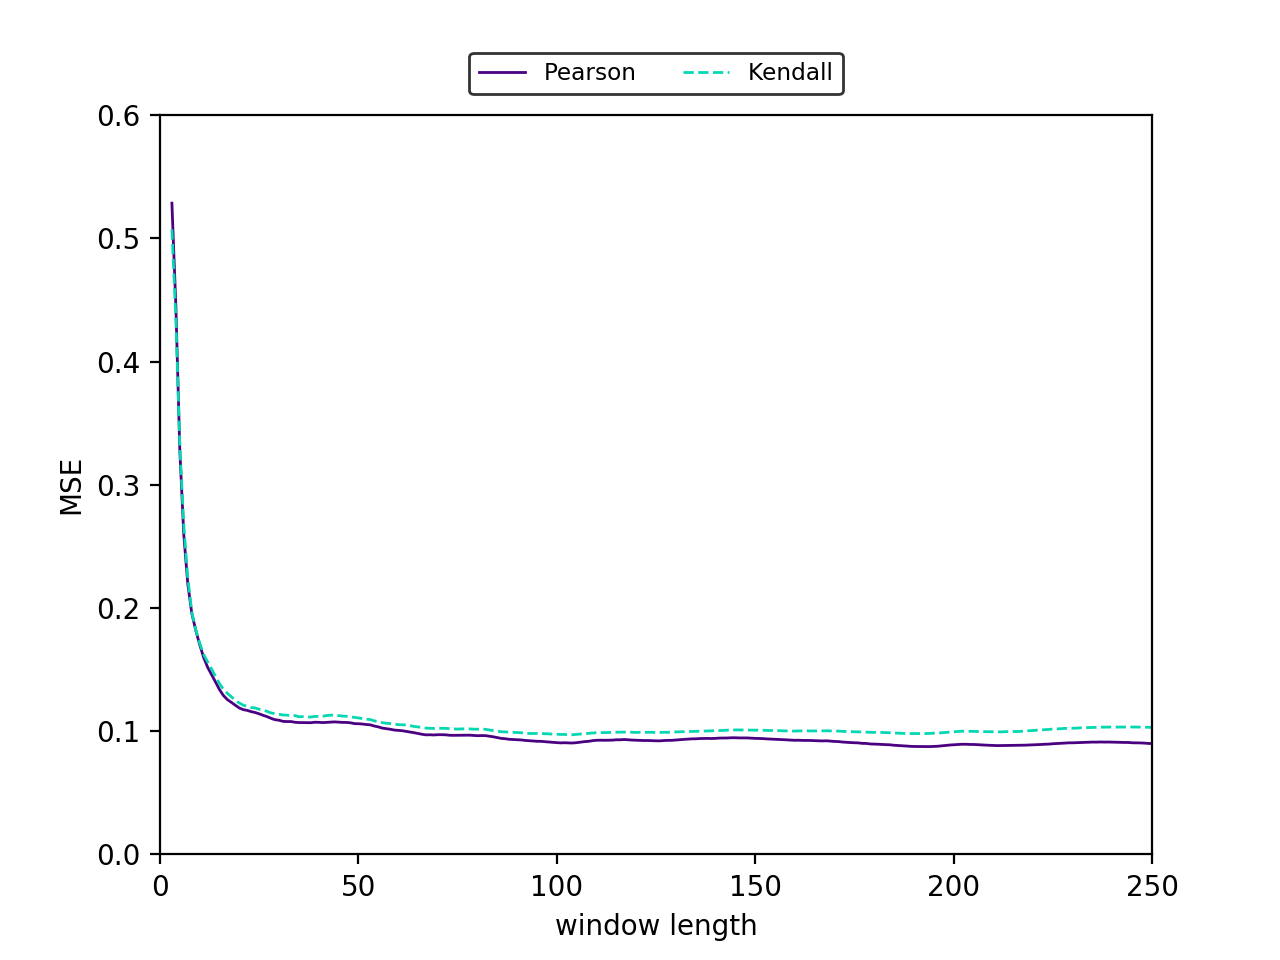
\includegraphics[width=\textwidth, height=0.5\textwidth]{mse_pearson_kendall.png} 
		\caption{MSE for Pearson and Kendall Moving Window bootstrap estimates.}
		\label{fig:mse_pearson_kendall_bootstrap}
	\end{subfigure}
	\begin{subfigure}[b]{0.49 \textwidth}
		\centering 
		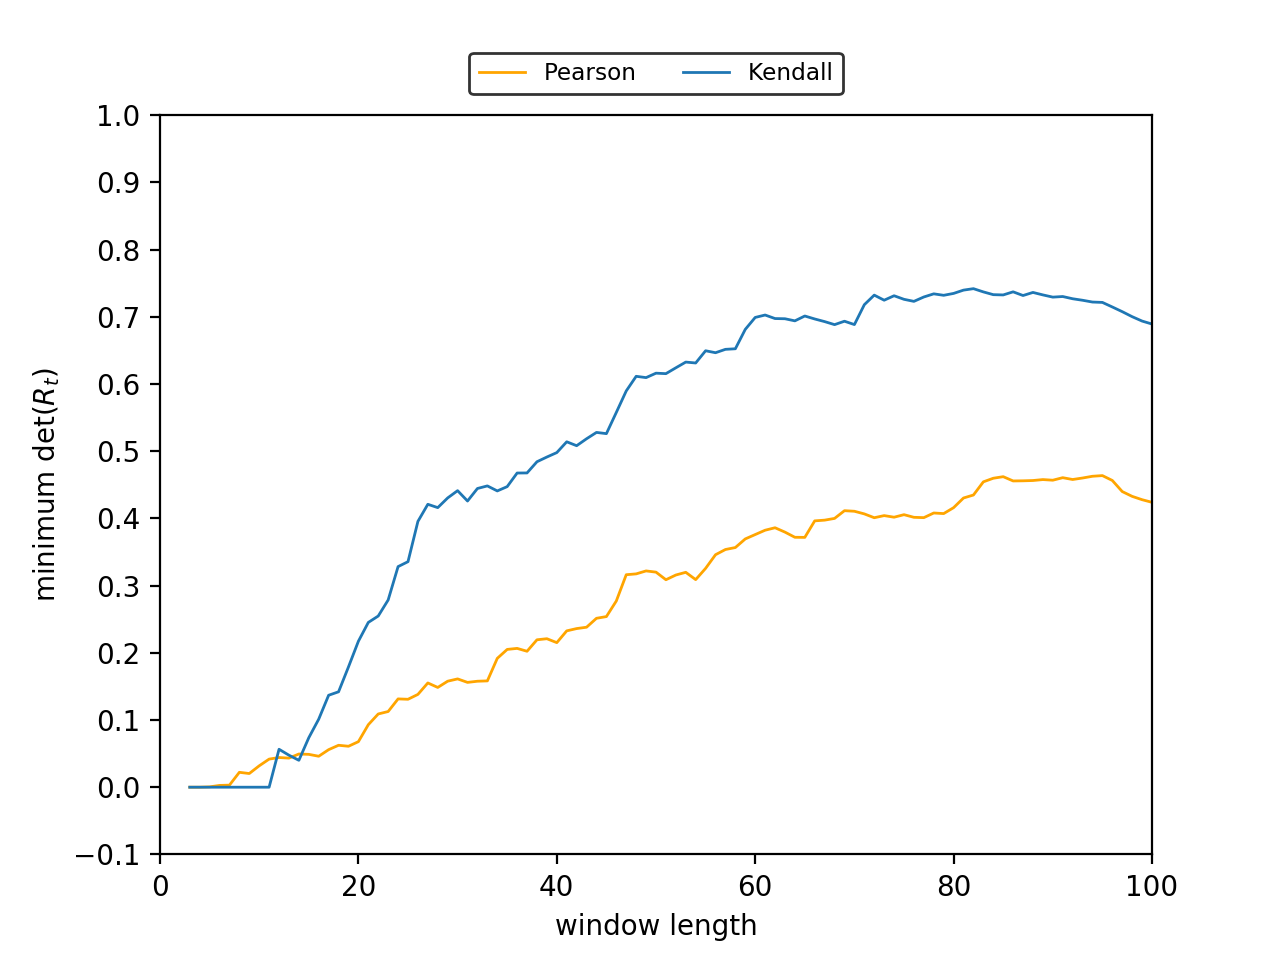
\includegraphics[width=\textwidth, height=0.5\textwidth]{det_pearson_kendall} 
		\caption{Minimum det($R_t$) from Pearson and Kendall Moving Window bootstrap estimates.}
		\label{fig:det_pearson_kendall}
	\end{subfigure}
	\caption[MSE and minimum determinants for Pearson and Kendall Moving Window bootstrap estimates.]{Comparison MSE and minimum determinants for Pearson and Kendall Moving Window bootstrap estimates\protect\footnotemark.}
	\label{fig:mse_det_pearson_kendall_bootstrap}
\end{figure}


\footnotetext{For Pearson and Kendall correlation approximation using moving window estimates with window sizes 3 through 7 several bootstrapped samples return a standard deviation of zero. This results into NaN values for the associated estimated correlation coefficient as the covariance is divided by zero. These NaN values are excluded for calculation of the mean estimate of Pearson and Kendall correlation coefficient over the test set.} 

\noindent
Figure \ref{fig:pearson21_bootstrap} and Figure \ref{fig:kendall21_bootstrap} show that both Pearson and Kendall moving window estimates of correlation change substantially over time indicating the capture of changing correlation levels. Additionally, it is observed that the obtained 99\% confidence intervals around these estimates are rather wide, covering all values in the range $[-1,1]$, which imply that the uncertainty around the estimated values are high \citep{ref:Basturk2016}. Pearson estimates appears to be more volatile than Kendall estimates of correlation, which may be attributed to Kendall's $\tau$ rank correlation's desirable property of being robust to outliers.  \\

\noindent
Furthermore, Pearson and Kendall estimates using moving windows are very sensitive to the choice of the window length. This is illustrated by the bias-variance decomposition of the MSE between estimated and true correlations shown in figures \ref{fig:decom_mse_pearson}-\ref{fig:decom_mse_kendall}. One can observe an inverse relationship between the choice of window length, that is, the bootstrap sample size, and value of the variance term in the MSE decomposition. This relationship may be explained by the fact that as the bootstrap sample size increases with an increase of the window length, the standard error, or the standard deviation of the sampling distribution, decreases. In other words, as the bootstrap sample size increases, the variability of the sampling distribution decreases which would show through smaller 99\% confidence intervals. Figures \ref{fig:decom_mse_pearson}-\ref{fig:decom_mse_kendall} shown this through a decrease in de variance term of the bias-variance decomposition of the MSE between estimated and true correlations. \\

\begin{figure}[H]  % [h] parameter makes sure figures are located at 'this' location.
	\centering
	\begin{subfigure}[b]{0.49 \textwidth} % sum of widths should be less than text width if all one the same line
		\centering 
		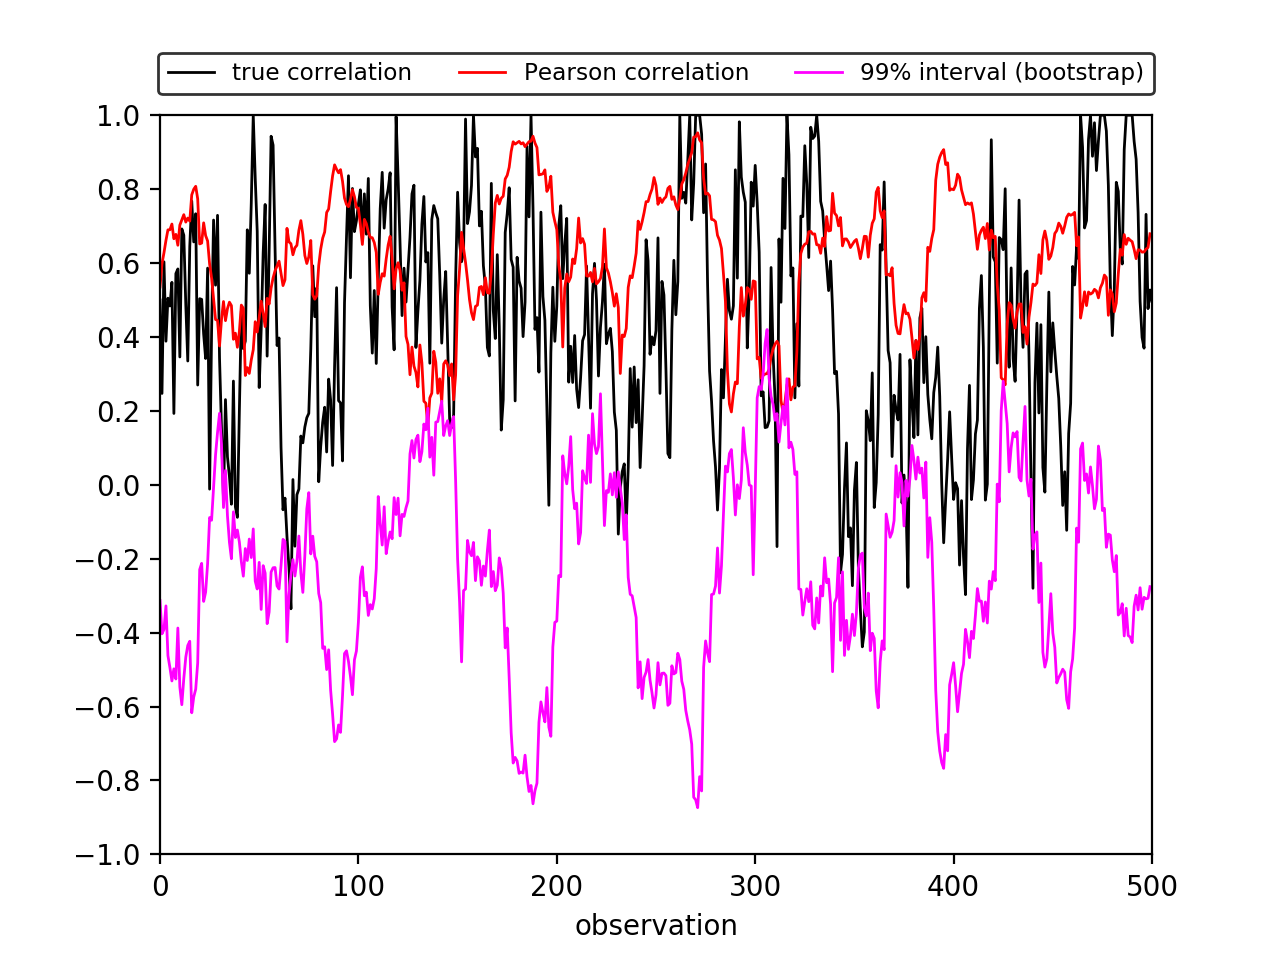
\includegraphics[width=\textwidth, height=0.5\textwidth]{pearson_21_estimates_bootstrap.png} 
		\caption{Pearson estimates with $\Delta_t = 21$.} 		
		\label{fig:pearson21_bootstrap}
	\end{subfigure} 
	\hfill
	\begin{subfigure}[b]{0.49 \textwidth}
		\centering 
		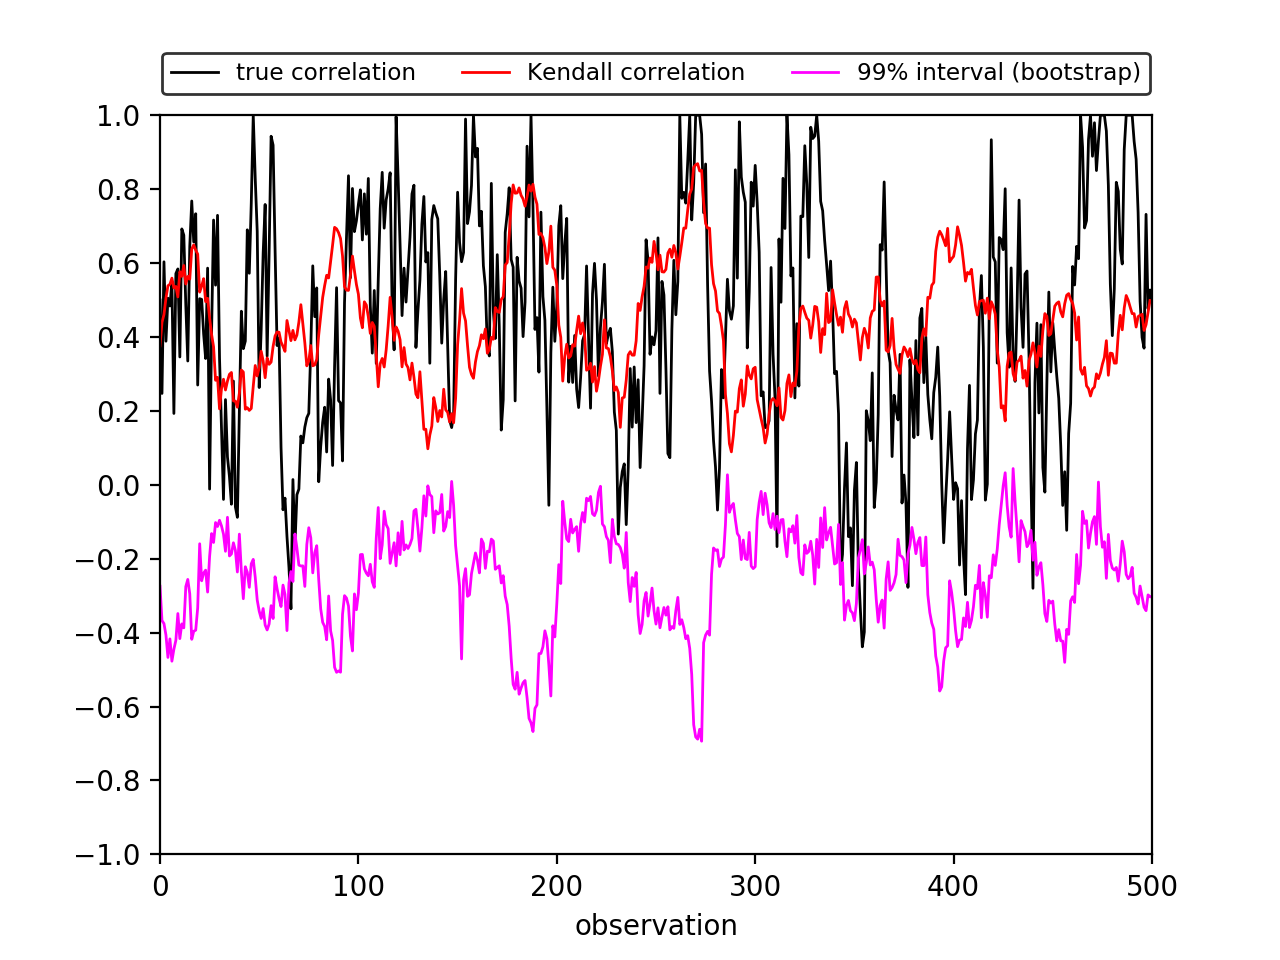
\includegraphics[width=\textwidth, height=0.5\textwidth]{kendall_21_estimates_bootstrap.png} 
		\caption{Kendall estimates with $\Delta_t = 21$.} 		
		\label{fig:kendall21_bootstrap}
	\end{subfigure}
	\hfill
	\begin{subfigure}[b]{0.49 \textwidth} 
		\centering
		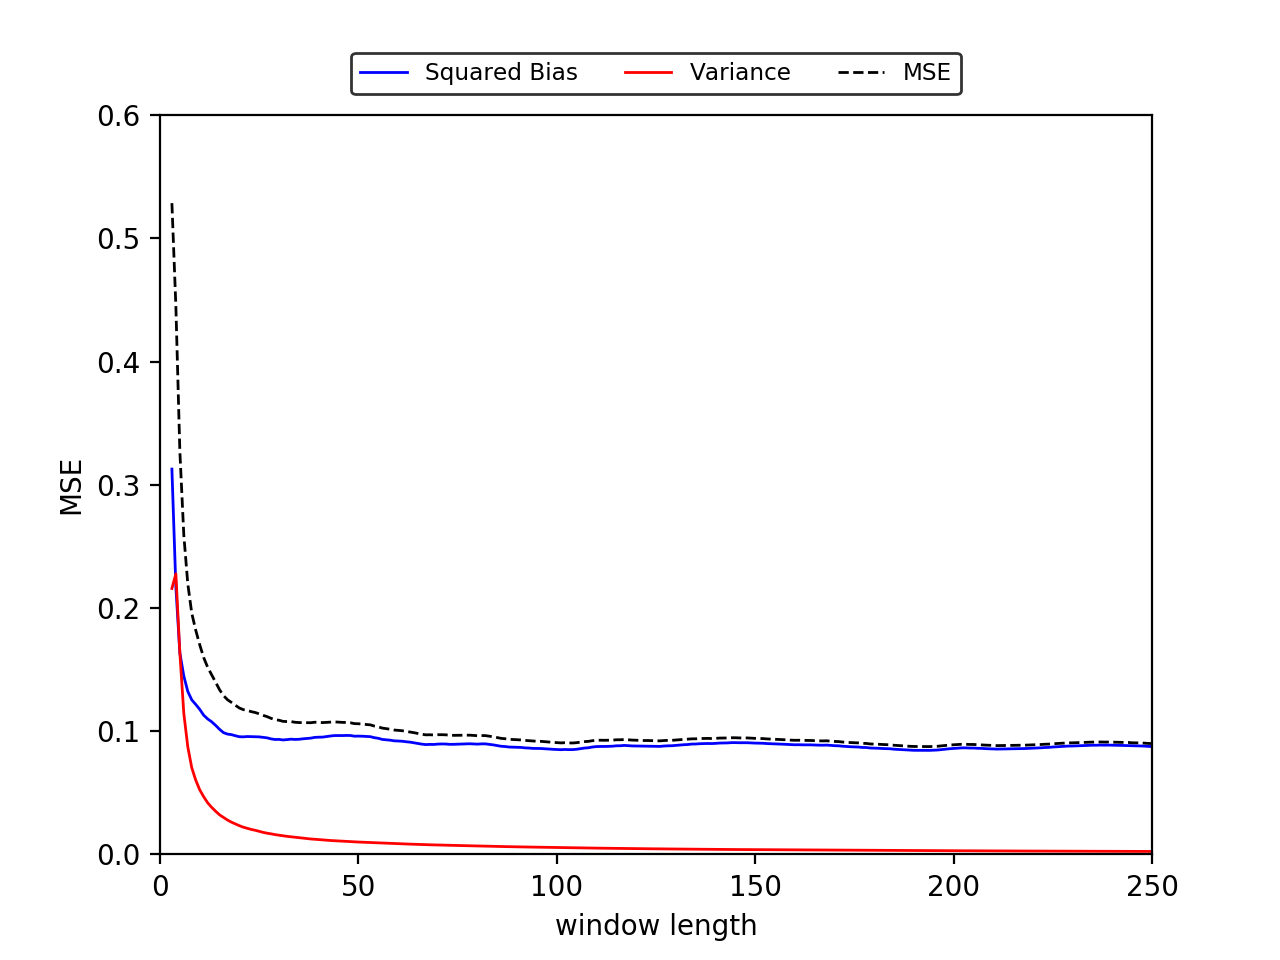
\includegraphics[width=\textwidth, height=0.5\textwidth]{decom_mse_pearson.png}
		\caption{Bias-variance decomposition for Pearson estimates.}
		\label{fig:decom_mse_pearson}
	\end{subfigure}
	\hfill
	\begin{subfigure}[b]{0.49 \textwidth} 
		\centering
		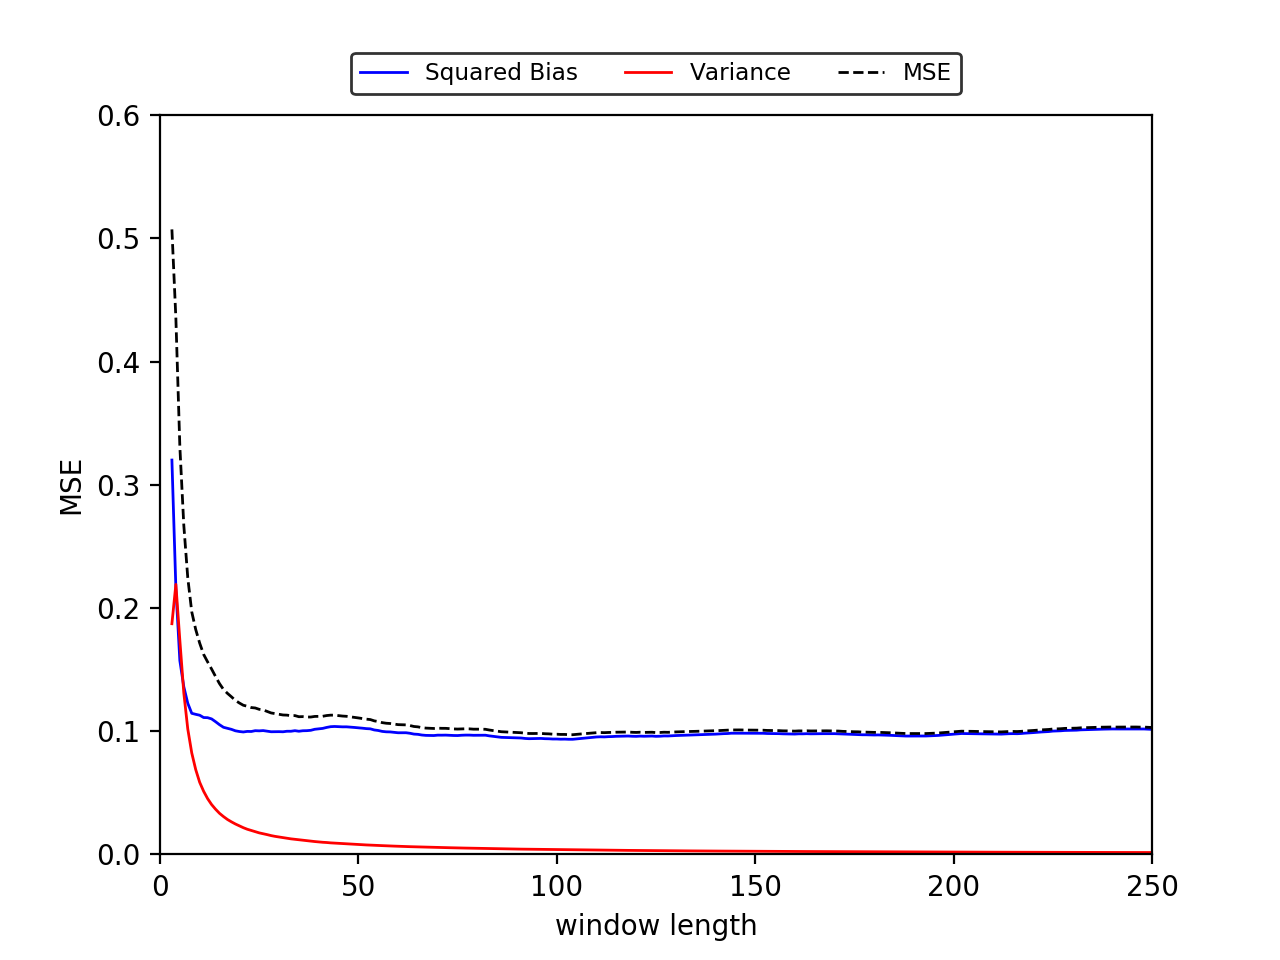
\includegraphics[width=\textwidth, height=0.5\textwidth]{decom_mse_kendall.png}
		\caption{Bias-variance decomposition for Kendall estimates.}
		\label{fig:decom_mse_kendall}
	\end{subfigure}
	\caption{MSE decomposition for Pearson and Kendall Moving Window bootstrap estimates.}
	\label{fig:decom_mse_pearson_kendall_true}
\end{figure}



\section{Learning with True Correlation for Response Variable} \label{sec:true_correlation}
In this section, the covariates of proposed nonparametric learning estimators are approximations of true correlation. The response variable is specified as the true correlation defined by the simulation parameters in \eqref{eq:correlation_simulation}. Using simulation it is possible to study the effect of using approximations of correlations as covariates on the loss function, that is, the mean squared error. One comment on notation: KNN($neighbors=k$) denotes a k-nearest neighbor estimator with $k$ number of neighbors used for estimation of the response variable. Similarly, RF($trees=b$) denotes a random forest estimator with $d$ decision trees defining the random forest. \\


%%%%%% NEAREST neighbor TRUE COR %%%%%%%%
\subsection{Generalization Error of Nearest Neighbor under True Correlation} \label{sec:MSE_knn_true}
The accuracy of KNN estimates with Pearson and Kendall covariates for conditional correlation is compared in terms of the MSE between estimated and true correlations. Figure \ref{fig:mse_knn5_pearson_kendall_true} depicts MSE from KNN(5) with Pearson and Kendall moving window estimates of correlation for covariates. Regardless of the choice of window length, MSE from KNN(5) with Pearson and Kendall covariates are between 0.0939 and 0.1071, and 0.0929 and 0.1071, respectively. The variance of MSE from KNN(5) estimates with Pearson covariates is approximately 6.07e-6 while that of KNN estimates with Kendall covariates is approximately 5.66e-6. KNN thus appears to be insensitive to the choice of window length, regardless whether the set of covariates is constructed from Pearson or Kendall moving window estimates of correlation. KNN's property of insensitivity to the choice of window length is preferred over Pearson and Kendall's property of being highly sensitive to the choice of the window length used for correlation estimates as depicted in figure \ref{fig:mse_pearson_kendall_bootstrap}. Moreover, KNN(5) estimates of conditional correlation satisfy the positive semidefiniteness condition in the conditional correlation matrix $R_t$ for the entire out-of-sample period under all choices of window length. Figure \ref{fig:det_knn5_pearson_kendall_true} presents the obtained minimum determinants of $R_t$ for all choices of window length.  
     
\begin{figure}[H]
	\centering
	\begin{subfigure}[b]{0.49 \textwidth} 
		\centering
		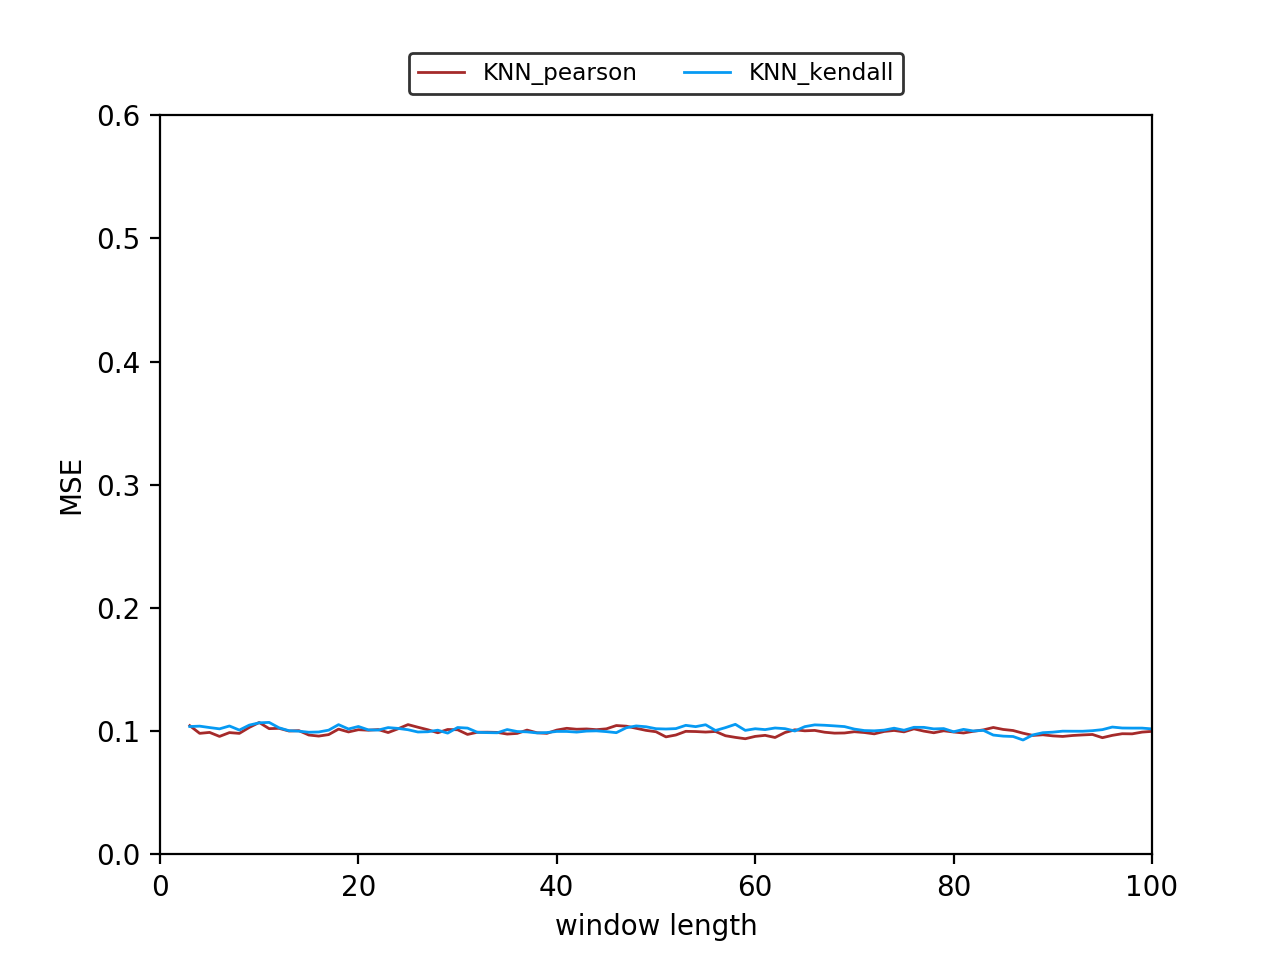
\includegraphics[width=\textwidth, height=0.5\textwidth]{mse_knn5_pearson_kendall_true.png}
		\caption{MSE for KNN(5) with covariates from Pearson and Kendall and true correlation.}
		\label{fig:mse_knn5_pearson_kendall_true}
	\end{subfigure}
	\hfill
	\begin{subfigure}[b]{0.49 \textwidth} 
		\centering
		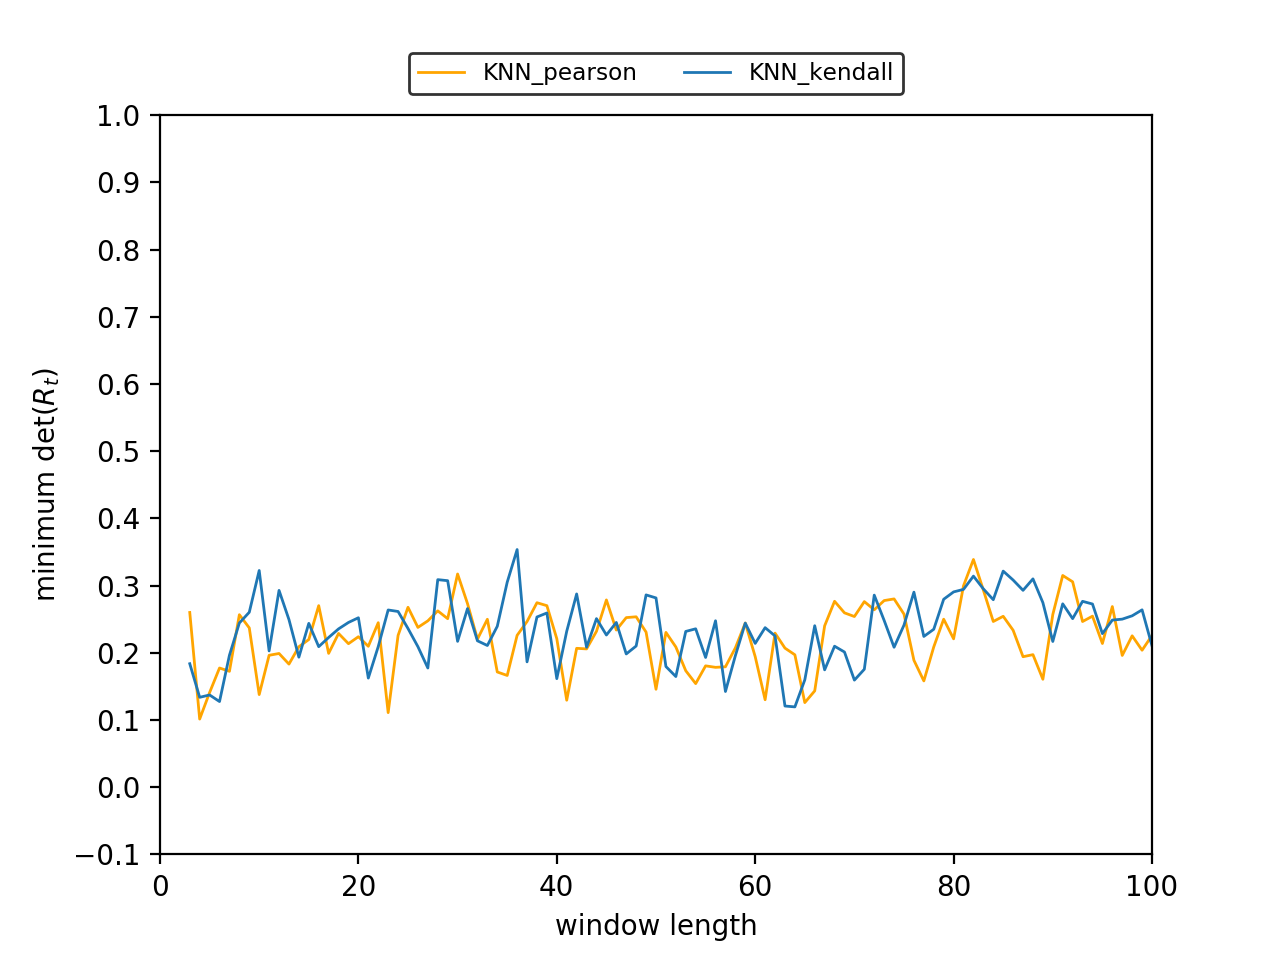
\includegraphics[width=\textwidth, height=0.5\textwidth]{det_knn5_pearson_kendall_true.png}
		\caption{Minimum determinants for KNN(5) with covariates from Pearson and Kendall and true correlation.}
		\label{fig:det_knn5_pearson_kendall_true}
	\end{subfigure}
	\caption[MSE and minimum determinants for KNN(n\_neighbors=5) under true correlation.]{Comparison MSE and minimum determinants for KNN(n\_neighbors=5) with covariates from Pearson and Kendall and true correlation.}
	\label{fig:mse_det_knn5_pearson_kendall_true}
\end{figure}


\noindent
From visual inspection of the plots in Figure \ref{fig:knn_pearson21_bootstrap_true} and Figure \ref{fig:knn_kendall21_bootstrap_true} it seems that the uncertainty in the conditional correlation, $\rho_t$, which is illustrated by the $99\%$ confidence interval, is smaller for KNN estimates compared to Pearson and Kendall moving window estimates under the same window length of 21 days. KNN(5) estimates of correlation are, however, much more volatile. This may be a less desirable result as it is not expected that correlation between assets changes that drastically at each time unit. Rather, correlation is expected to vary gradually over time \citep{ref:Basturk2016}. It is observed though that, as with an increase in window length for Pearson and Kendall moving window estimates of correlation, an increase in the number of neighbors results in smoother KNN estimates of correlation. \\

\noindent
Figures \ref{fig:decom_mse_knn5_pearson_true}-\ref{fig:decom_mse_knn5_kendall_true} present the MSE decomposition into bias and variance terms for KNN(5) estimates of correlation. These figures indicate that the KNN estimator is considerably less sensitive to the choice of the window length for smaller window sizes when compared to Pearson and Kendall sample correlations using moving windows. The uncertainty around the estimated correlations appears to be marginally affected by the choice of the window length for all window sizes. This statement is supported by the fact that the variance as a function of the window length behaves like a (more or less) constant red line in these figures.   

\begin{figure}[H]  % [h] parameter makes sure figures are located at 'this' location.
	\centering
	\begin{subfigure}[b]{0.49 \textwidth} % sum of widths should be less than text width if all one the same line
		\centering 
		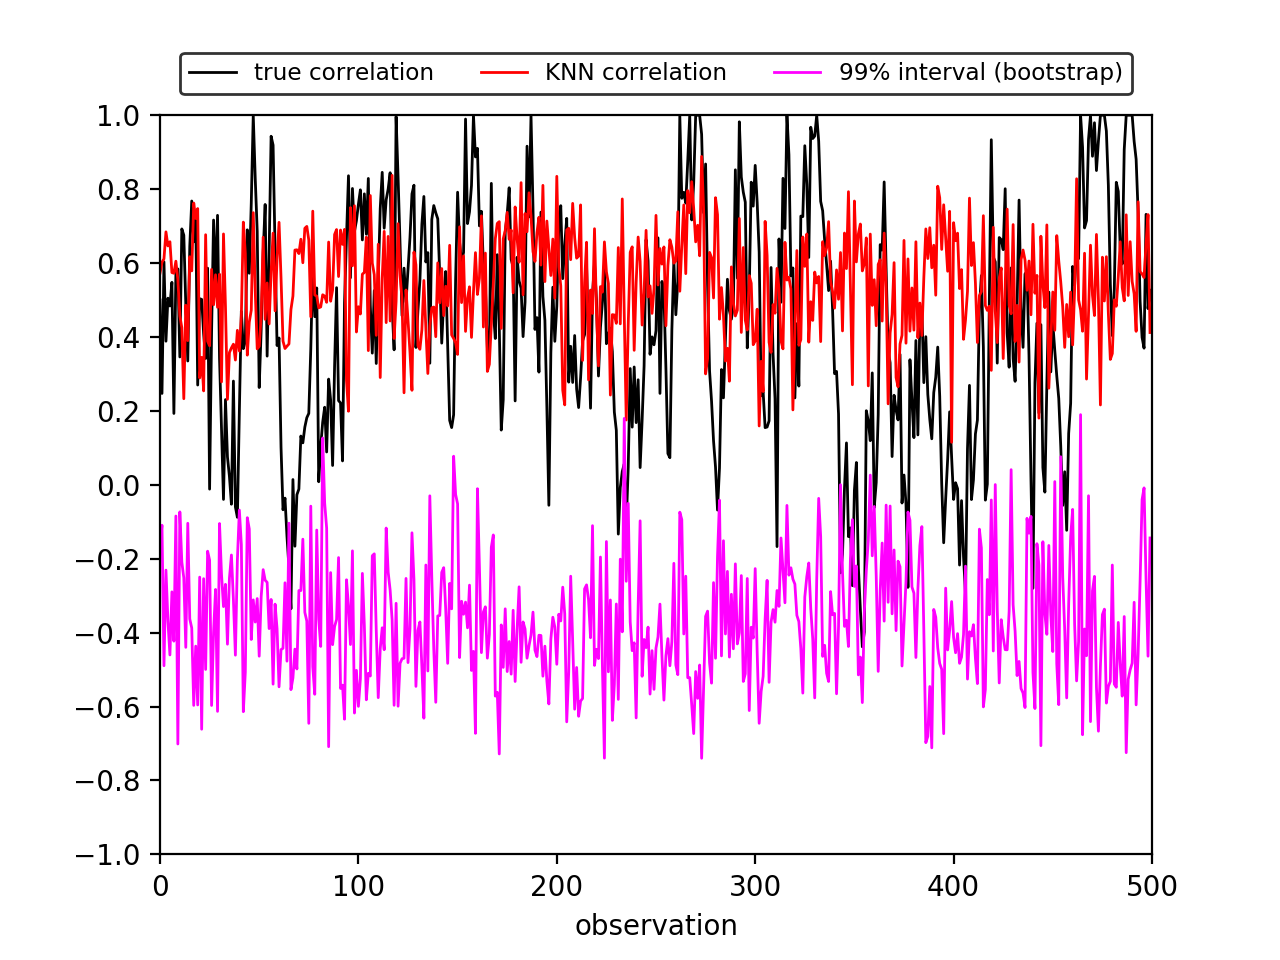
\includegraphics[width=\textwidth, height=0.5\textwidth]{knn_pearson_21_estimates_bootstrap_true.png} 
		\caption{KNN(5) estimates with $\Delta_t = 21$, Pearson as covariate and true correlation.} 	
		\label{fig:knn_pearson21_bootstrap_true}
	\end{subfigure} 
	\hfill	
	\begin{subfigure}[b]{0.49 \textwidth} 
		\centering 
		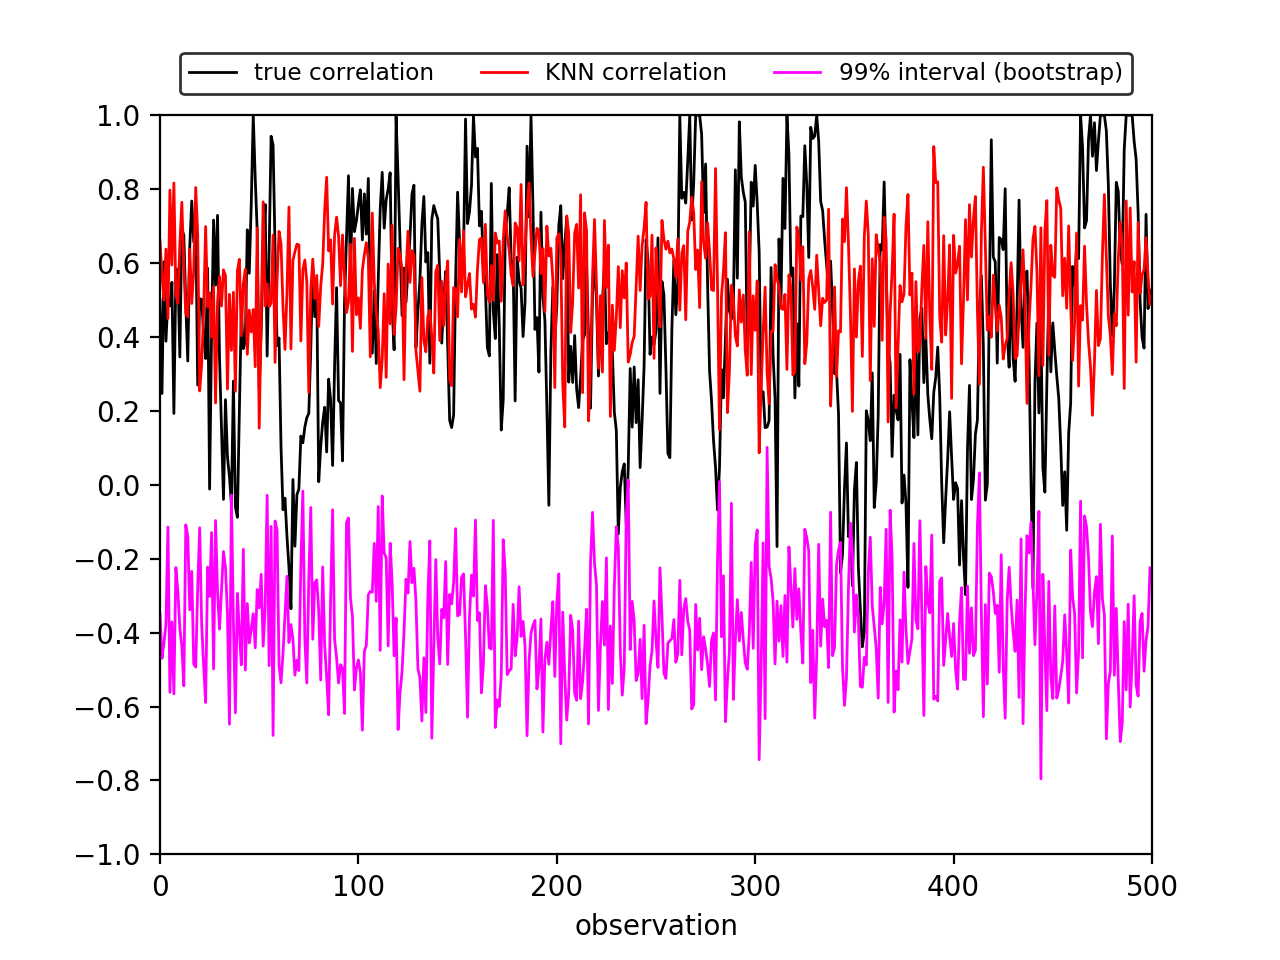
\includegraphics[width=\textwidth, height=0.5\textwidth]{knn_kendall_21_estimates_bootstrap_true.png} 
		\caption{KNN(5) estimates with $\Delta_t = 21$, Kendall as covariate and true correlation.} 
		\label{fig:knn_kendall21_bootstrap_true}
	\end{subfigure} 
	\hfill	
	\begin{subfigure}[b]{0.49 \textwidth}
		\centering 
		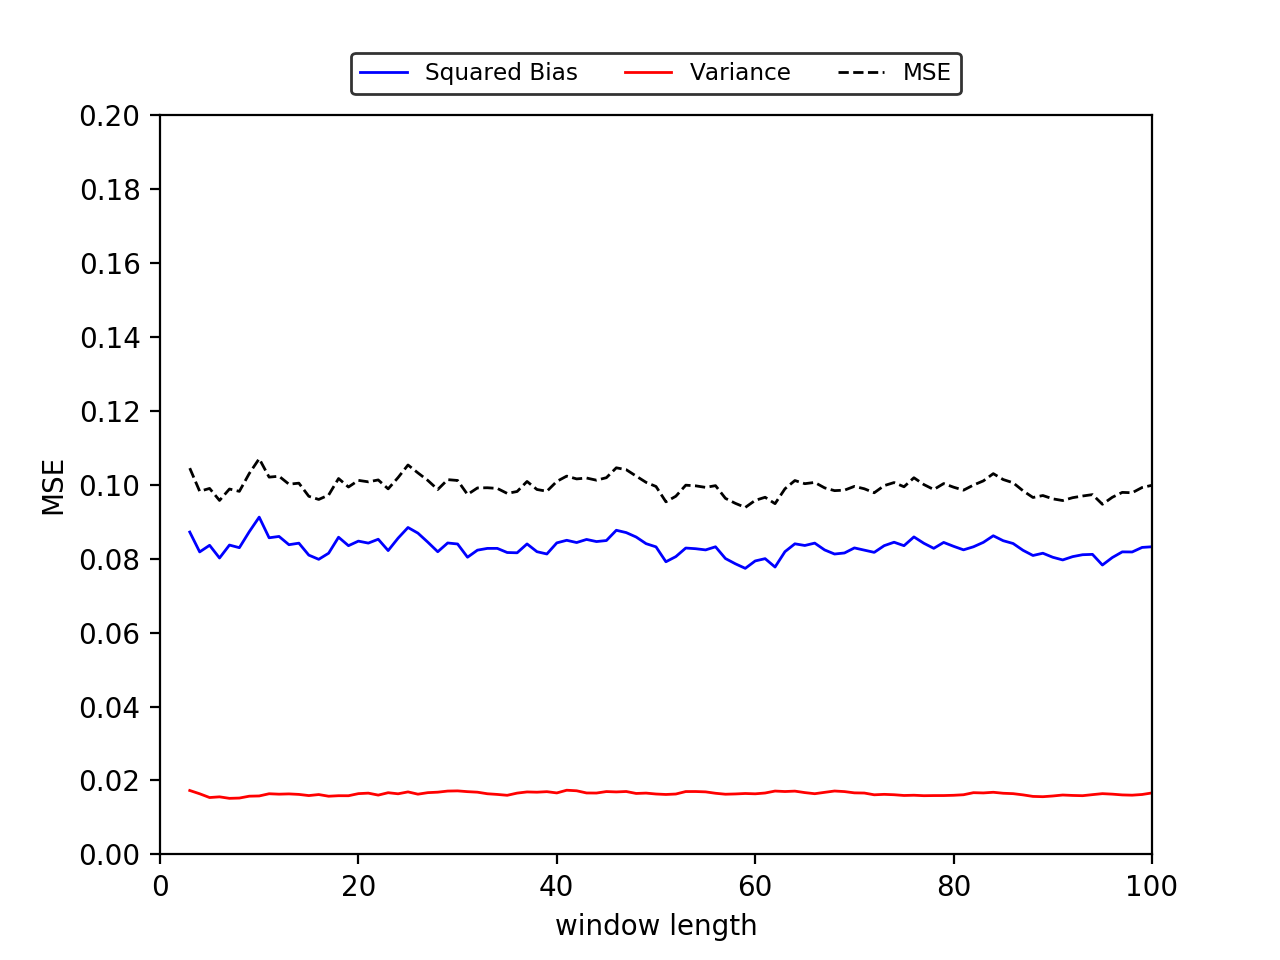
\includegraphics[width=\textwidth, height=0.5\textwidth]{decom_mse_knn5_pearson_true.png} 
		\caption{Bias-variance decomposition for KNN(5) estimates with Pearson as covariate and true correlation.} 	
		\label{fig:decom_mse_knn5_pearson_true}
	\end{subfigure}
	\hfill  
	\begin{subfigure}[b]{0.49 \textwidth}
		\centering 
		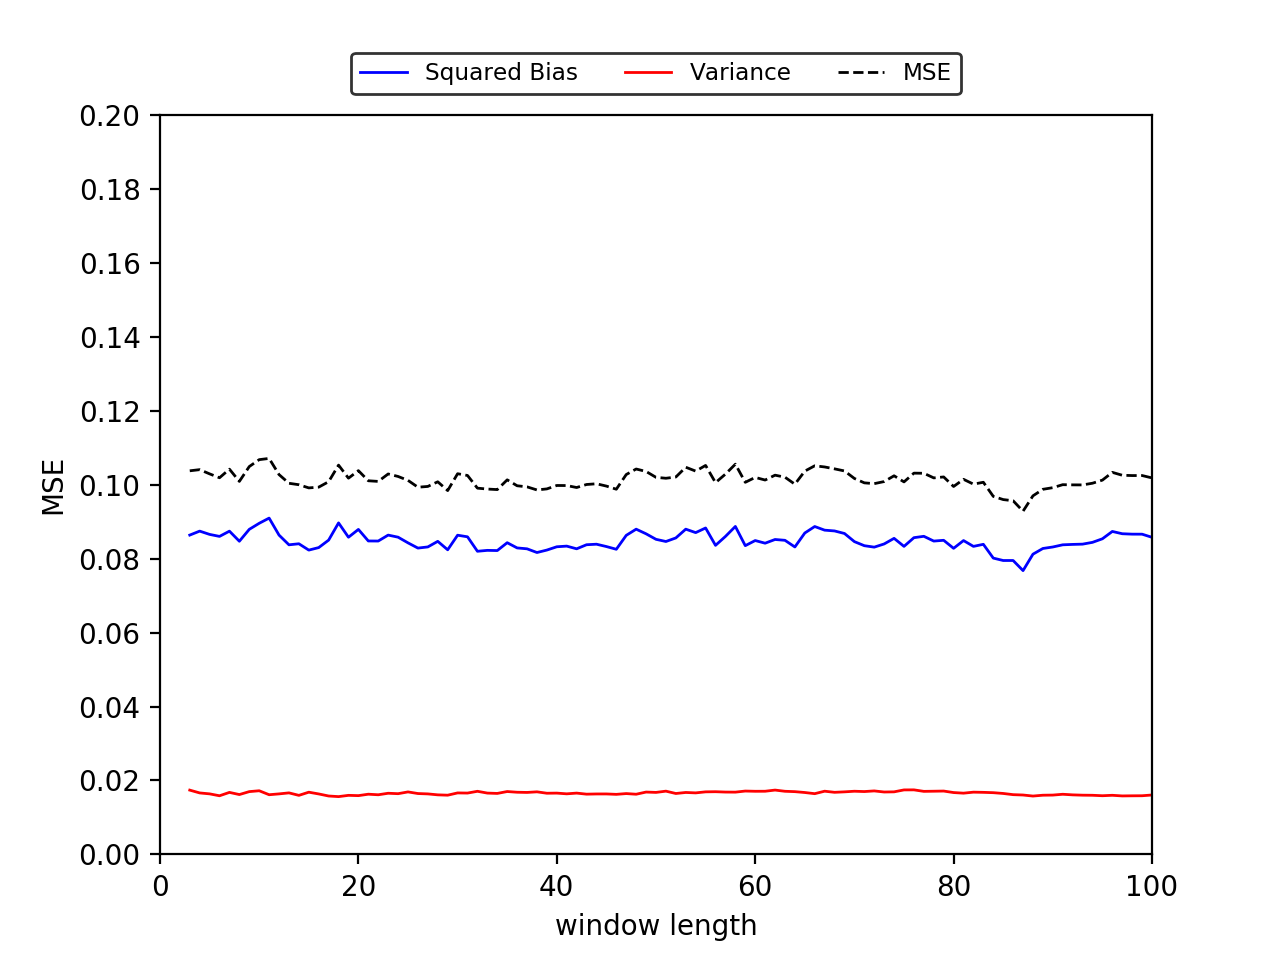
\includegraphics[width=\textwidth, height=0.5\textwidth]{decom_mse_knn5_kendall_true.png} 
		\caption{Bias-variance decomposition for KNN(5) estimates with Kendall as covariate and true correlation.} 
		\label{fig:decom_mse_knn5_kendall_true}
	\end{subfigure}
	\caption[MSE decomposition for KNN(5) estimates under true correlation.]{MSE for KNN(5) estimates with Pearson and Kendall Moving Window bootstrap estimates as covariates and true correlation.}
	\label{fig:decom_mse_knn5_pearson_kendall_true}
\end{figure}

\subsection{Effect of Alternative Nearest Neighbor Parameterizations under True Correlation} \label{sec:MSE_knn_alt_true}
Figure \ref{fig:decom_mse_pearson_kendall_true} depicted an inverse relationship between the window length and the uncertainty around Pearson and Kendall sample correlation estimates using moving windows. The KNN estimator has a similar property: simulation results in tabel \ref{tab:mse_decomp_knn_pearson_kendall_true} show an inverse relationship between the number of nearest neighbors used in the estimation of correlations and the uncertainty around the estimated correlations, regardless whether Pearson or Kendall estimates are used for specification of the set of covariates. It is clearly observed that an increase in the number of neighbors $k$ results in a decrease of the variance, and conversely. This observation is in line with our discussion on MSE decomposition for the KNN estimator in section \ref{sec:mse_decompose}. Furthermore, it was stated that the higher the value of $k$, the lower the model complexity and, as such, the squared bias tends to increase with an increase in $k$. However, simulation results depicted in tabel \ref{tab:mse_decomp_knn_pearson_kendall_true} indicate no increase in squared bias with an initial increase in $k$. The first increase in squared bias is observed when the $k$ is approximately 900. For all $k$ smaller than 900 a decrease in squared bias is observed with an increase in $k$. This statement is more clearly shown through a visual representation of the MSE decomposition as a function of the number of neighbors for $k \in \{5, 10, 25, 50, 100\}$ in figure \ref{fig:knn5_pearson_kendall_sens_analysis_true}. \\  


%% TABLE
\begin{table}[H]
\centering
\captionsetup[subtable]{position=below}
%\captionsetup[table]{position=below}
\begin{subtable}{0.49\linewidth}
\centering
\begin{tabular}{r  c  c  c} 
\toprule
\multicolumn{1}{ r }{\textbf{k}} &
\multicolumn{1}{ c }{\textbf{Squared Bias}} &
\multicolumn{1}{ c }{\textbf{Variance}} &
\multicolumn{1}{ c }{\textbf{MSE}} \\
\midrule 

5                                     & 0.0913                         & 0.0158                & 0.1071     \\
10                                   & 0.0831                         & 0.0087                & 0.0917     \\
25                                   & 0.0785 	                    & 0.0037                & 0.0821     \\
50                                   & 0.0781                         & 0.0018                & 0.0799     \\
100                                 & 0.0785                         & 9.23e-4               & 0.0794      \\
200                                 & 0.0776                         & 4.62e-4               & 0.0781      \\
400                                 & 0.0768                         & 2.31e-4               & 0.0770      \\
600                                 & 0.0757                         & 1.55e-4               & 0.0759     \\
800                                 & 0.0756                         & 1.18e-4               & 0.0757      \\
900				     & 0.0761			   & 1.06e-4              & 0.0760      \\
1000                               & 0.0767                         &  9.70e-5              & 0.0768     \\ [1ex]
\bottomrule
\end{tabular}
\caption{MSE for KNN estimates with $\Delta_t = 10$, Pearson as covariate and true correlation.}
\label{tab:mse_decomp_knn_pearson_true}
\end{subtable}
\hfill
\begin{subtable}{0.49\linewidth}
\centering
\begin{tabular}{r  c  c  c} 
\toprule
\multicolumn{1}{ r }{\textbf{k}} &
\multicolumn{1}{ c }{\textbf{Squared Bias}} &
\multicolumn{1}{ c }{\textbf{Variance}} &
\multicolumn{1}{ c }{\textbf{MSE}} \\
\midrule 

5                                     & 0.0896                         &  0.0172               & 0.1068   \\
10                                   & 0.0828                         & 0.0092                & 0.0920   \\
25                                   & 0.0764	                   & 0.0038                & 0.0802    \\
50                                   &  0.0749                        & 0.0019               & 0.0769    \\
100                                 & 0.0749                         & 9.47e-4               & 0.0759    \\
200                                 &  0.0753                        & 4.69e-4              & 0.0757    \\
400                                 &  0.0750                        & 2.37e-4              & 0.0752    \\
600                                 & 0.0749                         & 1.59e-4             & 0.0750     \\
800                                 &   0.0750                       & 1.21e-4             & 0.0751     \\
900				     &  0.0757			   & 1.08e-4             & 0.0758     \\
1000                               &  0.0763                        & 9.80e-5             & 0.0764     \\  [1ex]
\bottomrule
\end{tabular}
\caption{MSE for KNN estimates with $\Delta_t = 10$, Kendall as covariate and true correlation.}
\label{tab:mse_decomp_knn_kendall_true}
\end{subtable}
\caption{MSE decomposition as a function of the number of neighbors (k) for KNN with proxy covariates and true correlation.}
\label{tab:mse_decomp_knn_pearson_kendall_true}
\end{table}

\noindent
Figures \ref{fig:knn5_pearson_sens_analysis_true}-\ref{fig:knn5_kendall_sens_analysis_true} depict visual representations of the simulation results for KNN estimates with Pearson and Kendall covariates, respectively. The MSE decomposition as a function of the number of neighbors for $k \in \{5, 10, 25, 50, 100\}$ clearly shows a decrease in the squared bias with an increase in $k$. Given equation \eqref{eq:mse_decomposition_knn} and our discussion from section \ref{sec:mse_decompose} one might have expected an increase in squared bias with an increase in $k$. A possible explanation for the contrasting behavior may be that up to some $k$, an increase in $k$ implies additional neighbors containing informational value are used for the estimation of conditional correlation. Logically, the inclusion of additional neighbors containing informational value results into more accurate estimates of correlation, which shows through a decrease in squared bias. As of some $k$, additional neighbors only add noise to the estimation process which results into increased squared bias.    

\begin{figure}[H]  % [h] parameter makes sure figures are located at 'this' location.
	\centering
	\begin{subfigure}[b]{0.49 \textwidth} % sum of widths should be less than text width if all one the same line
		\centering 
		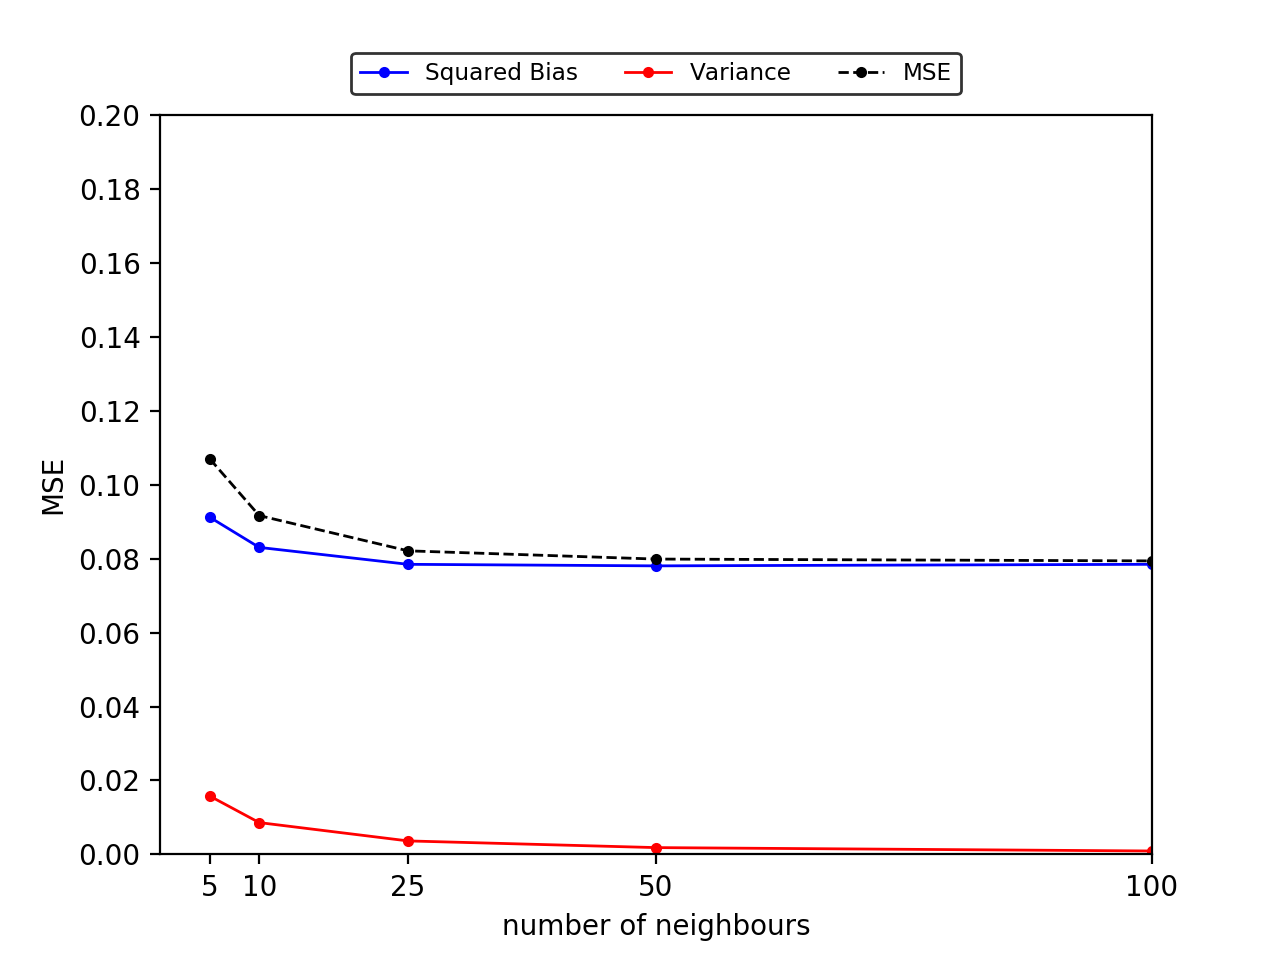
\includegraphics[width=\textwidth, height=0.5\textwidth]{sens_analysis_mse_knn_pearson_true.png} 
		\caption{KNN estimates with $\Delta_t = 10$, Pearson as covariate and true correlation.}
		\label{fig:knn5_pearson_sens_analysis_true}
	\end{subfigure} 
	\hfill	
	\begin{subfigure}[b]{0.49 \textwidth} 
		\centering 
		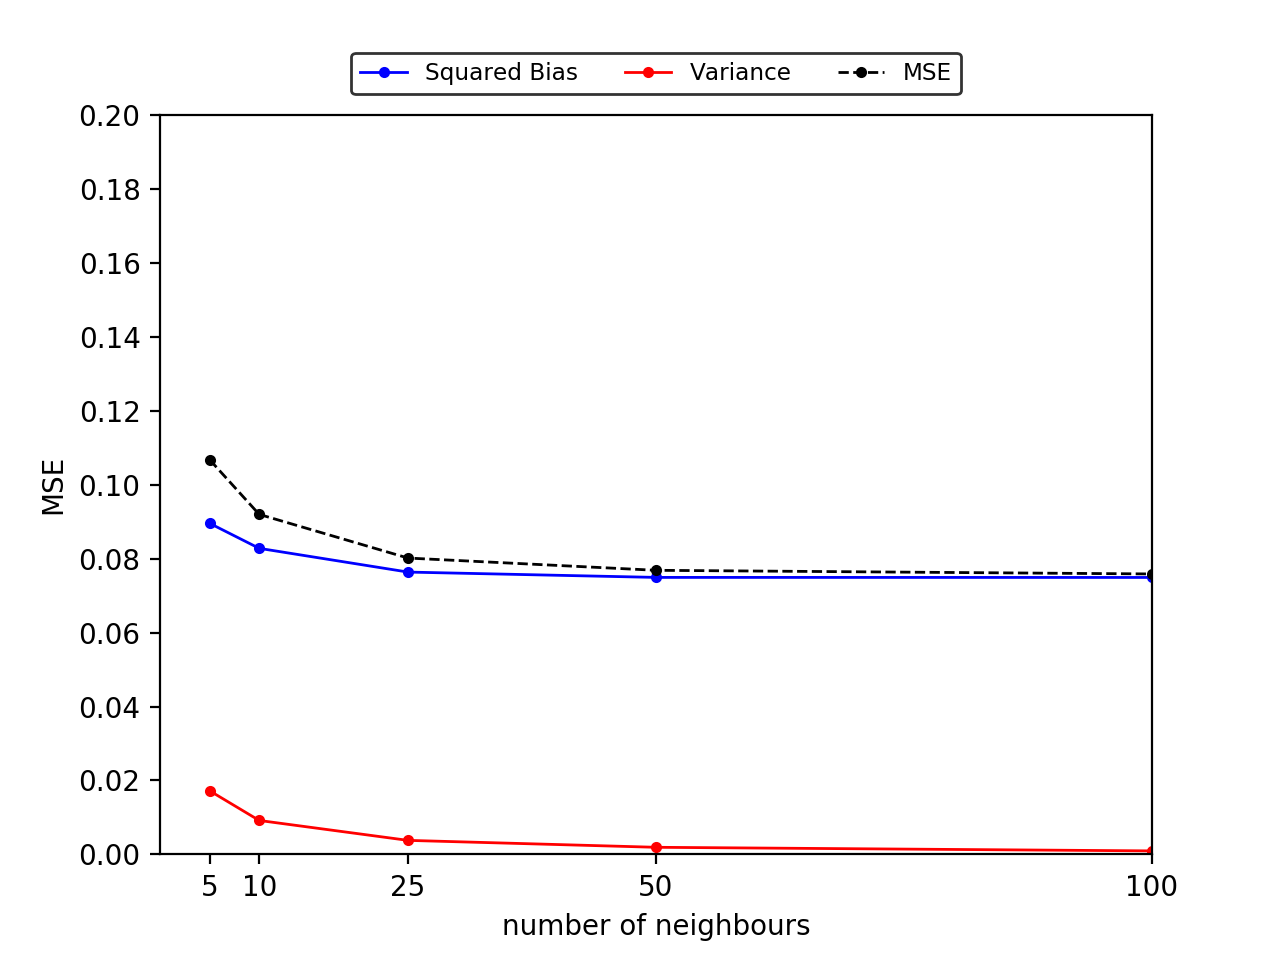
\includegraphics[width=\textwidth, height=0.5\textwidth]{sens_analysis_mse_knn_kendall_true.png} 
		\caption{KNN estimates $\Delta_t = 10$, Kendall as covariate and true correlation.} 
		\label{fig:knn5_kendall_sens_analysis_true}
	\end{subfigure} 
	\caption[MSE as function of number of neighbors for KNN estimates under true correlation.]{MSE as function of number of neighbors for KNN estimates with Pearson and Kendall as covariates and true correlation.}
	\label{fig:knn5_pearson_kendall_sens_analysis_true}
\end{figure}

\clearpage

\noindent
Next, two more parameterizations of the KNN learning algorithm are analyzed. In both parameterizations, the set of neighbors used for point estimation of conditional correlation is defined as the entire training data set. In the first parameterization, the KNN estimator uses an uniformly weighted average of correlations where each of the neighbors contributes equally to the point estimate of conditional correlation, as defined in \eqref{eq:uni_weights}, and will be referred to as KNN(unif). In the second parameterization, the KNN estimator uses an inverse distance weighted average of correlations, as defined in \eqref{eq:inverse_weights}, which will be referred to as KNN(idw). Figure \ref{fig:decom_mse_knn_len_train_IDW_pearson_kendall_true} presents MSE decomposition of both parameterizations with Pearson covariates and true correlation. Clearly, the variance terms become negligible small in case the set of neighbors used for point estimation of conditional correlation is defined as the entire training data set, regardless of the weighting function. The variance, depicted by the red line, is barely observable in the bottom of figures \ref{fig:decom_mse_knn_len_train_pearson_true}-\ref{fig:decom_mse_knn_IDW_pearson_true}. This observation is in line with results depicted in tabel \ref{tab:mse_decomp_knn_pearson_kendall_true} where the value of the variance term is negligible small for a large number of neighbors such as $k=1000$, regardless whether the set of covariates is constructed from Pearson or Kendall moving window estimates of correlation. \\

\noindent
Although low variance is a desirable property of any estimator, the estimated correlation dynamics depicted in figures \ref{fig:decom_mse_knn_len_train_pearson_true}-\ref{fig:decom_mse_knn_IDW_pearson_true} show very little volatility\footnote{Only behavior of the alternative parameterized KNN estimators with Pearson covariates is shown as behavior of its Kendall counterpart is nearly identical.}. In fact, the estimated correlation dynamics of KNN(unif) resemble assuming constant correlation, which is the exact concept we aim to improve on by assuming correlation between financial returns to be time-varying. In case of KNN(idw), the estimator does capture some conditional correlation dynamics resulting in low volatile and smooth correlation dynamics. In practice, the underlying correlation dynamics may potentially be best captured optimizing over the hyperparmeter $k$ until an appropriate level of volatility and smoothness is reached.              \\      

\noindent
Accuracy of the two different parameterizations is compared using MSE between estimated and true correlations. In figure \ref{fig:decom_mse_knn_len_train_pearson_true}, MSE from KNN(unif) is approximately 0.0785, regardless of the choice of window length and whether Pearson or Kendall moving window estimates are use for constructing the set of covariates. In figure \ref{fig:decom_mse_knn_IDW_pearson_true}, MSE from KNN(idw) is approximately between 0.0721 and 0.0774, and between 0.0727 and 0.0771 when Pearson and Kendall moving window estimates are used as covariates, respectively. This implies that slightly lower MSE values are obtained with an inverse distance weighting function as opposed to an uniform weighting function, which is line with our discussion from section \ref{sec:knn}. It makes sense to have training instances with a higher amount of proximity to the input instance contribute more to the value of the response variable than training instances with a lower amount of proximity to the input instance. Additionally, figure \ref{fig:decom_mse_knn_len_train_IDW_pearson_kendall_true} shows that both parameterizations are insensitive to the choice of window length, regardless of the weighting function and covariate choice. In fact, the variance of MSE from KNN with an uniform weighting function and an inverse distance weighting function are 5.00e-11 and 8.55e-7, respectively. In other words, hardly significantly different from one another. \\

\begin{figure}[H]  % [h] parameter makes sure figures are located at 'this' location.
	\centering
	\begin{subfigure}[b]{0.49 \textwidth}
		\centering 
		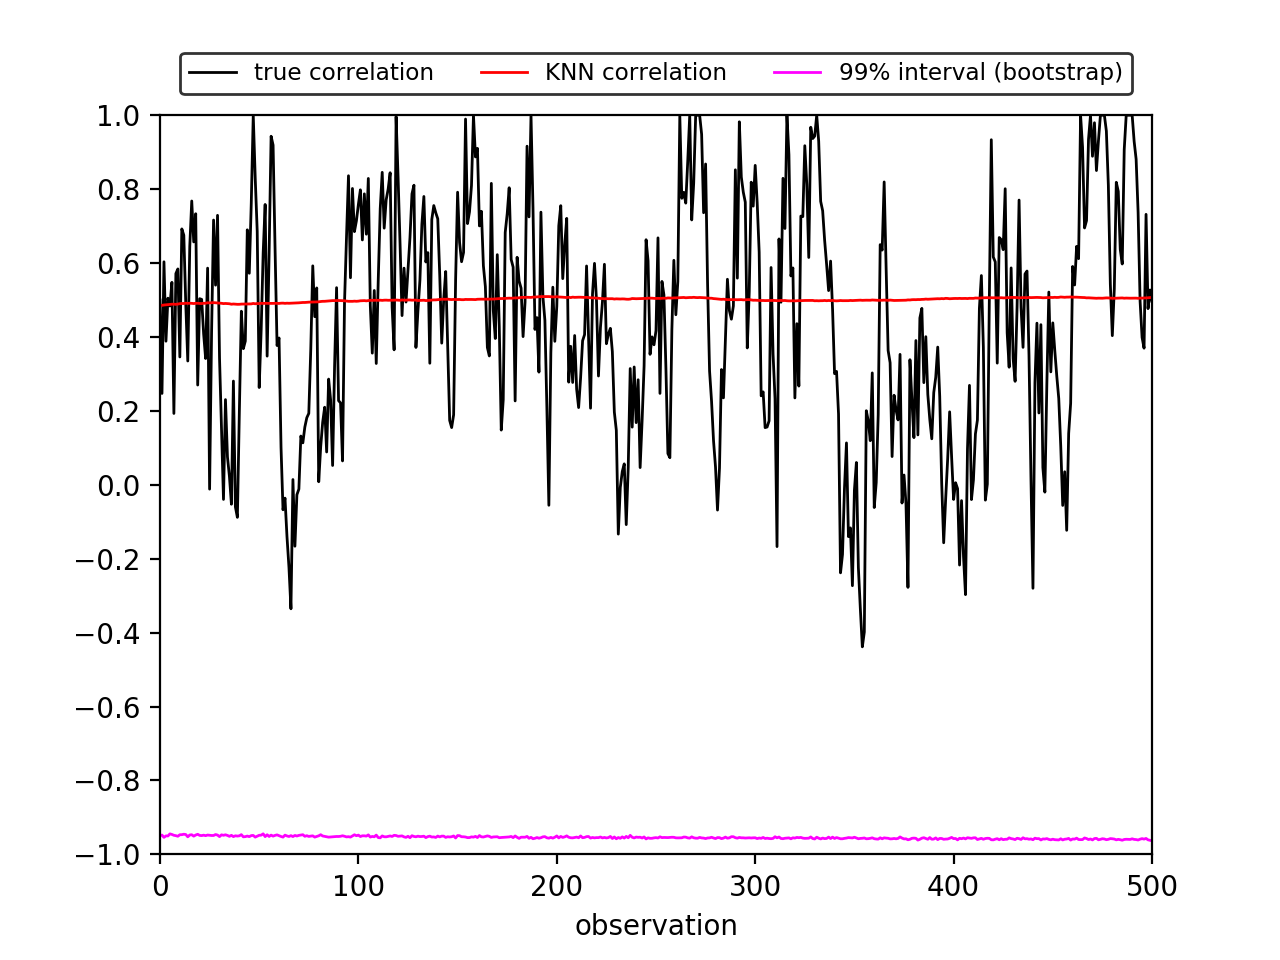
\includegraphics[width=\textwidth, height=0.5\textwidth]{knn_pearson_21_len_train_estimates_bootstrap_true.png} 
		\caption{KNN(unif) with $\Delta=21$ and Pearson covariates.} 	
		\label{fig:knn_pearson21_len_train_bootstrap_true}
	\end{subfigure}
	\hfill  
	\begin{subfigure}[b]{0.49 \textwidth}
		\centering 
		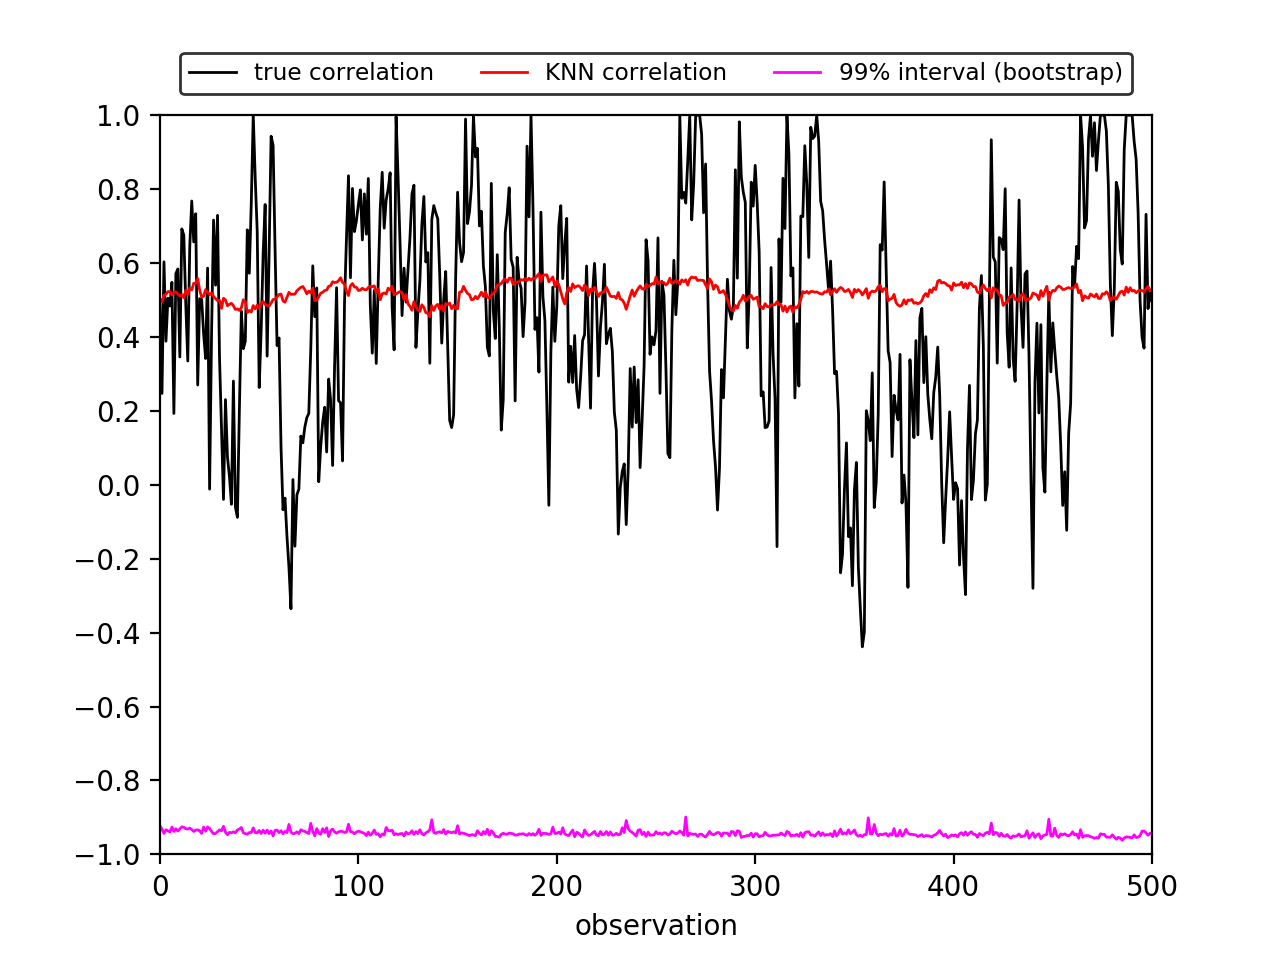
\includegraphics[width=\textwidth, height=0.5\textwidth]{knn_pearson_21_IDW_estimates_bootstrap_true.png} 
		\caption{KNN(idw) with $\Delta=21$ and Pearson covariates.} 
		\label{fig:knn_pearson21_IDW_bootstrap_true}
	\end{subfigure}
	\begin{subfigure}[b]{0.49 \textwidth}
		\centering 
		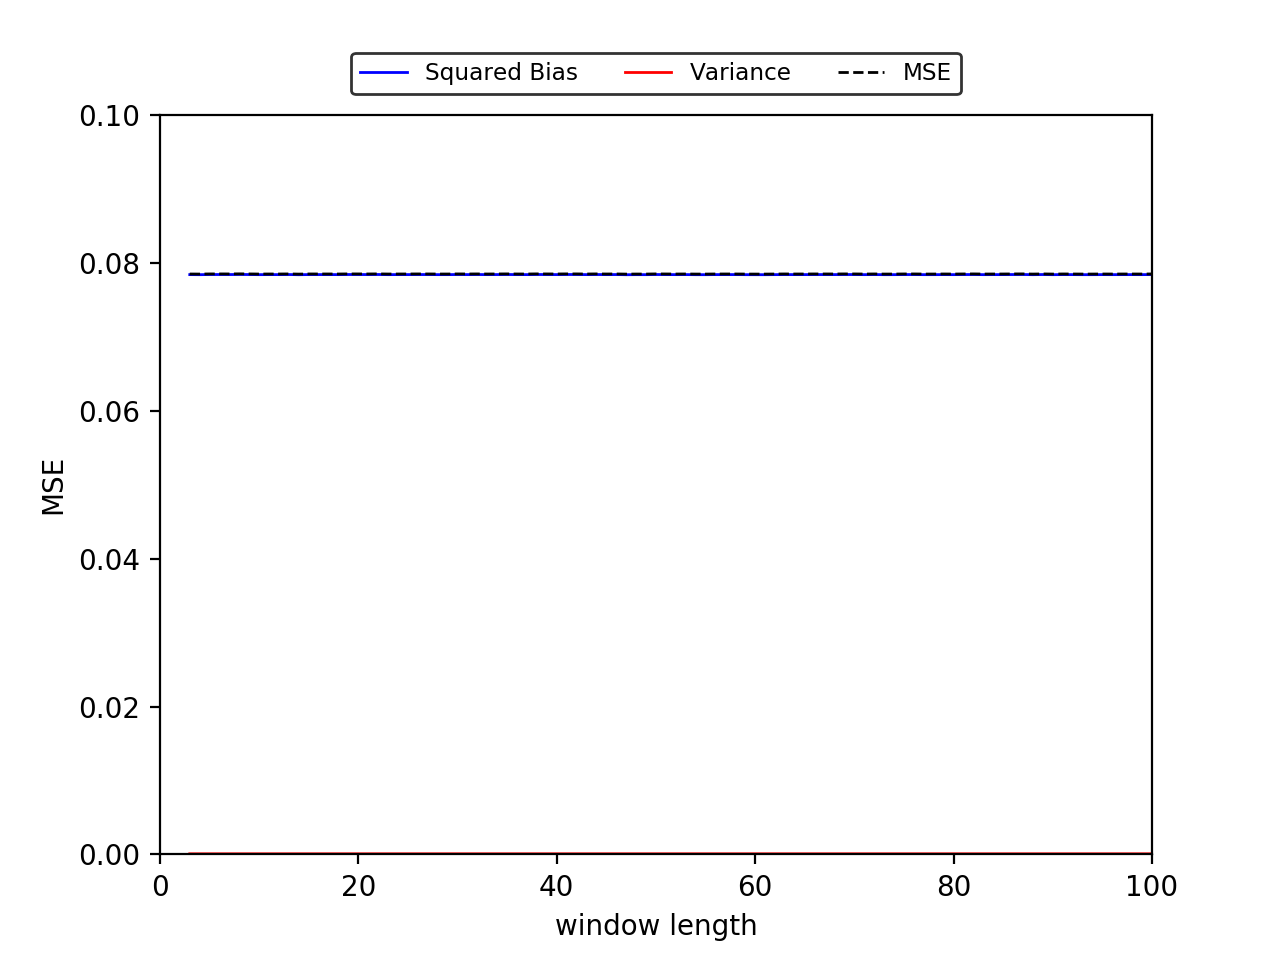
\includegraphics[width=\textwidth, height=0.5\textwidth]{decom_mse_knn_len_train_pearson_true.png} 
		\caption{Bias-variance decomposition for KNN(unif) estimates with Pearson as covariate.} 	
		\label{fig:decom_mse_knn_len_train_pearson_true}
	\end{subfigure}
	\hfill  
	\begin{subfigure}[b]{0.49 \textwidth}
		\centering 
		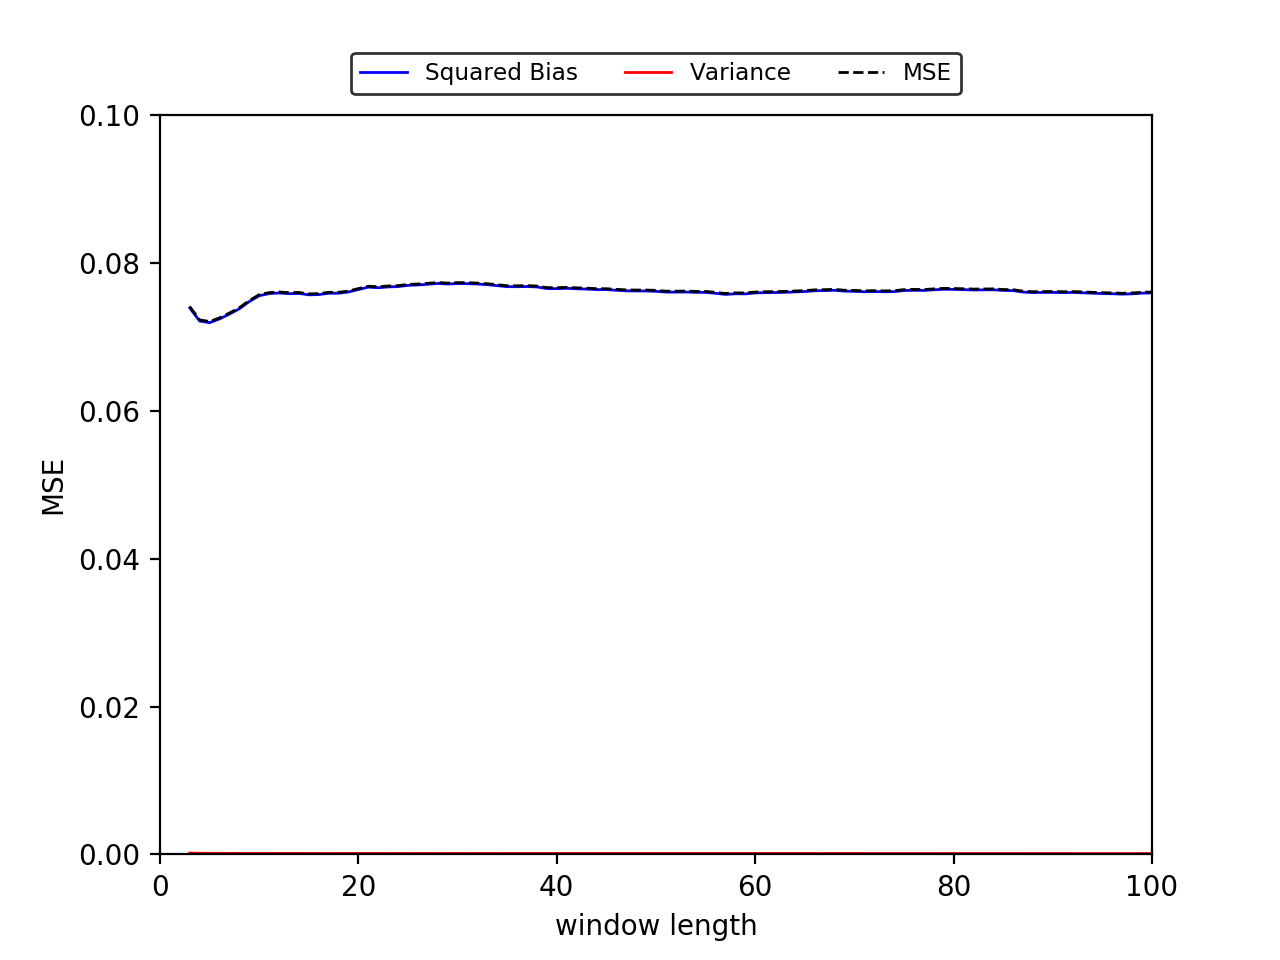
\includegraphics[width=\textwidth, height=0.5\textwidth]{decom_mse_knn_IDW_pearson_true.png} 
		\caption{Bias-variance decomposition for KNN(idw) estimates with Pearson as covariate.} 
		\label{fig:decom_mse_knn_IDW_pearson_true}
	\end{subfigure}
	\caption[MSE decomposition for KNN estimates with uniform and inverse distance weighting functions under true correlation.]{MSE for KNN estimates with uniform and inverse distance weighting functions, Pearson Moving Window bootstrap estimates as covariates and true correlation.}
	\label{fig:decom_mse_knn_len_train_IDW_pearson_kendall_true}
\end{figure}


\noindent
Furthermore, the alternative parameterizations of the KNN estimator with approximated covariates and response variable also satisfy the positive semidefiniteness condition of the conditional correlation matrix $R_t$ for the entire out-of-sample period under considered window lengths. Figure \ref{fig:det_knn_IDW_pearson_kendall_true.png} presents obtained minimum determinants of $R_t$ of KNN(idw) for all choices of window length\footnote{An uniform distance weighting function yields an approximately constant determinant of 0.74.}.  \\ 

\noindent
This section is concluded with a comparison of the function approximation capabilities of the KNN estimator and Pearson and Kendall sample correlation estimates using moving windows. Comparison is based on MSE between estimated and true correlations. Figure \ref{fig:mse_knn5_idw_pearson_kendall_true} presents MSE from KNN(5), an alternative parameterization with an inverse distance weighting function, KNN(idw), and Pearson and Kendall moving window estimates of conditional correlation. According to MSE, parameterizations of the KNN estimator where $k \in \{5, 10\}$ perform better than those of Pearson and Kendall moving window estimates for small window sizes but similarly for large window sizes. In contrast, parameterizations of the KNN estimator with an alternative distance weighting function and where the entire training data set is used for estimating correlation yields significantly smaller MSE compared to Pearson and Kendall sample correlation estimates using moving windows for all window sizes. In fact, the simulation study shows that the KNN estimator outperforms Pearson and Kendall sample correlation estimates for all window sizes when the number of neighbors $k \geq 25$ in addition to both alternative parameterizations. Finally, the variance of MSE from KNN(idw) estimates in figure \ref{fig:mse_knn5_idw_pearson_kendall_true} are 6.07e-6 and 8.55e-7, respectively, while that of Pearson and Kendall sample correlation estimates are 0.0040 and 0.0037, respectively. \\


\begin{figure}[H]  % [h] parameter makes sure figures are located at 'this' location.
	\centering
	\begin{subfigure}[b]{0.49 \textwidth}
		\centering 
		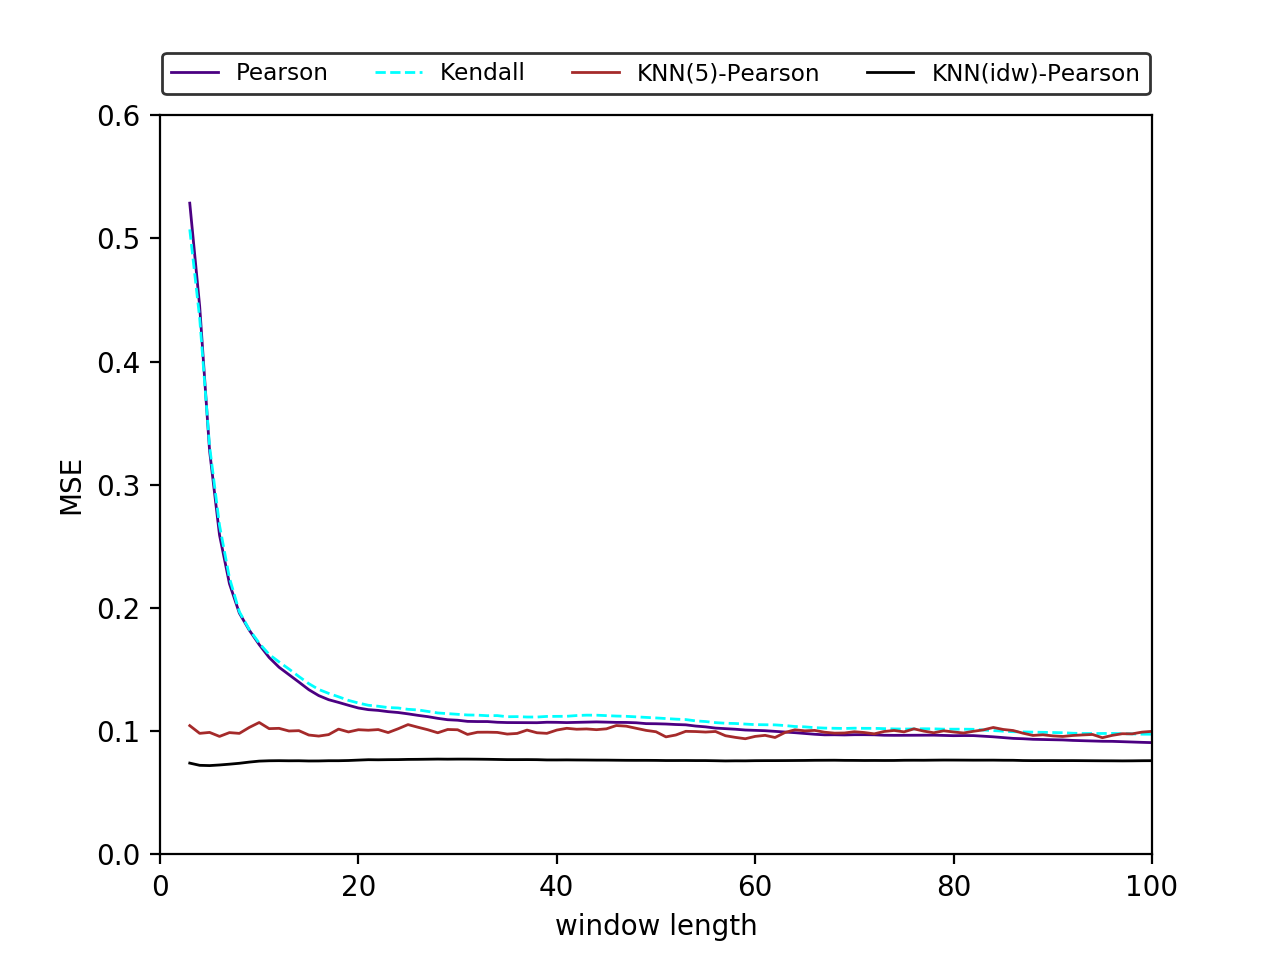
\includegraphics[width=\textwidth, height=0.5\textwidth]{mse_knn5_idw_pearson_kendall_true.png} 
		\caption{MSE for KNN with Pearson covariates and true correlation, Pearson and Kendall Moving Window bootstrap estimates.}
		\label{fig:mse_knn5_idw_pearson_kendall_true}
	\end{subfigure}
	\hfill
	\begin{subfigure}[b]{0.49 \textwidth}
		\centering 
		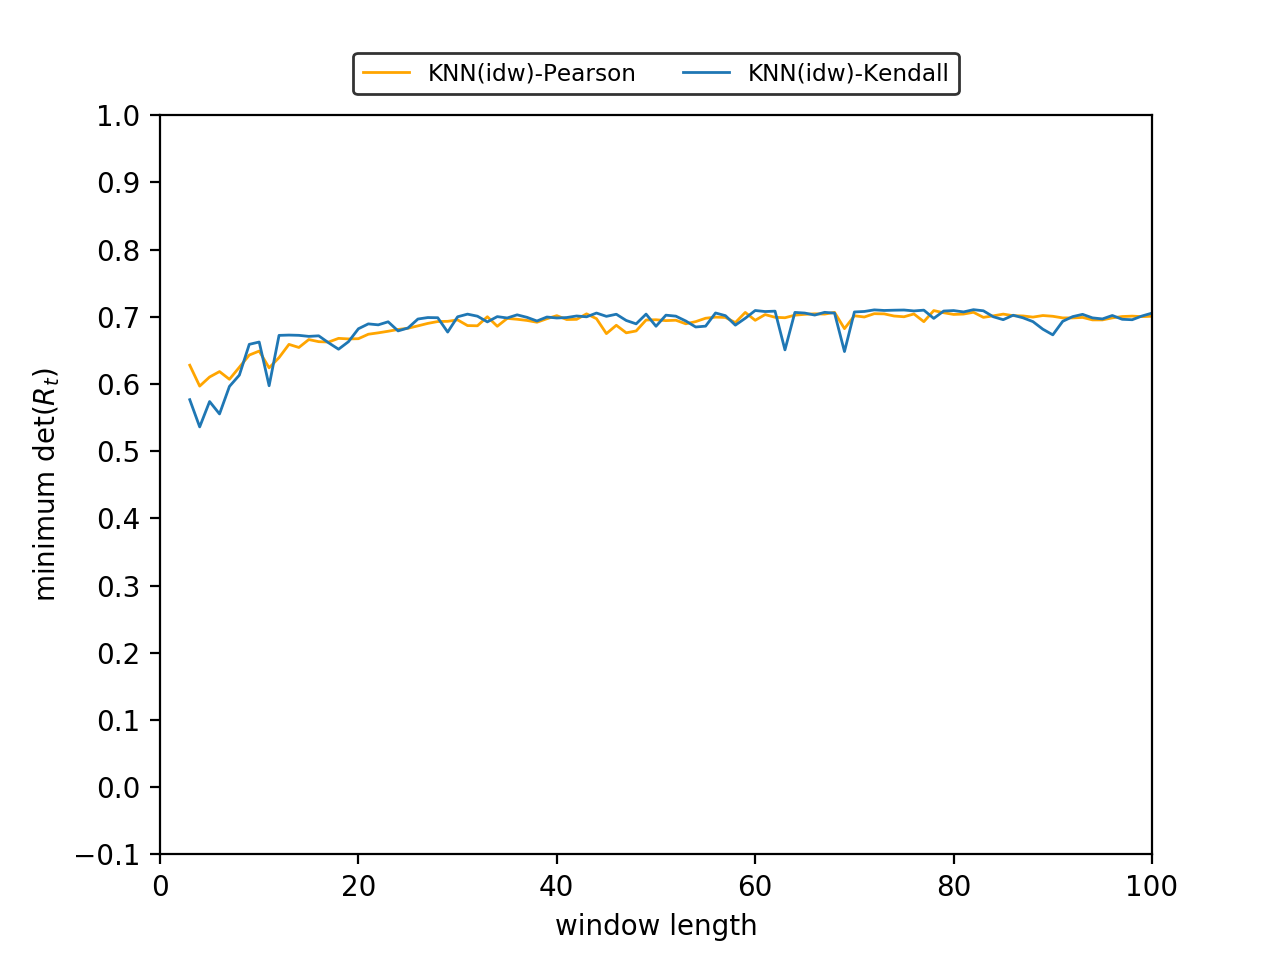
\includegraphics[width=\textwidth, height=0.5\textwidth]{det_knn_IDW_pearson_kendall_true.png} 
		\caption{Minimum determinants for KNN(idw) estimates with Pearson and Kendall covariates and true correlation.}
		\label{fig:det_knn_IDW_pearson_kendall_true.png}
	\end{subfigure}
	\caption[MSE and minimum determinants for KNN under true correlation, Pearson and Kendall Moving Window bootstrap estimates.]{Comparison MSE and minimum determinants for KNN with true correlation, Pearson and Kendall Moving Window bootstrap estimates.}
	\label{fig:mse_det_knn5_idw_pearson_kendall_true}
\end{figure}


%%%%%%% RANDOM FOREST TRUE COR %%%%%%%%%%%%%%
\subsection{Generalization Error of Random Forest under True Correlation} \label{sec:MSE_rf_true}
The accuracy of RF estimates with Pearson and Kendall covariates for conditional correlation is compared in terms of the MSE between estimated and true correlations. MSE from RF(10) with Pearson and Kendall moving window estimates of correlation for covariates are shown in figure \ref{fig:mse_rf10_pearson_kendall_true}. Regardless of the choice of window length, MSE from RF(10) with Pearson and Kendall covariates are between 0.0847 and 0.0980, and 0.0830 and 0.0983, respectively. The variance of MSE from RF(10) estimates with Pearson covariates is approximately 8.42e-6 while that of RF estimates with Kendall covariates is approximately 8.92e-6. Analogous to KNN estimates of correlation, RF thus appears to be rather insensitive to the choice of window length, regardless whether the set of covariates is constructed from Pearson or Kendall moving window estimates of correlation. 

\begin{figure}[H]
	\centering
	\begin{subfigure}[b]{0.49 \textwidth} 
		\centering
		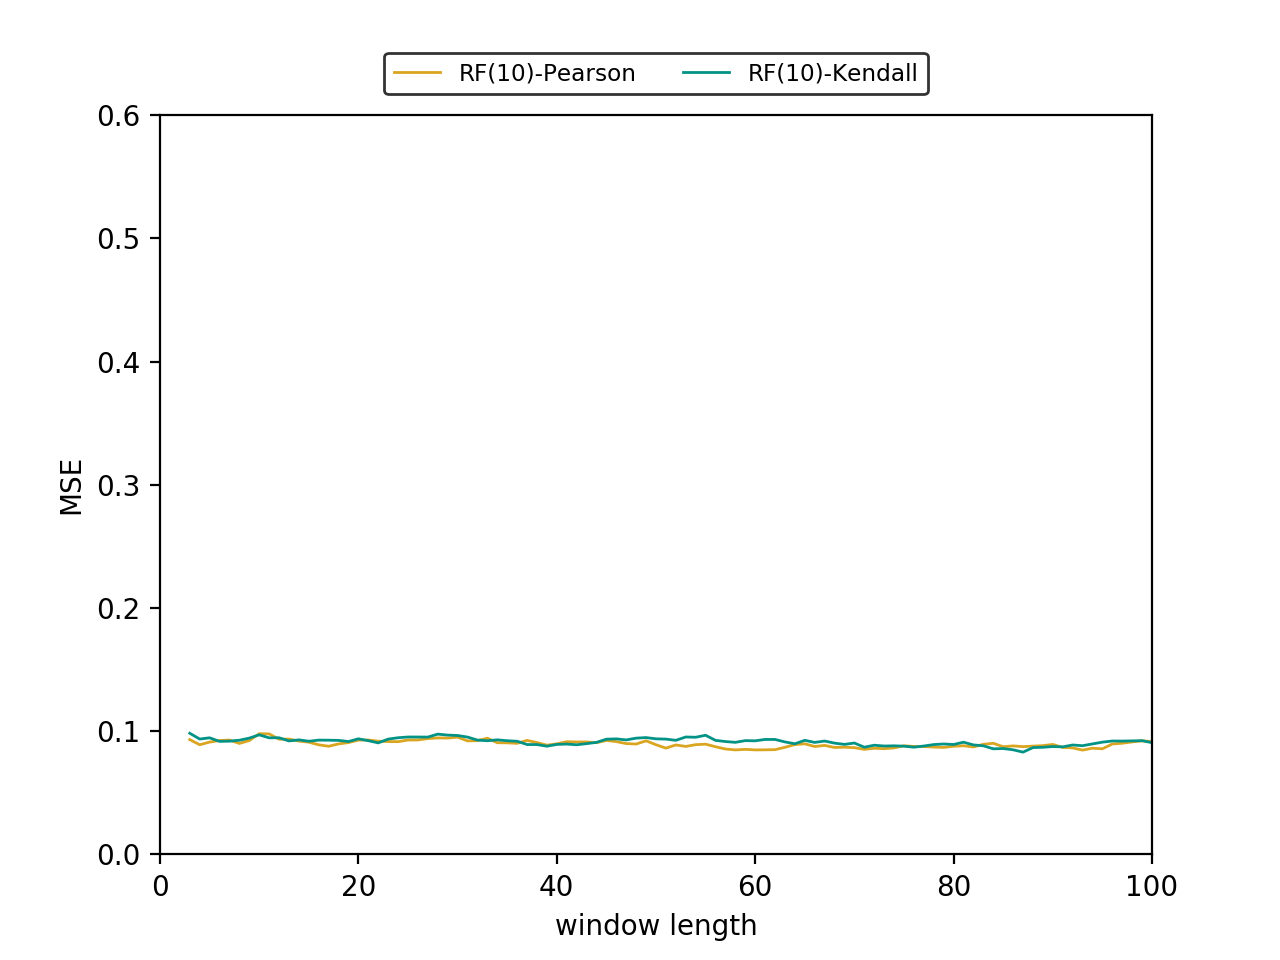
\includegraphics[width=\textwidth, height=0.5\textwidth]{mse_rf10_pearson_kendall_true}
		\caption{MSE for RF(10) with covariates from Pearson and Kendall and true correlation.}
		\label{fig:mse_rf10_pearson_kendall_true}
	\end{subfigure}
	\hfill
	\begin{subfigure}[b]{0.49 \textwidth} 
		\centering
		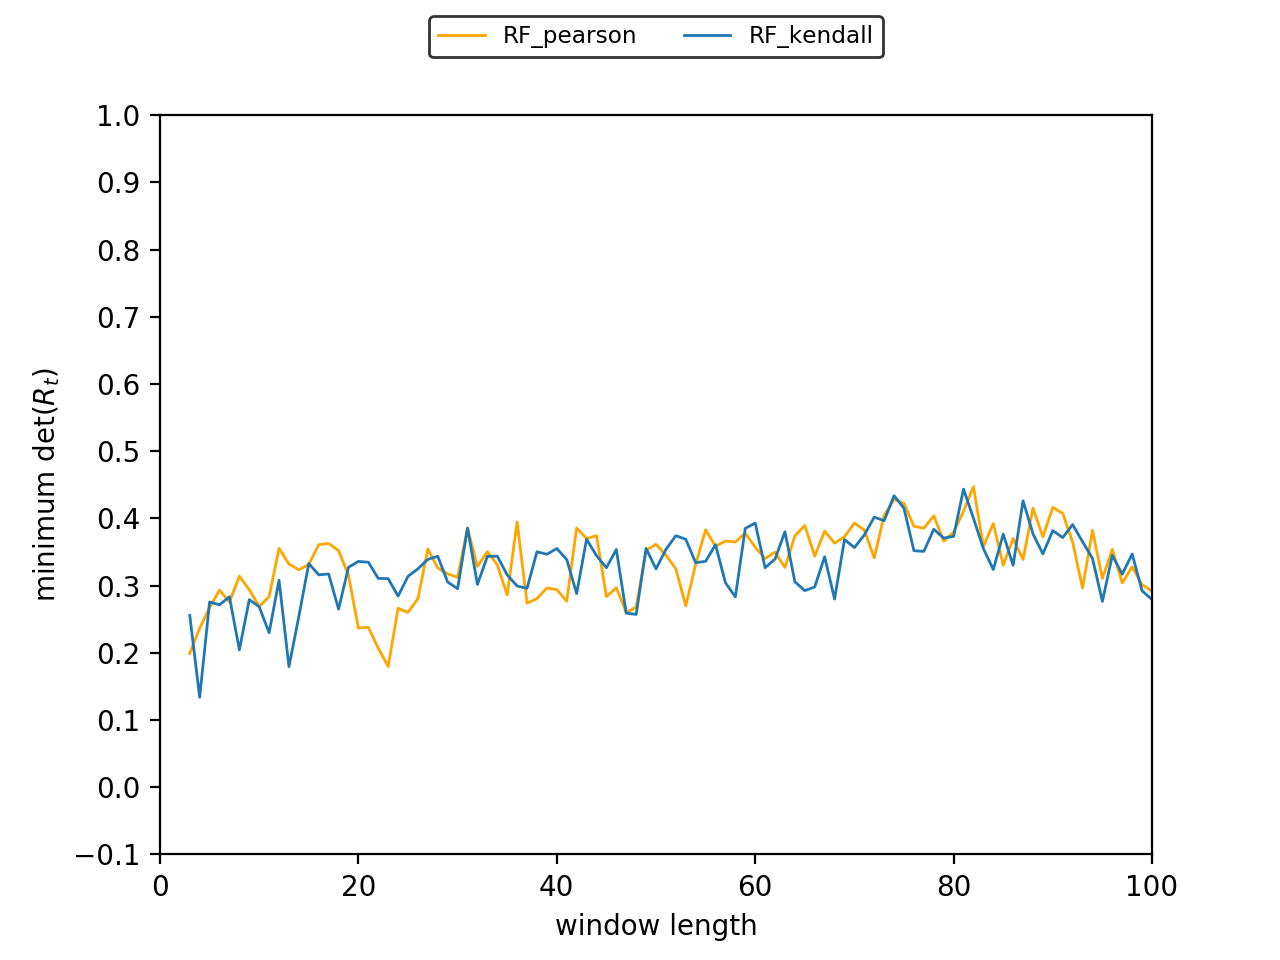
\includegraphics[width=\textwidth, height=0.5\textwidth]{det_rf10_pearson_kendall_true}
		\caption{Minimum determinants for RF(10) with covariates from Pearson and Kendall and true correlation.}
		\label{fig:det_rf10_pearson_kendall_true}
	\end{subfigure}
	\caption[MSE and minimum determinants for RF(n\_trees=10) under true correlation.]{Comparison MSE and minimum determinants for RF(n\_trees=10) with covariates from Pearson and Kendall and true correlation.}
	\label{fig:mse_det_rf10_pearson_kendall_true}
\end{figure}

\clearpage 
\noindent
Figure \ref{fig:det_rf10_pearson_kendall_true} presents obtained minimum determinants of $R_t$ for all choices of window length; RF(10) estimates of conditional correlation satisfy the positive semidefiniteness condition in the conditional correlation matrix $R_t$ for the entire out-of-sample period under all considered choices of window length.  \\


\noindent
From visual inspection of the plots in figures \ref{fig:rf_pearson21_bootstrap_true}-\ref{fig:rf_kendall21_bootstrap_true} it seems that the uncertainty in the conditional correlation $\rho_t$, which is illustrated by the 99\% confidence interval, seems smaller for RF(10) estimates compared to Pearson and Kendall moving window estimates under the same window length of 21. Analogous to KNN(5) estimates of correlation, the RF estimator with a small number of decision trees, such as RF(10), produces correlation estimates that  are much more volatile than Pearson and Kendall sample correlations using moving windows. This may be a less desirable result as it is not expected that correlation between assets changes that drastically at each time unit. Rather, correlation is expected to vary gradually over time \citep{ref:Basturk2016} \\


\begin{figure}[H]  % [h] parameter makes sure figures are located at 'this' location.
	\centering
	\begin{subfigure}[b]{0.49 \textwidth} % sum of widths should be less than text width if all one the same line
		\centering 
		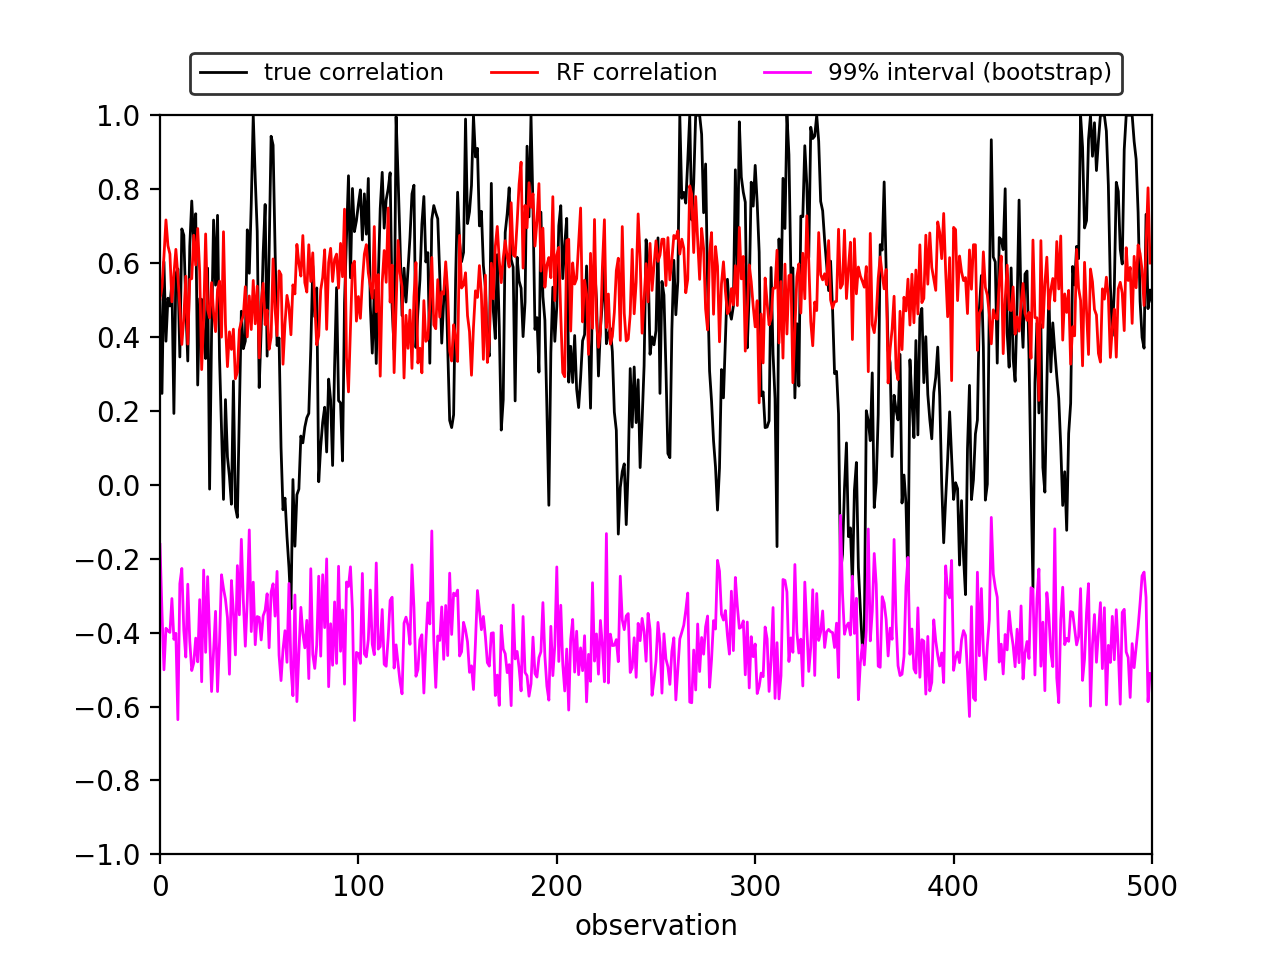
\includegraphics[width=\textwidth, height=0.5\textwidth]{rf_pearson_21_estimates_bootstrap_true.png} 
		\caption{RF(10) estimates with $\Delta=21$, Pearson as covariate and true correlation.} 	
		\label{fig:rf_pearson21_bootstrap_true}
	\end{subfigure} 
	\hfill	
	\begin{subfigure}[b]{0.49 \textwidth} 
		\centering 
		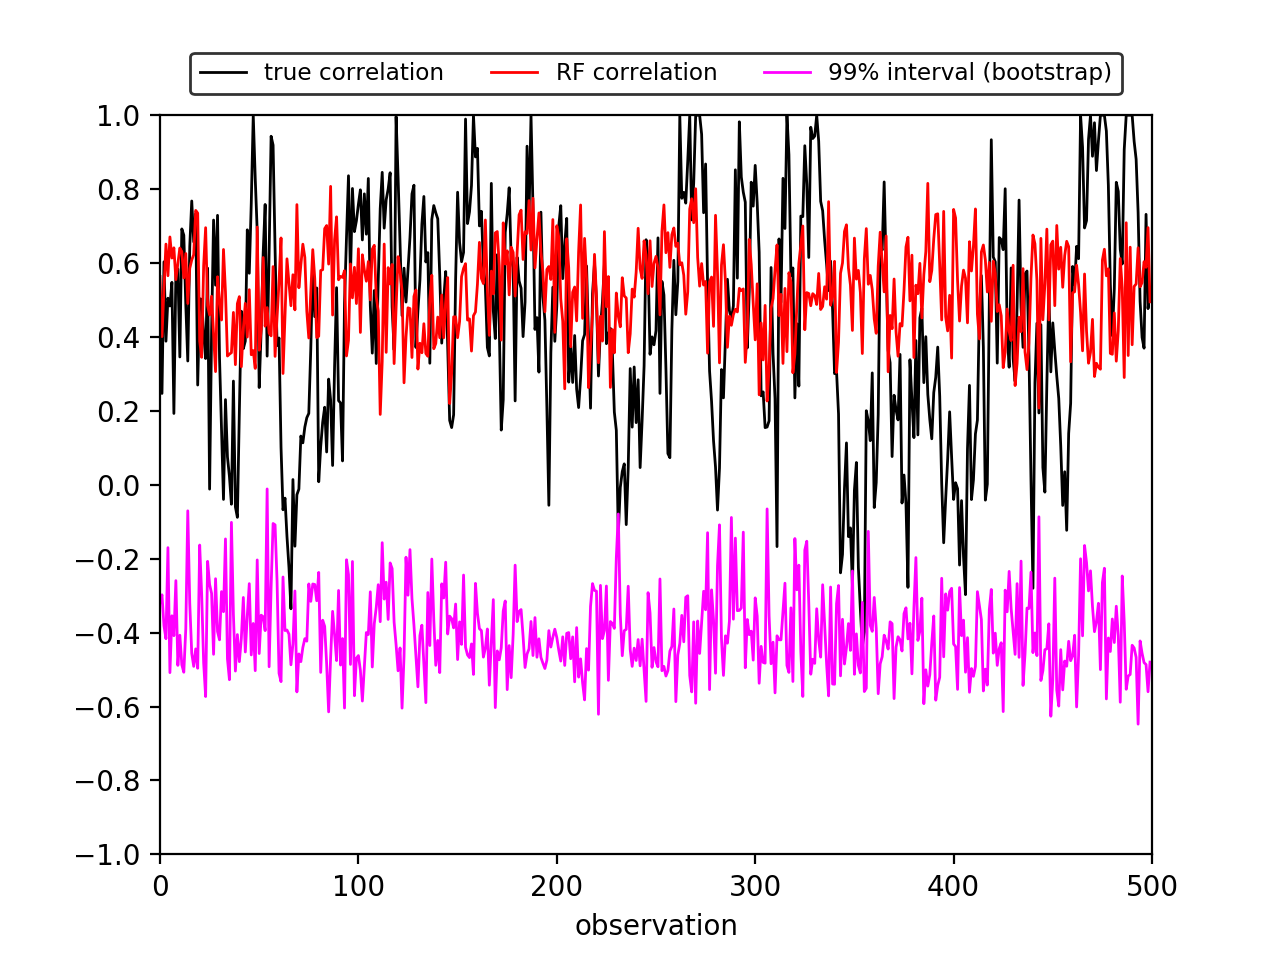
\includegraphics[width=\textwidth, height=0.5\textwidth]{rf_kendall_21_estimates_bootstrap_true.png} 
		\caption{RF(10) estimates with $\Delta=21$, Kendall as covariate and true correlation.} 
		\label{fig:rf_kendall21_bootstrap_true}
	\end{subfigure} 
	\hfill	
	\begin{subfigure}[b]{0.49 \textwidth}
		\centering 		
		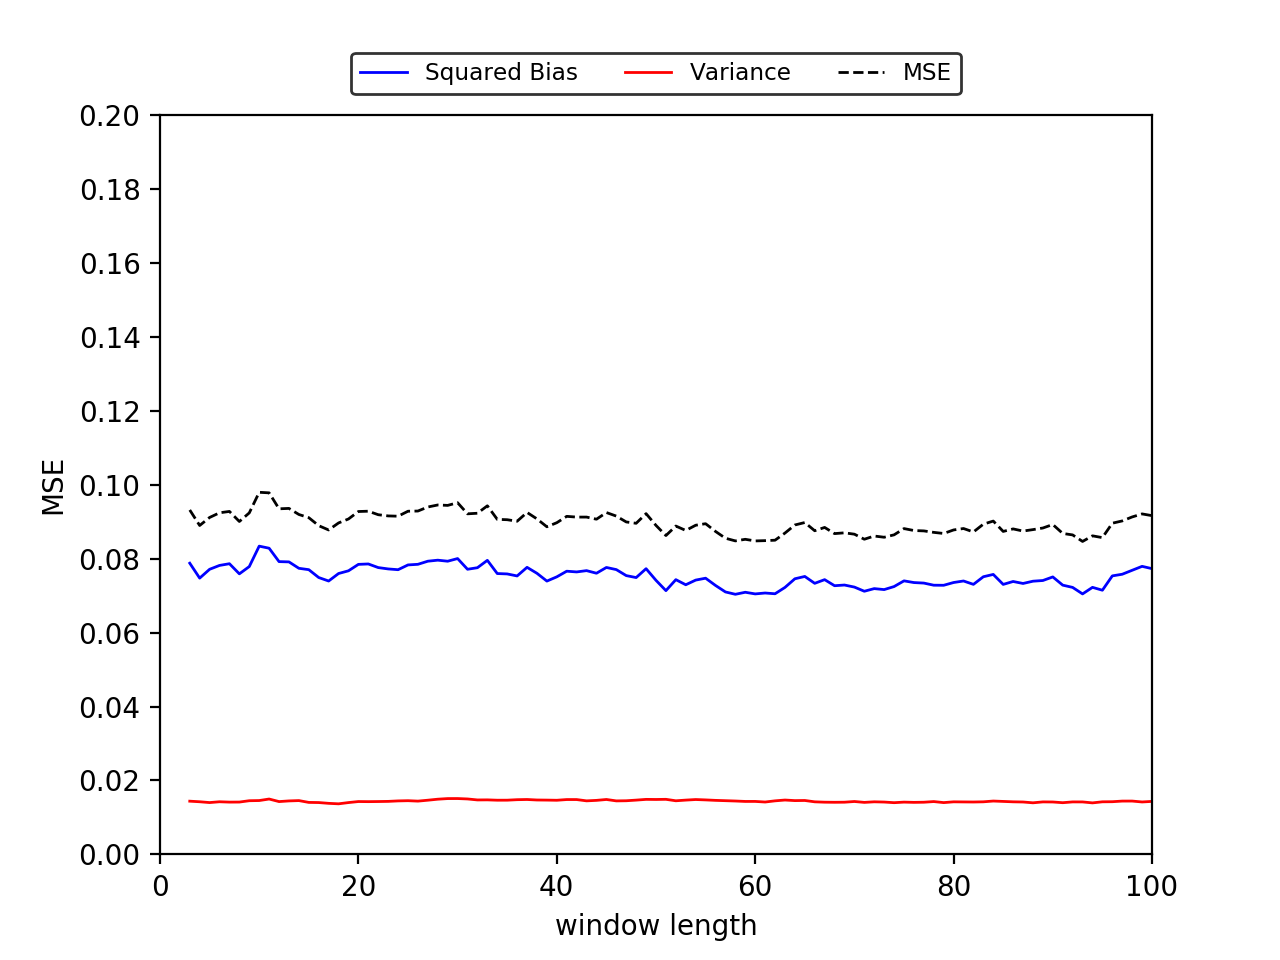
\includegraphics[width=\textwidth, height=0.5\textwidth]{decom_mse_rf10_pearson_true.png} 
		\caption{Bias-variance decomposition for RF(10) estimates with Pearson as covariate and true correlation.} 
		\label{fig:decom_mse_rf10_pearson_true}
	\end{subfigure}
	\hfill  
	\begin{subfigure}[b]{0.49 \textwidth}
		\centering 
		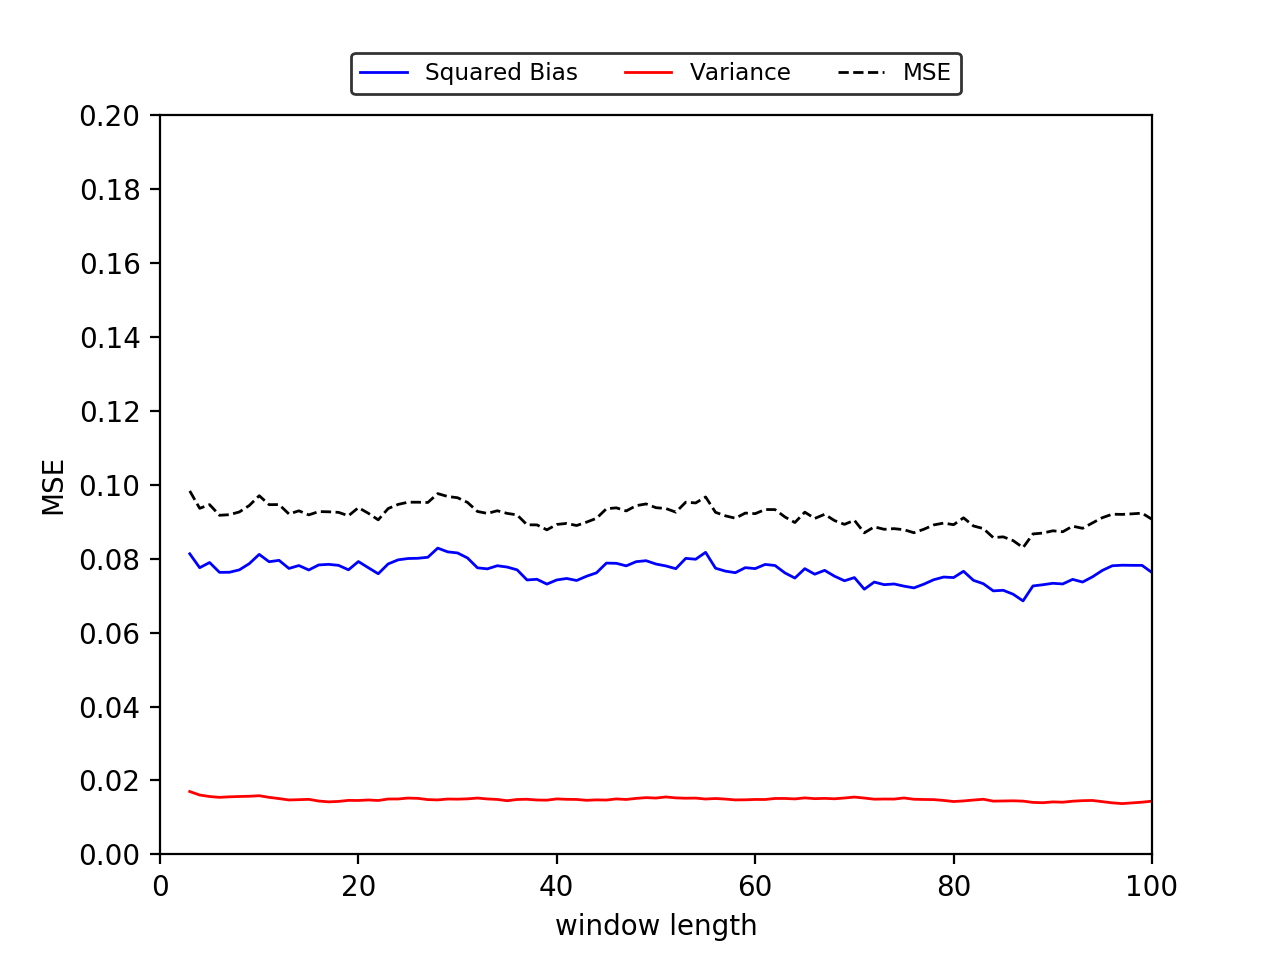
\includegraphics[width=\textwidth, height=0.5\textwidth]{decom_mse_rf10_kendall_true.png} 
		\caption{Bias-variance decomposition for RF(10) estimates with Kendall as covariate and true correlation.} 
		\label{fig:decom_mse_rf10_kendall_true}
	\end{subfigure}
	\caption[MSE decomposition for RF(10) under true correlation.]{MSE for RF(10) estimates with Pearson and Kendall Moving Window bootstrap estimates as covariates and true correlation.}
	\label{fig:decom_mse_rf10_pearson_kendall_true}
\end{figure}

\noindent
The MSE decomposition into bias and variance terms from RF(10) estimates of correlation are shown in figures \ref{fig:decom_mse_rf10_pearson_true}-\ref{fig:decom_mse_rf10_kendall_true}. These figures indicate that the RF(10) estimator is considerably less sensitive to the choice of the window length for smaller window sizes when compared to Pearson and Kendall sample correlations using moving windows depicted in figure \ref{fig:mse_pearson_kendall_bootstrap}. In fact, the uncertainty around the estimated correlations appears to be marginally affected by the choice of the window length for all window sizes, which is corroborated by the fact that the variance as a function of the window length behaves like a (more or less) constant red line in these figures (analogue to KNN).

\subsection{Effect of Alternative Random Forest Parameterizations under True Correlation} \label{sec:MSE_rf_alt_true}
Simulation results in presented in tabel \ref{tab:mse_decomp_rf_pearson_kendall_true}\footnote{Results were obtained by taking 100 bootstrapped samples instead of 1000 due to computational time constraints. This number of bootstrapped samples is however sufficient for illustrational purposes.} show an inverse relationship between the number of decision trees in the random forest and the uncertainty around the estimated correlations, regardless whether Pearson or Kendall estimates are used for specification of the set of covariates. It is clearly observed that an increase in the number of decision trees results in a decrease of the variance, and conversely. This observation is in line with our discussion on MSE decomposition for the RF estimator in section \ref{sec:mse_decompose}. For the correlation dynamics generated by \eqref{eq:correlation_simulation}, it is observed that the point of diminishing reduction in variance is reached around 300 decision trees. An increase in number of decision trees after that does not significantly reduce the variance. \\  

\noindent
With respect to our discussion on the effect of random covariate selection in individual tree construction on the squared bias and variance (section \ref{sec:mse_decompose}): the individual decision trees of the random forest in our simulation study are merely decision stumps as the dimension of the covariate set is only three (minimum and maximum returns and pairwise correlation of the previous time unit), that is, $P=3$, which means that under default randomization for regression problems $p=P/3 = 1$. As such, no sensitivity analysis is undertaken on the number of covariates given the small dimension of the covariate set. This may, however, be interesting in high dimensional systems of correlations. \\  


%% TABLE
\begin{table}[H]
\centering
\captionsetup[subtable]{position=below}
%\captionsetup[table]{position=below}
\begin{subtable}{0.49\linewidth}
\centering
\begin{tabular}{r  c  c  c} 
\toprule
\multicolumn{1}{ r }{\textbf{Trees}} &
\multicolumn{1}{ c }{\textbf{Squared Bias}} &
\multicolumn{1}{ c }{\textbf{Variance}} &
\multicolumn{1}{ c }{\textbf{MSE}} \\
\midrule 

10                                   &   0.0839                       & 0.0144                & 0.0983      \\
100                                 & 0.0839                         & 0.0077               & 0.0916       \\
300                                 & 0.0837                         & 0.0071               & 0.0908      \\
600                                 & 0.0841                         & 0.0070               & 0.0911     \\
1000                               & 0.0837                         &  0.0069              & 0.0906     \\ [1ex]

\bottomrule
\end{tabular}
\caption{MSE for RF estimates with $\Delta=10$, Pearson as covariate and true correlation.}
\label{tab:mse_decomp_rf_pearson_true}
\end{subtable}
\hfill
\begin{subtable}{0.49\linewidth}
\centering
\begin{tabular}{r  c  c  c} 
\toprule
\multicolumn{1}{ r }{\textbf{Trees}} &
\multicolumn{1}{ c }{\textbf{Squared Bias}} &
\multicolumn{1}{ c }{\textbf{Variance}} &
\multicolumn{1}{ c }{\textbf{MSE}} \\
\midrule 

10                                   & 0.0817                         & 0.0158               &  0.0976     \\
100                                 & 0.0815                         & 0.0088               & 0.0903      \\
300                                 & 0.0813                         & 0.0082               & 0.0895      \\
600                                 & 0.0817                         & 0.0082               & 0.090     \\
1000                               &  0.0814                         &  0.0080             & 0.0894     \\ [1ex]

\bottomrule
\end{tabular}
\caption{MSE for RF estimates with $\Delta=10$, Kendall as covariate and true correlation.}
\label{tab:mse_decomp_rf_kendall_true}
\end{subtable}
\caption{MSE decomposition as a function of the number trees for RF estimator with proxy covariates and true correlation.}
\label{tab:mse_decomp_rf_pearson_kendall_true}
\end{table}

\noindent
This section is concluded with a comparison of the function approximation capabilities of the RF estimator and Pearson and Kendall sample correlation estimates using moving windows. Comparison is based on MSE between estimated and true correlation. Figure \ref{fig:mse_rf10_pearson_kendall_comp_true.png} presents MSE from RF(10) and Pearson and Kendall moving window estimates of conditional correlation. According to MSE, RF(10) estimator shows significantly smaller MSE compared to Pearson and Kendall sample correlation estimates for all window sizes. Finally, the variance of MSE from RF(10) estimates with Pearson and Kendall covariates and true correlation are 8.42e-6 and 8.92e-6, respectively, while that of Pearson and Kendall moving window estimates are 0.0040 and 0.0037, respectively. \\


\begin{figure}[H]
	\centering
	\begin{subfigure}[b]{0.49 \textwidth} 
		\centering
		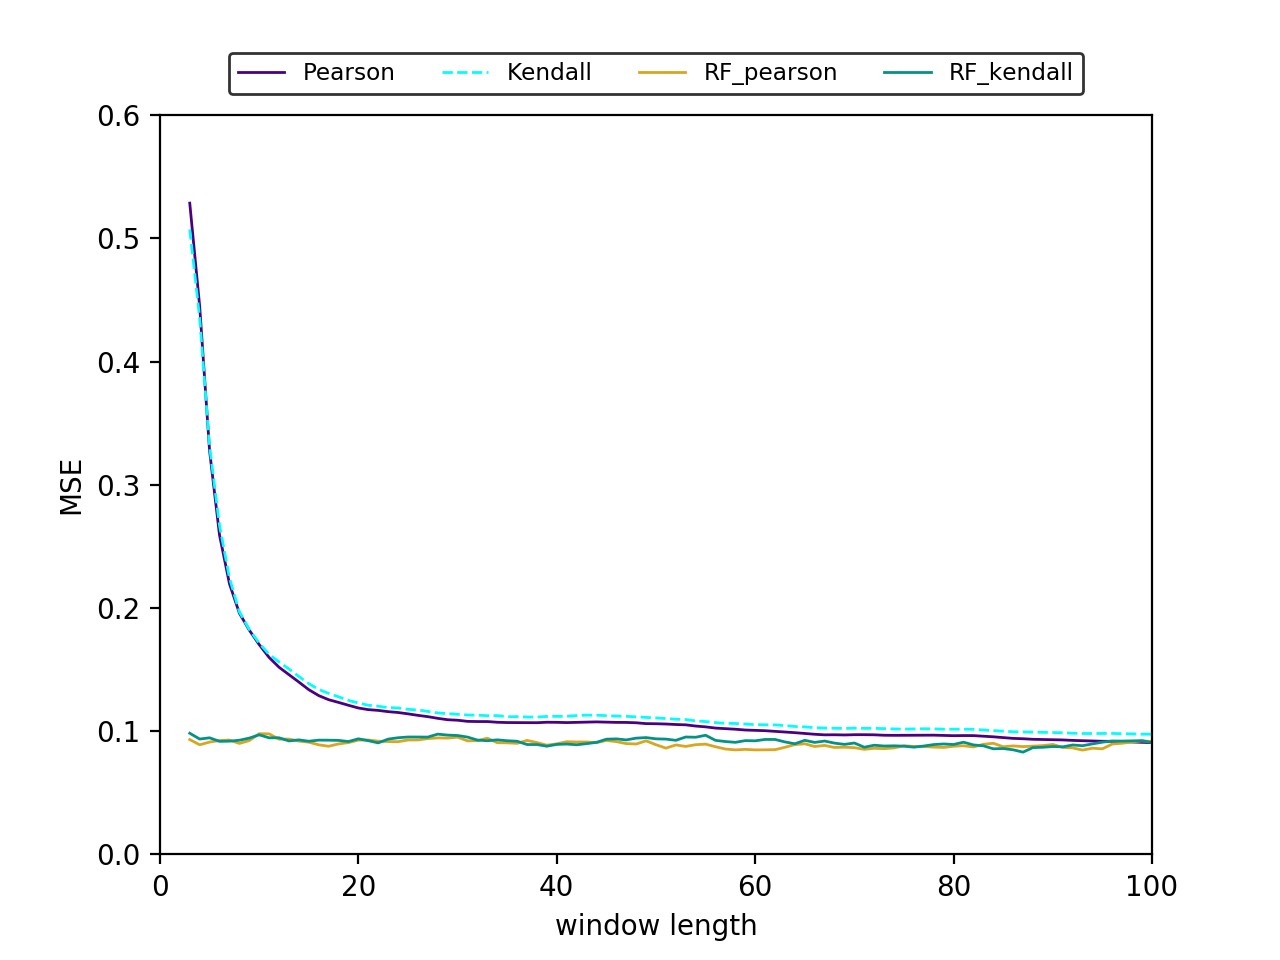
\includegraphics[width=\textwidth, height=0.5\textwidth]{mse_rf10_pearson_kendall_comp_true.png}
		%\caption{MSE for RF with covariates from Pearson and Kendall and true correlation.}
		%\label{fig:mse_rf10_pearson_kendall_comp_true.png}
	\end{subfigure}
	\caption[MSE for RF(10) under true correlation, Pearson and Kendall Moving Window bootstrap estimates.]{Comparison MSE for RF(10) with true correlation, Pearson and Kendall Moving Window bootstrap estimates.}
	\label{fig:mse_rf10_pearson_kendall_comp_true.png}
\end{figure}

%%%%%%%%%%%%%%%%%%%%%%%%%%%%%%%%%%%%%
%%%%%%%%%% Proxies for Correlation %%%%%%%%%%%%%%%%
%%%%%%%%%%%%%%%%%%%%%%%%%%%%%%%%%%%%%%
\section{Learning with Proxy for Response Variable} \label{sec:proxy_correlation}
This section is premised on a more realistic approach to verify the adequacy of k-nearest neighbor and random forest as estimators of conditional correlation. Both the covariates and response variable are obtained from Pearson or Kendall sample estimates using moving windows, as defined in \eqref{eq:mw_rho} and \eqref{eq:mw_kendall}, respectively. This is different from section \ref{sec:true_correlation} where the response variable of the learning estimators was defined as the true observed correlation (given by the simulated parameters). This setup in this section allows us to study the effect of using approximations of true correlations for both covariates and response variable on a statistical loss function, that is, the mean squared error. \\

%%%%%% NEAREST NEIGHBOR PROXY 	%%%%%%%%
\subsection{Generalization Error of Nearest Neighbor under Proxy Correlation} \label{sec:MSE_knn_proxy}
The accuracy of KNN estimates with Pearson and Kendall sample correlation estimates using moving windows for both covariates and response variable is compared in terms of the mean squared error (MSE) between estimated and true correlation. MSE from KNN(5) with Pearson and Kendall moving window estimates of correlation is shown in figure \ref{fig:mse_knn5_pearson_kendall_proxy}. Regardless of the choice of window length, MSE from KNN(5) with Pearson and Kendall covariates are between 0.0855 and 0.2555, and 0.0952 and 0.2223, respectively. The variance of MSE from KNN(5) estimates with Pearson covariates is approximately 5.70e-4 while that of KNN(5) estimates with Kendall covariates is approximately 2.96e-4. Recall that in figure \ref{fig:mse_knn5_pearson_kendall_true} the KNN(5) estimator appeared to be insensitive to the choice of window length when the response variable is specified by the true correlation. Interestingly, figure \ref{fig:mse_knn5_pearson_kendall_proxy} shows that MSE from KNN(5) estimation with Pearson or Kendall approximations for the response variable varies substantially for smaller window sizes. Although, less variation is observed when compared with MSE from Pearson and Kendall moving window estimates depicted in figure \ref{fig:mse_pearson_kendall_bootstrap}. Furthermore, KNN(5) estimates of conditional correlation with both the set of covariates and response variable approximations of true correlation satisfy the positive semidefiniteness condition in the conditional correlation matrix $R_t$ for the entire out-of-sample period under all choices of window length. Figure \ref{fig:det_knn5_pearson_kendall_proxy} presents the obtained minimum determinants of $R_t$ for all choices of window length.  
     
\begin{figure}[H]
	\centering
	\begin{subfigure}[b]{0.49 \textwidth} 
		\centering
		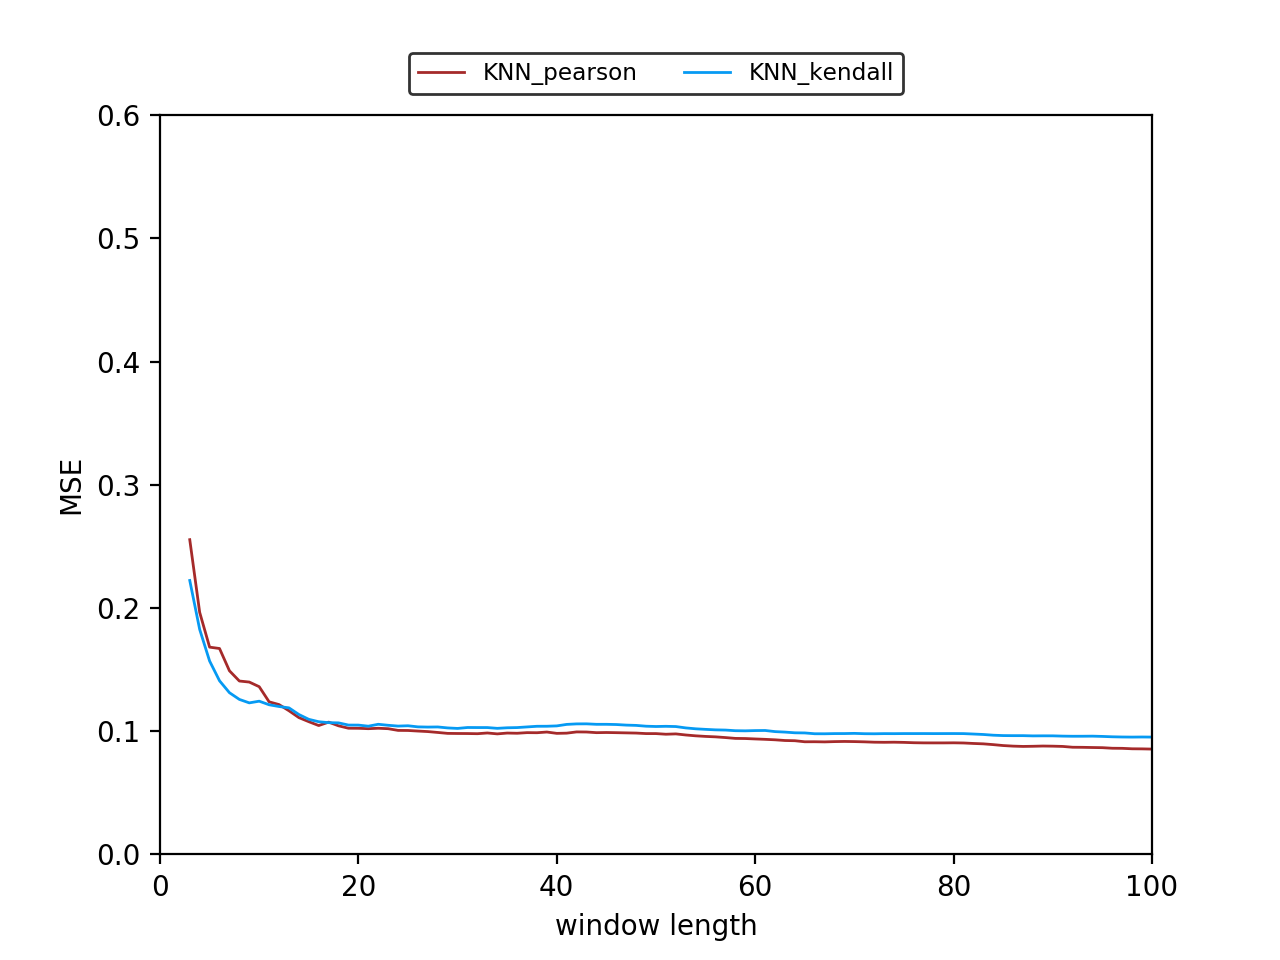
\includegraphics[width=\textwidth, height=0.5\textwidth]{mse_knn5_pearson_kendall_proxy.png}
		\caption{MSE for KNN(5) with covariates from Pearson and Kendall and proxy correlation.}
		\label{fig:mse_knn5_pearson_kendall_proxy}
	\end{subfigure}
	\hfill
	\begin{subfigure}[b]{0.49 \textwidth} 
		\centering
		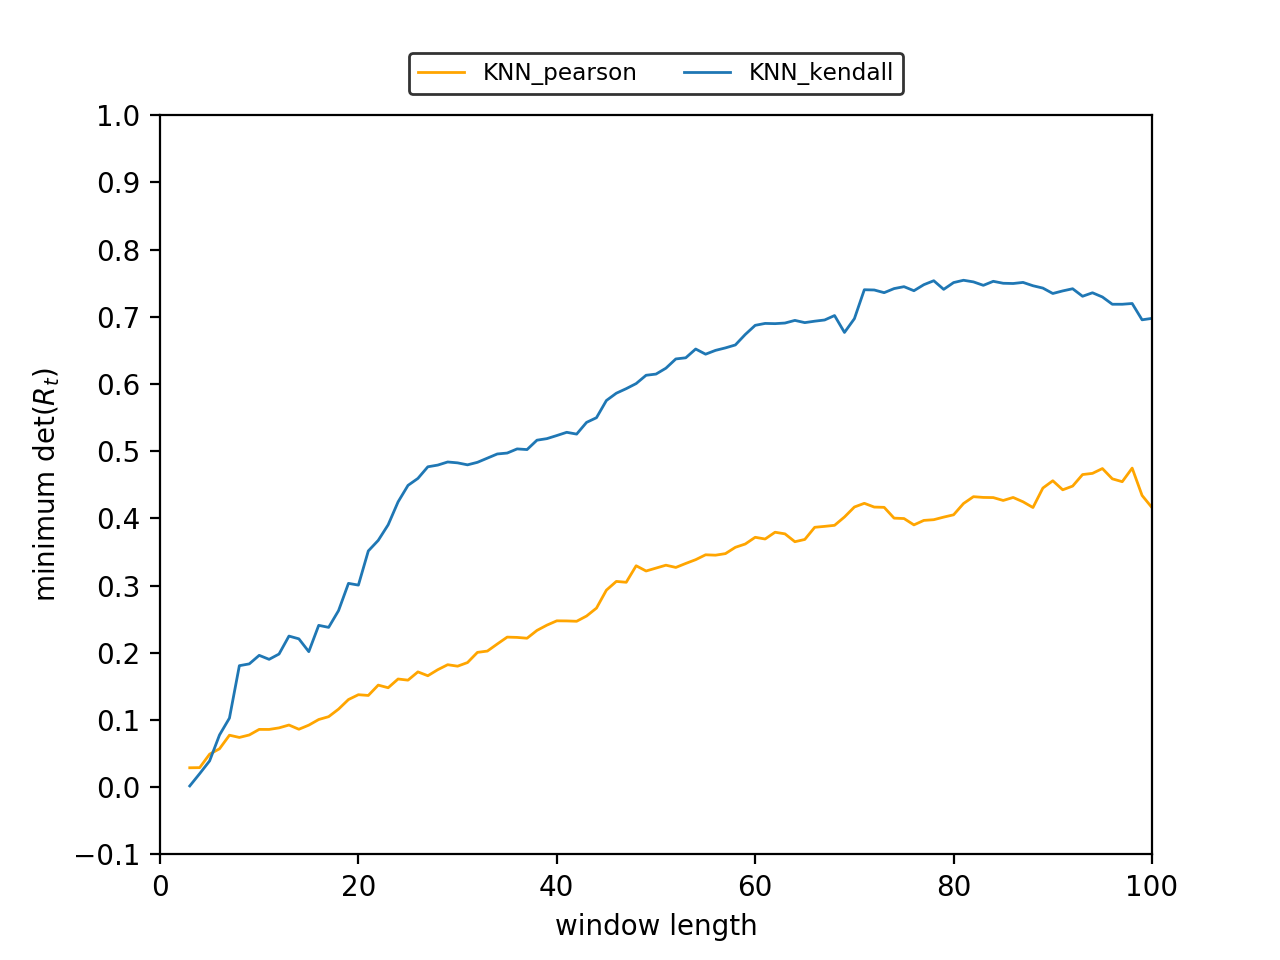
\includegraphics[width=\textwidth, height=0.5\textwidth]{det_knn5_pearson_kendall_proxy.png}
		\caption{Minimum determinants for KNN(5) with covariates from Pearson and Kendall and proxy correlation.}
		\label{fig:det_knn5_pearson_kendall_proxy}
	\end{subfigure}	
	\caption[MSE and minimum determinants for KNN(n\_neighbors=5) under proxy correlation.]{Comparison MSE and minimum determinants for KNN(n\_neighbors=5) with covariates from Pearson and Kendall and proxy correlation.}
	\label{fig:mse_det_knn5_pearson_kendall_proxy}
\end{figure}

\noindent
From visual inspection of the plots in figures \ref{fig:knn_pearson21_bootstrap_proxy}-\ref{fig:knn_kendall21_bootstrap_proxy} it is clear that the uncertainty in the conditional correlation $\rho_t$, 
which is illustrated by the $99\%$ confidence interval, is smaller for KNN(5) estimates compared to Pearson and Kendall moving window estimates, even though both the set of covariates and the response variable of the KNN estimator are now based on approximations of correlation instead of true correlation. These figures also show smaller uncertainty in the conditional correlation $\rho_t$ when compared with KNN(5) estimates with true correlation as the response variable, which are depicted in figure \ref{fig:decom_mse_knn5_pearson_kendall_proxy}. Moreover, KNN estimates of correlation with true correlation as response variable in figures \ref{fig:knn_pearson21_bootstrap_true}\ref{fig:knn_kendall21_bootstrap_true} are much more volatile. In contrast, KNN estimates with approximated response variable in figures \ref{fig:knn_pearson21_bootstrap_proxy}-\ref{fig:knn_kendall21_bootstrap_proxy} follow the increases and decreases of the true correlation smoother, with tighter confidence intervals. \\ 

\noindent
The MSE decomposition into bias and variance terms from KNN(5) estimates of correlation are shown in figures \ref{fig:decom_mse_knn_pearson_proxy}-\ref{fig:decom_mse_knn_kendall_proxy}. These figures indicate that the KNN(5) estimator with approximated response variable is more sensitive to the choice of the window length for smaller window sizes compared with the KNN(5) estimator with true correlation depicted in figure \ref{fig:decom_mse_knn5_pearson_kendall_true}. This observation can be explained by error propagation: the effect of covariates' uncertainties (or errors) on the error of the function based on them. In the case when a KNN estimator uses approximated response variables for learning, the error associated with approximation of true correlation using moving window estimates is propagated to the response of the KNN estimator. Interestingly, figures \ref{fig:decom_mse_knn_pearson_proxy}-\ref{fig:decom_mse_knn_kendall_proxy} show that the KNN estimator with approximated response variable is considerably less sensitive to the choice of the window length for smaller window sizes when compared to Pearson and Kendall sample correlation estimates using moving windows depicted in figures \ref{fig:decom_mse_pearson}-\ref{fig:decom_mse_kendall}, respectively. The KNN estimator thus seems to mitigate the error propagation to some extend for smaller window sizes. This may be explained by the fact that KNN estimator, even with a small number of neighbors such as for $k=5$, uses neighbors that contain additional informational value compared to the informational value in moving window estimates with small window sizes.      


\begin{figure}[H]  % [h] parameter makes sure figures are located at 'this' location.
	\centering
	\begin{subfigure}[b]{0.49 \textwidth} % sum of widths should be less than text width if all one the same line
		\centering 
		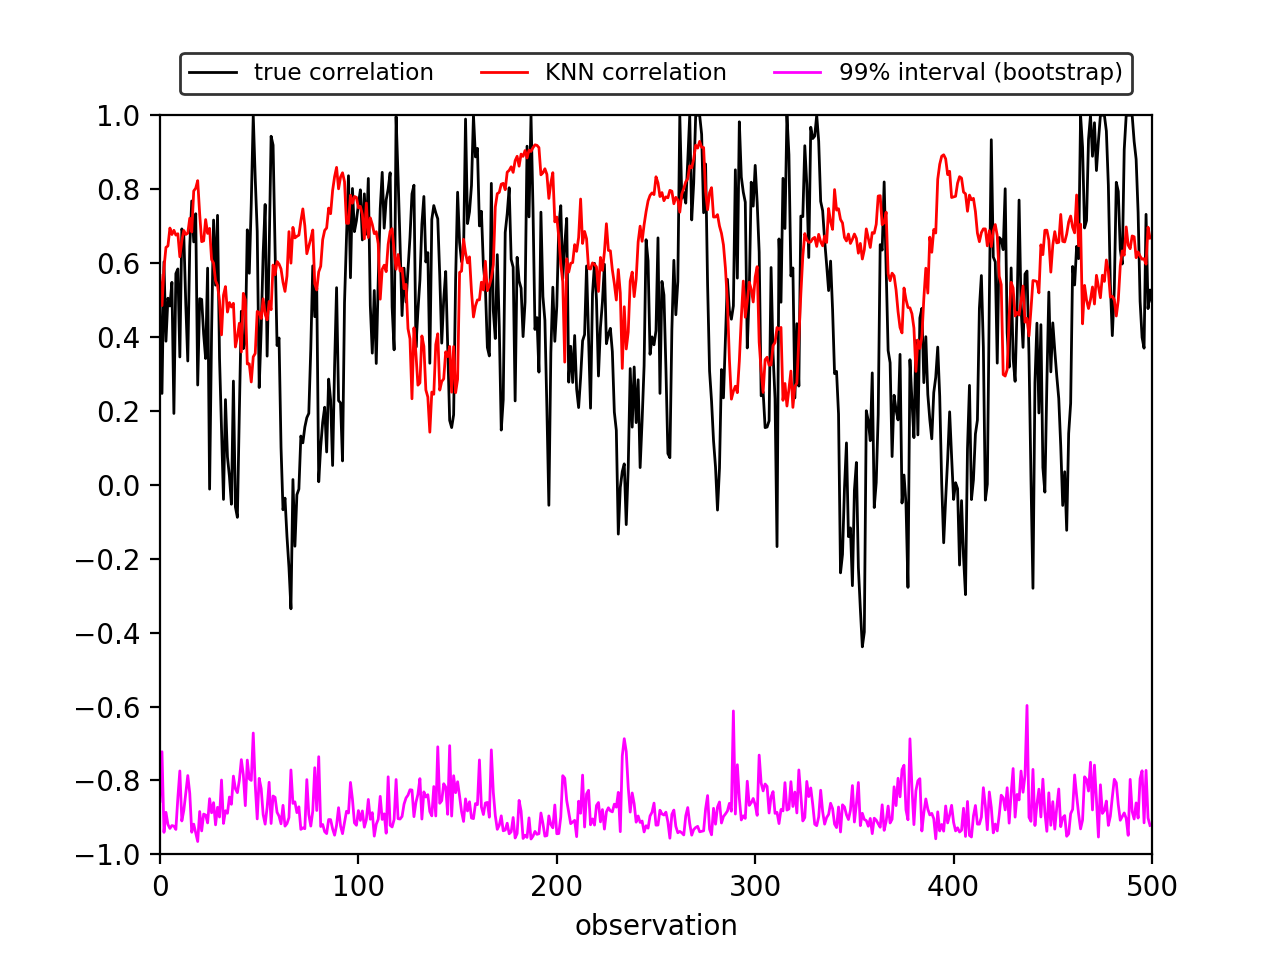
\includegraphics[width=\textwidth, height=0.5\textwidth]{knn_pearson_21_estimates_bootstrap_proxy.png} 
		\caption{KNN(5) estimates with $\Delta=21$, Pearson as covariate and proxy correlation.} 	
		\label{fig:knn_pearson21_bootstrap_proxy}
	\end{subfigure} 
	\hfill	
	\begin{subfigure}[b]{0.49 \textwidth} 
		\centering 
		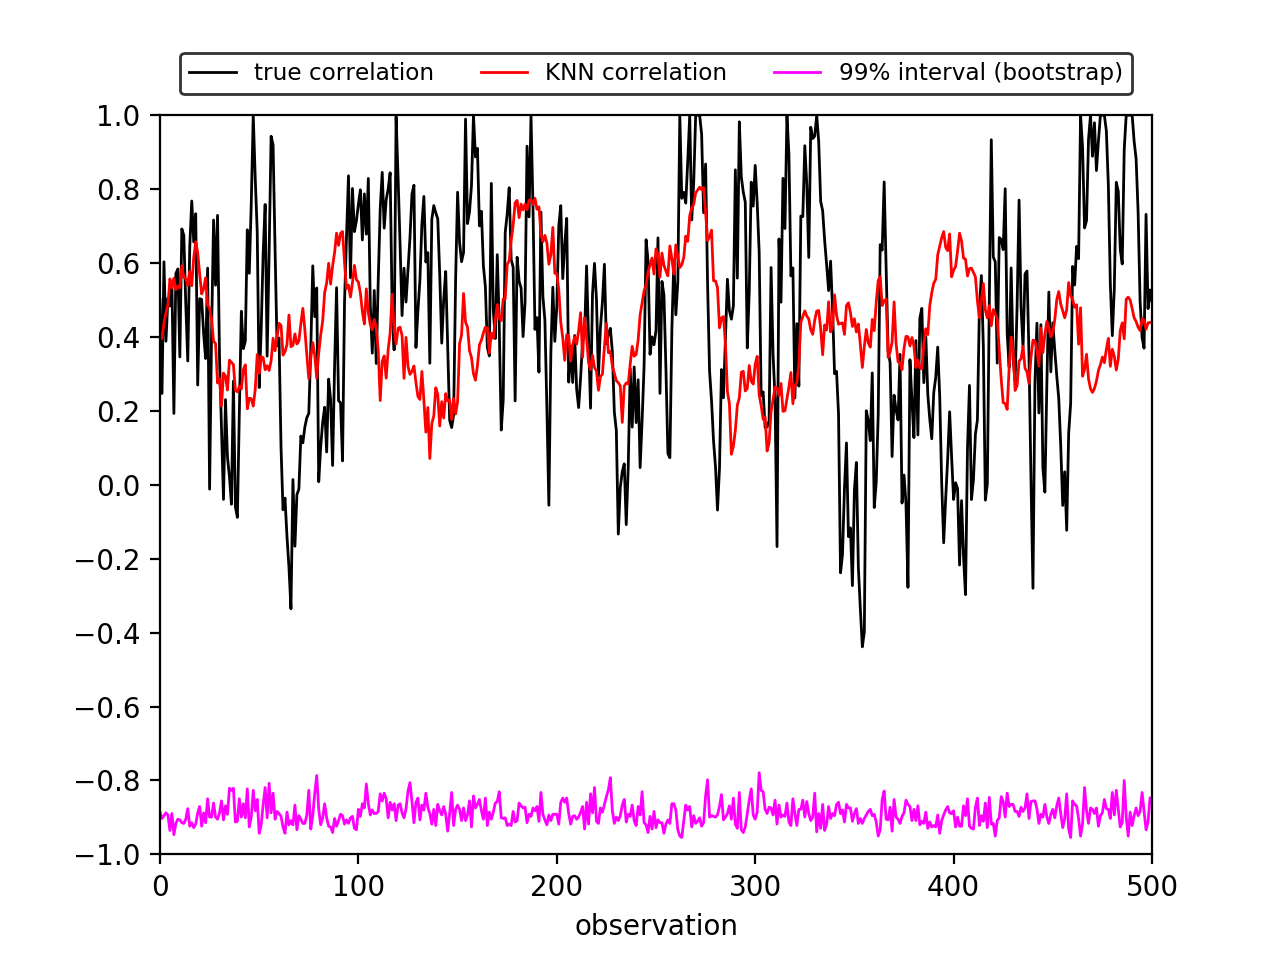
\includegraphics[width=\textwidth, height=0.5\textwidth]{knn_kendall_21_estimates_bootstrap_proxy.png} 
		\caption{KNN(5) estimates with $\Delta=21$, Kendall as covariate and proxy correlation.} 
		\label{fig:knn_kendall21_bootstrap_proxy}
	\end{subfigure} 
	\hfill	
	\begin{subfigure}[b]{0.49 \textwidth}
		\centering 
		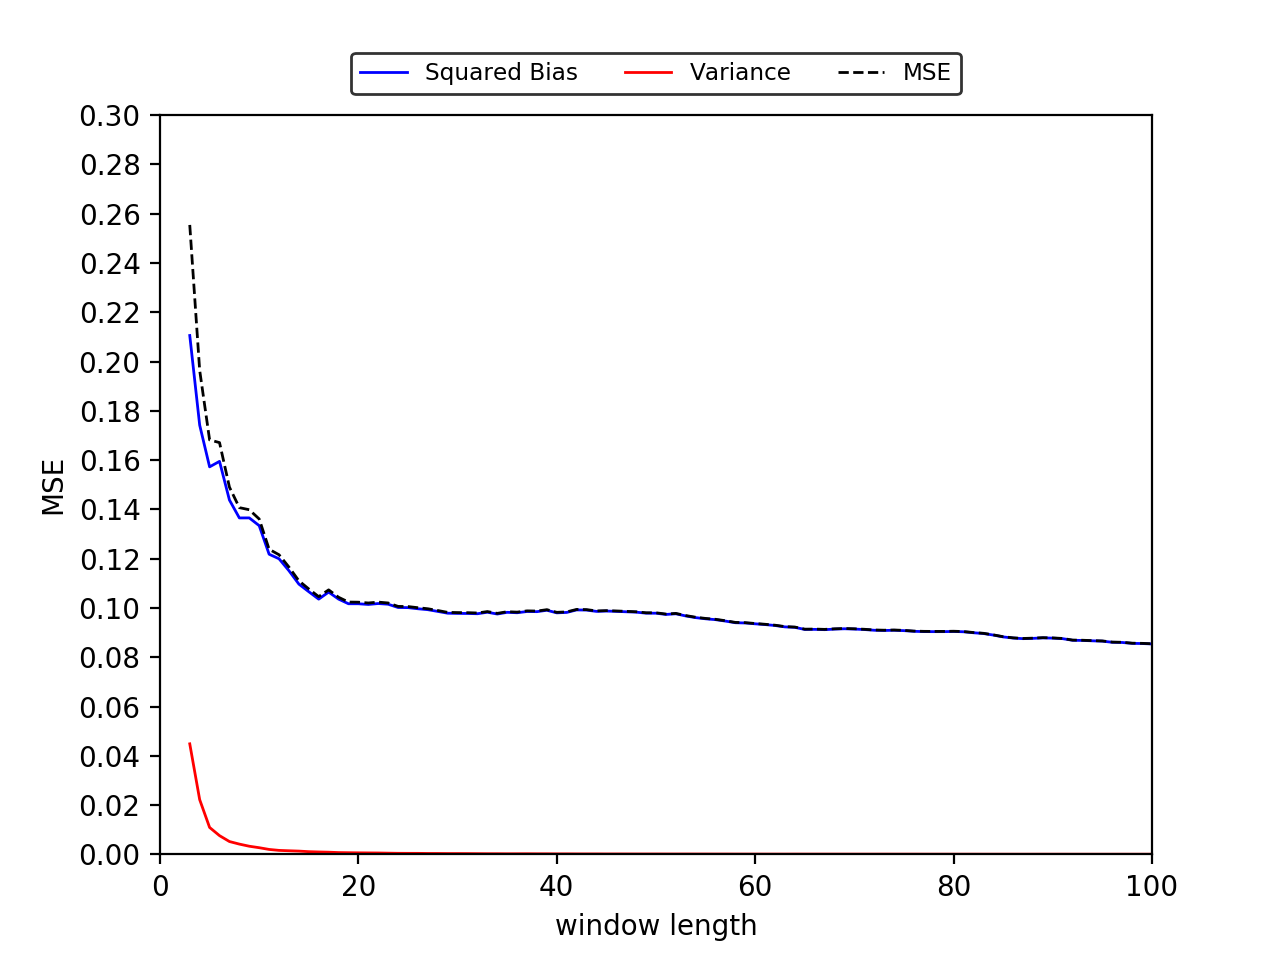
\includegraphics[width=\textwidth, height=0.5\textwidth]{decom_mse_knn_pearson_proxy.png} 
		\caption{Bias-variance decomposition for KNN(5) estimates with Pearson as covariate and proxy correlation.} 	
		\label{fig:decom_mse_knn_pearson_proxy}
	\end{subfigure}
	\hfill  
	\begin{subfigure}[b]{0.49 \textwidth}
		\centering 
		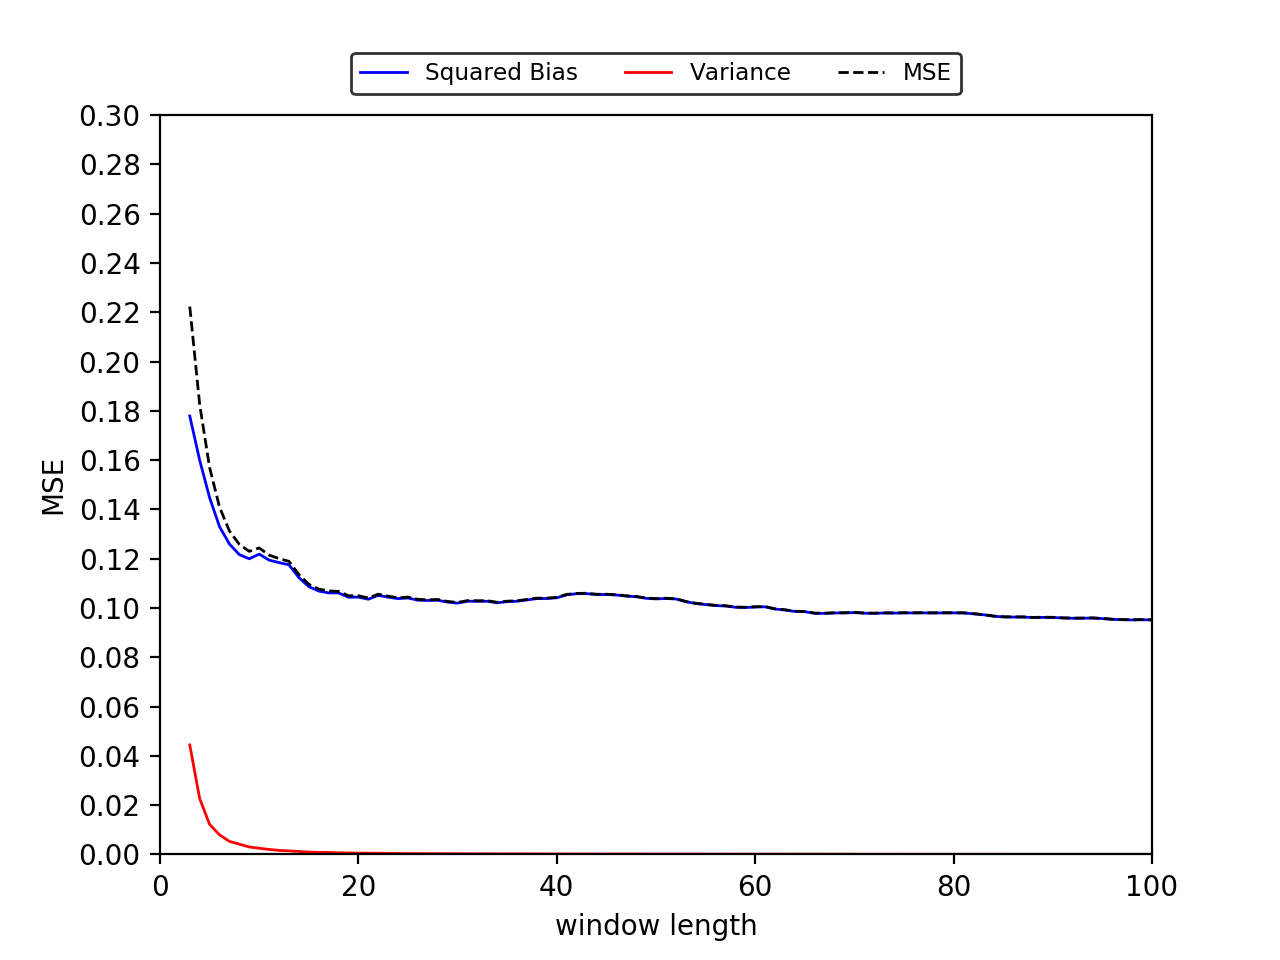
\includegraphics[width=\textwidth, height=0.5\textwidth]{decom_mse_knn_kendall_proxy.png} 
		\caption{Bias-variance decomposition for KNN(5) estimates with Kendall as covariate and proxy correlation.} 
		\label{fig:decom_mse_knn_kendall_proxy}
	\end{subfigure}
	\caption[MSE decomposition for KNN(5) under proxy correlation.]{MSE for KNN(5) estimates with Pearson and Kendall Moving Window bootstrap estimates as covariates and proxy correlation.}
	\label{fig:decom_mse_knn5_pearson_kendall_proxy}
\end{figure}


\subsection{Effect of Alternative Nearest Neighbor Parameterizations under Proxy Correlation} \label{sec:MSE_knn_alt_proxy}
Tabel \ref{tab:mse_decomp_knn_pearson_kendall_proxy} presents MSE decomposition as a function of number of neighbors $k$ for KNN estimators with approximations for both covariates and response variable. Similar results are observed for $k \in \{5, 10, 25, 50, 100\}$ when compared with KNN estimators with approximated covariates and true correlation in tabel \ref{tab:mse_decomp_knn_pearson_kendall_true}; both squared bias and variance initially decrease with an increase in $k$, and conversely, regardless whether the set of covariates is constructed from Pearson or Kendall correlation estimates using moving windows. Given our discussion from section \ref{sec:mse_decompose}, one might have expected an increase in squared bias with an increase in $k$. A possible explanation for this behavior may be that up to some $k$, an increase in $k$ implies additional neighbors containing informational value are used for estimation of conditional correlation. Logically, the inclusion of additional neighbors containing informational value yields more accurate estimates of correlation, that is, a decrease in squared bias. As of some $k$, however, additional neighbors only add noise to the estimation process, which translates into increased squared bias. Interestingly, Tabel \ref{tab:mse_decomp_knn_pearson_kendall_proxy} shows a slight increase in variance from $k = 800$ and $k = 900$ onwards for KNN estimates with Pearson and Kendall covariates, respectively. This may be due to sampling variation.           


%% TABLE
\begin{table}[H]
\centering
\captionsetup[subtable]{position=below}
%\captionsetup[table]{position=below}
\begin{subtable}{0.49\linewidth}
\centering
\begin{tabular}{r  c  c  c} 
\toprule
\multicolumn{1}{ r }{\textbf{k}} &
\multicolumn{1}{ c }{\textbf{Squared Bias}} &
\multicolumn{1}{ c }{\textbf{Variance}} &
\multicolumn{1}{ c }{\textbf{MSE}} \\
\midrule 

5                                     & 0.1334                         & 0.0027                & 0.1361     \\
10                                   & 0.1319                         & 0.0015                & 0.1334     \\
25                                   & 0.1289 	                    & 6.64e-4                & 0.1295     \\
50                                   & 0.1268                         & 3.57e-4                & 0.1271     \\
100                                 & 0.1238                         & 1.95e-4               & 0.1240      \\
200                                 & 0.1169                         & 1.14e-4               & 0.1170      \\
400                                 & 0.1047                         & 7.80e-5               & 0.1048      \\
600                                 & 0.0946                         & 7.20e-5               & 0.0947     \\
800                                 & 0.0870                         & 7.50e-5               & 0.0870      \\
900				     & 0.0841			   & 8.00e-5              & 0.0842      \\
1000                               & 0.0827                         & 8.80e-5              & 0.0828     \\ [1ex]
\bottomrule
\end{tabular}
\caption{MSE for KNN estimates with $\Delta=10$, Pearson as covariate and correlation.}
\label{tab:mse_decomp_knn_pearson_proxy}
\end{subtable}
\hfill
\begin{subtable}{0.49\linewidth}
\centering
\begin{tabular}{r  c  c  c} 
\toprule
\multicolumn{1}{ r }{\textbf{k}} &
\multicolumn{1}{ c }{\textbf{Squared Bias}} &
\multicolumn{1}{ c }{\textbf{Variance}} &
\multicolumn{1}{ c }{\textbf{MSE}} \\
\midrule 

5                                     & 0.1219                         &  0.0025              & 0.1244   \\
10                                   & 0.1200                         & 0.0014               & 0.1214   \\
25                                   & 0.1183	                   & 5.98e-4              & 0.1189    \\
50                                   & 0.1168                        & 3.17e-4	       & 0.1171    \\
100                                 & 0.1148                         & 1.75e-4              & 0.1150    \\
200                                 & 0.1110                        & 1.02e-4              & 0.1110    \\
400                                 & 0.1042                        & 6.80e-5             & 0.1043   \\
600                                 & 0.0998                         & 6.00e-5             & 0.0998     \\
800                                 & 0.0969                         & 5.90e-5             & 0.0970    \\
900				     & 0.0969			   & 6.00e-5             & 0.0970     \\
1000                               & 0.0988                       & 6.30e-5             & 0.0988     \\  [1ex]
\bottomrule
\end{tabular}
\caption{MSE for KNN estimates with $\Delta=10$, Kendall as covariate and correlation.}
\label{tab:mse_decomp_knn_kendall_proxy}
\end{subtable}
\caption{MSE decomposition as a function of the number of neighbors (k) for KNN with approximations for both covariates and response variable.}
\label{tab:mse_decomp_knn_pearson_kendall_proxy}
\end{table}

\noindent
Similar to section \ref{sec:MSE_knn_alt_true}, two more parameterizations of the KNN learning algorithm are analyzed where the set of neighbors used for point estimation of conditional correlation is defined as the entire training data set. The KNN estimators uses an uniformly weighted average of correlations, as defined in \eqref{eq:uni_weights}, and an inverse distance weighted average of correlations, as defined in \eqref{eq:inverse_weights}, which will be referred to as KNN(idw). However, the choice of an uniform distance weighting function results in approximately constant correlation, as depicted in figure \ref{fig:knn_pearson21_len_train_bootstrap_true} where the true correlation was considered as the response variable. The idea of assuming constant correlation is the concept we aim to improve on in this paper by considering correlation to be time-varying. As such, the remainder of this section will primarily focus on results from the KNN estimator considering an inverse distance weighting function, that is, KNN(idw). \\
  
\noindent
Figure \ref{fig:decom_mse_knn_IDW_pearson_kendall_proxy} presents MSE decomposition of KNN(idw) estimates with proxies for covariates and the response variable. The variance term becomes negligible small in case the set of neighbors used for point estimation of conditional correlation is defined as the entire training set. The variance depicted by the red line is barely observable in the bottom of figures \ref{fig:decom_mse_knn_IDW_pearson_proxy}-\ref{fig:decom_mse_knn_IDW_kendall_proxy}. This is in line with results presented in tabel \ref{tab:mse_decomp_knn_pearson_kendall_proxy} where the value of the variance term becomes negligible small for larger $k$, regardless whether the set of covariates is constructed from Pearson or Kendall sample correlation estimates using moving windows. Figures \ref{fig:knn_pearson_21_IDW_estimates_bootstrap_proxy}-\ref{fig:knn_kendall_21_IDW_estimates_bootstrap_proxy} show that the KNN(idw) estimator captures conditional correlation dynamics in a low volatile and smooth manner. When these plots are compared with the more volatile correlation dynamics estimated by the KNN(5) estimator, one can conclude the number of neighbors determines how active one wishes the algorithm to react to sudden changes in correlation. In practice, the underlying correlation dynamics may potentially be best captured optimizing over the hyperparmeter $k$ until an appropriate level of volatility and smoothness is found.         \\      




\begin{figure}[H]  % [h] parameter makes sure figures are located at 'this' location.
	\centering
	\begin{subfigure}[b]{0.49 \textwidth}
		\centering 
		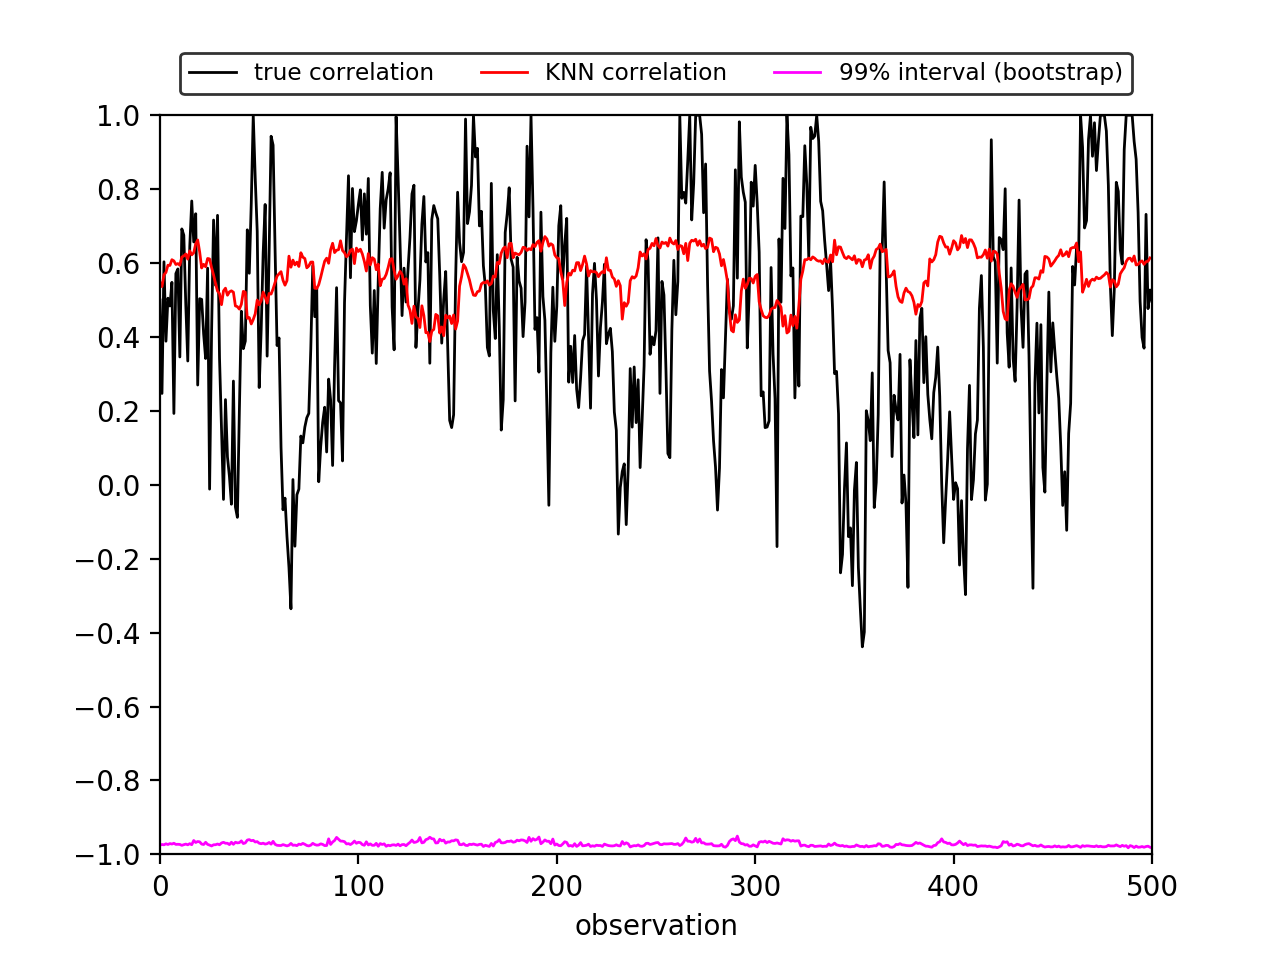
\includegraphics[width=\textwidth, height=0.5\textwidth]{knn_pearson_21_IDW_estimates_bootstrap_proxy.png} 
		\caption{KNN(idw) with $\Delta=21$ and Pearson covariates.} 	
		\label{fig:knn_pearson_21_IDW_estimates_bootstrap_proxy}
	\end{subfigure}
	\hfill  
	\begin{subfigure}[b]{0.49 \textwidth}
		\centering 
		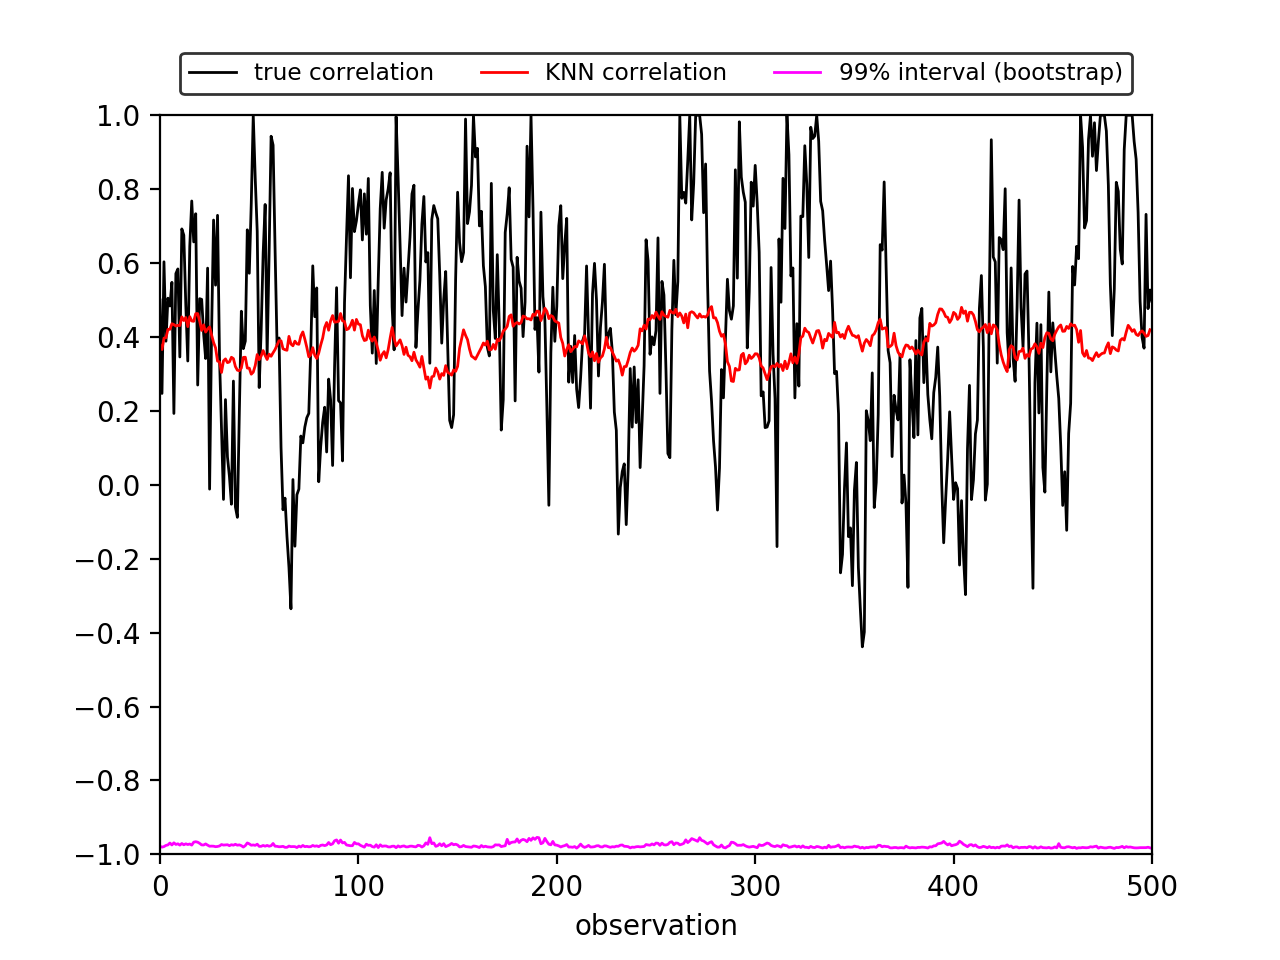
\includegraphics[width=\textwidth, height=0.5\textwidth]{knn_kendall_21_IDW_estimates_bootstrap_proxy.png} 
		\caption{KNN(idw) with $\Delta=21$ and Kendall covariates.} 
		\label{fig:knn_kendall_21_IDW_estimates_bootstrap_proxy}
	\end{subfigure}
	\hfill  
	\begin{subfigure}[b]{0.49 \textwidth}
		\centering 
		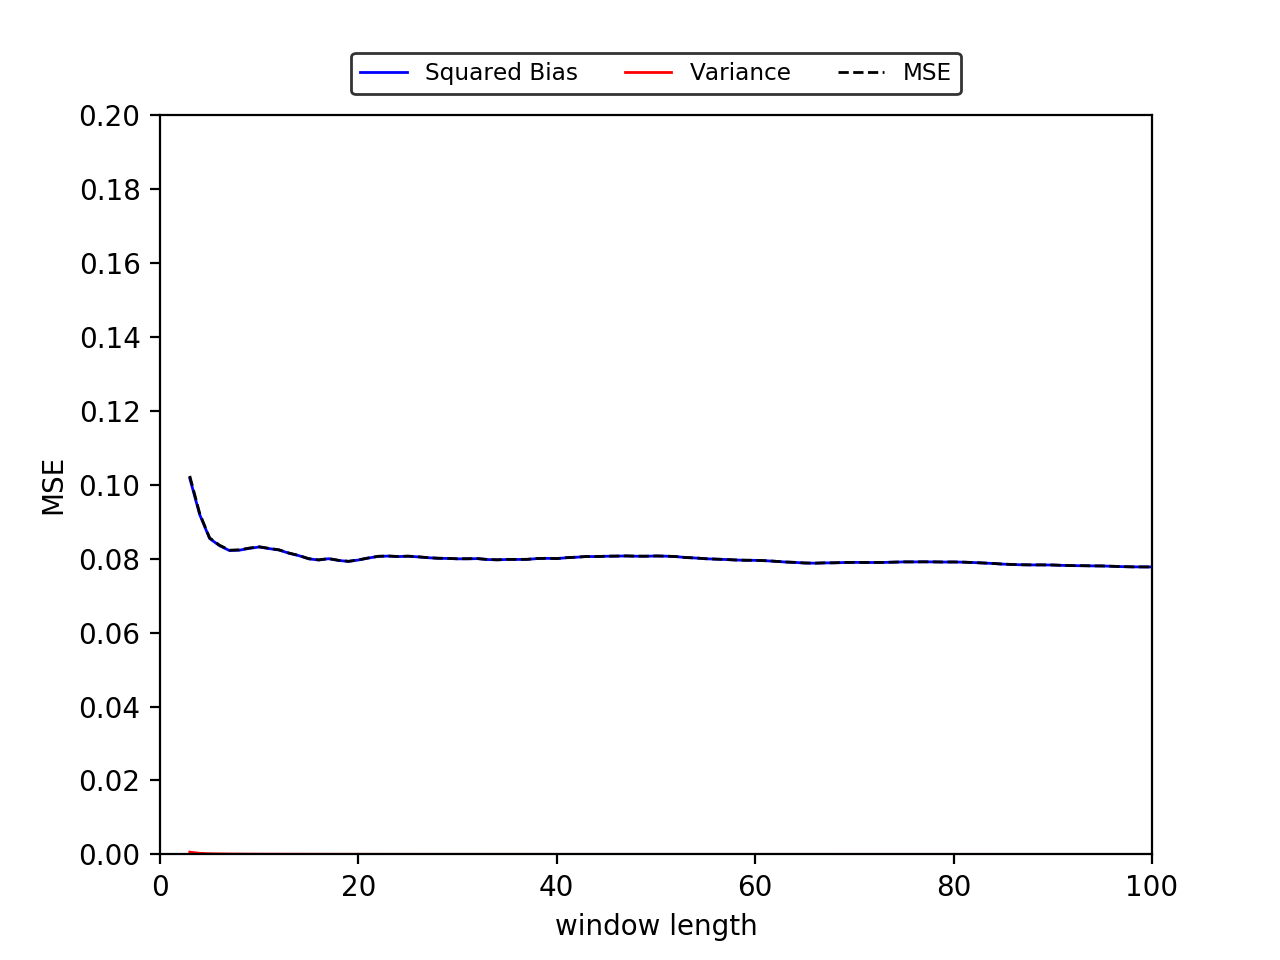
\includegraphics[width=\textwidth, height=0.5\textwidth]{decom_mse_knn_IDW_pearson_proxy.png} 
		\caption{Bias-variance decomposition for KNN(idw) estimates with Pearson as covariate.} 
		\label{fig:decom_mse_knn_IDW_pearson_proxy}
	\end{subfigure}
	\hfill  
	\begin{subfigure}[b]{0.49 \textwidth}
		\centering 
		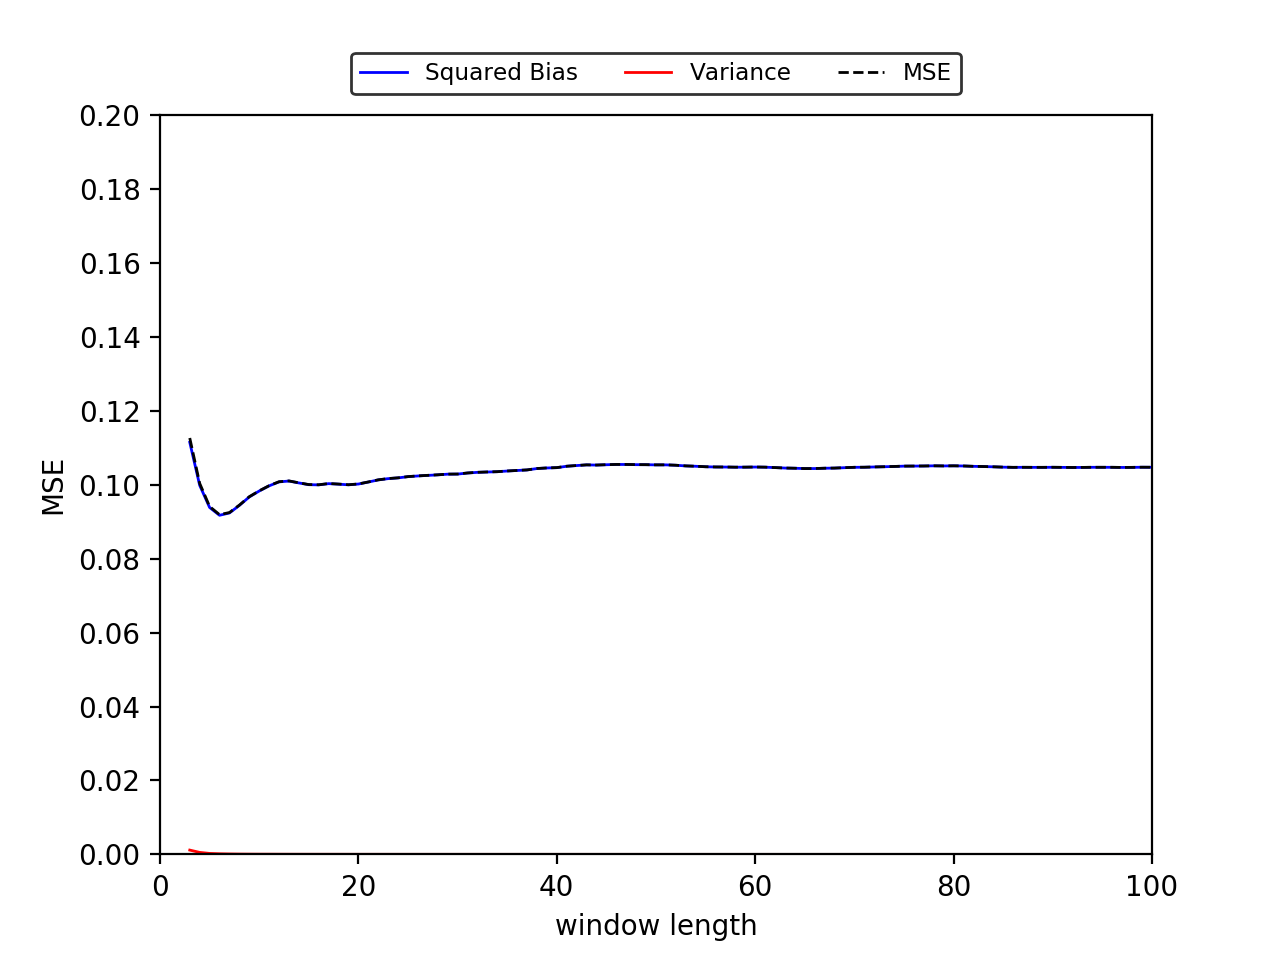
\includegraphics[width=\textwidth, height=0.5\textwidth]{decom_mse_knn_IDW_kendall_proxy.png} 
		\caption{Bias-variance decomposition for KNN(idw) estimates with Kendall as covariate.} 
		\label{fig:decom_mse_knn_IDW_kendall_proxy}
	\end{subfigure}
	\caption[MSE decomposition for KNN(idw) under proxy correlation.]{MSE for KNN(idw) with Pearson and Kendall Moving Window bootstrap estimates as covariates and response variable.}
	\label{fig:decom_mse_knn_IDW_pearson_kendall_proxy}
\end{figure}


\noindent
Regardless of the choice of window length, MSE from KNN(unif) and the set of covariates and response variable constructed from Pearson and Kendall sample correlation estimates using moving windows are approximately between 0.0774 and 0.0923, and 0.1054 and 0.1118, respectively. MSE from KNN(idw) is approximately between 0.0778 and 0.1024, and between 0.0919 and 0.1127, respectively. This implies that, using a KNN estimator, approximations based on Pearson sample correlations using moving windows seems more appropriate for the simulated data from \eqref{eq:correlation_simulation} than Kendall sample correlations using moving windows, regardless of the weighting function; figure \ref{fig:decom_mse_knn_IDW_pearson_proxy} depicts a lower MSE for all window sizes compared with MSE in figure \ref{fig:decom_mse_knn_IDW_kendall_proxy}. An explanation for this observation is given along the same lines as for Pearson and Kendall sample correlation estimates using moving windows in section \ref{sec:true_correlation}; the simulated asset returns follow a multivariate normal distribution, that is, an elliptical distribution. Therefore, it makes sense that lower MSE values may be obtained when true correlation is approximated in an KNN estimator using a linear correlation coefficient such as Pearson. Furthermore, the choice for an inverse distance weighting function seems to have no significant performance advantage, in terms of MSE, over an uniform weighting function when true correlation is approximated using moving window estimates. Interestingly, this is in contrast with results obtained from KNN estimator under true correlation in section \ref{sec:MSE_knn_true}. Note, however, that using a uniform weighting function with the entire training set yields approximately constant correlation estimates, which is the exact concept we aim to improve on with a more realistic assumption of conditional correlation. Latter is better captured under an inverse distance weighting function. Finally, the variance of MSE from KNN(unif) and the set of covariates constructed from Pearson and Kendall moving window estimates are approximately 3.98e-6 and 9.26e-7, respectively. The variance of MSE from KNN(idw) and the set of covariates constructed from Pearson and Kendall moving window estimates are approximately 8.46e-6 and 8.61e-6, respectively. The difference in sensitivity to the choice of window length between the different parameterizations is negligible small if significant at all. Lastly, figure \ref{fig:det_knn_len_train_IDW_pearson_kendall_proxy} presents the obtained minimum determinants of $R_t$ for all considered choices of window length under the proposed alternative parameterizations; the alternative parameterizations of the KNN estimator also satisfy the positive semidefiniteness condition in the conditional correlation matrix $R_t$ for the entire out-of-sample period under all considered choices of window.\\

\noindent 
This section is concluded with a comparison of the function approximation capabilities of the KNN estimator and Pearson and Kendall sample correlation estimates using moving windows. Comparison is based on MSE between estimated and true correlations. Figure \ref{fig:mse_knn5_IDW_pearson_kendall_proxy}\footnote{Only behavior of the (alternative parameterized) KNN estimator with Pearson covariates is shown as behavior of its Kendall counterpart is nearly identical.} shows MSE from KNN(5), an alternative parameterization with an inverse distance weighting function, KNN(idw), and Pearson and Kendall sample correlation estimates. According to MSE, parameterizations of the KNN estimator with approximated correlations performs significantly better than those of Pearson and Kendall moving window estimates for small window sizes. Moreover, the KNN(idw) yields significantly smaller MSE compared to Pearson and Kendall moving window estimates for all window sizes. Thus, similar to the analysis in section \ref{sec:MSE_knn_alt_true}, the KNN estimator yields lower MSE with an increase in the number of neighbors, particularly for smaller window sizes. This result follows from the fact that estimated conditional correlation is based on increased sample information, which positively contributes to accurately capturing time-varying dynamics in correlation. Evidently, underlying correlation dynamics may potentially be best captured optimizing over the hyperparmeter $k$ until a preferred level of volatility and smoothness is reached. Finally, the variance of MSE from KNN(5) estimates and KNN(idw) in figure \ref{fig:mse_knn5_IDW_pearson_kendall_proxy} are 5.70e-4 and 8.46e-6, respectively, while that of Pearson and Kendall sample correlation estimates are 0.0040 and 0.0037, respectively. In other words, the KNN estimator with approximated covariates and response variable is significantly less sensitive to the choice of window length than Pearson and Kendall sample correlation estimates.  \\



\begin{figure}[H] 
	\centering
	\begin{subfigure}[b]{0.49 \textwidth}
		\centering 
		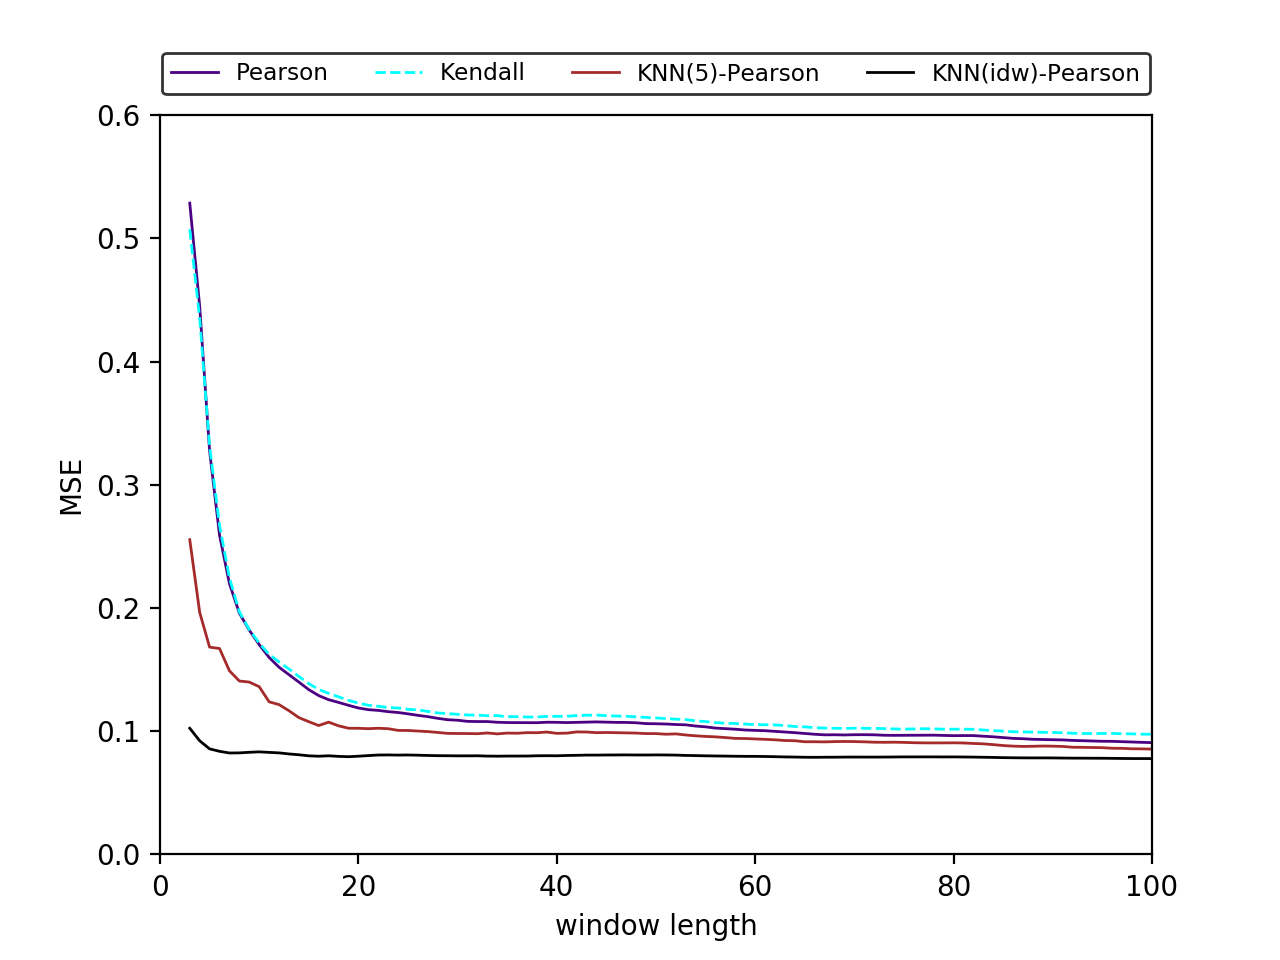
\includegraphics[width=\textwidth, height=0.5\textwidth]{mse_knn5_IDW_pearson_kendall_proxy} 
		\caption{MSE for KNN with Pearson covariates and proxy correlation, Pearson and Kendall Moving Window bootstrap estimates.}
		\label{fig:mse_knn5_IDW_pearson_kendall_proxy}
	\end{subfigure}
	\hfill
	\begin{subfigure}[b]{0.49 \textwidth} 
		\centering
		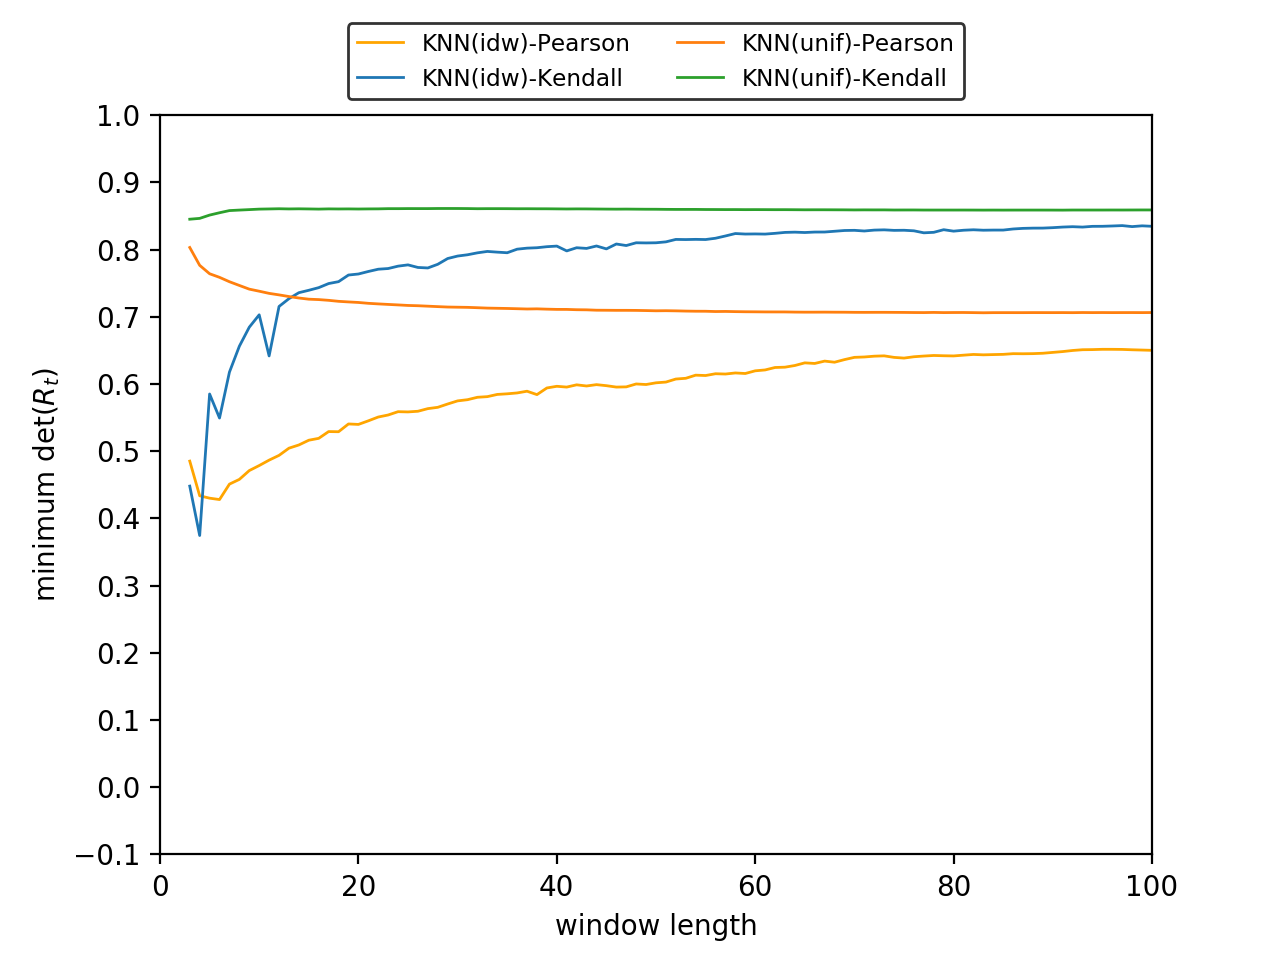
\includegraphics[width=\textwidth, height=0.5\textwidth]{det_knn_IDW_len_train_pearson_kendall_proxy}
		\caption{Minimum determinants for KNN(idw) and KNN(unif) estimates with Pearson and Kendall covariates and proxy correlation.}
		\label{fig:det_knn_len_train_IDW_pearson_kendall_proxy}
	\end{subfigure}	
	\caption[MSE and minimum determinants for KNN under proxy correlation,  Pearson and Kendall Moving Window bootstrap estimates.]{Comparison MSE and minimum determinants for KNN with Pearson covariates and proxy correlation, Pearson and Kendall Moving Window bootstrap estimates.}
	\label{mse_det_knn5_IDW_pearson_kendall_proxy}
\end{figure}



%%%%%%% RANDOM FOREST PROXY %%%%%%%%%%%%%%
\subsection{Generalization Error of Random Forest under Proxy Correlation} \label{sec:MSE_rf_proxy}
The accuracy of RF estimates with Pearson and Kendall covariates for conditional correlation is compared in terms of the MSE between estimated and true correlations. MSE from RF(1) with Pearson and Kendall moving window approximations for covariates and response variable are shown in figure \ref{fig:mse_rf10_pearson_kendall_proxy}. Regardless of the choice of window length, MSE from RF(10) with Pearson and Kendall covariates are between 0.0868 and 0.2318, and 0.0946 and 0.2321, respectively. The variance of MSE from RF(10) estimates with Pearson covariates is approximately 4.54e-4 while that of RF(10) estimates with Kendall covariates is approximately 3.23e-4. Interestingly, figure \ref{fig:mse_rf10_pearson_kendall_proxy} shows that MSE from RF(10) estimation with approximated response variable varies substantially for smaller window sizes. Although, less variation is observed when compared with MSE from Pearson and Kendall sample correlation estimates using moving windows depicted in figure \ref{fig:mse_pearson_kendall_bootstrap}. This observation is analogous to the comparison of KNN(5) estimates of correlation. 

\begin{figure}[H]
	\centering
	\begin{subfigure}[b]{0.49 \textwidth} 
		\centering
		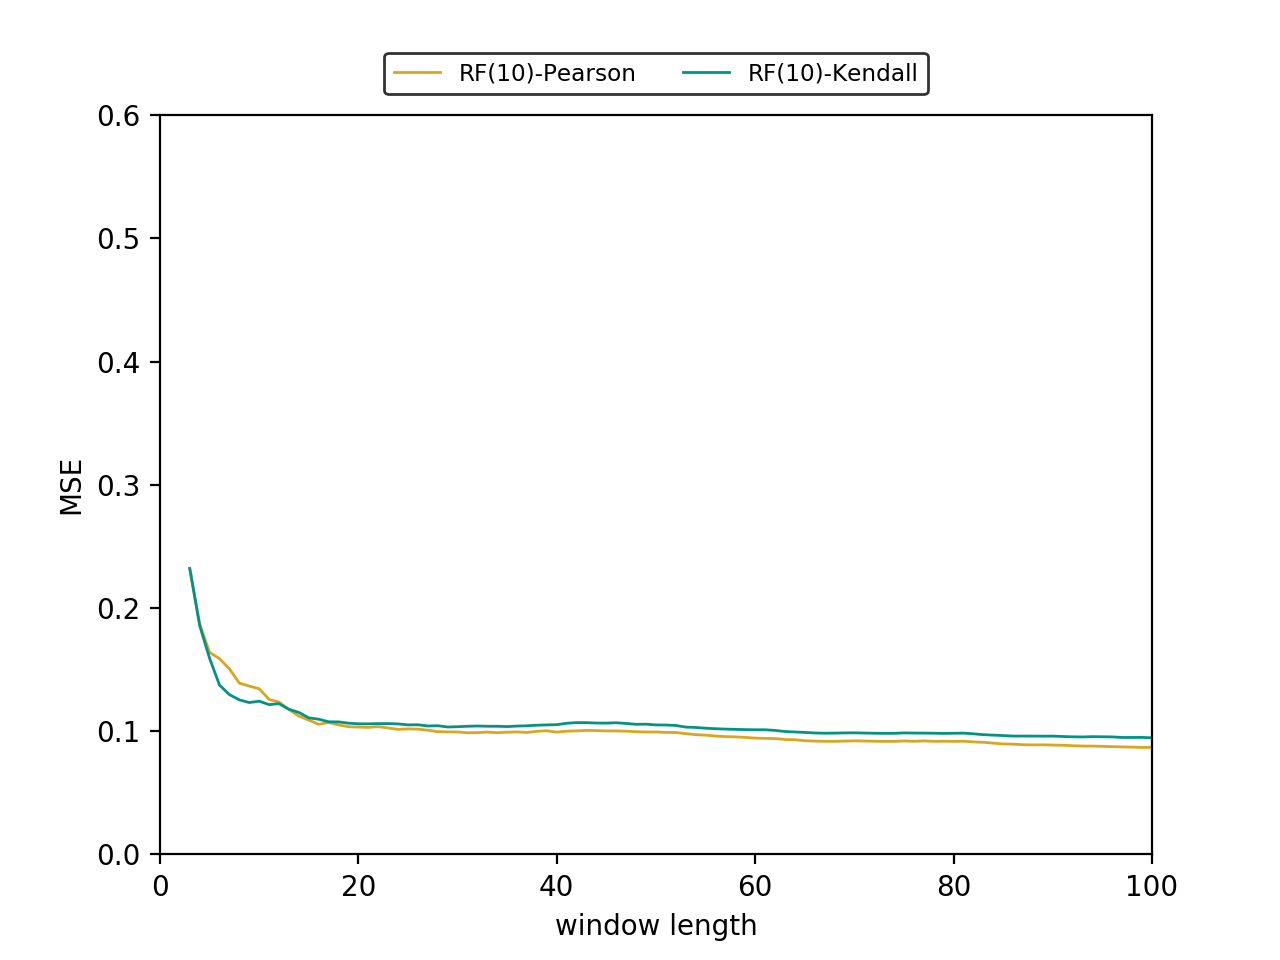
\includegraphics[width=\textwidth, height=0.5\textwidth]{mse_rf10_pearson_kendall_proxy}
		\caption{MSE for RF(10) with covariates from Pearson and Kendall and proxy correlation.}
		\label{fig:mse_rf10_pearson_kendall_proxy}
	\end{subfigure}
	\hfill
	\begin{subfigure}[b]{0.49 \textwidth} 
		\centering
		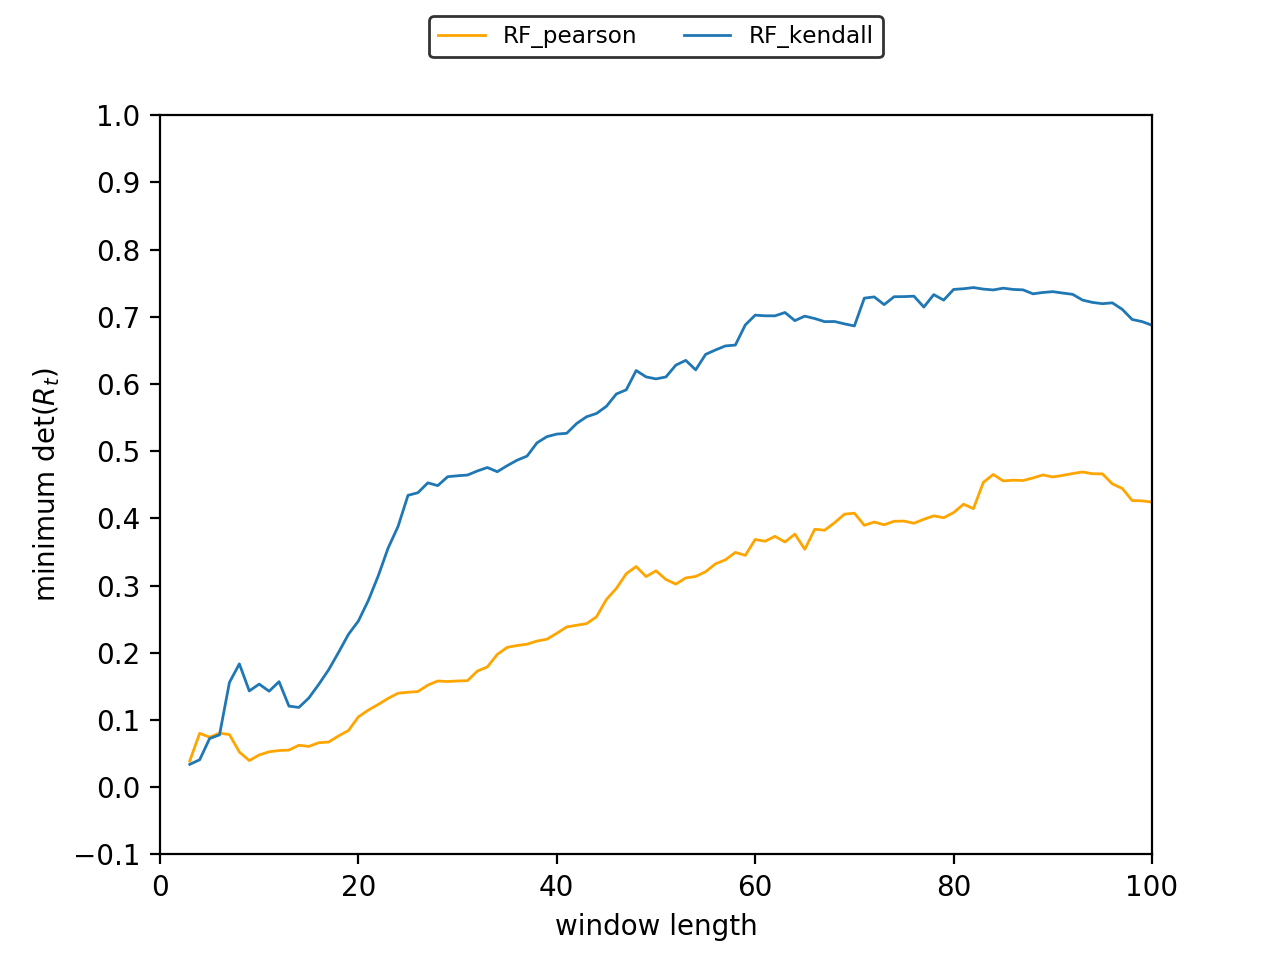
\includegraphics[width=\textwidth, height=0.5\textwidth]{det_rf10_pearson_kendall_proxy}
		\caption{Minimum determinants for RF(10) with covariates from Pearson and Kendall and proxy correlation.}
		\label{fig:det_rf10_pearson_kendall_proxy}
	\end{subfigure}
	\caption[MSE and minimum determinants for RF(n\_trees=10) under proxy correlation.]{Comparison MSE and minimum determinants for RF(n\_trees=10) with covariates from Pearson and Kendall and proxy correlation.}
	\label{fig:mse_det_rf10_pearson_kendall_proxy}
\end{figure}

\noindent
Figure \ref{fig:det_rf10_pearson_kendall_proxy} presents obtained minimum determinants of $R_t$ for all choices of window length. Although the minimum determinants for smaller window sizes approach 0, they remain nonnegative for the entire out-of-sample period; thus, RF(10) estimates of conditional correlation where both the set of covariates and response variable is constructed from Pearson and Kendall sample correlation estimates using moving windows satisfy the positive semidefiniteness condition in the conditional correlation matrix $R_t$ for the entire out-of-sample period. \\

\noindent
Visual inspection of the plots in figures \ref{fig:rf_pearson21_bootstrap_proxy}-\ref{fig:rf_kendall21_bootstrap_proxy} results into an analysis similar to the analysis of the KNN estimator under approximations of correlation instead of actual correlation in section \ref{sec:MSE_knn_proxy}. It is clear that the uncertainty in estimated conditional correlation $\rho_t$, which is illustrated by the 99\% confidence interval, is smaller for RF(10) estimates compared to Pearson and Kendall sample correlation estimates using moving windows, even though both the set of covariates and the response variable of the RF estimator are now based on approximations of correlation instead of true correlation. These figures also show smaller uncertainty in the conditional correlation, $\rho_t$, when compared with RF(10) estimates with true correlation as the response variable, which are depicted in figure \ref{fig:decom_mse_rf10_pearson_kendall_true}. Moreover RF(10) estimates of correlation with true correlation as response variable in figures \ref{fig:rf_pearson21_bootstrap_true}-\ref{fig:rf_kendall21_bootstrap_true} are much more volatile. In contrast, RF(10) estimates with approximated correlation as response variable in figures \ref{fig:rf_pearson21_bootstrap_proxy}-\ref{fig:rf_kendall21_bootstrap_proxy} follow the increases and decreases of the true correlation smoother, with tighter confidence intervals. This is a more desirable result as it is not expected that correlation between assets changes that drastically at each time unit. \\

\noindent
Figures \ref{fig:rf_pearson21_bootstrap_proxy}-\ref{fig:decom_mse_rf10_pearson_proxy} present MSE decomposition into bias and variance terms from RF(10) estimates of correlation. These figures indicate that the RF(10) estimator with approximated response variable is more sensitive to the choice of the window length for smaller window sizes compared to RF(10) estimator with true correlation depicted in figure \ref{fig:decom_mse_rf10_pearson_kendall_true}. This observation is similar to the observation when comparing the KNN estimators with different specifications of the response variable and can be explained by the propagation of approximation error in the response variable. Figures \ref{fig:decom_mse_rf10_pearson_proxy}-\ref{fig:decom_mse_rf10_kendall_proxy} show, however, that the RF(10) estimator with approximated response variable is considerably less sensitive to the choice of the window length for smaller window sizes when compared to Pearson and Kendall sample correlation estimates using moving windows depicted in figures \ref{fig:decom_mse_pearson}-\ref{fig:decom_mse_kendall}, respectively. Thus, analogous to the KNN estimator with approximated covariates and response variable, the RF estimator seems to mitigate the error propagation to some extend for smaller window sizes. Finally, a lower bias compared to Pearson and Kendall sample correlation estimates using moving windows implies a random forest may be more adequate as an estimator of conditional correlation between financial returns. Moreover, lower variance is observed when compared with Pearson and Kendall sample correlation estimates using moving windows. This can be accredited to the bootstrap aggregating procedure underlying the RF algorithm as explained in section \ref{sec:bagging}.        



\begin{figure}[H]  % [h] parameter makes sure figures are located at 'this' location.
	\centering
	\begin{subfigure}[b]{0.49 \textwidth} % sum of widths should be less than text width if all one the same line
		\centering 
		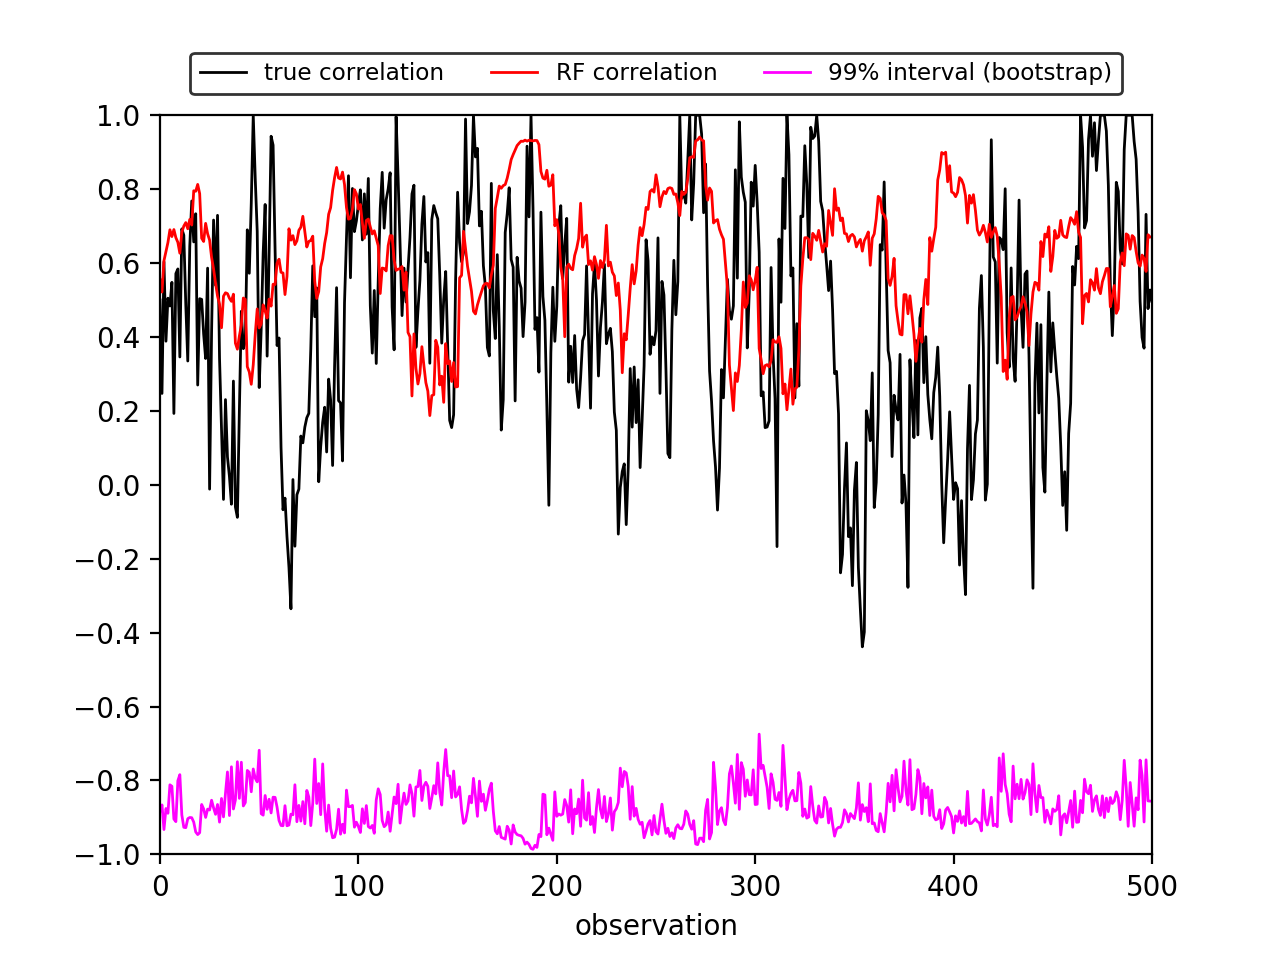
\includegraphics[width=\textwidth, height=0.5\textwidth]{rf_pearson_21_estimates_bootstrap_proxy.png} 
		\caption{RF(10) estimates with $\Delta=21$, Pearson as covariate and proxy correlation.} 	
		\label{fig:rf_pearson21_bootstrap_proxy}
	\end{subfigure} 
	\hfill	
	\begin{subfigure}[b]{0.49 \textwidth} 
		\centering 
		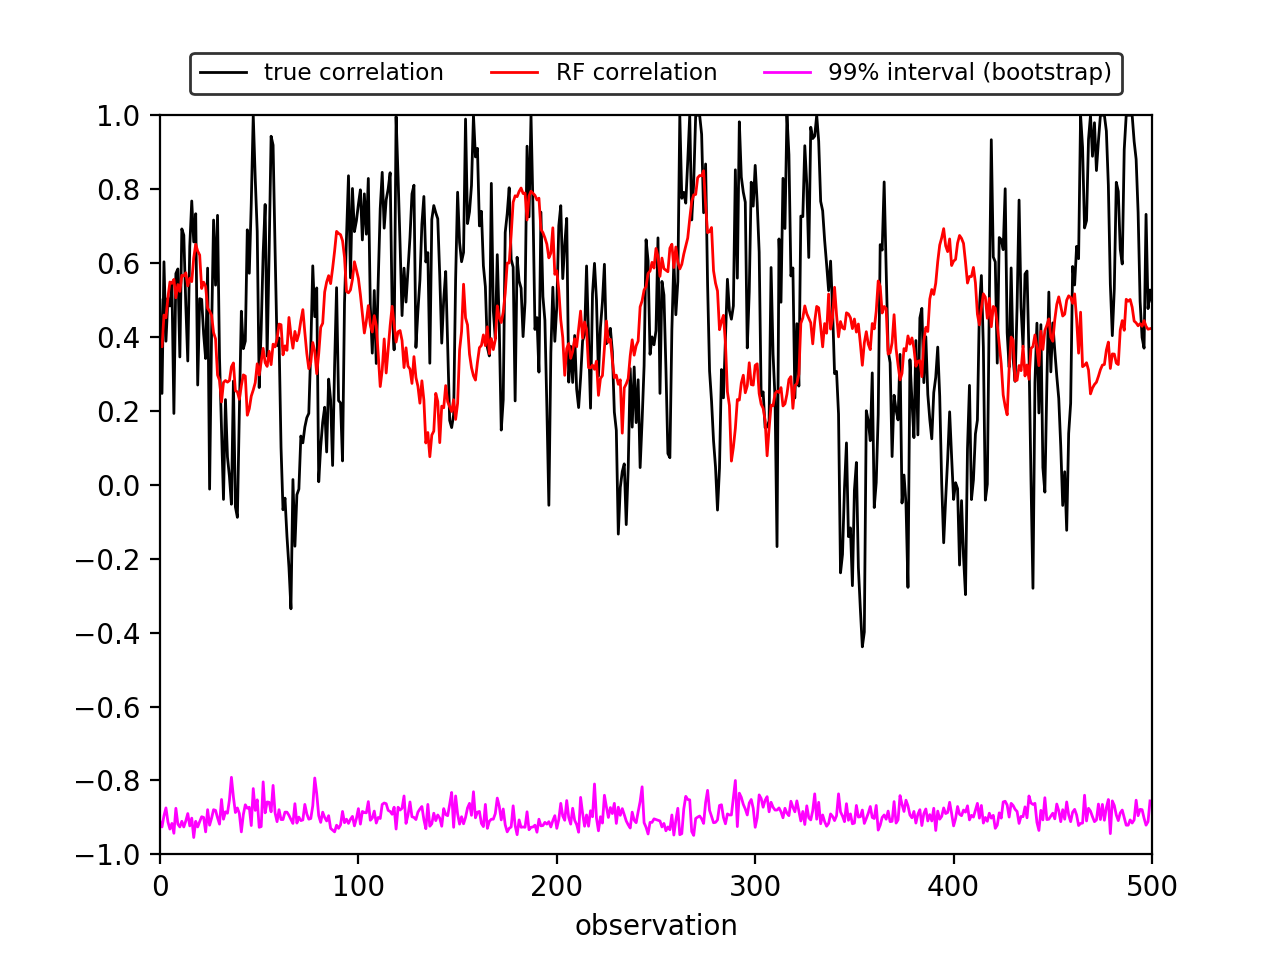
\includegraphics[width=\textwidth, height=0.5\textwidth]{rf_kendall_21_estimates_bootstrap_proxy.png} 
		\caption{RF(10) estimates with $\Delta=21$, Kendall as covariate and proxy correlation.} 
		\label{fig:rf_kendall21_bootstrap_proxy}
	\end{subfigure} 
	\hfill	
	\begin{subfigure}[b]{0.49 \textwidth}
		\centering 		
		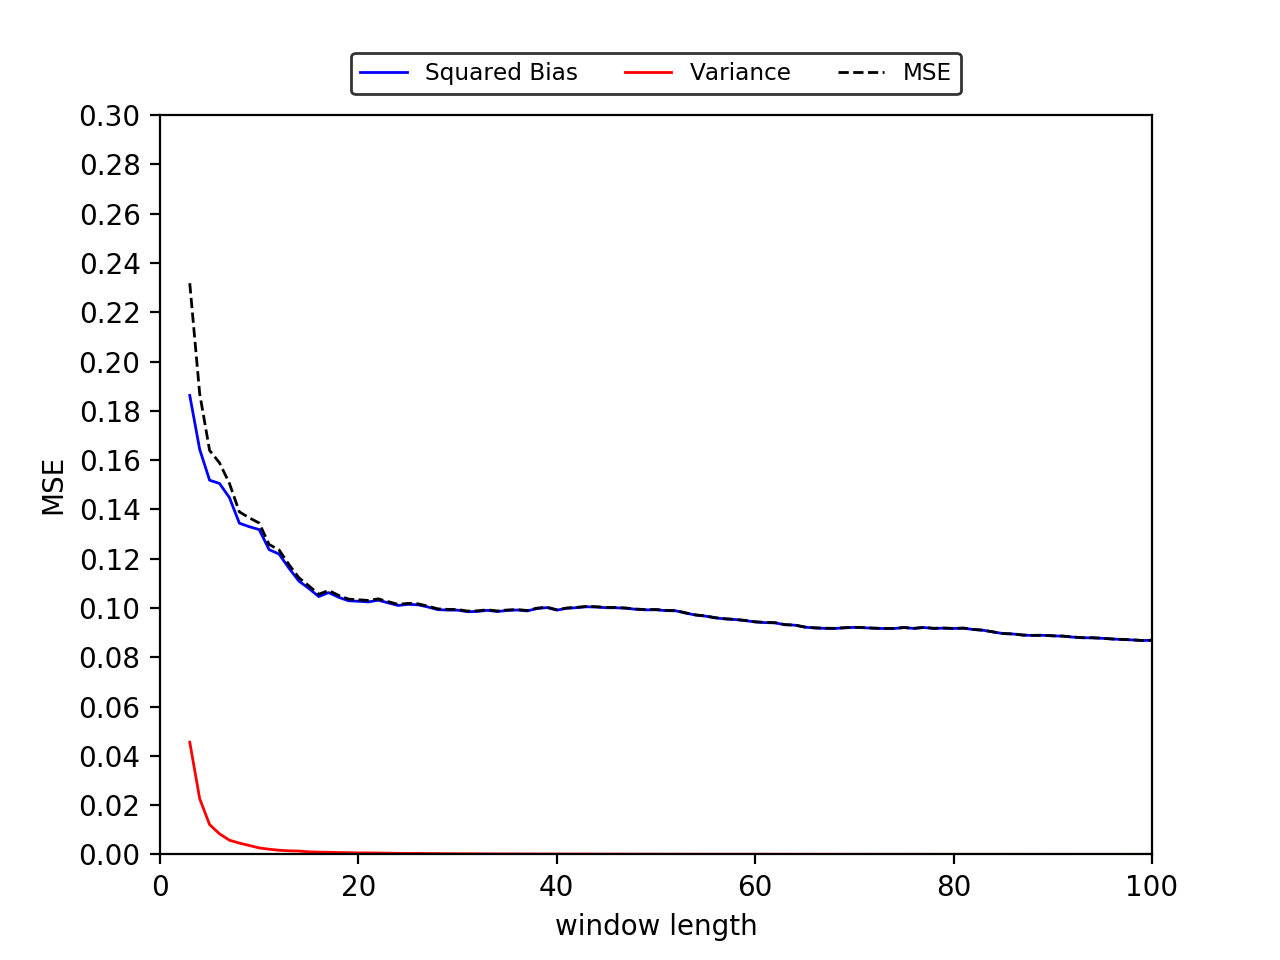
\includegraphics[width=\textwidth, height=0.5\textwidth]{decom_mse_rf10_pearson_proxy.png} 
		\caption{Bias-variance decomposition for RF(10) estimates with Pearson as covariate and proxy correlation.} 
		\label{fig:decom_mse_rf10_pearson_proxy}
	\end{subfigure}
	\hfill  
	\begin{subfigure}[b]{0.49 \textwidth}
		\centering 
		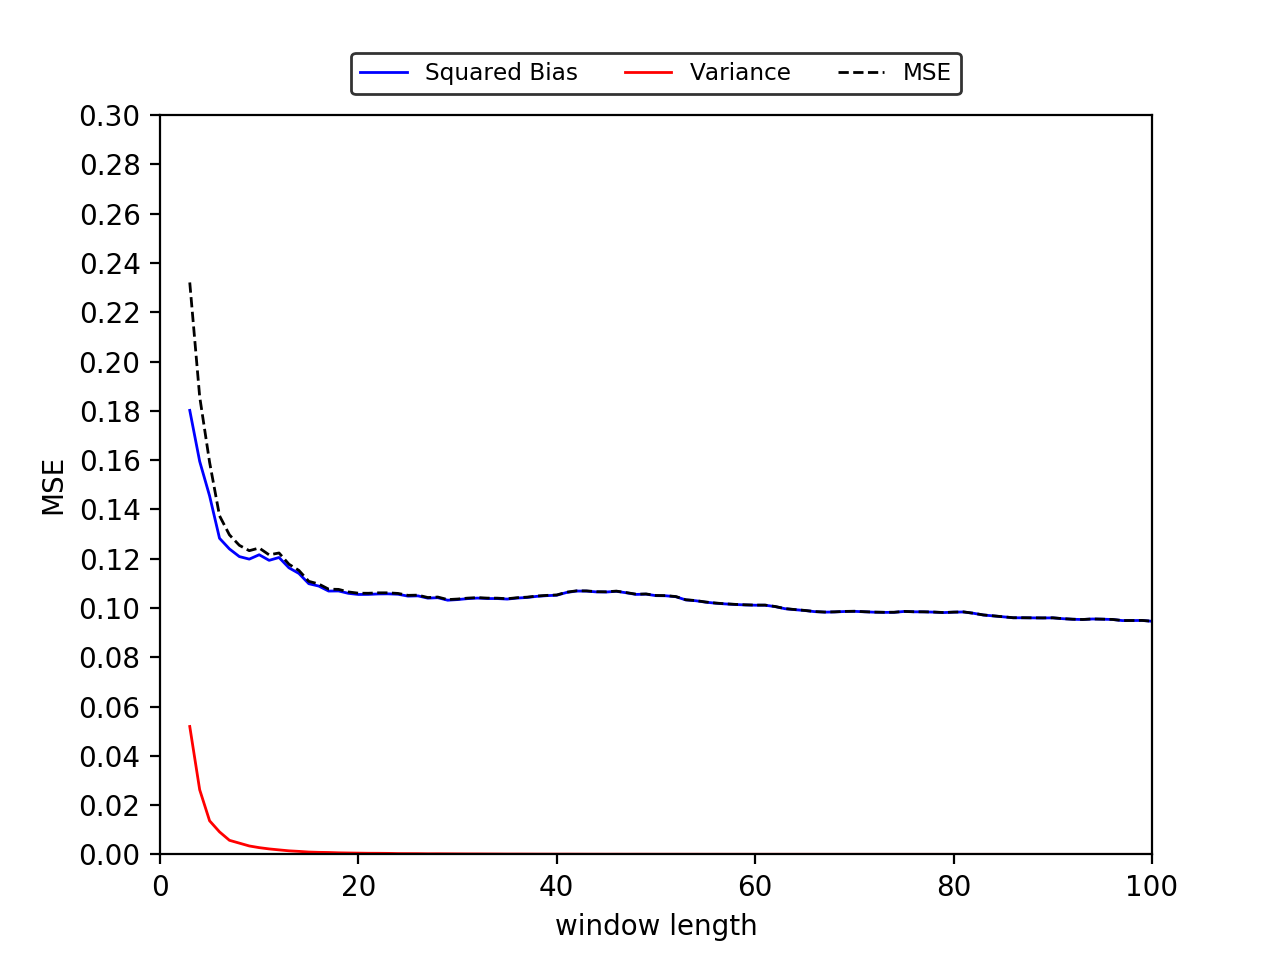
\includegraphics[width=\textwidth, height=0.5\textwidth]{decom_mse_rf10_kendall_proxy.png} 
		\caption{Bias-variance decomposition for RF(10) estimates with Kendall as covariate and proxy correlation.} 
		\label{fig:decom_mse_rf10_kendall_proxy}
	\end{subfigure}
	\caption[MSE decomposition for RF(10) estimates under proxy correlation.]{MSE for RF(10) estimates with Pearson and Kendall Moving Window bootstrap estimates as covariates and proxy correlation.}
	\label{fig:decom_mse_rf10_pearson_kendall_proxy}
\end{figure}

\subsection{Effect of Alternative Random Forest Parameterizations under Proxy Correlation} \label{sec:MSE_rf_alt_proxy}
Simulation results in tabel \ref{tab:mse_decomp_rf_pearson_kendall_proxy}\footnote{Results were obtained by taking 100 bootstrapped samples instead of 1000 due to computational time constraints. This number of bootstrapped samples is however sufficient for illustrational purposes.} show an inverse relationship between the number of decision trees in the random forest and the uncertainty around the estimated correlations, regardless whether Pearson or Kendall approximations are used for true correlation. It is clearly observed that an increase in the number of trees yields a decrease of the variance, and conversely. This observation is in line with our discussion on MSE decomposition for the RF estimator in section \ref{sec:mse_decompose}. 
For the correlation dynamics generated by \eqref{eq:correlation_simulation}, it is observed that the point of diminishing reduction in variance is reached with a smaller amount of trees compared with the sensitivity analysis of the random forest specified with true correlation as the response variable. \\

\noindent
With respect to our discussion on the effect of random covariate selection in individual tree construction on the squared bias and variance (section \ref{sec:mse_decompose}): the individual decision trees of the random forest in our simulation study are merely decision stumps as the dimension of the covariate set is only three (minimum and maximum returns and pairwise correlation of the previous time unit), that is, $P=3$, which means under default randomization for regression problems $p=P/3 = 1$. As such, no sensitivity analysis is undertaken on the number of covariates given the small dimension of the covariate set. This may, however, be interesting in high dimensional systems of correlations. \\  


%% TABLE
\begin{table}[H]
\centering
\captionsetup[subtable]{position=below}
%\captionsetup[table]{position=below}
\begin{subtable}{0.49\linewidth}
\centering
\begin{tabular}{r  c  c  c} 
\toprule
\multicolumn{1}{ r }{\textbf{Trees}} &
\multicolumn{1}{ c }{\textbf{Squared Bias}} &
\multicolumn{1}{ c }{\textbf{Variance}} &
\multicolumn{1}{ c }{\textbf{MSE}} \\
\midrule 

10                                   &   0.1318                       & 0.0026                & 0.1344      \\
100                                 & 0.1320                         & 0.0016               & 0.1335       \\
300                                 & 0.1317                         & 0.0015               & 0.1333       \\
600                                 & 0.1320                         & 0.0015               & 0.1335     \\
1000                               & 0.1319                         &  0.0015              & 0.1334     \\ [1ex]

\bottomrule
\end{tabular}
\caption{MSE for RF estimates with $\Delta=10$, Pearson as covariate and proxy correlation.}
\label{tab:mse_decomp_rf_pearson_proxy}
\end{subtable}
\hfill
\begin{subtable}{0.49\linewidth}
\centering
\begin{tabular}{r  c  c  c} 
\toprule
\multicolumn{1}{ r }{\textbf{Trees}} &
\multicolumn{1}{ c }{\textbf{Squared Bias}} &
\multicolumn{1}{ c }{\textbf{Variance}} &
\multicolumn{1}{ c }{\textbf{MSE}} \\
\midrule 

10                                   & 0.1217                         & 0.0027               &  0.1244      \\
100                                 & 0.1219                          & 0.0018               & 0.1236       \\
300                                 & 0.1215                         & 0.0017               &  0.1232      \\
600                                 & 0.1217                         & 0.0017               & 0.1234     \\
1000                               &  0.1214                         &   0.0017             &  0.1230     \\ [1ex]

\bottomrule
\end{tabular}
\caption{MSE for RF estimates with  $\Delta=10$, Kendall as covariate and proxy correlation.}
\label{tab:mse_decomp_rf_kendall_proxy}
\end{subtable}
\caption{MSE decomposition as a function of the number of estimators (trees) for RF with approximations for both covariates and response variable.}
\label{tab:mse_decomp_rf_pearson_kendall_proxy}
\end{table}

\noindent
This section is concluded with a comparison of the function approximation capabilities of the RF estimator and Pearson and Kendall sample correlation estimates using moving windows. Comparison is based on MSE between estimated and true correlations. Figure \ref{fig:mse_rf10_pearson_kendall_comp_proxy.png} presents MSE from RF(10) and Pearson and Kendall sample correlation estimates using moving windows. According to MSE, RF(10) where the random forest is constructed from 10 decision trees yields significantly smaller MSE compared to Pearson and Kendall sample correlation estimates using moving windows for smaller window sizes. Finally, the variance of MSE from RF(10) with Pearson and Kendall approximations of true correlation in figure \ref{fig:mse_rf10_pearson_kendall_comp_proxy.png} are 4.54-4 and 3.23e-4, respectively, while that of Pearson and Kendall moving window estimates are 0.0040 and 0.0037, respectively. \\


\begin{figure}[H]
	\centering
	\begin{subfigure}[b]{0.49 \textwidth} 
		\centering
		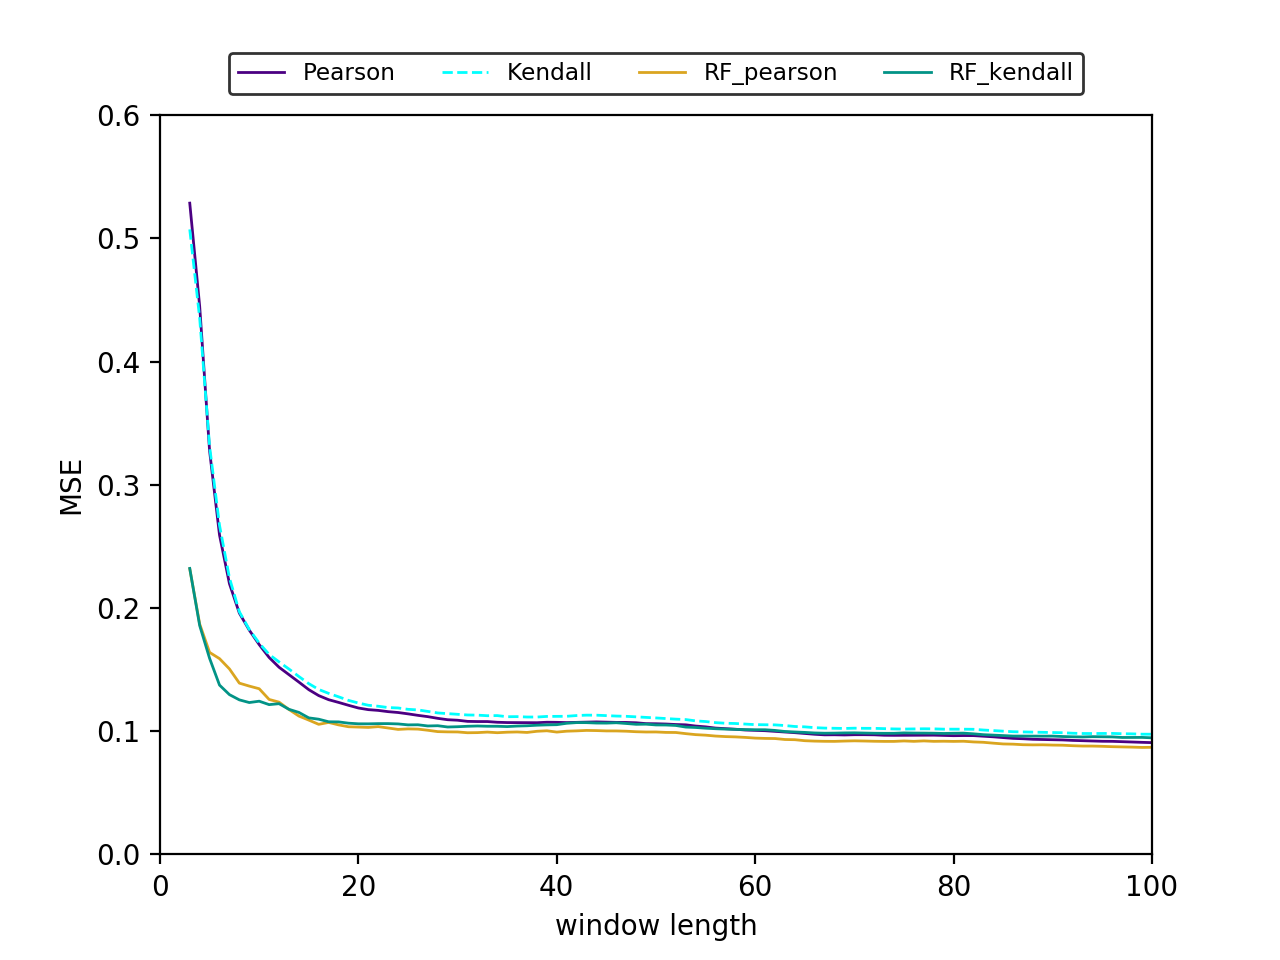
\includegraphics[width=\textwidth, height=0.5\textwidth]{mse_rf10_pearson_kendall_comp_proxy.png}
		%\caption{MSE for RF with covariates from Pearson and Kendall and proxy correlation.}
		%\label{fig:mse_rf10_pearson_kendall_comp_proxy.png}
	\end{subfigure}
	\caption[MSE for RF(10) under proxy correlation, Pearson and Kendall Moving Window bootstrap estimates.]{Comparison MSE for RF(10) with proxy correlation, Pearson and Kendall Moving Window bootstrap estimates.}
	\label{fig:mse_rf10_pearson_kendall_comp_proxy.png}
\end{figure}



\clearpage






\section{Conclusions Simulation Results} \label{sec:conclusions_sim}
In this chapter, using simulation, performance of parsimoniously specified nonparametric k-nearest neighbor (KNN) and random forest (RF) estimators of conditional correlation has been compared against conventional moving windows in terms of the mean squared error (MSE). Conclusions hold for the particular conditional correlation dynamics generated by \eqref{eq:correlation_simulation} but the simulation study provides initial evidence on the general use of KNN and RF as nonparametric estimators of conditional correlation between financial variables. The main conclusions may be summarized as follows: \\

\noindent
First, the conditional correlation matrix obtained from KNN and RF estimators satisfies the condition of positive semidefiniteness. A variety of different parameterizations of both learning estimators has been shown to all yield positive semidefinite conditional correlation matrices, regardless whether the response variable was approximated by Pearson or Kendall sample correlations using moving windows or specified by true correlation.   \\

\noindent
Secondly, default parameterizations, that is, KNN(5) and RF(10) and alternative parameterizations of proposed learning estimators improve over conventional moving window estimates of conditional correlation in terms of lower MSE, especially for smaller window sizes. Moreover, both default and alternative parameterizations of proposed learning estimators improve over conventional moving window estimates of conditional correlation in terms of decreasing the sensitivity to the choice of window length, which is exhibited through significantly lower variance of MSE. Additionally, the uncertainty in the conditional correlation $\rho_t$, which is illustrated by 99\% confidence intervals, is smaller for proposed learning estimators compared to Pearson and Kendall sample correlation estimates using moving windows. Additionally, learning estimates with approximated covariates and response variable follow the increases and decreases of the actual correlation smoother, with tighter confidence intervals. This is a more desirable result as it is not expected that correlation between assets changes that drastically at each time unit.     \\

\noindent
Thirdly, both learning estimators, regardless whether the response variable was approximated by Pearson or Kendall sample correlations or specified by true correlation, exhibit expected behavior under different parameterizations given the theoretical analysis of the decomposition of MSE into squared bias and variance terms; an increase in the number of neighbors in the KNN algorithm or an increase in the number of decision trees in the RF algorithm reduced the variance in both estimators. Of note, an increase in the number of neighbors initially yields a decrease in squared bias. As discussed, a potential explanation may be that inclusion of additional neighbors containing informational value yields more accurate estimates of correlation, that is, a decrease in squared bias. As of some number of additional neighbors, however, only noise is added to the estimation process which results into increased squared bias.      \\


\noindent
In summary, parsimoniously specified KNN and RF estimators improve on predictive capability of conditional correlation compared with Pearson and Kendall sample correlation estimates using moving windows, both in terms of lower MSE and decreasing sensitivity to the choice of window length. Moreover, proposed learning estimators yield positive semidefinite conditional correlation matrices and show expected behavior under different parameterizations in terms of MSE decomposition. Using simulation, initial evidence has been provided on the potential application of proposed learning estimators in high dimensional systems of correlations, which is the topic in Chapter \ref{chap:multivariate_analysis}.   


\iffalse
\begin{enumerate}
	\item KNN with true correlation AND KNN with approximated output return positive semidefinite correlation matrices.
	\item RF with true correlation AND RF with approximated output return positive semidefinite correlation matrices.
	\item The difference in accuracy, measured by the MSE, between using Pearson and Kendall approximations of true correlation appear negligible small for the simulation study, regardless whether Nearest Neighbor or Random Forest algorithm was used.  
	\item KNN with true correlation outperforms moving window estimates particularly for smaller window sizes but with full training set and preferably inverse distance weighting function for all window sizes in the interval [3, 100]. A uniform weighting function results in more or less constant correlation, the very idea we try to improve on by considering correlation to be conditional. This result is also obtained when response variable is approximated. Optimization over hyperparameter $k$ shows that with an increase in $k$ variance is reduced (and bias initially) and correlation estimates become increasingly smooth.
	\item RF with true correlation outperforms, even with default parameterization, moving window estimates for all window sizes sizes in the interval [3, 100]. This shows through lower MSE. In addition, RF is far less sensitive to the choice of window length than moving window estimates, which shows through significantly lower variance of MSE. 
	\item Both KNN and RF estimates with true correlation as response variable are rather volatile for under default parameterizations. With an increase in the number of neighbours and trees, the correlation estimates follow follow the increases and decreases of the actual correlation smoother, with tighter confidence intervals.
	\item MSE decomposition behavior KNN with true correlation exactly as expected  given MSE decomposition formulas. Except that with an increase in $k$, we initially observe improved squared bias. Can be explained by the fact that initially an increase in $k$ results in using more data points with informational value for predicting the response variable. After some $k$, the inclusion of more data points results in incorporating noise in the prediction, and we observe an increase in bias.
	\item MSE decomposition behavior RF with true correlation exactly as expected  given MSE decomposition formulas. An increase in number of trees results into diminishing reduction of variance (and, consequently, a decrease in MSE).
	\item Both KNN and RF estimates with approximated correlation as response variable exhibit lower variance than their parameterizations with true correlation as response variable.
	\item RF exhibits higher bias than KNN. RF thus seems less appropriate model at this point. However, given the very small covariate dimension very little decorrelation of trees is possible which would results in variance reduction and possibly MSE reduction (if bias increase is not too big). Given higher dimensional covariate space in context of systems of correlations we continue to opt for RF estimation of conditional correlations. 
	\item Both KNN and RF estimates with approximated correlation as response variable follow the increases and decreases of the actual correlation smoother, with tighter confidence intervals in comparison to KNN and RF estimates with true correlation as the response variable. This is a more desirable result as it is not expected that correlation between assets changes that drastically at each time unit. 
	\item TAKE ALL THE RESULTS FROM ABOVE AND WE HAVE A MAIN RESULT FROM THE SIMULATION STUDY: parsimonious nearest neighbor and random forest models, where the set of covariates and response variable(s) are constructed from approximation of true correlation using Pearson and Kendall moving window estimates, improve on predictive capability of conditional correlation compared with Pearson and Kendall moving window estimates. Moreover, the resulting conditional correlation matrix $R_t$ satisfy the positive semidefinite criterion. This gives enough reason to extend our problem to higher dimensional dataset constructed from real time series data.   
\end{enumerate}
\fi


%%%%%%%%%%%%%%%%%%%%%%%%%%%%%%%%%%%%%%%%%%%%%%%%%%%%%%%%%%%%%%
%%%%%%%%				      SYSTEMS OF CORRELATIONS							%%%%%%%%%
%%%%%%%%%%%%%%%%%%%%%%%%%%%%%%%%%%%%%%%%%%%%%%%%%%%%%%%%%%%%%%
\chapter{Systems of Correlations in Quantitative Financial Risk Management} \label{chap:multivariate_analysis}
This chapter concerns modeling the dependence structure between financial returns in a multivariate setting. Correlation defined by Pearson's linear coefficient and Kendall's $\tau$ coefficient continue to be the measure for dependency. However, the focus of analysis in a multivariate setting is a \textit{system of correlations} rather than \textit{individual correlations}. The role of systems of correlations is demonstrated in the financial task of risk assessment. \\

\noindent
Value-at-Risk is the mandated measure for downside market risk under regulation of the Basel Accords and estimation of conditional volatility is an essential input for computation of Value-at-Risk in practice. This chapter will illustrate the adequacy of our semiparametric multivariate volatility model in translating the theory of contemporary downside risk assessment into practice for the daily log returns of the 30 constituents included in the Dow Jones Industrial Average index. First, in section \ref{sec:VaR}, notation is established that is necessary to study the risk of portfolios consisting of an arbitrary number of assets. Section \ref{sec:backesting} then describes the backtesting methodology that is applied to statistically compare our semiparametric multivariate volatility model against a parametric counterpart, the dynamic conditional correlation model of \cite{ref:Engle2002}. Next, our semiparametric multivariate volatility model is applied to the 30 constituents included in the Dow Jones Industrial Average index and performance is verified in terms of economic loss functions, the Value-at-Risk and Conditional Value-at-Risk. As such, section \ref{sec:data} contains some descriptive statistics of the dataset comprising log return series of the 30 constituents included in the Dow Jones Industrial Average index and section \ref{sec:results} presents the results. Finally, section \ref{sec:conclusions_emp} concludes the chapter.  \\

\clearpage

\section{Value-at-Risk Theory} \label{sec:VaR}
One definition of Value-at-Risk (VaR) is the maximum loss that is not exceeded at a given confidence level $\alpha$, which is analogous to saying VaR is the loss value for which the probability of observing a larger loss is equal to $1-\alpha$. A more formal definition in terms of the $\alpha$-quantile of the loss distribution is given by \citep{ref:QRM2015}, that is,

\begin{align}
	VaR_{\alpha} = inf\{l \in \mathbb{R}:P(L>l) \le 1-\alpha\}=inf\{l \in \mathbb{R}: F_L(l) \ge \alpha\}
\end{align}

\noindent
where $\alpha \in (0,1)$ and $F_L(l) = P(L \le l)$ denotes the distribution function of the corresponding loss distribution. \\

\noindent
VaR provides a single measure of risk that is easy to understand and has been the mandated measure for downside market risk under regulation of the Basel Accords. However, VaR suffers from several drawbacks for which it has has been heavily criticized by regulators, practitioners and academics alike. One of the foremost criticisms of VaR is that the measure does not provide any insight in or control of losses exceeding VaR; VaR as a risk measure disregards the extreme right tail of the loss distribution, which may be quite an undesirable property exposing one to high uncontrollable risks. Another criticism is that VaR is not a coherent risk measure in case of non-elliptical loss distributions as it lacks the property of subadditivity \citep{ref:Artzner2001}; VaR contradicts the idea that risk can be reduced by diversification. A risk measure that accounts for losses exceeding VaR and remains coherent is the Conditional Value-at-Risk. More formally,   

\begin{align}
	CVaR_{\alpha} = \mathbb{E} [L | L > VaR_{\alpha}]
\end{align}

\noindent
In other words, CVaR is the expected loss given that the loss $L$ exceeds VaR. \\

\noindent
VaR and CVaR are determined after definition of the portfolio return distribution, where portfolio return $p_t = w' r_t$. It is noted that the validation of the portfolio risk using backtesting measures is not straightforward without further assumptions on $a_t$, the distribution of errors driving the volatility process. In this paper, the multivariate Gaussian distribution is considered for the distribution of $a_t$. The first two moments of the conditional portfolio return are given by

\begin{align}
	\mathbb{E}[p_t] &= \mu_{p,t} =  w' \mathbb{E}[\mu_t]  \\
	Var[p_t] &= \sigma_{p,t}^2 =  w'H_tw 
\end{align}

\noindent
If the conditional distribution of each asset return is assumed Gaussian, then the portfolio return also follows a Gaussian distribution as the multivariate Gaussian distribution is closed under linear transformations. In that case, the portfolio return distribution is given by

\begin{align}
	p_t \sim \mathcal{N}(w' \mathbb{E}[\mu_t], w'H_tw)  \nonumber
\end{align}

\noindent 
The portfolio (C)VaR under multivariate normality assumption for one day horizon at $\alpha$ confidence level is then given by

\begin{align}
	VaR_t(\alpha) &= -\mu_{p,t} - \sigma_{p,t} \ \Phi^{-1}(\alpha)  \label{eq:var_parametric_norm} \\
	CVaR_t(\alpha) &= -\mu_{p,t} - \sigma_{p,t} \ \frac{\phi(\Phi^{-1}(\alpha))}{1-\alpha} \label{eq:cvar_parametric_norm}
\end{align}

\noindent 
where $\phi$ denotes the density and $\Phi$ the distribution function of the standard Gaussian distribution. \\

\noindent
The assumption of multivariate normality has been proven inadequate in volatile market conditions where the portfolio return distribution exhibits leptokurtic properties; VaR estimates tend to (severely) underestimate true risk. In order to capture leptokurtic properties, the multivariate Student t distribution is considered for the distribution of $a_t$; the first two moments of the conditional portfolio return is given by    

\begin{align}
	p_t \sim t_v (w' \mathbb{E}[\mu_t], w'H_tw)  \nonumber
\end{align}

\noindent 
The portfolio (C)VaR under multivariate Studen t assumption for one day horizon at $\alpha$ confidence level is then given by 

\begin{align}
	VaR_t(\alpha) &= -\mu_{p,t} - \sigma_{p,t} \ \sqrt{\frac{v-2}{v}} \ t_v^{-1}(\alpha) \label{eq:var_parametric_std} \\
	CVaR_t(\alpha) &= -\mu_{p,t} - \sigma_{p,t} \ \sqrt{\frac{v-2}{v}} \ \frac{g_v(t_v^{-1}(\alpha))}{1-\alpha} \ \Big(\frac{v+(t_v^{-1} (\alpha))^2}{v-1} \label{eq:cvar_parametric_std}\Big)
\end{align}

\noindent
where $g_v$ denotes the density and $t_v$ the distribution function of the standard Student t distribution. \\

\noindent
In the backtesting analysis, VaR is computed at different quantiles of the loss distribution in order to compare performance of different risk models across the entire distribution of results. In contrast, CVaR is only computed at the 0.99 quantile of the loss distribution as this is the VaR quantile on which the calculation of capital requirement for market risk is premised in practice. For simplicity, but without loss of generality, the unconditional mean is used as the conditional mean filtration given that the dynamic dependence in the conditional means of portfolio returns are generally weak and not significantly affecting VaR results. The VaR for a long position in an equally weighted portfolio is considered as a number of papers \citep{ref:Plyakha2012} suggest that equally weighted portfolio strategies consistently outperform other optimization strategies. Moreover, the focus in this part of the analysis is on the empirical evaluation of different models for modeling and forecasting of the conditional covariance matrix instead of finding optimal portfolio weights or any form of risk minimization.    \\


\iffalse
\subsection{High Density Regions}
\textbf{ALTERNATIVE COMPUTATION OF VAR: Highest Density Regions.}\\
Alternatively, for obtaining VaR (quantiles) from a multivariate normal distribution we can report VaR as the multivariate  'sample quantiles', leading to highest density regions. \\

\noindent
Highest density regions are well suited for the purpose of forecast accuracy evaluation. One of the most distinctive property of HDR's is that of all possible regions of probability coverage $1-\alpha$, the HDR has the smallest region possible in the sample space. In the one-dimensional continuous case that would be the shortest interval, and in the two-dimensional case that would be the smallest area of the surface.   


\begin{itemize}
	\item Highest density region (HDR) ($\alpha$) is defined as the area with the smallest interval that spans $1-\alpha$ of the density.
	\item The region covering the sample space for a given probability $1-\alpha$, should have the smallest possible volume.
	\item Every point inside the region should have probability density at least as large as every point outside the region.
	\item  In the case of a normal distribution an HDR coincides with the usual probability region symmetric about the mean, spanning the a/2 and 1 - a/2 quantiles. 
	\item It follows that the number of disjoint intervals in a highest density region can never exceed the number of modal groups in the density function. 
	\item The inverse cdf of a normal corresponds to the quantile function of a normal.
	\item As long as you can define a function that evaluates the CDF, you can find quantiles. 
	\item  One major problem is the computational  difficulty in numerically integrating over a general region in  high-dimensional space. An alternative approach is required that avoids explicit integration:
\end{itemize}

\noindent
"Although the reduced models, in which the portfolio's returns are considered as one single univariate time series, can be used to calculate VaR for large portfolio, the reduced models (univariate method) may yield low accuracy by ignoring the complicated correlation among the individual returns. Consequently, reduced models provide less detailed information on the source of risk. \iffalse https://pdfs.semanticscholar.org/13c3/84e1928796f06618f812262836c64664db6e.pdf \fi
Problematic: extension of VaR to the multivariate framework is not unique because a unique definition of multivariate quantile does not exist."
\fi

\clearpage

\section{Backtesting Methodology} \label{sec:backesting}
Backtesting is the process of verifying whether one's model performs adequately. In this paper, the goal of a backtesting procedure is to statistically evaluate proposed semiparametric multivariate volatility model against the DCC model of \cite{ref:Engle2002} and potentially detect any misspecification of the risk model. \cite{ref:Christoffersen1998} defined two properties that must both be satisfied by a valid VaR model: unconditional coverage property and independence property. Two statistical tests are considered in this paper for the assessment of these two properties: a failure test of unconditional coverage using the Kupiec test \citep{ref:Kupiec1995} and an independence test using Christoffersen's Markov test \citep{ref:Christoffersen1998}. All test results are provided at the 5\% significance level. \\

\noindent
\cite{ref:Kupiec1995} developed a statistical test to asses the unconditional coverage of a VaR model; the hypothesis that the the total number of exceedances equals the expected number of exceedances, given the independence property is satisfied. \cite{ref:Kupiec1995} tests for unconditional coverage through formulation of a log-likelihood ratio, that is,

\begin{align} \label{eq:Kupiec_test}
	LR_{uc} = 2 \ \text{ln} \Bigg( \bigg(\frac{1-I(\alpha) / T}{1-\alpha}\bigg)^{T-I(\alpha)} \bigg(\frac{I(\alpha) / T}{\alpha} \bigg)^{I(\alpha)}\Bigg)
\end{align}

\noindent
In \eqref{eq:Kupiec_test}, $T$ is the number of observations and $I(\alpha)$ is the total number of exceedances. An exceedance $I_t(\alpha)$ is defined as $r_{t+1} < VaR_t(\alpha)$. The test statistic is asymptotically distributed as a chi-square distribution with 1 degree of freedom under the null hypothesis that the VaR model is adequate, that is, the VaR model produces an expected proportion of exceedances equal to $\alpha$. Moreover, as the Kupiec test statistic is two sided, the model under consideration is rejected in the following two cases: there are too few exceedances, which implies the model is excessively conservative, or there are too many exceedances, that is, an underestimation of risk.   \\

\noindent
An important shortcoming of Kupiec's test is that it solely examines the frequency of exceedances but neglects to assess any form of independence in the occurrence of exceedances. As a consequence, the test may fail to reject a model producing clustered VaR exceedances. This is problematic because, in theory, one would expect exceedances to be evenly spread over time. A clustering of exceedances implies the independence property is violated as an adequate VaR model should exhibit responsiveness to changing market conditions, such as changes in volatility and correlations, thereby making clustered exceedances less likely. Exceedance clustering is an important concept as consecutive unexpected losses may be more stressful to an institution compared to unexpected losses occurring somewhat more frequently than expected but are evenly spread out over time  \citep{ref:Campbell2005}. Christoffersen's Markov test \citep{ref:Christoffersen1998} is one of a variety of tests that explicitly examines the independency property of VaR exceedances. The Markov test examines whether the likelihood of a VaR exceedance depends on whether a VaR exceedance occurred on the previous day. Under the null hypothesis, the probability of an exceedance proceeded by a non-exceedance equals the probability of an exceedance proceeded by an exceedance, that is, $\pi_{01} = \pi_{11}$ in \eqref{eq:Christoffersen_test}. In other words, the probability of exceeding today's VaR should be independent of whether yesterday's VaR was exceeded or not. Only then the VaR measure accurately reflects the underlying portfolio risk \citep{ref:Campbell2005}. \cite{ref:Christoffersen1998} observed that testing for independence can be formulated as a log-likelihood ratio test, that is, 

\begin{align} \label{eq:Christoffersen_test}
	LR_{ind} = -2 \ \text{ln} \Bigg(\frac{(1-\pi_2)^{(n_{00}+n_{10})}\pi_2^{(n_{01}+n_{11})}}{(1-\pi_{01})^{n_{00}}\pi_{01}^{n_{01}}(1-\pi_{11})^{n_{10}}\pi_{11}{^{n_{11}}}} \Bigg)
\end{align}

\noindent
where $n_{ij}$ is the number of transitions from $i$ to $j$ in the hit sequence function $I_t$, with $i,j \in \{0,1\}$, corresponding to non-exceedances and exceedances. The transition probability $\pi_{ij} = n_{ij} / \sum_j n_{ij}$ and $\pi_2 = (n_{01}+n_{11}) / (n_{00}+n_{10}+n_{01}+n_{11})$. Moreover, the test statistic is asymptotically distributed as a chi-square distribution with 1 degree of freedom under assumption of the null hypothesis. \\

\noindent
The main assumption underlying Christoffersen's Markov test is that the hit sequence function of exceedances and non-exceedances satisfies the Markov property. However, \cite{ref:Christoffersen1998} only considers first order dependence, through a first-order Markov chain model, and this is considered a weakness of the independence test.   \\

\noindent
Furthermore, we are interested in how adequate the risk models capture losses exceeding VaR, that is, the CVaR. We follow \cite{ref:McNeil2000} and define the exceedance residual series as

\begin{align}
	\text{er}_t(\alpha) &= L_t - \text{CVaR}_t(\alpha) \ \text{I}_t \{L_t < \text{VaR}_t(\alpha) \}  \label{eq:cvar_er}
\end{align}  

\noindent
where $L_t$ is actual portfolio loss on day $t$ and $\text{I}_t\{L_t < \text{VaR}_t(\alpha) \}$ is the indicator function taking on the value 1 if the portfolio loss on day $t$ exceedes VaR at day $t$ and 0 otherwise.  \\

\noindent
The minimum exceedance residual, min($er_t$), and mean exceedance residual, mean($er_t$), are reported. If the minimum exceedance residual number is negative, then that indicates the CVaR$_t$ was exceeded at least once, that is, the actual loss $L_t$ was greater than CVaR$_t$ for some $t$ in the backtest period. This means that CVaR was underestimated for at least one occasion. If the minimum exceedance residual returns a positive number, then that indicates that CVaR$_t$ was never exceeded given VaR$_t$ was exceeded for all $t$ in the backtest period. Moreover, a positive value for min($er_t$) implies that the risk model overestimates CVaR throughout the entire backtest period. The mean exceedance residual sign and magnitude give us information whether CVaR is, on average, under- or overestimated and to what extend, respectively. In general, a risk manager would prefer a risk model where the estimated CVaR deviates as little as possible from the actual portfolio loss. Underestimation of true risk by risk models may result into excessive capital allocated to risky positions, which may result in greater losses than expected and, consequently, decreased profits. Similarly, overestimation of true risk by risk models may result into excessive capital reserves, which also decrease profits. In any case, a risk model where $|$min($er_t$)$|$ and $|$mean($er_t$)$|$ are smaller compared with alternative risk models is preferred.     


\section{Data and Descriptive Statistics} \label{sec:data}
The dataset comprises 30 univariate time series of the log returns included in the Dow Jones Industrial Average index (DJIA). The return series cover data from March 1987 to December 2001 and originate from Yahoo Finance. During this period, financial markets experienced tranquil periods with low volatility such as the mid-1990's as well as periods of high volatility including the collapse of the Dot-com bubble. Figure \ref{fig:DJIA_returns} shows the daily mean log return series of the DJIA constituents. The extreme large loss in 1987 correspond to "Black Monday", the world wide stock market crash of October 19, 1987. After a relative tranquil period during the mid 1990's a period of high volatility followed with the collapse of the Dot-com bubble in the spring of 2000 and the collapse of Enron and WorldCom companies. The large loss incurred in 2001 corresponds to he September 11 attacks of 2001. By visual inspection, the heteroskedastic behavior of the return series becomes apparent, indicating volatility clustering, and provides evidence for specifying a model for the conditional variances to capture this behavior.        

\begin{figure}[H]
	\centering
	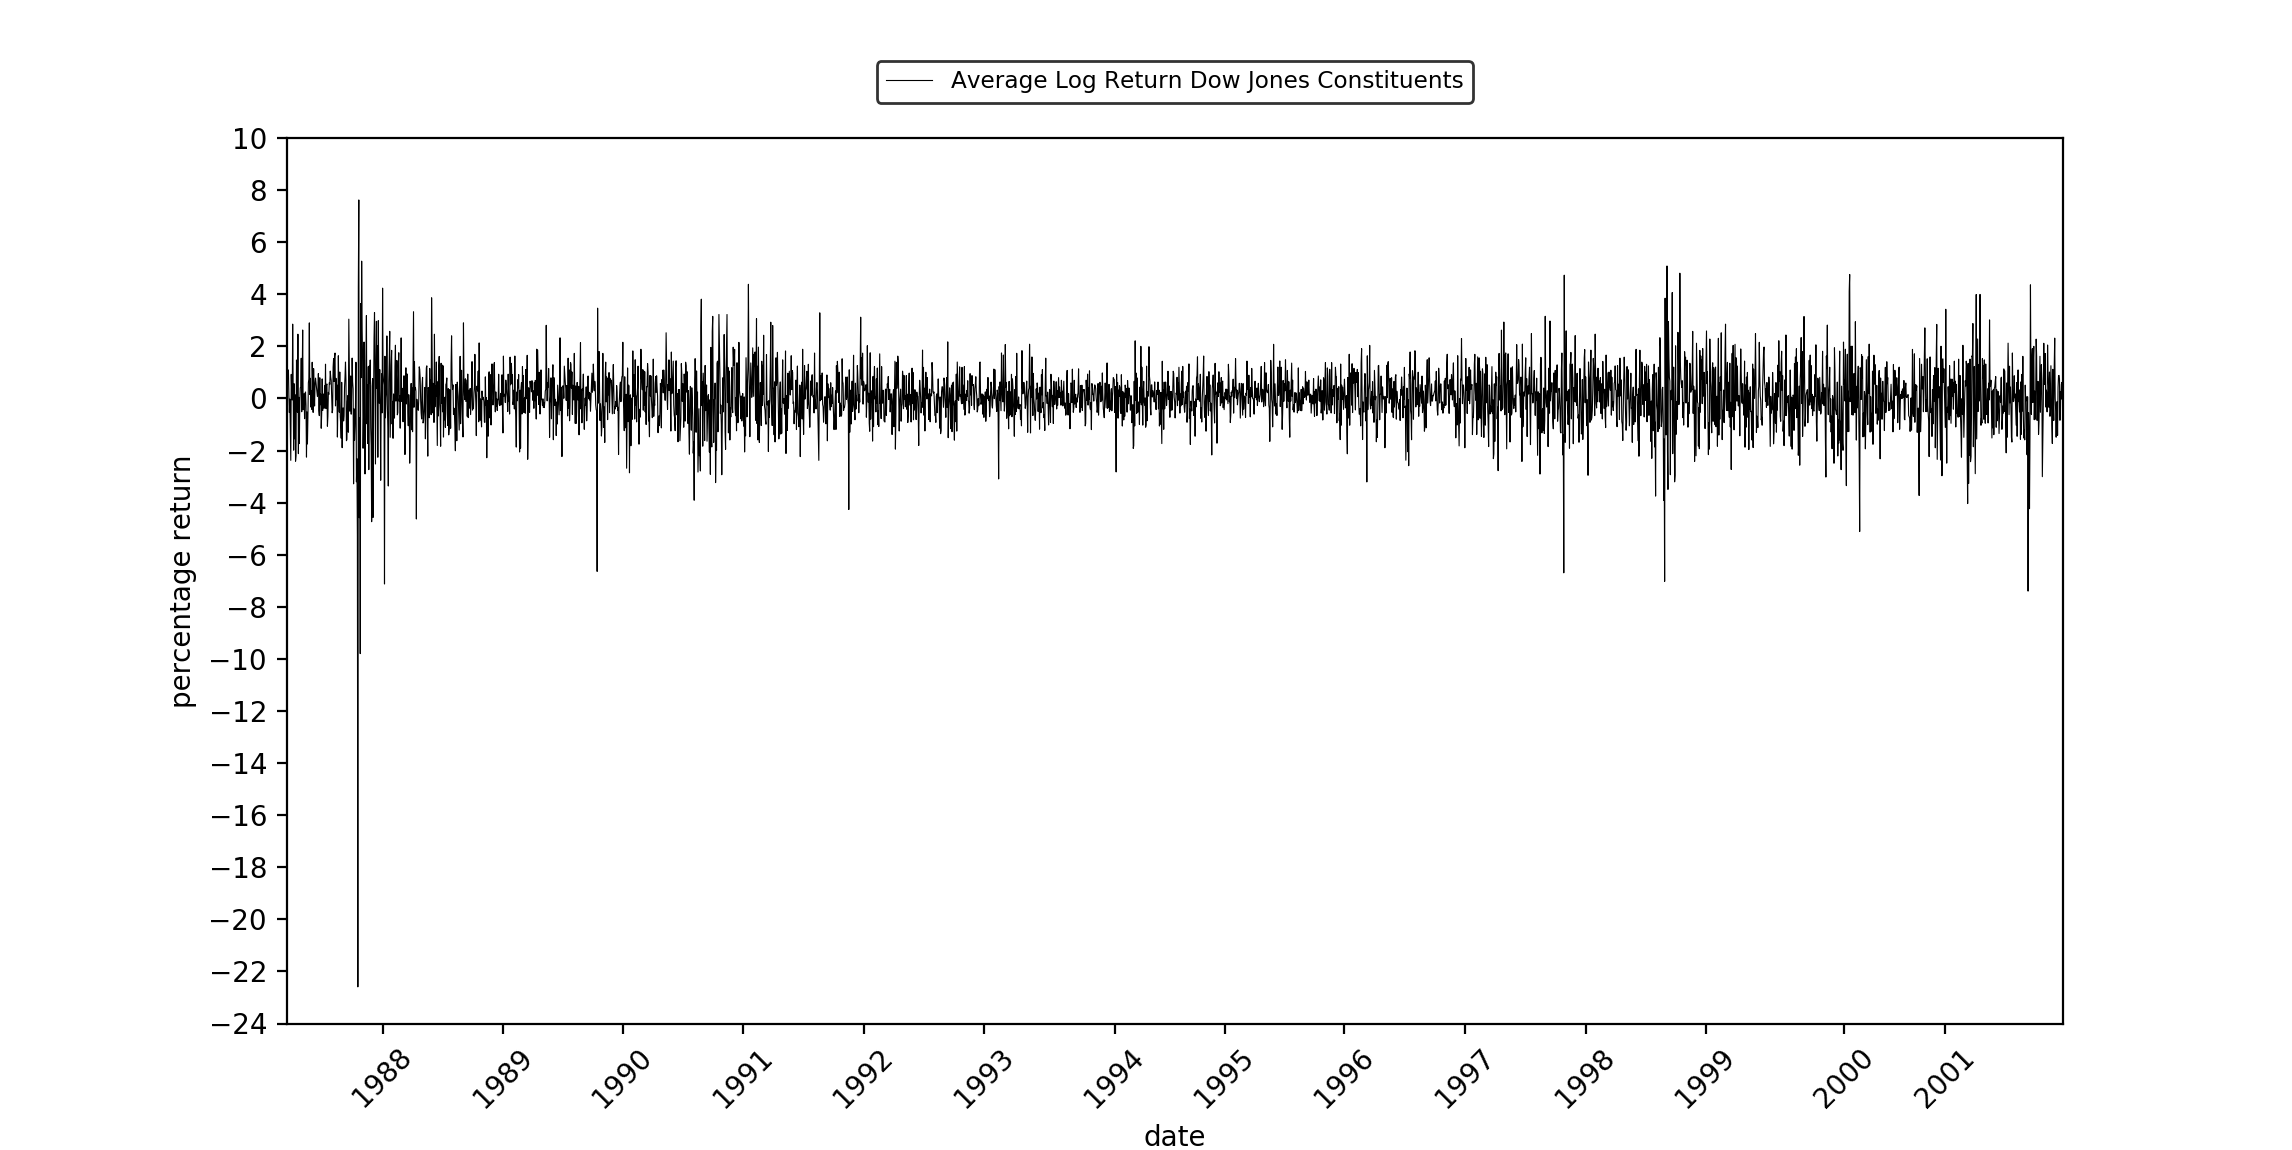
\includegraphics[scale=0.6]{multivar_analysis/log_returns_DJ_constituents.png}
	\caption{Log return of a long position in an equally weighted portfolio comprising the 30 Dow Jones Industrial Average constituents from March 1987 to December 2001.}
	\label{fig:DJIA_returns}
\end{figure}

\subsection{Summary Statistics}
Tabel \ref{tab:stats_data} presents summary statistics on the 30 marginal time series of the log returns included in the DJIA. Of particular note is the negative skewness of the return series and the excess kurtosis for all 30 assets. \iffalse www.tandfonline.com/doi/pdf/10.1080/07350015.2016.1177535?needAccess=true \fi All asset return series exhibit an excess kurtosis indicating a higher probability of large negative and positive returns than would be expected under normality. Additionally, all return series exhibit negative skewness which indicates more frequent large negative returns than large positive returns. In other words, all series exhibit behavior that departs from normality. The departures from normality are verified with a Jarque-Bera test \citep{ref:Jarque1980} under the null hypothesis that the sample is drawn from a distribution with a skewness and excess kurtosis equal to that of the normal distribution, that is, skewness and excess kurtosis are zero. The Jarque-Bera test rejects the assumption of normality for all assets. This motivates considering specifications for the conditional variance and marginal error distributions in order to capture the exhibited excess kurtosis and skewness. 



\subsection{Conditional Variance Model}
As discussed in Section \ref{sec:VaR}, for simplicity, but without loss of generality, the conditional mean of our data is specified by the unconditional mean. Our model for the conditional variance is the GARCH(1,1) model of \cite{ref:Bollerslev1986} with the marginal distributions of the standardized residuals specified as the standard Gaussian distribution. Additionally, we consider the asymmetric volatility model of \cite{ref:Glosten1993}, the Glosten-Jagannathan-Runkle-GARCH (GJR-GARCH) model, as specification for the conditional variance. The choice for the asymmetry in this model is motivated by the asymmetric response of volatility to positive and negative asset returns; a asymmetric negative correlation between asset return change and volatility change implies that the rise in volatility following negative returns is generally larger than the fall in volatility following positive returns. The GJR-GARCH(1,1) model accounts for this inverse relationship between first and second order moments of asset returns, that is,

\begin{align} \label{eq:gjr_garch}
	\sigma^2_{i,t} = \omega_i + \beta_i \sigma^2_{i,t-1} + \alpha_i a^2_{i,t-1} + \gamma_i a^2_{i,t-1} I_{t-1}\{a_{i,t-1} < 0 \} 
\end{align}

\noindent
For the marginal distributions of the standardized residuals from GJR-GARCH specification we consider the standard skewed Student's t-distribution of \cite{ref:Fernandez1998}, which accounts for nonzero skewness and excess kurtosis, that is, 

\begin{align}
	\eta_{i,t} = \frac{z_{i,t}}{\sigma_{i,t}} \sim \ Skew \ t (0, 1, v_i, \psi_i)  \nonumber
\end{align}


\noindent
Table \ref{tab:stat_dist_gjr_sstd_table} summarizes the results of estimating the GJR-GARCH(1,1) model from \eqref{eq:gjr_garch} on the daily log returns of the 30 constituents included in the DJAI for the initial in-sample period of the volatile market test period (March 1987 to December 1999) for 3235 observations. A Ljung-Box test \citep{ref:Ljung1978} exhibits significant autocorrelation in 15 out of 30 of the daily log returns. For the purpose of verifying the adequacy of the conditional variance and marginal distribution specifications, an ARMA(3,1) model was used to capture autocorrelation remaining in the residual series. The conditional variance models display only moderate statistical indication of asymmetry in volatility given that the estimated asymmetry coefficient, $\gamma_i$, is found statistically significant for only 8 out of 30 assets. However, the sign bias test statistics on the residuals are insignificant for 7 out of 8 of the asymmetric models implying asymmetric response of volatility to positive and negative asset returns is adequately captured by the asymmetric GJR-GARCH model. Moreover, for 6 out of these 7 the effect of positive asset returns are stronger than negative asset returns on future volatility. The average estimated degrees of freedom of the shape parameter is 6.9 and the estimated skewness parameter is positive for all 30 assets, and both estimated parameters are significantly different from zero for all 30 assets, indicating heavy tails and positive skewness.    

\begin{table}[H]
\centering
\captionsetup[subtable]{position=below}
\begin{tabular}{l c c c c c c c}
\toprule
\multirow{2}{*}{}      & \multicolumn{7}{c}{Cross-sectional distribution}                                        \\ \cmidrule{3-8} 
                    &   & Mean       & 5\%       & 25\%      & Median    & 75\%               & 95\%              \\ \midrule 
$\omega_i$         &        & 0.0965     & 0.0211    & 0.0384    & 0.0713    & 0.1023             & 0.2856            \\
$\alpha_i$           &       & 0.0355     & 0.0123    & 0.0281    & 0.0359    & 0.0404             & 0.0600            \\
$\beta_i$             &     & 0.9208     & 0.8840    & 0.9036    & 0.9279    & 0.9416             & 0.9650            \\
$\gamma_i$        &          & 0.0357     & 0.0009    & 0.0135    & 0.0377    & 0.0580             & 0.0734            \\
$v_i$                  &   & 6.9225     & 4.7454    & 6.2507    & 7.0366    & 7.7493             & 8.4095            \\
$\psi_i$               &     & 1.0406     & 1.0043    & 1.0247    & 1.0390    & 1.0529             & 1.0830            \\
\multicolumn{6}{l}{}                                                    & \multicolumn{2}{l}{No. of  Rejections} \\
\multicolumn{6}{l}{LB test for standardized residuals}                  & \multicolumn{2}{c}{2}                  \\
\multicolumn{6}{l}{WP test for squared standardized residuals} & \multicolumn{2}{c}{2}                  \\
\multicolumn{6}{l}{KS test for skew t dist standardized residuals}      & \multicolumn{2}{c}{1}     \\ [1ex]            
\bottomrule  
\end{tabular}
\caption[Summary statistics of GJR-GARCH skewed Student's t model specification for the conditional variance in volatile market conditions.]{Summary statistics of GJR-GARCH(1,1) skewed Student's t model specification for the conditional variance in the initial in-sample period of the volatile market period.} 
\label{tab:stat_dist_gjr_sstd_table}
\end{table}

\noindent
We conclude our discussion on the GJR-GARCH(1,1) model with skewed Student's t-distributed marginals summarizing goodness-of-fit tests for the marginal distribution specification. Table \ref{tab:stat_dist_gjr_sstd_table} shows that a Ljung-Box test for autocorrelation up to the tenth lag rejects the null hypothesis of zero autocorrelation (at the 0.05  significance level) for only two of the standardized residual series. More importantly, the weighted portmanteau test \citep{ref:Fisher2012} rejects the null hypothesis of zero autocorrelation (at the 0.05 significance level) up to the tenth lag for only two of the squared standardized residual series. From the latter one can conclude that the GJR-GARCH(1,1) model provides a satisfactory fit to the conditional volatilities. Next, the null hypothesis  of correct specification of the skewed Student's t-distribution for the standardized residuals is rejected for 1 of the 30 asset return series with a Kolmogorov-Smirnov test using 100 simulations. Table \ref{tab:stat_dist_garch_norm_table} summarizes the results of the estimated ARMA(3,1)-GARCH(1,1) model with a Gaussian specification for the standardized residual series. The table provides strong statistical evidence on misspecification of the Gaussian distribution for the marginal distributions of the standardized residuals as the null hypothesis of correct specification of the Gaussian distribution for the standardized residuals is rejected for all asset return series with a Kolmogorov-Smirnov test using 100 simulations. \\

\noindent
In summary, we can conclude that the GJR-GARCH(1,1) model with standard skewed Student's t-distribution specification for the marginal errors provides an adequate alternative conditional variance model that is capable of capturing the excess kurtosis and skewness exhibited by the daily log returns of the 30 DJIA constituents in our empirical application. This holds for the initial in-sample period of the volatile market test period (March 1987 to December 1999) but similar conclusions hold for the initial in-sample period of the tranquil market test period (March 1987 to December 1993) as supported by tabel \ref{tab:stat_dist_gjr_sstd_tranquil_table} and tabel \ref{tab:stat_dist_garch_norm_tranquil_table}.  

\clearpage

\section{Empirical Results} \label{sec:results}
Model adequacy is verified in tranquil market conditions (mid-1990's) and volatile market conditions (the Dot-com bubble) by considering the following backtest periods; (1) an out-of-sample period from January 1994 to December 1995 for 504 observations corresponding to tranquil market conditions with an initial in-sample period from March 1987 tot December 1993 for 1720 observations; (2) an out-of-sample period from January 2000 to December 2001 for 500 observations corresponding to volatile market conditions with an initial in-sample period from March 1987 to December 1999 for 3235 observations. One-step-ahead out-of-sample forecasts are obtained for the entire out-of-sample period. Conditional volatility and conditional correlation model parameters are re-estimated with the most recent information available, that is, conditional on the information available at time $t-1$. \\

\noindent  
As such, our empirical application proceeds as follows. Using daily log returns of the 30 constituents included in the Dow Jones Industrial Average index for the in-sample estimation period, we 


\begin{enumerate}
	\item Estimate conditional volatility models for each asset.
	\item Use estimates of conditional volatility models to form one-step-ahead conditional volatility forecasts for each asset. 
	\item  Estimate nonparametric conditional correlation models.
	\item Use estimates of conditional correlation model to form one-step-ahead pairwise correlation forecasts.
	\item Combine conditional correlation forecasts with conditional volatility forecasts to construct the conditional covariance matrix forecast according to \eqref{eq:covariance_decomposition}.
	\item Use the conditional covariance matrix forecast to obtain (Conditional) Value-at-Risk forecasts according to \eqref{eq:var_parametric_norm}-\eqref{eq:cvar_parametric_std}.
	\item Backtest (Conditional) Value-at-Risk forecasts according to \eqref{eq:Kupiec_test}-\eqref{eq:cvar_er}.
\end{enumerate} 

\noindent
To recall, there are two different classes of risk models evaluated: first, a fully parametric benchmark is applied to the returns data, the dynamic conditional correlation (DCC) model of \citep{ref:Engle2002}, which is restrictive in that it only considers Gaussian marginals and imposes a functional form on the conditional correlation matrix. The second class consists of our semiparametric multivariate volatility model where conditional correlations are estimated using nonparametric k-nearest neighbor (KNN) and random forest (RF) estimators. With respect to notation: recall that KNN(5)-Pearson-Garch is a semiparametric multivariate volatility model specification where conditional variances are estimated using GARCH(1,1) with standard Gaussian distributed marginals and a k-nearest neighbor estimator with 5 neighbors and Pearson approximations for true correlation is used for estimation of conditional correlations. Analogously, RF(100)-Kendall-GJR is a semiparametric multivariate volatility model specification where conditional variances are estimated using GJR-GARCH(1,1) model with standard skewed student t distributed marginals and a random forest estimator with 100 decision trees and Kendall approximations for true correlation is used for estimation of conditional correlations     \\

\noindent
We will focus our discussion of the VaR backtesting results on the higher quantiles of the portfolio loss distribution, the confidence levels 95\%, 97.5\% and 99\%, as these are most used in practice. Results on the lower quantiles are however presented in appendix \ref{ap:var} and will enter our discussion when commenting on the 95\% VaR results. Forecasting performance on the lower quantiles (less than 95\%) of the portfolio loss distribution is theoretically relevant to evaluate the fitting/forecasting of the risk models; it allows us to explore the distribution of results. Lastly, the different specifications for the conditional variance model, GARCH and GJR, show very little differences in their VaR estimates (GJR estimates tend to be a little bit smoother); thus, only the semiparametric models with GARCH specification for the conditional variance are shown in the figures of sections \ref{sec:tranquil} and \ref{sec:volatile}.  \\

\subsection{Tranquil Market Conditions: Mid-1990's} \label{sec:tranquil}
Table \ref{tab:var_backtest_tranquil_table} presents an overview of the VaR and CVaR backtest results in tranquil market conditions for a long position in an equally weighted portfolio comprising the 30 constituents of the DJIA. The backtest results exhibit some general patterns for all three VaR confidence levels considered; (1) semiparametric multivariate volatility models show less conservative behavior compared with the DCC model; (2) semiparametric multivariate volatility models with Kendall approximations of true correlation exhibit a higher number of VaR exceedances than their Pearson counterpart; (3) semiparametric multivariate volatility models premised on GJR-GARCH specification with skewed student t distributed errors for the conditional volatility exhibit a higher number of VaR exceedances than their GARCH counterpart; (4) the likelihood of a VaR exceedance does not depend greatly on whether a VaR exceedance occurred on the previous day. \\
  
\noindent  
The backtest results indicate that all models except the KNN(5)-Kendall-GJR model are adequate at estimating the 99\% VaR; the null hypothesis of the unconditional coverage and independence test are not rejected at the 5\% significance level. For the 99\% VaR, the DCC and KNN(idw)-Pearson exhibit 2 exceedances whereas the other semiparametric risk models exhibit 3 to 10 exceedances against an expectation of 5.4 exceedances. The KNN(idw)-Kendall model appears to be the most adequate risk model for the 99\% VaR with 6 exceedances, closely followed by the RF(10)-Pearson-GJR and RF(100)-Pearson-GJR risk models with 4 exceedances and the KNN(100)-Kendall risk models with 7 exceedances. \\

\noindent
The backtest results indicate that all models except the KNN(idw)-Pearson-Garch model are adequate at estimating the 97.5\% VaR; the null hypothesis of the unconditional coverage and independence test are not rejected at the 5\% significance level. For the 97.5\% VaR, the DCC and KNN(idw)-Pearson-Garch exhibit 7 exceedances whereas the other semiparametric risk models range from 9 (RF(100)-Pearson-Garch) to 17 (KNN(5)-Kendall-GJR) exceedances whereas 12.6 VaR exceedances are expected. The KNN(5)-Pearson-GJR model appears to be the most adequate risk model for the 97.5\% VaR with 13 exceedances, closely followed by the KNN(100)-Kendall, RF(10)-Kendall and RF(100)-Kendall risk models with 12 exceedances. \\

\noindent
The final VaR considered is the 95\% VaR with 25.2 expected exceedances. The backtest results differ slightly from the 97.5\% and 99\% VaR backtest results. This time, the null hypothesis of the unconditional coverage test is rejected for the DCC, KNN(idw) and RF(100)-Pearson models because they overestimate the true risk considerably with 11 to 13 exceedances. Moreover, tabel \ref{tab:var_backtest_tranquil_table_lower} indicates that the null hypothesis of the unconditional coverage test is rejected for DCC on all lower quantiles except the 0.4 quantile whereas we obtain mixed results on the lower quantiles for KNN(idw) and RF(100). In contrast, KNN(5), KNN(100)-Kendall, RF(10) and RF(100)-Kendall report a number of VaR exceedances between 17 and 27 and the null hypothesis of the unconditional coverage test is not rejected at the 5\% significance level. Moreover, tabel \ref{tab:var_backtest_tranquil_table_lower} indicates that the null hypothesis of the unconditional coverage and independence test is not rejected at the 5\% significance level for the KNN(100)-Kendall risk model across the entire loss distribution. In other words, we have an indication that KNN(100)-Kendall is an adequate risk model across more than only the higher quantiles of the loss distribution in terms of estimating VaR in tranquil market conditions. The KNN(5)-Pearson-GJR model is the only model that rejects the null hypothesis of the independence test at the 5\% significance level implying estimated VaR exceedances are not independently distributed in this risk model. The KNN(5)-Kendall-Garch model appears to be the most adequate risk model for the 95\% VaR with 25 exceedances, closely followed by the KNN(5)-Kendall-GJR risk model with 27 exceedances. The KNN(100)-Kendall model is a bit conservative for the 95\% VaR but remains adequate across the considered loss distribution. \\

\noindent
The minimum exceedance residual, min($er_t$), for the 99\% VaR is negative for all risk models. This implies that no risk model under consideration ensures that CVaR is never exceeded in the backtest period. Similarly, the mean exceedance residual, mean($er_t$), is also negative for all risk models. This implies that, on average, all risk models under consideration tend to underestimate true CVaR, that is, they tend to underestimate, on average, the actual portfolio loss $L_t$ given that the loss $L_t$ exceeds VaR$_t$. In terms of min($er_t$) and mean($er_t$), the KNN(idw)-Pearson-Garch model and KNN(100)-Kendall-Garch model, respectively, deem the most adequate risk models for the 99\% CVaR.   \\
    
\begin{landscape}
\pagestyle{empty}
\begin{table}[h]
\centering
\captionsetup[subtable]{position=below} 
\begin{tabular}{l c c c l l l l l l c c}
\toprule
\multicolumn{1}{c}{{\underline{Model}}} & \multicolumn{3}{c}{{\underline{VaR Exceedances}}} & \multicolumn{6}{c}{{\underline{VaR Transition Probabilities}}} &  \multicolumn{2}{c}{{\underline{CVaR Exceedance Residuals}}}                                                                         \\
                                & I(0.95)  & I(0.975)  & I(0.99) &  \multicolumn{2}{c}{I(0.95)} & \multicolumn{2}{c}{I(0.975)} & \multicolumn{2}{c}{I(0.99)}   & \multicolumn{2}{c}{I(0.99)}\\ \cmidrule{2-12} 
                                &          &                   &                  & \multicolumn{1}{c}{{$\pi_{01}$}}       & \multicolumn{1}{c}{{$\pi_{11}$}}       & \multicolumn{1}{c}{{$\pi_{01}$}}        & \multicolumn{1}{c}{{$\pi_{11}$}}       & \multicolumn{1}{c}{{$\pi_{01}$}}       & \multicolumn{1}{c}{{$\pi_{11}$}} & \multicolumn{1}{r}{min($er_t$)}  & \multicolumn{1}{c}{{mean($er_t$)}}    \\  \midrule 

DCC-Garch				&\textbf{11}	&7	&2              &0.0203              &0.0909              &0.0121               &0.1429              &0.004             &0  &-0.5206  & -0.2143    \\
DCC-GJR		  			&\textbf{11}	&7	&2         &0.0203      &0.0909       &0.0121       &0.1429         &0.004              &0   &-0.5003	&-0.1786          \\  \midrule 
KNN(5)-Pearson-Garch            	&17          &11           &7                        &0.0309              &0.1176              &0.0203               & 0.0909             &0.0121              &0.1429    &-0.4387	&-0.1250          \\
KNN(5)-Pearson-GJR              	&19		&13		&7         	&\textbf{0.0331}	&\textbf{0.1579}	&0.0245           &0.0769              &0.0121              &0.1429   &-0.4978	&-0.1672           \\
KNN(5)-Kendall-Garch            	&25	&15	&10                       &0.046              &0.12              &0.0287               &0.0667              &0.0183              &0.1   &-0.7269	&-0.1678           \\
KNN(5)-Kendall-GJR              	&27		&17		&\textbf{11}                   &0.0504              &0.1111              &0.0309               &0.1176              &0.0203              &0.0909    &-0.7666	&-0.1687          \\
KNN(100)-Kendall-Garch          &17		&12		&7                     &0.0329              &0.0588              &0.0224               &0.0833              &0.0121              &0.1429     &-0.5830	&-0.0363$^{*}$         \\
KNN(100)-Kendall-GJR             &18		&12		&7                     &0.0330              &0.1111              &0.0224               &0.0833              &0.0121              &0.1429      &-0.6167	&-0.0671        \\
KNN(idw)-Pearson-Garch          &\textbf{11}	&\textbf{6}		&2                     &0.0203              &0.0909              &0.0121               &0              &0.004              &0     &-0.4094$^{*}$		&-0.1586         \\
KNN(idw)-Pearson-GJR         	&\textbf{11}	&7	&2                   &0.0203             &0.0909              &0.0121               &0.1429              &0.004              &0     &-0.4421	&-0.1952         \\
KNN(idw)-Kendall-Garch          	&\textbf{12}	&10	&6                      &0.0224              &0.0833              &0.0183               &0.1              &0.0121             &0        &-0.7752		&-0.0438      \\
KNN(idw)-Kendall-GJR          	&\textbf{13}	&11	&6                     &0.0245             &0.0769              &0.0203               &0.0909              &0.0121            &0      &-0.8023	&-0.0756        \\  \midrule 
RF(10)-Pearson-Garch            	&17		&10		&3                      &0.0309              &0.1176             &0.0183               &0.1              &0.006              &0      &-0.5745	&-0.2085        \\
RF(10)-Pearson-GJR             	&17		&11		&4                    &0.0309             &0.1176              &0.0203               &0.0909              &0.008              &0     &-0.6000	&-0.1256         \\
RF(10)-Kendall-Garch            	&18	&12	&8        &0.0803                           &0.0556              &0.0224               &0.0833              &0.0141              &0.125    &-0.8648	&-0.0957         \\
RF(10)-Kendall-GJR              	&21		&12		&10	                       &0.0415              &0.0476              &0.0224               &0.0833              &0.0183              &0.1         &-0.8880	&-0.0595     \\
RF(100)-Pearson-Garch           	&\textbf{11}	&9	&3                       &0.0203              &0.0909              &0.0162               &0.1111              &0.006              &0       &-0.5019	&-0.1783       \\
RF(100)-Pearson-GJR          	&\textbf{13}	&10	&4                          &0.0245              &0.0769              &0.0183               &0.1              &0.008              &0      &-0.5312	&-0.1043        \\
RF(100)-Kendall-Garch           	&17		&12		&8          	&0.0329          &0.0588           &0.0224         &0.0833              &0.0141              &0.125        &-0.8433		&-0.0914              \\ 
RF(100)-Kendall-GJR             	&20		&12		&10                       &0.0393              &0.05              &0.0224       &0.0833              &0.0183         &0.1    &-0.8703		&-0.0620         \\  [1ex]            
\bottomrule  
\end{tabular}
\caption[Backtesting results in tranquil market conditions.]{This table presents test results of unconditional coverage (VaR Exceedances), independence (Transition Probabilities) and backtest results of the exceedance residual series (CVaR Exceedance Residuals) at higher quantiles of the loss distribution in tranquil market conditions. Bold face indicates rejection. Non-rejection regions for the unconditional coverage test: 15$<$I(0.95)$<$36, 6$<$I(0.975)$<$21 and 0$<$I(0.99)$<$11. Starred entries denote best result on exceedance residual series backtest.} 
\label{tab:var_backtest_tranquil_table}
\end{table}
\end{landscape}
\pagestyle{fancy}

\iffalse
\begin{landscape}
\pagestyle{empty}
\begin{table}[h]
\centering
\captionsetup[subtable]{position=below} 
\begin{tabular}{l c c c c c c}
\toprule
\multicolumn{1}{c}{{\underline{Model}}} & \multicolumn{3}{c}{{\underline{VaR Exceedances 1994-1995}}} & \multicolumn{3}{c}{{\underline{VaR Exceedances 2000-2001}}}      \\
                                & I(0.95)  & I(0.975)  & I(0.99) &  I(0.95)  & I(0.975)  & I(0.99)  \\  \midrule 

DCC-Garch				&\textbf{11}	&7	&2     &33		&16		&5             \\
DCC-GJR		  			&\textbf{11}	&7	&2   &31		&14		&5               \\  \midrule 
KNN(5)-Pearson-Garch            	&17          &11           &7     	&\textbf{39}	&\textbf{22}	&\textbf{12}                           \\
KNN(5)-Pearson-GJR              	&19		&13		&7         	 &\textbf{38}	&\textbf{21}	&9     \\
KNN(5)-Kendall-Garch            	&25	&15	&10       &\textbf{58}	&\textbf{32}    &\textbf{17}	                      \\
KNN(5)-Kendall-GJR              	&27		&17		&\textbf{11}      &\textbf{55}	&\textbf{32}	&\textbf{17}                      \\
KNN(100)-Pearson-Garch		&\textbf{13}	&\textbf{6}		&\textbf{1}   &29			&18			&6   \\
KNN(100)-Pearson-GJR		&\textbf{13}	&7	&\textbf{1}   &29			&17			&5  \\
KNN(100)-Kendall-Garch          &17		&12		&7   	&\textbf{49}	&\textbf{25}	&\textbf{13}      \\       
KNN(100)-Kendall-GJR             &18		&12		&7    &\textbf{46}	&\textbf{24}	&\textbf{12}                         \\
KNN(idw)-Pearson-Garch          &\textbf{11}	&\textbf{6}		&2     &30		&15		&7                              \\
KNN(idw)-Pearson-GJR         	&\textbf{11}	&7	&2          &28		&15		&6                      \\
KNN(idw)-Kendall-Garch          	&\textbf{12}	&10	&6       	&\textbf{43}	&\textbf{21}	&\textbf{10}                   \\
KNN(idw)-Kendall-GJR          	&\textbf{13}	&11	&6          &\textbf{39}	&18	&9                     \\  \midrule 
RF(10)-Pearson-Garch            	&17		&10		&3       &\textbf{39}	&18	&9                            \\
RF(10)-Pearson-GJR             	&17		&11		&4        &\textbf{38}	&18	&8                  \\
RF(10)-Kendall-Garch            	&18	&12	&8            	&\textbf{54}	&\textbf{28}	&\textbf{15}                  \\
RF(10)-Kendall-GJR              	&21		&12		&10	   	&\textbf{53}	&\textbf{29}	&\textbf{16}                      \\
RF(100)-Pearson-Garch           	&\textbf{11}	&9	&3 &\textbf{37}	&\textbf{20}	&6                          \\
RF(100)-Pearson-GJR          	&\textbf{13}	&10	&4     &\textbf{36}	&\textbf{20}	&6                         \\
RF(100)-Kendall-Garch           	&17		&12		&8       	&\textbf{55}	&\textbf{30}	&\textbf{15}              \\ 
RF(100)-Kendall-GJR             	&20		&12		&10           &\textbf{55}	&\textbf{29}	&\textbf{15}                     \\  [1ex]            
\bottomrule  
\end{tabular}
\caption[Backtesting results in tranquil market conditions.]{This table presents test results of unconditional coverage (Kupiec test) at higher quantiles of the loss distribution in tranquil (1994-1995) and volatile (2000-2001) market conditions. Bold face indicates rejection} 
\label{tab:var_backtest_tranquil_table}
\end{table}
\end{landscape}
\pagestyle{fancy}
\fi




\noindent
Figure \ref{fig:var_forecasts_tranquil} depicts the 95\%, 97.5\% and 99\% VaR estimates of a long position in an equally weighted portfolio in tranquil market conditions; in particular, the differences between VaR estimates obtained from the fully parametric DCC model and our semiparametric multivariate volatility model using NN and RF learning estimators are presented. Figure \ref{fig:var_forecasts_tranquil} corroborates our statement that semiparametric multivariate volatility models with Kendall approximations of true correlation exhibit a higher number of VaR exceedances than their Pearson counterpart; estimated VaR levels under Kendall exhibit slightly less volatile behavior and a positive vertical shift compared with their Pearson counterparts.  \\

\noindent
Conditional correlation estimates obtained from the DCC risk model only change very gradually over time, which is similar to conditional correlation estimates obtained from the KNN(idw)-Pearson risk model as seen in the simulation study. These model properties result into very prudent estimated measures of risk in tranquil market conditions, which is shown by the almost constant, low VaR levels in figures \ref{fig:KNN(idw)-Pearson-Garch}, \ref{fig:KNN(idw)-Kendall-Garch}, \ref{fig:DCC-Garch}, and \ref{fig:DCC-GJR}. A significant difference can be observed between these risk model specifications and the KNN(5), RF(10) and RF(100) risk models. From visual inspection, it can be observed that these semiparametric models more actively, although a bit slow, capture sudden changes in volatility compared with the DCC and KNN(idw) risk models. Furthermore, figures \ref{fig:KNN(100)-Kendall-Garch} and \ref{fig:KNN(idw)-Pearson-Garch} corroborate our discussion from section \ref{sec:mse_decompose} and findings from the simulation study in chapter \ref{ch:simulation_study}; an increase in the number of neighbors yields a decrease in the variance of the correlation estimates, which results in smoother estimated VaR levels. Analogously, an increase in the number of decision trees in the random forest results in smoother estimated VaR levels. For example, see figures \ref{fig:RF(10)-Pearson-Garch}-\ref{fig:RF(10)-Kendall-Garch} and figures \ref{fig:RF(100)-Pearson-Garch}-\ref{fig:RF(100)-Kendall-Garch}.    \\

\noindent
In summary, the KNN(idw)-Kendall model is the most adequate risk model for the 99\% VaR with 6 exceedances against an expectation of 5.4 exceedances. For the 97.5\% VaR, the KNN(5)-Pearson-GJR model appears to be the most adequate risk model for the 97.5\% VaR with 13 exceedances, closely followed by the KNN(100)-Kendall, RF(10)-Kendall and RF(100)-Kendall risk models with 12 exceedances whereas 12.6 VaR exceedances are expected. Of particular note is that we have an indication that KNN(100)-Kendall is an adequate risk model across more than only the higher quantiles of the loss distribution in terms of estimating VaR in tranquil market conditions; the null hypothesis of the unconditional coverage and independence test is not rejected at the 5\% significance level for the KNN(100)-Kendall risk model across the entire loss distribution. The KNN(5)-Kendall-Garch model appears to be the most adequate risk model for the 95\% VaR with 25 exceedances against 25.2 expected exceedances. In terms of min($er_t$) and mean($er_t$), the KNN(idw)-Pearson-Garch model and KNN(100)-Kendall-Garch model, respectively, are the most adequate risk models for the 99\% CVaR. 

%%%% VaR figures Tranquil Market Conditions  %%%%%
\begin{landscape}
\pagestyle{empty}
\begin{figure}[h] % [h] parameter makes sure figures are located at 'this' location.
	\centering
	\begin{subfigure}[b]{0.33 \textwidth} %1
		\centering 
		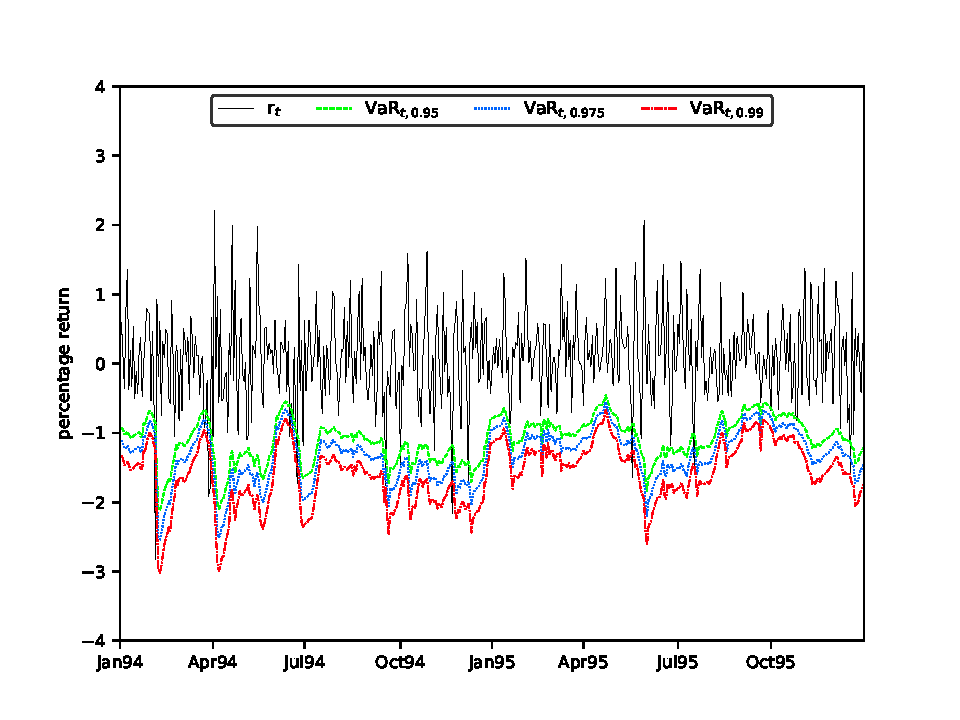
\includegraphics[width=1.2\textwidth, height=0.6\textwidth]{multivar_analysis/tranquil/KNN5_pearson_garch_1994_1995.pdf} 
		\caption{KNN(5)-Pearson-Garch} 	
		\label{fig:KNN(5)-Pearson-Garch}
	\end{subfigure} 
	\hfill	
	\begin{subfigure}[b]{0.33 \textwidth} %3
		\centering 		
		\includegraphics[width=1.2\textwidth, height=0.6\textwidth]{multivar_analysis/tranquil/KNN100_kendall_garch_1994_1995.pdf} 
		\caption{KNN(100)-Kendall-Garch} 
		\label{fig:KNN(100)-Kendall-Garch}
	\end{subfigure}
	\hfill 
	\begin{subfigure}[b]{0.33 \textwidth} %5
		\centering 		
		\includegraphics[width=1.2\textwidth, height=0.6\textwidth]{multivar_analysis/tranquil/KNN_idw_pearson_garch_1994_1995.pdf} 
		\caption{KNN(idw)-Pearson-Garch} 
		\label{fig:KNN(idw)-Pearson-Garch}
	\end{subfigure}
	\hfill   
	\begin{subfigure}[b]{0.33 \textwidth}  %2
		\centering 
		\includegraphics[width=1.2\textwidth, height=0.6\textwidth]{multivar_analysis/tranquil/KNN5_kendall_garch_1994_1995.pdf} 
		\caption{KNN(5)-Kendall-Garch} 
		\label{fig:KNN(5)-Kendall-Garch}
	\end{subfigure} 
	\hfill
	\begin{subfigure}[b]{0.33 \textwidth} %4
		\centering 
		\includegraphics[width=1.2\textwidth, height=0.6\textwidth]{multivar_analysis/tranquil/KNN100_kendall_gjr_1994_1995.pdf} 
		\caption{KNN(100)-Kendall-GJR} 
		\label{fig:KNN(100)-Kendall-GJR}
	\end{subfigure}
	\hfill
	\begin{subfigure}[b]{0.33 \textwidth} %6
		\centering 
		\includegraphics[width=1.2\textwidth, height=0.6\textwidth]{multivar_analysis/tranquil/KNN_idw_kendall_garch_1994_1995.pdf} 
		\caption{KNN(idw)-Kendall-Garch} 
		\label{fig:KNN(idw)-Kendall-Garch}
	\end{subfigure}
	\hfill
	\begin{subfigure}[b]{0.33 \textwidth} %7
		\centering 
		\includegraphics[width=1.2\textwidth, height=0.6\textwidth]{multivar_analysis/tranquil/RF10_pearson_garch_1994_1995.pdf} 
		\caption{RF(10)-Pearson-Garch} 	
		\label{fig:RF(10)-Pearson-Garch}
	\end{subfigure} 
	\hfill
	\begin{subfigure}[b]{0.33 \textwidth}  %8
		\centering 
		\includegraphics[width=1.2\textwidth, height=0.6\textwidth]{multivar_analysis/tranquil/RF10_kendall_garch_1994_1995.pdf} 
		\caption{RF(10)-Kendall-Garch} 
		\label{fig:RF(10)-Kendall-Garch}
	\end{subfigure} 
	\hfill
	\begin{subfigure}[b]{0.33 \textwidth} %11
		\centering 		
		\includegraphics[width=1.2\textwidth, height=0.6\textwidth]{multivar_analysis/tranquil/DCC_garch_mvnorm_1994_1995.pdf} 
		\caption{DCC-Garch} 
		\label{fig:DCC-Garch}
	\end{subfigure}	
	\begin{subfigure}[b]{0.33 \textwidth} %9
		\centering 		
		\includegraphics[width=1.2\textwidth, height=0.6\textwidth]{multivar_analysis/tranquil/RF100_pearson_garch_1994_1995.pdf} 
		\caption{RF(100)-Pearson-Garch} 
		\label{fig:RF(100)-Pearson-Garch}
	\end{subfigure}
	\hfill  
	\begin{subfigure}[b]{0.33 \textwidth} %10
		\centering 
		\includegraphics[width=1.2\textwidth, height=0.6\textwidth]{multivar_analysis/tranquil/RF100_kendall_garch_1994_1995.pdf} 
		\caption{RF(100)-Kendall-Garch} 
		\label{fig:RF(100)-Kendall-Garch}
	\end{subfigure}
	\hfill
	\begin{subfigure}[b]{0.33 \textwidth} %11
		\centering 		
		\includegraphics[width=1.2\textwidth, height=0.6\textwidth]{multivar_analysis/tranquil/DCC_gjr_mvnorm_1994_1995.pdf} 
		\caption{DCC-GJR} 
		\label{fig:DCC-GJR}
	\end{subfigure}	
	\caption[Out-of-sample returns and Value-at-Risk estimates in tranquil market conditions.]{Out-of-sample returns r$_t$ and Value-at-Risk estimates VaR$_{t,\alpha}$ for $\alpha \in \{0.95, 0.975, 0.99\}$ in tranquil market conditions.}
	\label{fig:var_forecasts_tranquil}
\end{figure}
\end{landscape}
\pagestyle{fancy}
\clearpage





\subsection{Volatile Market Conditions: 2000-2001 Dot-com Bubble} \label{sec:volatile}
Table \ref{tab:var_backtest_vol_table} presents an overview of the VaR and CVaR backtest results in volatile market conditions for a long position in an equally weighted portfolio comprising the 30 constituents of the DJIA. The assumption of normality in a volatile market period such as the collapse and aftermath of the Dot-com bubble is unrealistic and results in severe underestimation of true risk, that is, severe underestimation of VaR and CVaR (see tabel \ref{tab:var_backtest_vol_table_dn}). VaR and CVaR are therefore calculated under the assumption that portfolio returns follow a multivariate Student-t distribution, which is better able to capture the fat-tails often exhibited by return distributions in periods of market turmoil. For simplicity, the degrees of freedom of the shape parameter is fixed at the average estimated degrees of freedom of the shape parameter for the initial in-sample period as depicted in tabel \ref{tab:stat_dist_gjr_sstd_table}, that is, 6.9. Similar to the previous section, the backtest results exhibit some general patterns for all three VaR confidence levels considered; (1) semiparametric multivariate volatility models show less conservative behavior compared with the DCC model; (2) semiparametric multivariate volatility models with Kendall approximations of true correlation severely underestimate true risk; (3) the likelihood of a VaR exceedance does not depend greatly on whether a VaR exceedance occurred on the previous day. \\

\noindent
The backtest results indicate that the DCC, KNN(5)-Pearson-GJR, KNN(100)-Pearson, KNN(idw)-Pearson, RF(10)-Pearson and RF(100)-Pearson models are adequate at estimating the 99\% VaR during the (collapse and aftermath of the) Dot-com bubble; the null hypothesis of the unconditional coverage and independence test is not rejected at the 5\% significance level. The  most adequate risk models for the 99\% VaR appear to be the DCC and KNN(100)-Pearson-GJR risk models, which exhibit 5 exceedances against 5 expected exceedances for the 99\% VaR confidence level. The other adequate risk models are slightly less conservative in their estimation of true risk and exhibit 6 exceedances for KNN(100)-Pearson-Garch, KNN(idw)-Pearson-GJR and RF(100)-Pearson to 9 exceedances for RF(10)-Pearson-Garch and KNN(idw)-Kendall-GJR. \\

\noindent
For estimation of the 97.5\% VaR, the backtest results indicate that the DCC, KNN(100)-Pearson, KNN(idw)-Pearson and RF(10)-Pearson are adequate models; the null hypothesis of the unconditional coverage and independence test is not rejected at the 5\% significance level. The remaining models severely underestimate true risk in times of market turmoil, particularly the semiparametric multivariate volatility models with Kendall approximations of true correlation. The  most adequate risk model for the 97.5\% VaR is the DCC-GJR with 14 exceedances while 12.5 exceedances are expected for the 97.5\% VaR confidence level. The KNN(idw)-Pearson is slightly less conservative with an estimated 15 exceedances followed by DCC-Garch, KNN(100)-Pearson and RF(10)-Pearson exhibiting a number of VaR exceedances in the range 16 to 18. Of note is that only the KNN(5)-Kendall risk models reject the null hypothesis of the independence test at the 5\% significance level implying VaR exceedances are not independently distributed in these risk models for the 97\% VaR confidence level. \\

\noindent
The final VaR considered is the 95\% VaR with 25 expected exceedances. We observe similar results compared with the 97.5\% VaR except that the null hypothesis of the unconditional coverage test is rejected for the RF(10)-Pearson risk model this time. This means that DCC, KNN(100) and KNN(idw)-Pearson are adequate risk models for the 95\% VaR. Again, the remaining models severely underestimate true risk in times of market turmoil, particularly the semiparametric multivariate volatility models with Kendall approximations of true correlation. Tabel \ref{tab:var_backtest_volatile_table_lower} indicates that the DCC-Garch, KNN(100)-Pearson and KNN(idw)-Pearson-Garch perform adequate across the entire loss distribution in terms of estimating VaR; the DCC-Garch and KNN(idw)-Pearson-Garch risk models only reject the null hypothesis of the unconditional coverage test at the 5\% significance level for the 0.10 quantile and reject the null hypothesis of the independence test at the 5\% significance level for the 0.01 and 0.90 quantiles of the loss distribution. The KNN(100)-Pearson-Garch risk model only rejects the null hypothesis of the unconditional coverage test at the 5\% significance level for the 0.9 quantile whereas the KNN(100)-Pearson-GJR risk model only rejects the independence test at the 5\% significance level for the 0.01 quantile of the loss distribution. In other words, we have an indication that KNN(100)-Pearson is an adequate risk model specification across more than only the higher quantiles of the loss distribution in terms of estimating VaR in volatile market conditions. The  most adequate risk model for the 97.5\% VaR is the KNN(idw)-Pearson-GJR with 28 exceedances followed by KNN(100)-Pearson with 29 exceedances. The KNN(idw)-Pearson-Garch, DCC-GJR and DCC-Garch have 29, 31 and 33 exceedances, respectively, against an expected 25 exceedances for the 95\% VaR confidence level.  \\

\noindent
The minimum exceedance residual, min($er_t$), for the 99\% VaR is negative for all risk models and corresponds to the suffered losses as a consequence of the September 11 attacks in 2001. This implies that no risk model under consideration ensures that CVaR is never exceeded in the backtest period. Similarly, the mean exceedance residual, mean($er_t$), is also negative for all risk models. This implies that, on average, all risk models under consideration tend to underestimate true CVaR, that is, they tend to underestimate, on average, the actual portfolio loss $L_t$ given that the loss $L_t$ exceeds VaR$_t$. In terms of min($er_t$) and mean($er_t$), the KNN(100)-Pearson-Garch model and KNN(idw)-Pearson-Garch model, respectively, deem the most adequate risk models for the 99\% CVaR.   


\begin{landscape}
\pagestyle{empty}
\begin{table}[h]
\centering
\captionsetup[subtable]{position=below}
\begin{tabular}{l c c c l l l l l l c c}
\toprule
\multicolumn{1}{c}{{\underline{Model}}} & \multicolumn{3}{c}{{\underline{VaR Exceedances}}} & \multicolumn{6}{c}{{\underline{Transition Probabilities}}}  &  \multicolumn{2}{c}{{\underline{CVaR Exceedance Residuals}}}                                                                                   \\
                                & I(0.95)  & I(0.975)  & I(0.99) & \multicolumn{2}{c}{I(0.95)} & \multicolumn{2}{c}{I(0.975)} & \multicolumn{2}{c}{I(0.99)} \\ \cmidrule{2-12} 
                                &             &           &                 & \multicolumn{1}{c}{{$\pi_{01}$}}       & \multicolumn{1}{c}{{$\pi_{11}$}}       & \multicolumn{1}{c}{{$\pi_{01}$}}        & \multicolumn{1}{c}{{$\pi_{11}$}}       & \multicolumn{1}{c}{{$\pi_{01}$}}       & \multicolumn{1}{c}{{$\pi_{11}$}}  & \multicolumn{1}{r}{min($er_t$)}  & \multicolumn{1}{c}{{mean($er_t$)}}       \\  \midrule  
DCC-GARCH				&33		&16		&5        	&0.0601              &0.1212              &0.0311               &0.0625              &0.0101              &0   &-3.922	&-0.7447           \\
DCC-GJR					&31		&14		&5         &0.0577                   &0.0968              &0.0289               &0              &0.0101              &0    &-3.660	&-0.6840          \\ \midrule
KNN(5)-Pearson-Garch            	&\textbf{39}	&\textbf{22}	&\textbf{12}           &0.0696        &0.1538           &0.0398           &0.0909          &0.0205          &0.0833      &-3.672	&-0.3249        \\
KNN(5)-Pearson-GJR              	&\textbf{38}	&\textbf{21}	&9      &0.0672		&0.1579     &0.0397        &0.0476              &0.0184              &0      &-3.807		&-0.6210        \\
KNN(5)-Kendall-Garch           	&\textbf{58}	&\textbf{32}    &\textbf{17}	      &0.1063     &0.1754     &\textbf{0.0535}    &\textbf{0.1875}  	&0.0311      &0.0588   &-4.005	&-0.3459           \\
KNN(5)-Kendall-GJR              	&\textbf{55}	&\textbf{32}	&\textbf{17}          &0.1011      &0.1667    &\textbf{0.0535}	&\textbf{0.1875}         &0.0311              &0.0588      &-4.132	&-0.2994        \\
KNN(100)-Pearson-Garch         &29			&18			&6          &0.0511      &0.1379    &0.0312	&0.1111         &0.0122              &0     &-3.604$^{*}$		&-0.6407         \\
KNN(100)-Pearson-GJR            &29			&17			&5          &0.0511      &0.1379    &0.0311	&0.0588         &0.0101              &0       &-3.732	&-0.9253       \\
KNN(idw)-Pearson-Garch        	&30		&15		&7           &0.0507     &0.0769           &0.0289              &0.0667              &0.0142              &0     &-3.933	&-0.1913$^{*}$         \\
KNN(idw)-Pearson-GJR          	&28		&15		&6                 &0.0552              &0.0714              &0.0289               &0.0667              &0.0122              &0    &-4.044	&-0.4769          \\
KNN(idw)-Kendall-Garch          	&\textbf{43}	&\textbf{21}	&\textbf{10}           &0.0811              &0.1163              &0.0397               &0.0952          &0.0204           &0      &-4.418	 &-0.3828       \\
KNN(idw)-Kendall-GJR            	&\textbf{42}	&\textbf{21}	&9              &0.0788              &0.1190              &0.0397               &0.0952              &0.0184              &0       &-4.515	&-0.5454       \\ \midrule
RF(10)-Pearson-Garch              &\textbf{39}	&18	&9                      &0.0739              &0.1026               &0.0312              &0.1111              &0.0184		&0      &-3.690 	&-0.4632        \\
RF(10)-Pearson-GJR              	&\textbf{38}	&18	&8                &0.0716              &0.1053          &0.0312               &0.1111      &0.0163           &0     &-3.822	   &-0.5804         \\
RF(10)-Kendall-Garch            	&\textbf{54}	&\textbf{28}	&\textbf{15}                &0.1031              &0.1031              &0.0510               &0.1071              &0.031              &0      &-4.395	&-0.3377        \\
RF(10)-Kendall-GJR              	&\textbf{53}	&\textbf{29}	&\textbf{16}            &0.1007              &0.1346              &0.0532               &0.0532         &0.0331              &0     &-4.501	&-0.2881         \\
RF(100)-Pearson-Garch            &\textbf{37}	&\textbf{20}	&6         &0.0671         &0.1351              &\textbf{0.0334}       &\textbf{0.15}       &0.0122              &0   &-3.880	&-0.9040           \\
RF(100)-Pearson-GJR          	&\textbf{36}	&\textbf{20}	&6           &0.0648              &0.1389          &\textbf{0.0334}   	&\textbf{0.15}              &0.0334           &0   &-4.001	&-0.8901           \\
RF(100)-Kendall-Garch           	&\textbf{55}	&\textbf{30}	&\textbf{15}    	&0.1034	&0.1481	&0.0554	&0.1	&0.031	&0      &-4.230		&-0.3161        \\   
RF(100)-Kendall-GJR             	&\textbf{55}	&\textbf{29}	&\textbf{15}         &0.1034        &0.1481              &0.0532               &0.1034             &0.1034          &0    &-4.339		&-0.3463            \\     [1ex]       
\bottomrule  
\end{tabular}
\caption[Backtesting results in volatile market conditions.]{This table presents test results of unconditional coverage (VaR Exceedances), independence (Transition Probabilities) and backtest results of the exceedance residual series (CVaR Exceedance Residuals) at higher quantiles of the loss distribution in volatile market conditions. Bold face indicates rejection. Non-rejection regions for the unconditional coverage test: 15$<$I(0.95)$<$36, 6$<$I(0.975)$<$20 and 0$<$I(0.99)$<$10. Starred entries denote best result on exceedance residual series backtest.} 
\label{tab:var_backtest_vol_table}
\end{table}
\end{landscape}
\pagestyle{fancy}


\noindent
Figure \ref{fig:var_forecasts_volatile} depicts the 95\%, 97.5\% and 99\% VaR estimates of a long position in an equally weighted portfolio in volatile market conditions; in particular, the differences between VaR estimates obtained from the fully parametric DCC model and our semiparametric multivariate volatility model using NN and RF estimators are presented. Figure \ref{fig:var_forecasts_volatile} corroborates our statement that semiparametric multivariate volatility models with Kendall approximations of true correlation exhibit a higher number of VaR exceedances than their Pearson counterpart; estimated VaR levels under Kendall exhibit slightly less volatile behavior and a positive vertical shift compared with their Pearson counterparts. Furthermore, as in the tranquil market period, figure \ref{fig:var_forecasts_volatile} corroborates our discussion from section \ref{sec:mse_decompose} and findings from the simulation study in chapter \ref{ch:simulation_study}; an increase in the number of decision trees in the random forest or an increase in the number of neighbors yields a decrease in the variance of correlation estimates, which results in smoother estimated VaR levels.   \\

\noindent
DCC and KNN(idw)-Pearson model properties result into prudent estimated measures of risk, which is shown by the smooth VaR levels in figures \ref{fig:DCC-Garch}-\ref{fig:DCC-GJR} and figures \ref{fig:KNN(idw)-Pearson-Garch}-\ref{fig:KNN(idw)-Kendall-Garch}, respectively. In times of volatile market conditions such as the 2000-2001 Dot-com bubble, these model properties would be preferred over the properties of semiparametric risk models that more actively, but slow, capture sudden changes in volatility such as KNN(5). In a volatile market conditions, which is characterized by more frequent large losses compared with tranquil market conditions, the delay in capturing volatility changes by the KNN(5) risk model results in overestimation of VaR levels subsequent to isolated large portfolio losses. For example, see the estimated VaR level subsequent to the September 11 attacks in figures \ref{fig:KNN(5)-Pearson-Garch_vol}-\ref{fig:KNN(5)-Kendall-Garch_vol}. An increase in the number of neighbors, such as KNN(100), smooths VaR level estimates because more neighbors are used in the estimation of conditional correlations and captures, although still a bit slow, changing levels of volatility. The random forest estimator with a small number of decision trees such as RF(10) does not suffer from the same undesirable model property as the KNN algorithm with a low number of neighbors because the random forest algorithm uses more sample information for construction of the decision trees. Moreover, conditional correlation estimates are an average of the decision trees' output, which imposes a degree of smoothing on the conditional correlation estimates and, consequently, on the estimated VaR levels.  \\

\noindent
In summary, the most adequate risk models for the 99\% VaR are the DCC and KNN(100)-Pearson-GJR risk models with 5 VaR exceedances against 5 expected. The most adequate risk model for the 97.5\% VaR is the DCC-GJR with 14 exceedances while 12.5 exceedances are expected. The most adequate risk model for the 95\% VaR is the KNN(idw)-Pearson-GJR with 28 exceedances against 25 expected. Of note is that we have an indication that KNN(100)-Pearson, and in particular, KNN(100)-Pearson-GJR, are adequate risk model across more than only the higher quantiles of the loss distribution in terms of estimating VaR in volatile market conditions; the KNN(100)-Pearson-GJR risk model only rejects the independence test at the 5\% significance level for the 0.01 quantile of the loss distribution. In terms of min($er_t$) and mean($er_t$), the KNN(100)-Pearson-Garch model and KNN(idw)-Pearson-Garch model, respectively, deem the most adequate risk models for the 99\% CVaR. 


%%%% VaR figures Volatile Market Conditions  %%%%%
\begin{landscape}
\pagestyle{empty}
\begin{figure}[h] % [h] parameter makes sure figures are located at 'this' location.
	\centering
	\begin{subfigure}[b]{0.33 \textwidth} %1
		\centering 
		\includegraphics[width=1.2\textwidth, height=0.6\textwidth]{multivar_analysis/volatile/KNN5_pearson_garch_2000_2001.pdf} 
		\caption{KNN(5)-Pearson-Garch} 	
		\label{fig:KNN(5)-Pearson-Garch_vol}
	\end{subfigure} 
	\hfill	
	\begin{subfigure}[b]{0.33 \textwidth} %3
		\centering 		
		\includegraphics[width=1.2\textwidth, height=0.6\textwidth]{multivar_analysis/volatile/KNN100_pearson_garch_2000_2001.pdf} 
		\caption{KNN(100)-Pearson-Garch} 
		\label{fig:KNN(100)-Pearson-Garch_vol}
	\end{subfigure}
	\hfill 
	\begin{subfigure}[b]{0.33 \textwidth} %5
		\centering 		
		\includegraphics[width=1.2\textwidth, height=0.6\textwidth]{multivar_analysis/volatile/KNN_idw_pearson_garch_2000_2001.pdf} 
		\caption{KNN(idw)-Pearson-Garch} 
		\label{fig:KNN(idw)-Pearson-Garch_vol}
	\end{subfigure}
	\hfill   
	\begin{subfigure}[b]{0.33 \textwidth}  %2
		\centering 
		\includegraphics[width=1.2\textwidth, height=0.6\textwidth]{multivar_analysis/volatile/KNN5_kendall_garch_2000_2001.pdf} 
		\caption{KNN(5)-Kendall-Garch} 
		\label{fig:KNN(5)-Kendall-Garch_vol}
	\end{subfigure} 
	\hfill	
	\begin{subfigure}[b]{0.33 \textwidth} %4
		\centering 
		\includegraphics[width=1.2\textwidth, height=0.6\textwidth]{multivar_analysis/volatile/KNN100_pearson_gjr_2000_2001.pdf} 
		\caption{KNN(100)-Pearson-GJR} 
		\label{fig:KNN(100)-Pearson-GJR_vol}
	\end{subfigure}
	\hfill
	\begin{subfigure}[b]{0.33 \textwidth} %6
		\centering 
		\includegraphics[width=1.2\textwidth, height=0.6\textwidth]{multivar_analysis/volatile/KNN_idw_kendall_garch_2000_2001.pdf} 
		\caption{KNN(idw)-Kendall-Garch} 
		\label{fig:KNN(idw)-Kendall-Garch_vol}
	\end{subfigure}
	\hfill
	\begin{subfigure}[b]{0.33 \textwidth} %7
		\centering 
		\includegraphics[width=1.2\textwidth, height=0.6\textwidth]{multivar_analysis/volatile/RF10_pearson_garch_2000_2001.pdf} 
		\caption{RF(10)-Pearson-Garch} 	
		\label{fig:RF(10)-Pearson-Garch_vol}
	\end{subfigure} 
	\hfill
	\begin{subfigure}[b]{0.33 \textwidth}  %8
		\centering 
		\includegraphics[width=1.2\textwidth, height=0.6\textwidth]{multivar_analysis/volatile/RF10_kendall_garch_2000_2001.pdf} 
		\caption{RF(10)-Kendall-Garch} 
		\label{RF(10)-Kendall-Garch_vol}
	\end{subfigure} 
	\hfill
	\begin{subfigure}[b]{0.33 \textwidth} %11
		\centering 		
		\includegraphics[width=1.2\textwidth, height=0.6\textwidth]{multivar_analysis/volatile/DCC_garch_mvnorm_2000_2001.pdf} 
		\caption{DCC-Garch} 
		\label{fig:DCC-Garch_vol}
	\end{subfigure}	
	\hfill
	\begin{subfigure}[b]{0.33 \textwidth} %9
		\centering 		
		\includegraphics[width=1.2\textwidth, height=0.6\textwidth]{multivar_analysis/volatile/RF100_pearson_garch_2000_2001.pdf} 
		\caption{RF(100)-Pearson-Garch} 
		\label{fig:RF(100)-Pearson-Garch_vol}
	\end{subfigure}
	\hfill  
	\begin{subfigure}[b]{0.33 \textwidth} %10
		\centering 
		\includegraphics[width=1.2\textwidth, height=0.6\textwidth]{multivar_analysis/volatile/RF100_kendall_garch_2000_2001.pdf} 
		\caption{RF(100)-Kendall-Garch} 
		\label{fig:RF(100)-Kendall-Garch_vol}
	\end{subfigure}
	\hfill
	\begin{subfigure}[b]{0.33 \textwidth} %11
		\centering 		
		\includegraphics[width=1.2\textwidth, height=0.6\textwidth]{multivar_analysis/volatile/DCC_gjr_mvnorm_2000_2001.pdf} 
		\caption{DCC-GJR} 
		\label{fig:DCC-GJR_vol}
	\end{subfigure}	
	\caption[Out-of-sample returns and Value-at-Risk estimates in volatile market conditions.]{Out-of-sample returns r$_t$ and Value-at-Risk estimates VaR$_{t,\alpha}$ for $\alpha \in \{0.95, 0.975, 0.99\}$ in volatile market conditions.}
	\label{fig:var_forecasts_volatile}
\end{figure}
\end{landscape}
\pagestyle{fancy}
\clearpage









\section{Conclusions Empirical Results} \label{sec:conclusions_emp}
In this chapter, we have illustrated the adequacy of our semiparametric multivariate volatility model, using nonparametric k-nearest neighbor and random forest learning estimators for conditional correlation, in terms of estimating downside risk measures Value-at-Risk (VaR) and Conditional Value-at-Risk (CVaR). An empirical application to the 30 constituents included in the Dow Jones Industrial Average index shows competitive performance of the semiparametric multivariate volatility model 
compared with a standard parametric multivariate volatility model, the dynamic conditional correlation (DCC) model of \cite{ref:Engle2002}, both in tranquil market conditions (1994-1995) and volatile market conditions (2000-2001 Dot-com bubble). \\

\noindent
The backtest results exhibit general patterns for the 95\%, 97.5\%, and 99\% VaR confidence levels in both tranquil and volatile market periods; (1) semiparametric risk model specifications show less conservative behavior compared with the DCC risk model; (2) semiparametric risk model specifications with Kendall approximations of true correlation exhibit a higher number of VaR exceedances than their Pearson counterpart; (3) an increase in the number of neighbors in the k-nearest neighbor estimator and an increase in the number of decision trees in the random forest estimator result in increased smoothness of estimated VaR levels; (4) the likelihood of a VaR exceedance does not depend greatly on whether a VaR exceedance occurred on the previous day. \\

\noindent
Defining a single risk model specification that is most adequate for all market conditions and VaR/CVaR confidence levels is a challenging task. Rather, a set of adequate risk models is retrieved from the backtesting process and this set may very well vary with type of backtests, market conditions and VaR/CVaR confidence levels. In practice, the choice for a single risk model from a set of adequate risk models will then largely depend on the decision maker's preference for risk and smoothness of the estimated VaR levels; substantial variation in estimated daily VaR levels changes the risk profile of the held portfolio and it may become infeasible to consistently ensure changing capital requirements are satisfied.  \\

\noindent
For the 95\%, 97.5\%, and 99\% VaR confidence levels in the tranquil market period, the set of risk models deemed adequate comprise KNN(5)-Pearson, KNN(5)-Kendall-Garch, KNN(100)-Kendall, RF(10)-Pearson, RF(10)-Kendall, and RF(100)-Kendall; the null hypothesis of the unconditional coverage and independence test is not rejected at the 5\% significance level for any of these models. On the contrary, for the 95\% VaR, the DCC model rejects the unconditional coverage test at the 5\% significance level for overestimation of true risk. Interestingly, for the 99\% VaR the GJR-GARCH(1,1) model with standard skewed Student t distribution specification for the marginal errors does not improve VaR. The GARCH(1,1) model with standard Gaussian distributional assumption seems sufficiently able to capture the excess kurtosis exhibited by the daily log returns of the 30 DJIA constituents in tranquil market conditions. \\ 
  
\noindent  
A risk averse decision maker who is able to consistently meet capital requirements with variations in estimated VaR levels might prefer RF(10)-Pearson risk model. A slightly less risk averse decision maker interested in smaller variations of estimated VaR levels and adequacy in estimating losses exceeding VaR, that is CVaR, would prefer KNN(100)-Kendall specifications, and in particular the KNN(100)-Kendall-Garch risk model as this model underestimates true portfolio loss the least of all risk models considered in the tranquil market period. Moreover, the KNN(100)-Kendall is an adequate risk model across the entire loss distribution (might the decision maker be interested in the entire distribution of results). Then, decision makers slightly less risk averse might prefer RF(10)-Kendall or RF(100)-Kendall risk models for the 99\% VaR. Lastly, risk loving decision makers might prefer one of the least conservative risk models with a small number of neighbors such as KNN(5)-Pearson or even KNN(5)-Kendall-Garch; these risk models exhibit the lowest capital reserve requirements. However, the substantial variation in estimated VaR levels requires great flexibility from the decision maker to consistently meet capital reserve requirements.   \\

\noindent
For the volatile market period, semiparametric risk models with Kendall approximations of true correlation severely underestimate true risk. Additionally, nearest neighbor estimators with a small number of neighbors such as KNN(5) have been shown slow to timely capture sudden changes in volatility. As such, for the 95\%, 97.5\%, and 99\% VaR confidence levels in the volatile market period, the set of adequate risk models comprises more conservative risk models with Pearson approximations of true correlation: DCC, KNN(100)-Pearson and KNN(idw)-Pearson. The RF(10)-Pearson is a risk model to consider for the 97.5\%, and 99\% VaR but underestimates true risk for 95\% VaR. Of note, the GJR-GARCH(1,1) model with standard skewed Student t distribution specification for the marginal errors proves a more adequate choice for the conditional volatility model than the GARCH(1,1) model with standard Gaussian distribution specification for the marginal errors; as expected, DCC-GJR, KNN(100)-Pearson-GJR and KNN(idw)-Pearson-GJR better capture the excess kurtosis and skewness exhibited by the daily log returns of the 30 DJIA constituents in market turmoil than their GARCH counterparts. Although both conditional variance specifications tend to slightly underestimate true risk in the volatile market period, the adequate risk models with GJR specifications produces a number of VaR exceedances closer to the expected number of VaR exceedances for the 95\%, 97.5\%, and 99\% VaR confidence levels. \\

\noindent
The differences between the adequate risk models for the volatile market period are very subtle. The DCC and KNN(idw)-Pearson risk models exhibit a very similar (high) degree of smoothness in their estimated VaR levels compared with the slightly more volatile estimated VaR levels of the KNN(100)-Pearson risk model. For the 99\% VaR, a conservative decision maker might prefer the DCC-Garch, DCC-GJR or KNN(100)-Pearson-GJR risk model, which all exhibit 5 VaR exceedances where 5 are expected. A slightly less conservative decision maker might prefer the KNN(idw)-Pearson-Garch or KNN(idw)-Pearson-GJR risk model, which exhibit 7 and 6 exceedances, respectively. Similar subtle differences hold for the 95\% and 97.5\% VaR confidence levels. A decision maker interested in adequacy of the risk model across the entire loss distribution would certainly prefer KNN(100)-Pearson-GJR; this model only rejects the null hypothesis of the independence test at the 5\% significance level for the 0.01 quantile. In contrast, the other risk models that are deemed adequate at higher quantiles of the loss distribution show several rejections of the null hypothesis of the unconditional coverage or independence test or a mixture of both for the lower quantiles of the loss distribution. Lastly, a decision maker interested in the risk model's adequacy in terms of estimating losses exceeding VaR, that is CVaR, would prefer KNN(idw)-Pearson-Garch as this risk model underestimates, on average, true portfolio loss the least of all risk models considered in the volatile market period.



\chapter{Conclusions and Future Research} \label{ch:conclusion}
The aim of this paper was to develop a new semiparametric model for the conditional covariance matrix that is flexible and remains easy to estimate in high dimensional systems. We have shown that the integration of statistical models for capturing conditional volatility, such as univariate GARCH-type models, with nonparametric machine learning estimators k-nearest neighbor and random forest for the conditional correlations provides a flexible, semiparametric way of formulating multivariate volatility models that avoid the imposition of (potentially misspecified) assumptions on the distribution and functional form of the conditional correlation matrix. Conditional correlations are only assumed to depend on lagged minimum and maximum log return and Pearson and Kendall sample correlations obtained using moving window estimation. \\

\noindent
The proposed semiparametric multivariate volatility model was applied to the 30 constituents included in the Dow Jones Industrial Average index and performance was verified in terms of  economic loss functions Value-at-Risk and Conditional Value-at-Risk. It has been demonstrated that the model is able to capture interesting conditional properties in correlations and that it is competitive with a fully parametric counterpart, both in tranquil market conditions such as the mid-1990's and volatile market conditions during the 2000-2001 Dot-com bubble. This work has therefore provided initial insights in the successful use of k-nearest neighbor and random forest learning estimators for estimation of conditional correlation between financial returns. Proposed semiparametric multivariate volatility model may hence be considered in the context of downside market risk assesment. \\

\noindent 
The adequate results of proposed semiparametric multivariate volatility model are however not limited to the specific case of downside market risk assessment and may be extended to other topics in the field of financial econometrics. For future research, it may be interesting to apply proposed semiparametric multivariate volatility model for estimation of the conditional variance-covariance matrix in the context of a multi-stage portfolio optimization problem. It would be interesting to examine proposed semiparametric model's ability to capture multi-stage conditional properties in correlations and volatilities.    


\bibliographystyle{plainnat}
\bibliography{refThesis}

%%%%%%%%%%%%%%%%%%%%%%%%%%%%%%%%%%%%%%%%%%%%%%%%%%%%%%%%%%%%%%
%%%%%%%%%%%%%%%%					APPENDIX						    %%%%%%%%%%%
%%%%%%%%%%%%%%%%%%%%%%%%%%%%%%%%%%%%%%%%%%%%%%%%%%%%%%%%%%%%%%
% Activate the appendix
% from now on sections are numerated with capital letters
\appendix

\chapter{Descriptive Statistics DJIA}
\begin{table}[H]
\centering
\captionsetup[subtable]{position=below}
\scalebox{0.85} {
\begin{tabular}{l c c c c c c c}
\toprule
\multicolumn{1}{ c }{\textbf{Asset}} &
\multicolumn{1}{ r }{\textbf{Mean}} &
\multicolumn{1}{ r }{\textbf{St. dev}} &
\multicolumn{1}{ r }{\textbf{Skewness}} &
\multicolumn{1}{ r }{\textbf{Ex. kurtosis}} &
\multicolumn{1}{ r }{\textbf{Minimum}} &
\multicolumn{1}{ r }{\textbf{Maximum}} &
\multicolumn{1}{ c }{\textbf{Jarque-Bera}}  \\
\midrule 
AA    & 0.0601 & 2.071   & -0.4802  & 11.36        & -27.46  & 13.13   & 20172  \\
AXP   & 0.0407 & 2.272   & -0.7064  & 11.99        & -30.34  & 17.12   & 22613  \\
BA    & 0.0402 & 1.964   & -0.5576  & 9.10         & -19.39  & 14.22   & 13054  \\
BAC   & 0.0562 & 2.070   & -0.2483  & 5.21         & -20.76  & 10.88   & 4253   \\
C     & 0.0747 & 2.328   & -0.6653  & 10.27        & -26.43  & 16.85   & 16638  \\
CAT   & 0.0481 & 2.054   & -0.5227  & 9.08         & -24.42  & 13.59   & 12963  \\
CVX   & 0.0478 & 1.549   & -0.4946  & 8.06         & -18.13  & 9.04    & 10232  \\
DD    & 0.0359 & 1.812   & -0.3979  & 6.45         & -20.19  & 8.37    & 6551   \\
DIS   & 0.0413 & 2.074   & -1.3173  & 27.44        & -34.26  & 17.56   & 117944 \\
GE    & 0.0689 & 1.713   & -0.4117  & 8.00         & -19.47  & 11.75   & 10041  \\
GM    & 0.0282 & 1.984   & -0.4274  & 7.61         & -23.63  & 13.71   & 9091   \\
HD    & 0.1224 & 2.334   & -1.2136  & 18.04        & -33.86  & 12.14   & 51412  \\
HPQ   & 0.0389 & 2.638   & -0.2964  & 6.21         & -22.64  & 15.91   & 6031   \\
IBM   & 0.0417 & 2.009   & -0.6378  & 14.46        & -26.82  & 12.36   & 32714  \\
INTC  & 0.1009 & 2.897   & -0.4263  & 6.08         & -24.89  & 22.65   & 5846   \\
JNJ   & 0.0704 & 1.660   & -0.4638  & 8.20         & -20.44  & 10.57   & 10564  \\
JPM   & 0.0422 & 2.314   & -0.6260  & 13.22        & -32.35  & 14.77   & 27356  \\
AIG   & 0.0694 & 1.701   & -0.2275  & 5.21         & -17.19  & 10.48   & 4247   \\
KO    & 0.0624 & 1.797   & -0.7580  & 21.66        & -28.29  & 17.91   & 73197  \\
MCD   & 0.0417 & 1.745   & -0.3339  & 6.20         & -18.28  & 10.31   & 6039   \\
MMM   & 0.0488 & 1.586   & -0.8289  & 14.45        & -22.58  & 10.50   & 32827  \\
MRK   & 0.0600 & 1.735   & -0.1886  & 3.56         & -13.93  & 9.27    & 1988   \\
MSFT  & 0.1271 & 2.602   & -0.9667  & 16.21        & -37.95  & 17.85   & 41368  \\
PFE   & 0.0772 & 1.942   & -0.3331  & 4.48         & -18.92  & 9.89    & 3182   \\
PG    & 0.0608 & 1.837   & -3.1385  & 68.07        & -35.99  & 19.80   & 725300 \\
T     & 0.0523 & 1.705   & -0.1757  & 3.85         & -13.52  & 10.67   & 2314   \\
UTX   & 0.0530 & 1.827   & -1.5147  & 24.37        & -30.29  & 9.87    & 93592  \\
VZ    & 0.0435 & 1.679   & -0.1381  & 8.58         & -19.31  & 13.18   & 11430  \\
WMT   & 0.0769 & 2.054   & -0.0796  & 2.69         & -12.50  & 11.47   & 1128   \\
XOM   & 0.0511 & 1.528   & -1.0537  & 30.83        & -26.77  & 16.54   & 148221 \\ [1ex]
\bottomrule  
\end{tabular}
}
\caption[Descriptive statistics of Dow Jones Industrial Average daily log returns.]{Descriptive statistics of Dow Jones Industrial Average daily log returns. Tick symbol is used to denote the company and critical value of the Jarque-Bera test statistic is 5.99. Log returns are in percentages and the sample period is from March 1987 to December 2001 for 3735 observations.} 
\label{tab:stats_data}
\end{table}

\chapter{Cross-sectional Distribution Data of Conditional Variance Models}

\begin{table}[H]
\centering
\captionsetup[subtable]{position=below}
\begin{tabular}{l c c c c c c c}
\toprule
\multirow{2}{*}{}      & \multicolumn{7}{c}{Cross-sectional distribution}                                        \\ \cmidrule{3-8} 
                    &   & Mean       & 5\%       & 25\%      & Median    & 75\%               & 95\%              \\ \midrule 
$\omega_i$         &        & 0.1767     & 0.0231    & 0.0696    & 0.1167    & 0.2150             & 0.5559            \\
$\alpha_i$           &       & 0.0853     & 0.0340    & 0.0589    & 0.0806    & 0.1054             & 0.1421            \\
$\beta_i$             &     & 0.8716     & 0.7817    & 0.8434    & 0.8764    & 0.9153             & 0.9565            \\
\multicolumn{6}{l}{}                                                    & \multicolumn{2}{l}{No. of  Rejections} \\
\multicolumn{6}{l}{LB test for standardized residuals}                  & \multicolumn{2}{c}{1}                  \\
\multicolumn{6}{l}{WP test for squared standardized residuals} & \multicolumn{2}{c}{2}                  \\
\multicolumn{6}{l}{KS test for Gaussian dist standardized residuals}      & \multicolumn{2}{c}{30}     \\ [1ex]            
\bottomrule  
\end{tabular}
\caption[Summary statistics of GJR-GARCH Gaussian model specification for the conditional variance in volatile market conditions.]{Summary statistics of the estimated ARMA(3,1)-GARCH(1,1) model with Gaussian marginal distribution on daily log returns of 30 constituents included in the Dow Jones Industrial Average index for the period March 1987 to December 1999 for 3235 observations. The columns present the mean and quantiles from the cross-sectional distribution of the parameters listed in the rows. Results from Goodness-of-fit tests are shown in the bottom of the table. The first and second row present the number of rejections (at the 0.05 level) across 30 assets from Ljung-Box and weighted portmanteau tests for autocorrelation up to the tenth lag for standardized residuals and squared standardized residuals, respectively. The bottom row shows the number of rejections across 30 assets from a Kolmogorov-Smirnov test of the the Gaussian distribution fit to the standardized residuals.} 
\label{tab:stat_dist_garch_norm_table}
\end{table}

\begin{table}[H]
\centering
\captionsetup[subtable]{position=below}
\begin{tabular}{l c c c c c c c}
\toprule
\multirow{2}{*}{}      & \multicolumn{7}{c}{Cross-sectional distribution}                                        \\ \cmidrule{3-8} 
                    &   & Mean       & 5\%       & 25\%      & Median    & 75\%               & 95\%              \\ \midrule 
$\omega_i$         &        & 0.1669	&0.0255	&0.0570	&0.0996	&0.2281	&0.4698            \\
$\alpha_i$           &       &0.0430		 &0.0039	 &0.0289	 &0.0405	 &0.0529	 &0.0883            \\
$\beta_i$             &     & 0.8884		& 0.7721	& 0.8464	& 0.9132	& 0.9299	& 0.9560            \\
$\gamma_i$        &     & 0.0443		&0.0073	&0.0179	&0.0412	&0.0671	&0.1001            \\
$v_i$                  &   & 6.1283	 & 4.8735 		 & 5.2661	 & 5.8752		 & 6.4095		 & 8.4389            \\
$\psi_i$               &     & 1.0288		 &0.9797	 &1.0150	 &1.0314	 &1.0443	 &1.0698            \\
\multicolumn{6}{l}{}                                                    & \multicolumn{2}{l}{No. of  Rejections} \\
\multicolumn{6}{l}{LB test for standardized residuals}                  & \multicolumn{2}{c}{1}                  \\
\multicolumn{6}{l}{WP test for squared standardized residuals} & \multicolumn{2}{c}{1}                  \\
\multicolumn{6}{l}{KS test for skew t dist standardized residuals}      & \multicolumn{2}{c}{3}     \\ [1ex]            
\bottomrule  
\end{tabular}
\caption[Summary statistics of GJR-GARCH skewed Student's t model specification for the conditional variance in tranquil market conditions.]{Summary statistics of the estimated ARMA(3,1)-GARCH(1,1) model with skewed Student's t marginal distribution on daily log returns of 30 constituents included in the Dow Jones Industrial Average index for the period March 1987 to December 1993 for 1720 observations. The columns present the mean and quantiles from the cross-sectional distribution of the parameters listed in the rows. Goodness-of-fit test results are shown in the bottom of the table. The first and second row present the number of rejections (at the 0.05 level) across 30 assets from Ljung-Box and weighted portmanteau tests for autocorrelation up to the tenth lag for standardized residuals and squared standardized residuals. The bottom row shows the number of rejections across 30 assets from a Kolmogorov-Smirnov test of the Gaussian distribution fit to the standardized residuals.} 
\label{tab:stat_dist_gjr_sstd_tranquil_table}
\end{table}

\begin{table}[H]
\centering
\captionsetup[subtable]{position=below}
\begin{tabular}{l c c c c c c c}
\toprule
\multirow{2}{*}{}      & \multicolumn{7}{c}{Cross-sectional distribution}                                        \\ \cmidrule{3-8} 
                    &   & Mean       & 5\%       & 25\%      & Median    & 75\%               & 95\%              \\ \midrule 
$\omega_i$         &        & 0.3199	&0.0453	&0.0938	&0.1875	&0.3947	&1.0375            \\
$\alpha_i$           &       & 0.1263	 & 0.0556	 & 0.0765	 & 0.1083	 & 0.1480	 & 0.2322            \\
$\beta_i$             &     & 0.7906		&0.5927	&0.7519	&0.8132	&0.8853	&0.9262            \\
\multicolumn{6}{l}{}                                                    & \multicolumn{2}{l}{No. of  Rejections} \\
\multicolumn{6}{l}{LB test for standardized residuals}                  & \multicolumn{2}{c}{1}                  \\
\multicolumn{6}{l}{WP test for squared standardized residuals} & \multicolumn{2}{c}{1}                  \\
\multicolumn{6}{l}{KS test for Gaussian dist standardized residuals}      & \multicolumn{2}{c}{26}     \\ [1ex]            
\bottomrule  
\end{tabular}
\caption[Summary statistics of GJR-GARCH Gaussian model specification for the conditional variance in tranquil market conditions.]{Summary statistics of the estimated ARMA(3,1)-GARCH(1,1) model with Gaussian marginal distribution on daily log returns of 30 constituents included in the Dow Jones Industrial Average index for the period March 1987 to December 1993 for 1720 observations. The columns present the mean and quantiles from the cross-sectional distribution of the parameters listed in the rows. Goodness-of-fit test results are shown in the bottom of the table. The first and second row present the number of rejections (at the 0.05 level) across 30 assets from Ljung-Box and weighted portmanteau tests for autocorrelation up to the tenth lag for standardized residuals and squared standardized residuals. The bottom row shows the number of rejections across 30 assets from Kolmogorov-Smirnov test of the Gaussian distribution fit to the standardized residuals.} 
\label{tab:stat_dist_garch_norm_tranquil_table}
\end{table}

\chapter{Value-at-Risk Estimates on Lower Quantiles} \label{ap:var}

\pagestyle{empty}
\begin{landscape}
\begin{table}[h]
\centering
\captionsetup[subtable]{position=below}
%\captionsetup[table]{position=below}
\begin{tabular}{l  l  l  l l l l l l l} 
\toprule
\multicolumn{1}{ c }{\underline{Model}} &
\multicolumn{1}{ c }{{I(0.01)}} &
\multicolumn{1}{ c }{{I(0.025)}} &
\multicolumn{1}{ c }{{I(0.05)}} &
\multicolumn{1}{ c }{{I(0.10)}} &
\multicolumn{1}{ c }{{I(0.20)}} &
\multicolumn{1}{ c }{{I(0.40)}} &
\multicolumn{1}{ c }{{I(0.60)}} &
\multicolumn{1}{ c }{{I(0.80)}} &
\multicolumn{1}{ c }{{I(0.90)}}  \\
\midrule 

DCC-Garch	  &\textbf{504}(0)  	&\textbf{501}(0.04)	&\textbf{495}(0.33)		&\textbf{476}(3.30) 		&\textbf{444}(0.58) 	&320(2.36) 		&\textbf{164}(0.26)		&\textbf{48}(0.72)	&\textbf{14}(1.44) 	\\
DCC-GJR		&\textbf{504}(0)  	&\textbf{501}(0.04)	&\textbf{494}(0.41)		&\textbf{475}(3.55) 		&\textbf{446}(0.31) 	&321(1.95) 		&\textbf{164}(0.26)		&\textbf{48}(0.72)	&\textbf{16}(0.40) 			\\ \midrule 
KNN(5)-Pearson-Garch  	  &498(0.14)	&491	(0.69)	&476	(0.25)	&450	(0.01)	&420	(0.87)	&303(3.43)		&184	(0)	&\textbf{77}(0.56)	   &\textbf{34}(2.86)     \\
KNN(5)-Pearson-GJR      	  &498(0.14)	&491	(0.69)	&473	(0.58)	&449	(0)	&415	(1.61)	&298(2.74)		&186(0)	&\textbf{80}(0.56)	   &39(\textbf{4.75})    \\
KNN(5)-Kendall-Garch   	  &\textbf{491}(0.69)		&\textbf{482}(2.01)		&\textbf{467}(1.62)		&444(1.34)		&408(0.58)		&294	(\textbf{5.09})	&193(0)	&92(0.12)		&48(2.66)  \\
KNN(5)-Kendall-GJR  	  &\textbf{489}(0.92)		&\textbf{480}(2.41)		&\textbf{463}(1.75)		&442(1.75)		&405(0.18)		&289(\textbf{7.00})	&194(0.02)	&94(0.17)	&49(2.32) 	\\
KNN(100)-Kendall-Garch    &502(0.02)	&490(0.80)		&478	(2.84)	&456(2.16)		&413(1.09)		&298(3.39)		&189(0.14)		&84(0.39)		&39(1.31)	\\
KNN(100)-Kendall-GJR       &501(0.04)	&488(1.05)		&475	(3.55)	&452(3.30)		&408(0.58)		&296(\textbf{4.58})		&191(0.08)		&87(0.36)		&40(1.08)  \\
KNN(idw)-Pearson-Garch      &\textbf{504}(0)		&\textbf{501}(0.04)		&\textbf{495}(0.33)		&\textbf{476}(3.30)		&\textbf{444}(0.58)		&320	(2.36)	   &\textbf{164}(0.26)	&\textbf{49}(0.01)	&\textbf{14}(0.72)	\\
KNN(idw)-Pearson-GJR       &\textbf{504}(0)		&\textbf{500}(0.06)		&\textbf{495}(0.33)		&\textbf{475}(3.55)		&\textbf{443}(0.43)		&318	(2.62)	   &\textbf{165}(0.14)	&\textbf{52}(0.57)	&\textbf{16}(0.40) \\
KNN(idw)-Kendall-Garch 	   &501(0.04)		&496	(0.26)	&487	(1.19)	&\textbf{467}(\textbf{5.88})		&\textbf{432}(0.91)		&308(2.26)		&\textbf{175}(0.03)		&\textbf{61}(1.10)		&\textbf{27}(0.17) \\
KNN(idw)-Kendall-GJR 	 &500(0.06)		&496	(0.26)	&483(1.83)	&464(\textbf{6.92})		&\textbf{429}(0.39)		&304(3.58)		&\textbf{179}(0.02)		&\textbf{70}(1.37)  &\textbf{30}(0.03) \\ \midrule
RF(10)-Pearson-Garch  	   &\textbf{503}(0)		&\textbf{499}(0.10)	&482(2.01)		&\textbf{467}(\textbf{5.88})	&\textbf{429}(0.39)	&305	(2.43)	&\textbf{178}(0.15)		&\textbf{72}(2.66)      &\textbf{26}(0.31)                  \\ 
RF(10)-Pearson-GJR     &\textbf{503}(0)		&496(0.26)	&479(2.62)		&465(\textbf{6.56})	&\textbf{423}(0.40)	&303	(1.66)	&182(0.13)		&\textbf{75}(1.68)      &\textbf{29}(0.99)                  \\
RF(10)-Kendall-Garch 	   &498(0.14)		&488(1.05)		&473(\textbf{4.07})		&452	(1.50)	&411(0.28)		&295(\textbf{4.43})		&192(0)		&\textbf{83}(0.17)	&42(0.17)	  \\ 
RF(10)-Kendall-GJR      &497(0.20)		&484(1.66)		&471(\textbf{4.64})		&448	(0.01)	&406(0.29)		&291(\textbf{6.38})		&192(0)		&86(0.01)	&46(0.84)	 \\
RF(100)-Pearson-Garch	&\textbf{504}(0)		&\textbf{499}(0.10)		&483(1.83)		&466	(\textbf{6.22})	&\textbf{427}(0.56)		&308	(1.73)	&\textbf{178}(0.15)		&\textbf{68}(3.03)      &\textbf{25}(0.44)	\\
RF(100)-Pearson-GJR  &\textbf{503}(0)		&497(0.20)		&480(2.41)		&465(\textbf{6.56})	&\textbf{423}(0.91)		&303	(1.66)	&181(0)		&\textbf{71}(1.98)      &\textbf{30}(2.38) \\
RF(100)-Kendall-Garch	&500	(0.06)	&486	(1.34)	&473(\textbf{4.07})		&454(1.09)		&407(0.86)		&296	(\textbf{4.58})	&191(0.01)		&85(0.26)		&42(1.80)		\\ 
RF(100)-Kendall-GJR  &499(0.10)	&485(1.49)	&470(\textbf{4.93})		&452(0.47)		&406(0.66)		&291(\textbf{6.38})	&191(0.01)		&86(0.16)		&47(0.66)	\\  [1ex]
\bottomrule
\end{tabular}
\caption[Backtesting results on lower quantiles in tranquil market conditions.]{This table presents test results of unconditional coverage (VaR Exceedances) and independence (Log-likelihood Ratio between parentheses) at lower quantiles of the loss distribution in tranquil market conditions. Bold face indicates rejection. Non-rejection regions: 494$<$I(0.01)$<$503, 483$<$I(0.025)$<$498, 468$<$I(0.05)$<$489, 439$<$I(0.10)$<$467, 384$<$I(0.20)$<$421, 280$<$I(0.40)$<$325, 180$<$I(0.60)$<$224, 83$<$I(0.80)$<$120 and 37$<$I(0.90)$<$65.}
\label{tab:var_backtest_tranquil_table_lower}
\end{table}
\end{landscape}


%%%   VOLATILE MARKET CONDITIONS 
\pagestyle{empty}
\begin{landscape}
\begin{table}[h]
\centering
\captionsetup[subtable]{position=below}
%\captionsetup[table]{position=below}
\begin{tabular}{l  l  l  l l l l l l l} 
\toprule
\multicolumn{1}{ c }{\underline{Model}} &
\multicolumn{1}{ c }{{I(0.01)}} &
\multicolumn{1}{ c }{{I(0.025)}} &
\multicolumn{1}{ c }{{I(0.05)}} &
\multicolumn{1}{ c }{{I(0.10)}} &
\multicolumn{1}{ c }{{I(0.20)}} &
\multicolumn{1}{ c }{{I(0.40)}} &
\multicolumn{1}{ c }{{I(0.60)}} &
\multicolumn{1}{ c }{{I(0.80)}} &
\multicolumn{1}{ c }{{I(0.90)}}  \\
\midrule 
DCC-Garch	  &495(\textbf{4.48})	&490(1.75)	&482(0.18)	&\textbf{465}(0.10)		&406(0.65)	&311(0.07)	&212(0.48)	&102(0.18)	&60(\textbf{4.04})	\\
DCC-GJR	 &496(0.06)	&491(2.13)	&\textbf{484}(0.39)		&\textbf{466}(1.06)		&406(1.23)	&311(0.07)	&211(0.72)	&104(0.01)	&60(\textbf{4.04}) \\ \midrule 
KNN(5)-Pearson-Garch  	  &495(0.10)	&487(0.91)		&477(0)		&451(0.18)		&396(1.68)		&305(0.28)		&217(1.40)		&\textbf{121}(1.55)	  	&\textbf{72}(\textbf{7.31})   \\
KNN(5)-Pearson-GJR    &494(3.71)	&487(0.91)		&478(0)		&452(0.10)		&397(1.41)		&305(0.28)		&216(1.81)		&\textbf{118}(1.27)	  	&\textbf{72}(\textbf{5.65})    \\
KNN(5)-Kendall-Garch 	  &492(2.57)	&\textbf{480}(0.05)		&\textbf{464}(0.17)		&438(0.09)		&383(0.37)	&300(0.12)	&220(1.57)	&\textbf{135}(0.12)	&\textbf{87}(2.48)  		\\
KNN(5)-Kendall-GJR  	&492(2.57)	&\textbf{480}(0.05)		&\textbf{464}(0.17)		&438(0.09)		&384(0.25)	&302(0.41)	&221(1.19)	&\textbf{133}(0.50)	&\textbf{84}(\textbf{4.93}) \\
KNN(100)-Pearson-Garch  &498(0.02)		&489(1.43)	&483(0.27)	&458(0.10)	&405(0.83)	&309(0.03)	&212(0.77)	&109(0.03)	&\textbf{66}(0.94)	\\
KNN(100)-Pearson-GJR 	&497(\textbf{6.80})		&488(1.15)	&483(0.27)	&459(0.05)	&409(0.63)	&306(0.45)	&211(1.07)	&108(0)	&63(1.68) \\
KNN(idw)-Pearson-Garch      &495(\textbf{4.48})		&492(2.57)	&482(0.18)	&\textbf{466}(1.06)	&405(0.38)	&311(0.07)	&211(0.44)	&101(0.29)	&59(\textbf{4.51})		\\
KNN(idw)-Pearson-GJR    &494(3.71)		&491(2.13)	&\textbf{484}(0.39)		&\textbf{468}(0.74)		&407(0.49)	&311(0.07)	&207(0.53)	&100(0.14)	&59(3.03)	\\
KNN(idw)-Kendall-Garch  	   &493(3.09)	&486(0.71)		&475(0.06)		&449(0.37)		&394(0.02)		&304(0.03)		&215(0.35)		&\textbf{122}(1.26) &\textbf{73}(2.56)		\\
KNN(idw)-Kendall-GJR   &493(3.09)	&486(0.71)	&476(0.02)	&446(0.27)	&393(0.06)	&302(0.07)	&215(0.35)	&\textbf{119}(0.27)		&\textbf{72}(1.89)	 \\ \midrule 
RF(10)-Pearson-Garch     &494(3.71)	 &487(0.91)	 &476(0.02)	&454(0.02)		 &398(1.87)	 &307(0.20)	 &213(0.82)	 &117(0.57)	&\textbf{71}(2.21)              \\ 
RF(10)-Pearson-GJR    &493(3.09)	 &486(0.71)	 &476(0.02)	&453(0.05)		 &399(1.59)	 &306(0.45)	 &213(0.82)	 &117(1.00)	&\textbf{69}(2.93)   \\
RF(10)-Kendall-Garch   	   &491(2.13)		&484(0.39)		&468(0.74)		&\textbf{433}(0.15)		&387(0.17)		&302(0.07)		&220(1.14)	&\textbf{134}(0.34)	&\textbf{82}(2.38)	  \\ 
RF(10)-Kendall-GJR    &\textbf{490}(1.75)		&484(0.39)		&470(0.74)		&\textbf{431}(0.35)		&389(0.19)		&302(0.07)		&220(1.14)	&\textbf{135}(0.47)	&\textbf{80}(2.13)\\
RF(100)-Pearson-Garch 	   &496(\textbf{5.46})	&488(1.15)	&478(0)	&454(0.02)	&396(1.03)	&305(0.28)	&212(0.77)	&117(0.26)  	&\textbf{69}(2.93) \\
RF(100)-Pearson-GJR	 &496(\textbf{5.46})		&488(1.15)	&479(0.02)	&454(0.02)	&399(0.47)	&306(0.45)	&212(0.77)	&116(0.39)  	&\textbf{68}(3.33)   \\
RF(100)-Kendall-Garch   	   &\textbf{490}(1.75)		&484(0.39)	&468(0.45)	&\textbf{435}(0.35)	&387(0.02)	&300(0)	&218(0.71)	&\textbf{136}(0.31)	&\textbf{81}(2.75)		\\			
RF(100)-Kendall-GJR  	&\textbf{490}(1.75)		&484(0.39)	&471(0.06)	&\textbf{434}(0.08)		&387(0.17)	&301(0.01)	&218(0.71)	&\textbf{134}(0.34)		&\textbf{80}(3.14)			\\ [1ex]
\bottomrule
\end{tabular}
\caption[Backtesting results on lower quantiles in volatile market conditions.]{This table presents test results of unconditional coverage (VaR Exceedances) and independence (Log-likelihood Ratio between parentheses) at lower quantiles of the loss distribution in volatile market conditions. Bold face indicates rejection. Non-rejection regions: 490$<$I(0.01)$<$500, 480$<$I(0.025)$<$494, 464$<$I(0.05)$<$484, 435$<$I(0.10)$<$463, 381$<$I(0.20)$<$418, 278$<$I(0.40)$<$322, 178$<$I(0.60)$<$222 and 82$<$I(0.80)$<$118 and and 37$<$I(0.90)$<$65.}
\label{tab:var_backtest_volatile_table_lower}
\end{table}
\end{landscape}


\chapter{Delta-Normal Method in Volatile Market Conditions}
\pagestyle{empty}
\begin{landscape}
\begin{table}[h]
\centering
\captionsetup[subtable]{position=below}
\begin{tabular}{l c c c  l l l l l l l l}
\toprule
\multicolumn{1}{c}{{\underline{Model}}} & \multicolumn{3}{c}{{\underline{VaR Exceedances}}} & \multicolumn{6}{c}{{\underline{Transition Probabilities}}}                                                                     \\
                                & I(0.95)  & I(0.975)  & I(0.99) & \multicolumn{2}{c}{I(0.95)} & \multicolumn{2}{c}{I(0.975)} & \multicolumn{2}{c}{I(0.99)} \\ \cmidrule{2-10} 
                                &             &           &                 & \multicolumn{1}{c}{{$\pi_{01}$}}       & \multicolumn{1}{c}{{$\pi_{11}$}}       & \multicolumn{1}{c}{{$\pi_{01}$}}        & \multicolumn{1}{c}{{$\pi_{11}$}}       & \multicolumn{1}{c}{{$\pi_{01}$}}       & \multicolumn{1}{c}{{$\pi_{11}$}}       \\  \midrule  
DCC-GARCH					&28		&16		&9        	&0.0531              &0.1071              &0.0311               &0.0625              &0.0184              &0              \\
DCC-GJR					        &29		&17		&8         &0.0532                   &0.1034              &0.0311               &0.1176              &0.0163              &0              \\ \midrule
KNN(5)-Pearson-Garch            	&34	&\textbf{23}	&\textbf{16}                &\textbf{0.0581}        &\textbf{0.1765}           &0.0420           &0.0870          &0.0290          &0.0625              \\
KNN(5)-Pearson-GJR              	&34	&\textbf{24}	&\textbf{15}      &\textbf{0.0581}	&\textbf{0.0581}     &0.0442        &0.0833              &0.0269              &0.0667              \\
KNN(5)-Kendall-Garch           	&\textbf{53}	&\textbf{32}    &\textbf{20}	      &0.0984     &0.1538     &\textbf{0.0535}    &\textbf{0.1875}  	&0.0355      &0.1              \\
KNN(5)-Kendall-GJR              	&\textbf{51}	&\textbf{32}	&\textbf{20}          &0.0958      &0.14    &\textbf{0.0535}	&\textbf{0.1875}         &0.0376              &0.05              \\
KNN(idw)-Pearson-Garch        	&26		&15		&9           &0.0507     &0.0769           &0.0289              &0.0667              &0.0184              &0              \\
KNN(idw)-Pearson-GJR          	&27	&15	&9                 &0.053              &0.0741              &0.0289               &0.0667              &0.0184              &0              \\
KNN(idw)-Kendall-Garch          	&\textbf{42}	&\textbf{25}	&\textbf{15}           &0.0788              &0.119              &0.0485               &0.08          &0.0289           &0.0667              \\
KNN(idw)-Kendall-GJR            	&\textbf{41}	&\textbf{23}	&\textbf{15}              &0.0764              &0.122              &0.0441               &0.087              &0.0289              &0.0667              \\ \midrule
RF(10)-Pearson-Garch              &\textbf{37}	&18	&\textbf{10}                      &0.0693              &0.1081               &0.0312              &0.1111              &0.0204	&0              \\
RF(10)-Pearson-GJR              	&\textbf{36}	&18	&\textbf{11}                &0.067              &0.1111          &0.0312               &0.1111      &0.0225           &0              \\
RF(10)-Kendall-Garch            	&\textbf{50}	&\textbf{33}	&\textbf{20}                &0.0956              &0.1224              &0.0601               &0.1212              &0.0355              &0.1              \\
RF(10)-Kendall-GJR              	&\textbf{49}	&\textbf{32}	&\textbf{19}            &0.0931              &0.125              &0.0578               &0.125         &0.0375              &0.0526              \\
RF(100)-Pearson-Garch            &33	   &\textbf{21}	&\textbf{10}         &0.0601         &0.1212              &0.0356               &0.1429              &0.0204              &              \\
RF(100)-Pearson-GJR          	&31		&\textbf{21}	&\textbf{10}           &0.0556              &0.129          &0.0356               &0.1429              &0.0204           &0              \\
RF(100)-Kendall-Garch           	&\textbf{53}	&\textbf{32}	&\textbf{18}    	&0.1007	&0.1346	&0.0578	&0.1250	&0.0312	&0.1111              \\   
RF(100)-Kendall-GJR             	&\textbf{53}	&\textbf{32}	&\textbf{18}         &0.1007        &0.1346              &0.0578               &0.125             &0.0312          &0.1111             \\     [1ex]       
\bottomrule  
\end{tabular}
\caption[Backtesting results in volatile market conditions under Delta-Normal method.]{This table presents test results of unconditional coverage (VaR Exceedances) and independence (Transition Probabilities) at higher quantiles of the loss distribution in volatile market conditions under the assumption that portfolio returns follow a multivariate Gaussian distribution. Bold face indicates rejection. Non-rejection regions for the unconditional coverage test: 15$<$I(0.95)$<$36, 6$<$I(0.975)$<$20 and 0$<$I(0.99)$<$10.}
\label{tab:var_backtest_vol_table_dn}
\end{table}
\end{landscape}





\end{document}